\documentclass[enabledeprecatedfontcommands,fontsize=12pt,paper=a4,twoside]{scrartcl}


\newcommand{\grad}{\ensuremath{^{\circ}} }
\renewcommand{\strut}{\vrule width 0pt height5mm depth2mm}

\usepackage{longtable}
\usepackage[utf8]{inputenc}
\usepackage[T1]{fontenc}
\usepackage[final]{pdfpages}
% obere Seitenränder gestalten können
\usepackage{fancyhdr}
\usepackage{moreverb}
% Graphiken als jpg, png etc. einbinden können
\usepackage{graphicx}
\usepackage[normalem]{ulem}
\useunder{\uline}{\ul}{}
\usepackage{stmaryrd}
% Floats Objekte mit [H] festsetzen
\usepackage{float}
% setzt URL's schön mit \url{http://bla.laber.com/~mypage}
\usepackage{url}
% Externe PDF's einbinden können
\usepackage{pdflscape}
% Verweise innerhalb des Dokuments schick mit " ... auf Seite ... "
% automatisch versehen. Dazu \vref{labelname} benutzen
\usepackage[ngerman]{varioref}
\usepackage[ngerman]{babel}
\usepackage{ngerman}
% Bibliographie
\usepackage{bibgerm}
% Tabellen
\usepackage{tabularx}
\usepackage{supertabular}
\usepackage[colorlinks=true, pdfstartview=FitV, linkcolor=blue,
            citecolor=blue, urlcolor=blue, hyperfigures=true,
            pdftex=true]{hyperref}
\usepackage{bookmark}
\usepackage{rotating}
\usepackage{float}
\usepackage{hyperref}

\hyphenation{Arbeits-paket}

% Damit Latex nicht zu lange Zeilen produziert:
\sloppy
%Uneinheitlicher unterer Seitenrand:
%\raggedbottom

% Kein Erstzeileneinzug beim Absatzanfang
% Sieht aber nur gut aus, wenn man zwischen Absätzen viel Platz einbaut
\setlength{\parindent}{0ex}

% Abstand zwischen zwei Absätzen
\setlength{\parskip}{1ex}

% Seitenränder für Korrekturen verändern
\addtolength{\evensidemargin}{-1cm}
\addtolength{\oddsidemargin}{1cm}

\bibliographystyle{gerapali}

% Lustige Header auf den Seiten
  \pagestyle{fancy}
  \setlength{\headheight}{70.55003pt}
  \fancyhead{}
  \fancyhead[LO,RE]{Software--Projekt 2\\ WiSe 2019/2020
  \\Architekturbeschreibung}
  \fancyhead[LE,RO]{Seite \thepage\\\slshape \leftmark\\\slshape \rightmark}

%Unicode Minuszeichen deklarieren, um es nicht überall austauschen zu müssen
\DeclareUnicodeCharacter{2212}{-}

%
% Und jetzt geht das Dokument los....
%

\begin{document}

% Lustige Header nur auf dieser Seite
  \thispagestyle{fancy}
  \fancyhead[LO,RE]{ }
  \fancyhead[LE,RO]{Universität Bremen\\FB 3 -- Informatik\\
  Prof. Dr. Rainer Koschke \\TutorIn: Marcel Steinbeck}
  \fancyfoot[C]{}

% Start Titelseite
  \vspace{3cm}

  \begin{minipage}[H]{\textwidth}
  \begin{center}
  \bf
  \Large
  Software--Projekt 2 WiSe 2019/2020\\
  \smallskip
  \small
  VAK 03-BA-901.02\\
  \vspace{3cm}
  \end{center}
  \end{minipage}
  \begin{minipage}[H]{\textwidth}
  \begin{center}
  \vspace{1cm}
  \bf
  \Large Testprotokoll\\ Data Colorado\\
  \vfill
  \end{center}
  \centering
  
\includegraphics[width=0.4\textwidth]{Bilder/Logo.png}\\
  \end{minipage}
  \vfill
  \begin{minipage}[H]{\textwidth}
  \begin{center}
  \sf
  \begin{tabular}{lr}
  Liam Hurwitz & hurwitz@tzi.de \\
  Kevin Santiago Rodriguez Rey & kev\textunderscore rey@tzi.de \\
  Fabian Kehlenbeck & fkehlenb@tzi.de \\
  Aaron Rudkowski & rudkowsk@tzi.de \\
  Samuel Nejati Masouleh & samnej@tzi.de \\
  Leonard Haddad & s\textunderscore xsipo6@tzi.de \\  
\end{tabular}
  \\ ~
  \vspace{2cm}
  \\
  \it Abgabe: 08.03.2020 --- Version 1.0\\ ~
  \end{center}
  \end{minipage}

% Ende Titelseite

% Start Leerseite

\newpage

  \thispagestyle{fancy}
  \fancyhead{}
  \fancyhead[LO,RE]{Software--Projekt \\  2019/2020
  \\Benutzerhandbuch}
  \fancyhead[LE,RO]{Seite \thepage\\\slshape \leftmark\\~}
  \fancyfoot{}
  \renewcommand{\headrulewidth}{0.4pt}
  \tableofcontents

\newpage

  \fancyhead[LE,RO]{Seite \thepage\\\slshape \leftmark\\\slshape \rightmark}


%%%%%%%%%%%%%%%%%%%%%%%%%%%%%%%%%%%%%%%%%%%%%%%%%%%%%%%%%%%%%%%%%%%%%%%%


\section*{Version und Änderungsgeschichte}

{\em Die aktuelle Versionsnummer des Dokumentes sollte eindeutig und gut zu
identifizieren sein, hier und optimalerweise auf dem Titelblatt.}

\begin{tabular}{ccl}
Version & Datum & Änderungen \\
\hline
%0.1 & TT.MM.JJJJ & Dokumentvorlage als initiale Fassung kopiert \\
0.1 & 05.03.2020 & Setup Dokument \\
0.2 & 06.03.2020 & Erste Tests \\
0.3 & 07.03.2020 & Weitere Tests\\
\end{tabular}


%%%%%%%%%%%%%%%%%%%%%%%%%%%%%%%%%%%%%%%%%%%%%%%%%%%%%%%%%%%%%%%%%%%%%%%%

\newpage
\section{Einführung}

Dieses Dokument dient zur Dokumentation der durchgeführten Tests für die Software Farbige Zustände. Die Gliederung des Dokuments wurde so vorgenommen, dass zunächst manuelle Tests und anschließend automatische Tests beschrieben werden. Die manuellen Tests wurden so unterteilt, dass zunächst generelle Funktionen der Software getestet werden und anschließend die Benutzerspezifischen Funktionen. Wir haben uns für diese Unterteilung entschieden, da wir fünf verschiedene Benutzerrollen (Administrator, Prozesskettenadministrator, Transporter, Logistiker und Technologe) haben und so nach und nach die Funktionen jeder einzelnen Rolle durchgehen können. Im Anschluss werden noch automatische Tests beschrieben {\color{orange} Hier Text zu Mock und Unittests einfügen}

%%%%%%%%%%%%%%%%%%%%%%%%%%%%%%%%%%%%%%%%%%%%%%%%%%%%%%%%%%%%%%%%%%%%%%%%

\newpage
\section{Übersicht}

Der folgende Text soll die Metriken des Tests in Junit zeigen, welche Art von Konvertierung sie gemäß den Programmklassen, den Funktionen und den Zeilen haben, auf die über den Testprozess zugegriffen wird.

%%%%%%%%%%%%%%%%%%%%%%%%%%%%%%%%%%%%%%%%%%%%%%%%%%%%%%%%%%%%%%%%%%%%%%%%

\newpage
\section{Manuelle Tests}

%%%%%%%%%%%%%

\subsection{Tests zur Generellen Funktion}

\subsubsection{Anwendungsfall: Login unterschiedlicher Nutzer}

\textbf{Testvorbedingungen:} Sobald man die Webseite aufruft, wird man auf die \hyperlink{sc3.1.1.1}{Startseite}  geleitet. \\

\hypertarget{sc3.1.1.1}{
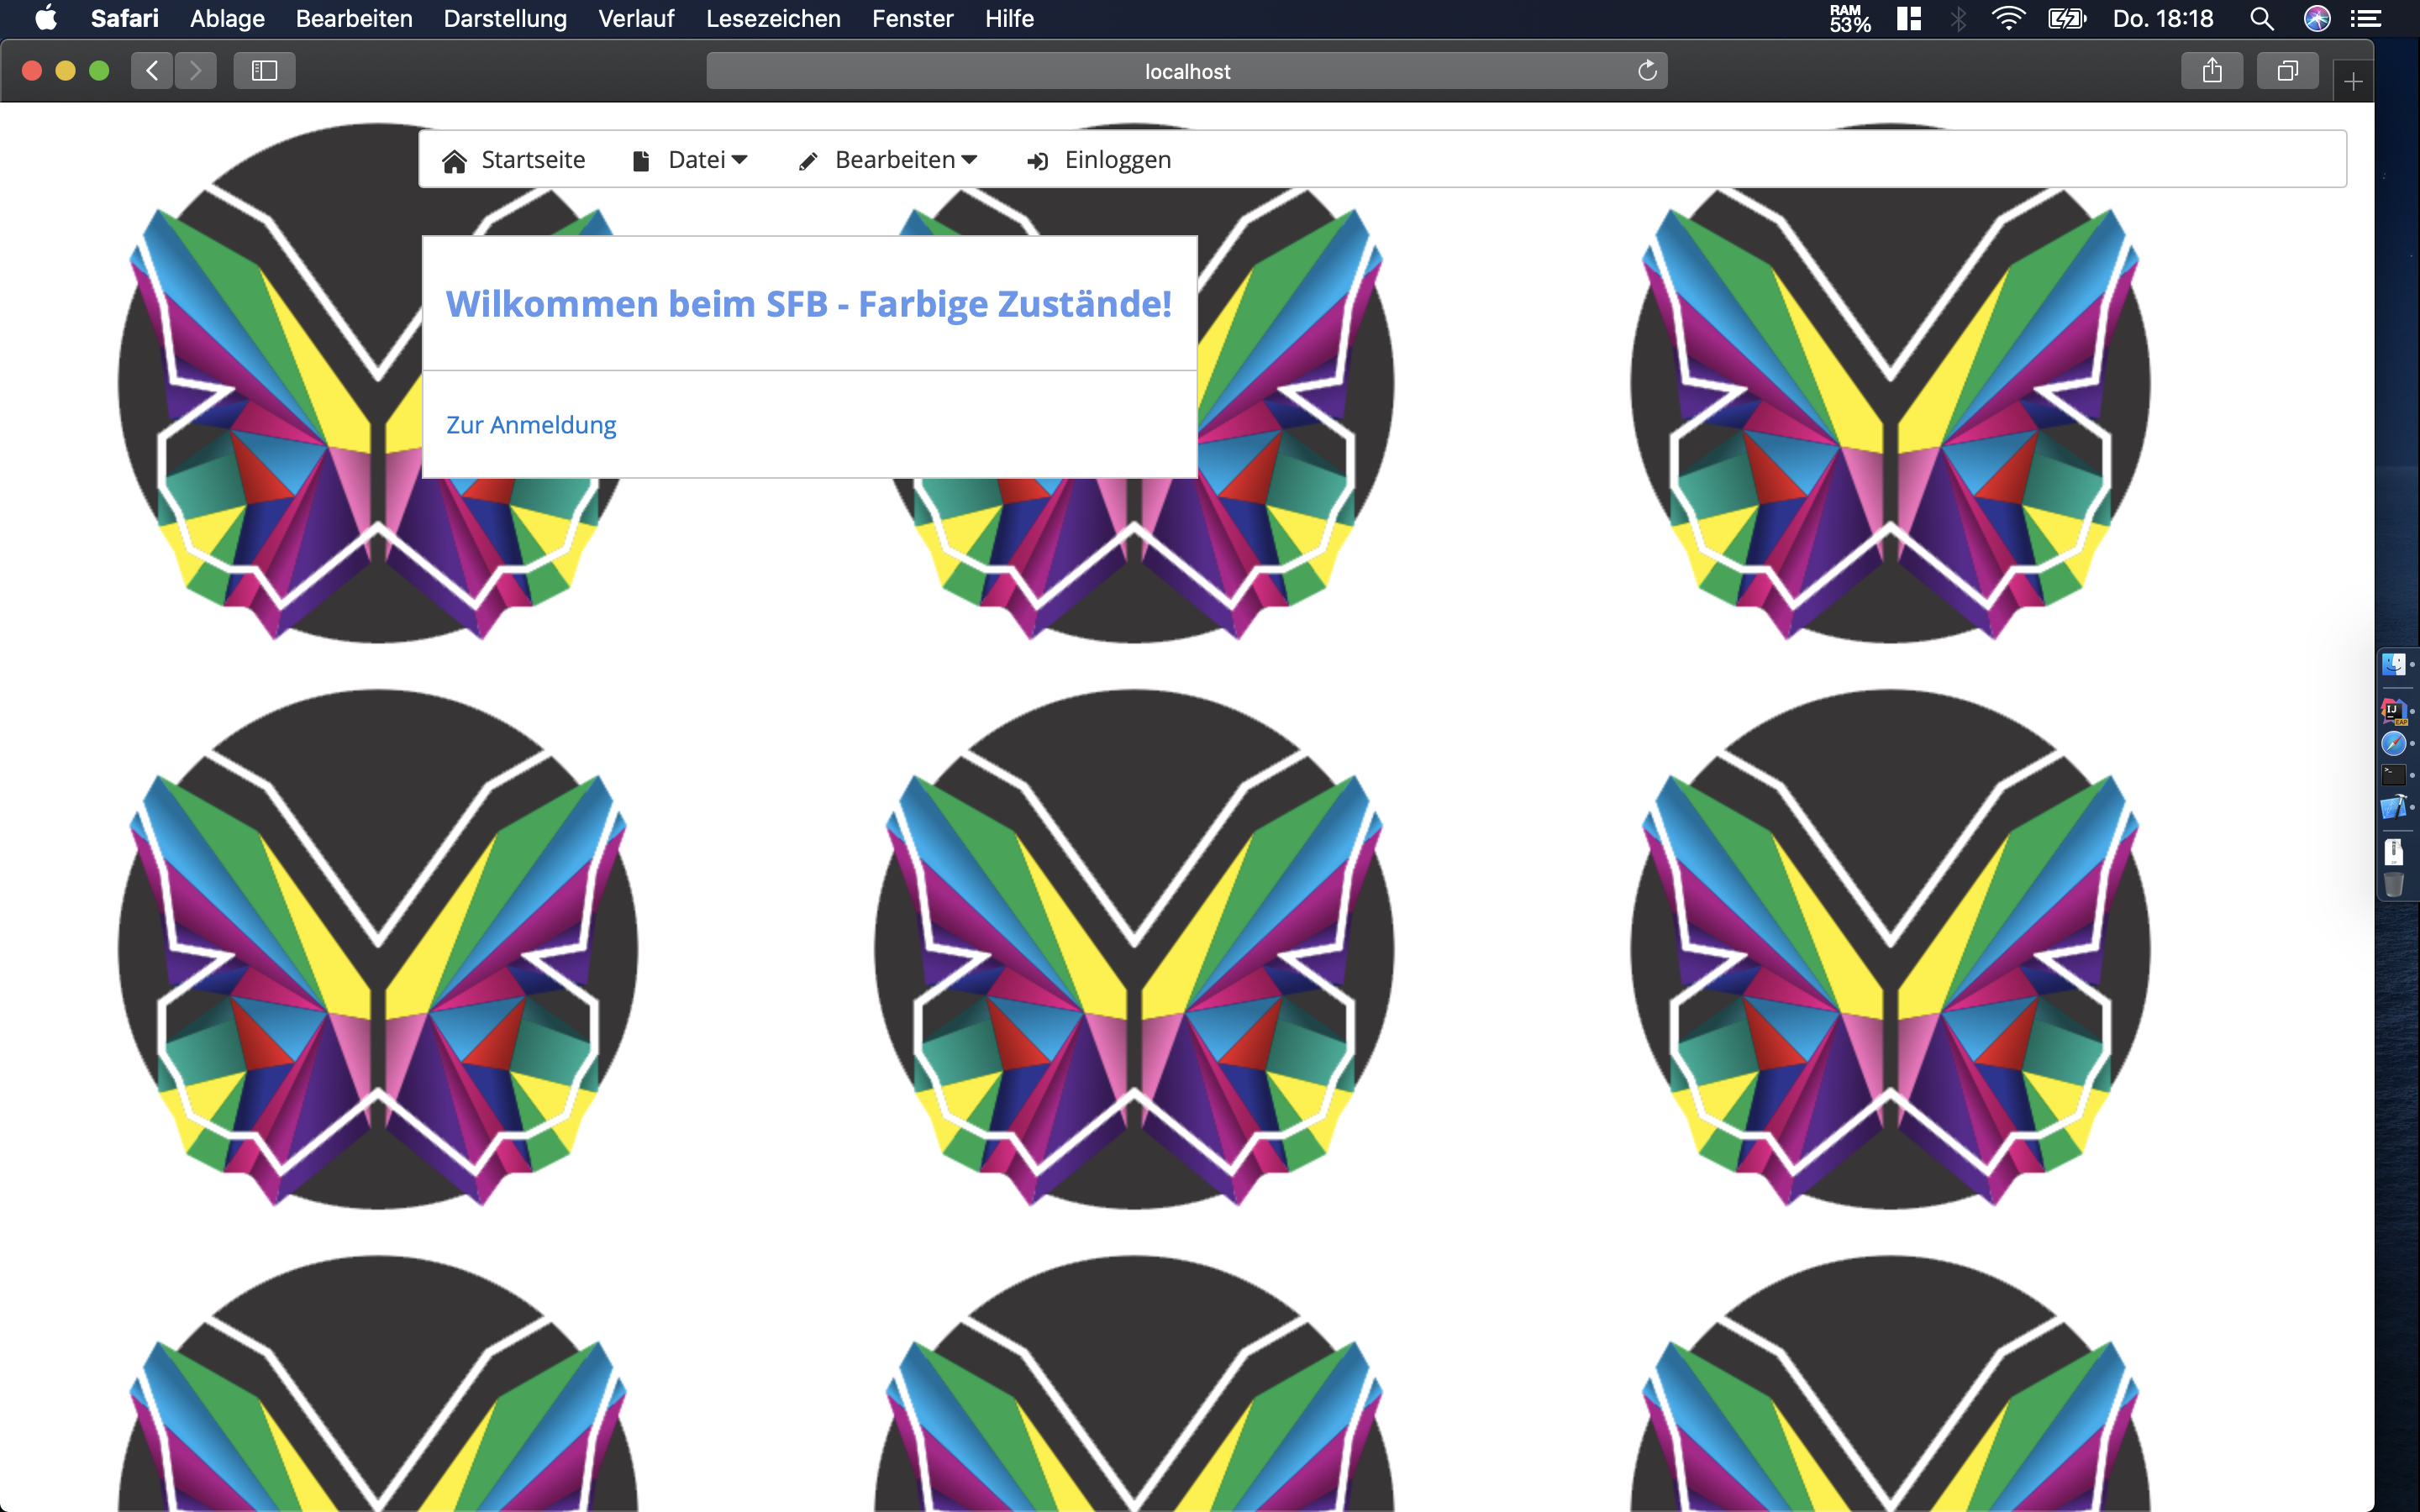
\includegraphics[width=1\textwidth]{Screenshots/311StartSite.png}
\textit{Abbildung 3.1.1.1: Startseite}
} \\

Hier kann man nun auf den Button \textit{Zur Anmeldung} drücken, um zur \hyperlink{sc3.1.1.2}{Loginseite} weitergeleitet zu werden. Ein valider Login ist der Benutzername \textit{admin} und das Passwort \textit{12345678}. \\

\hypertarget{sc3.1.1.2}{
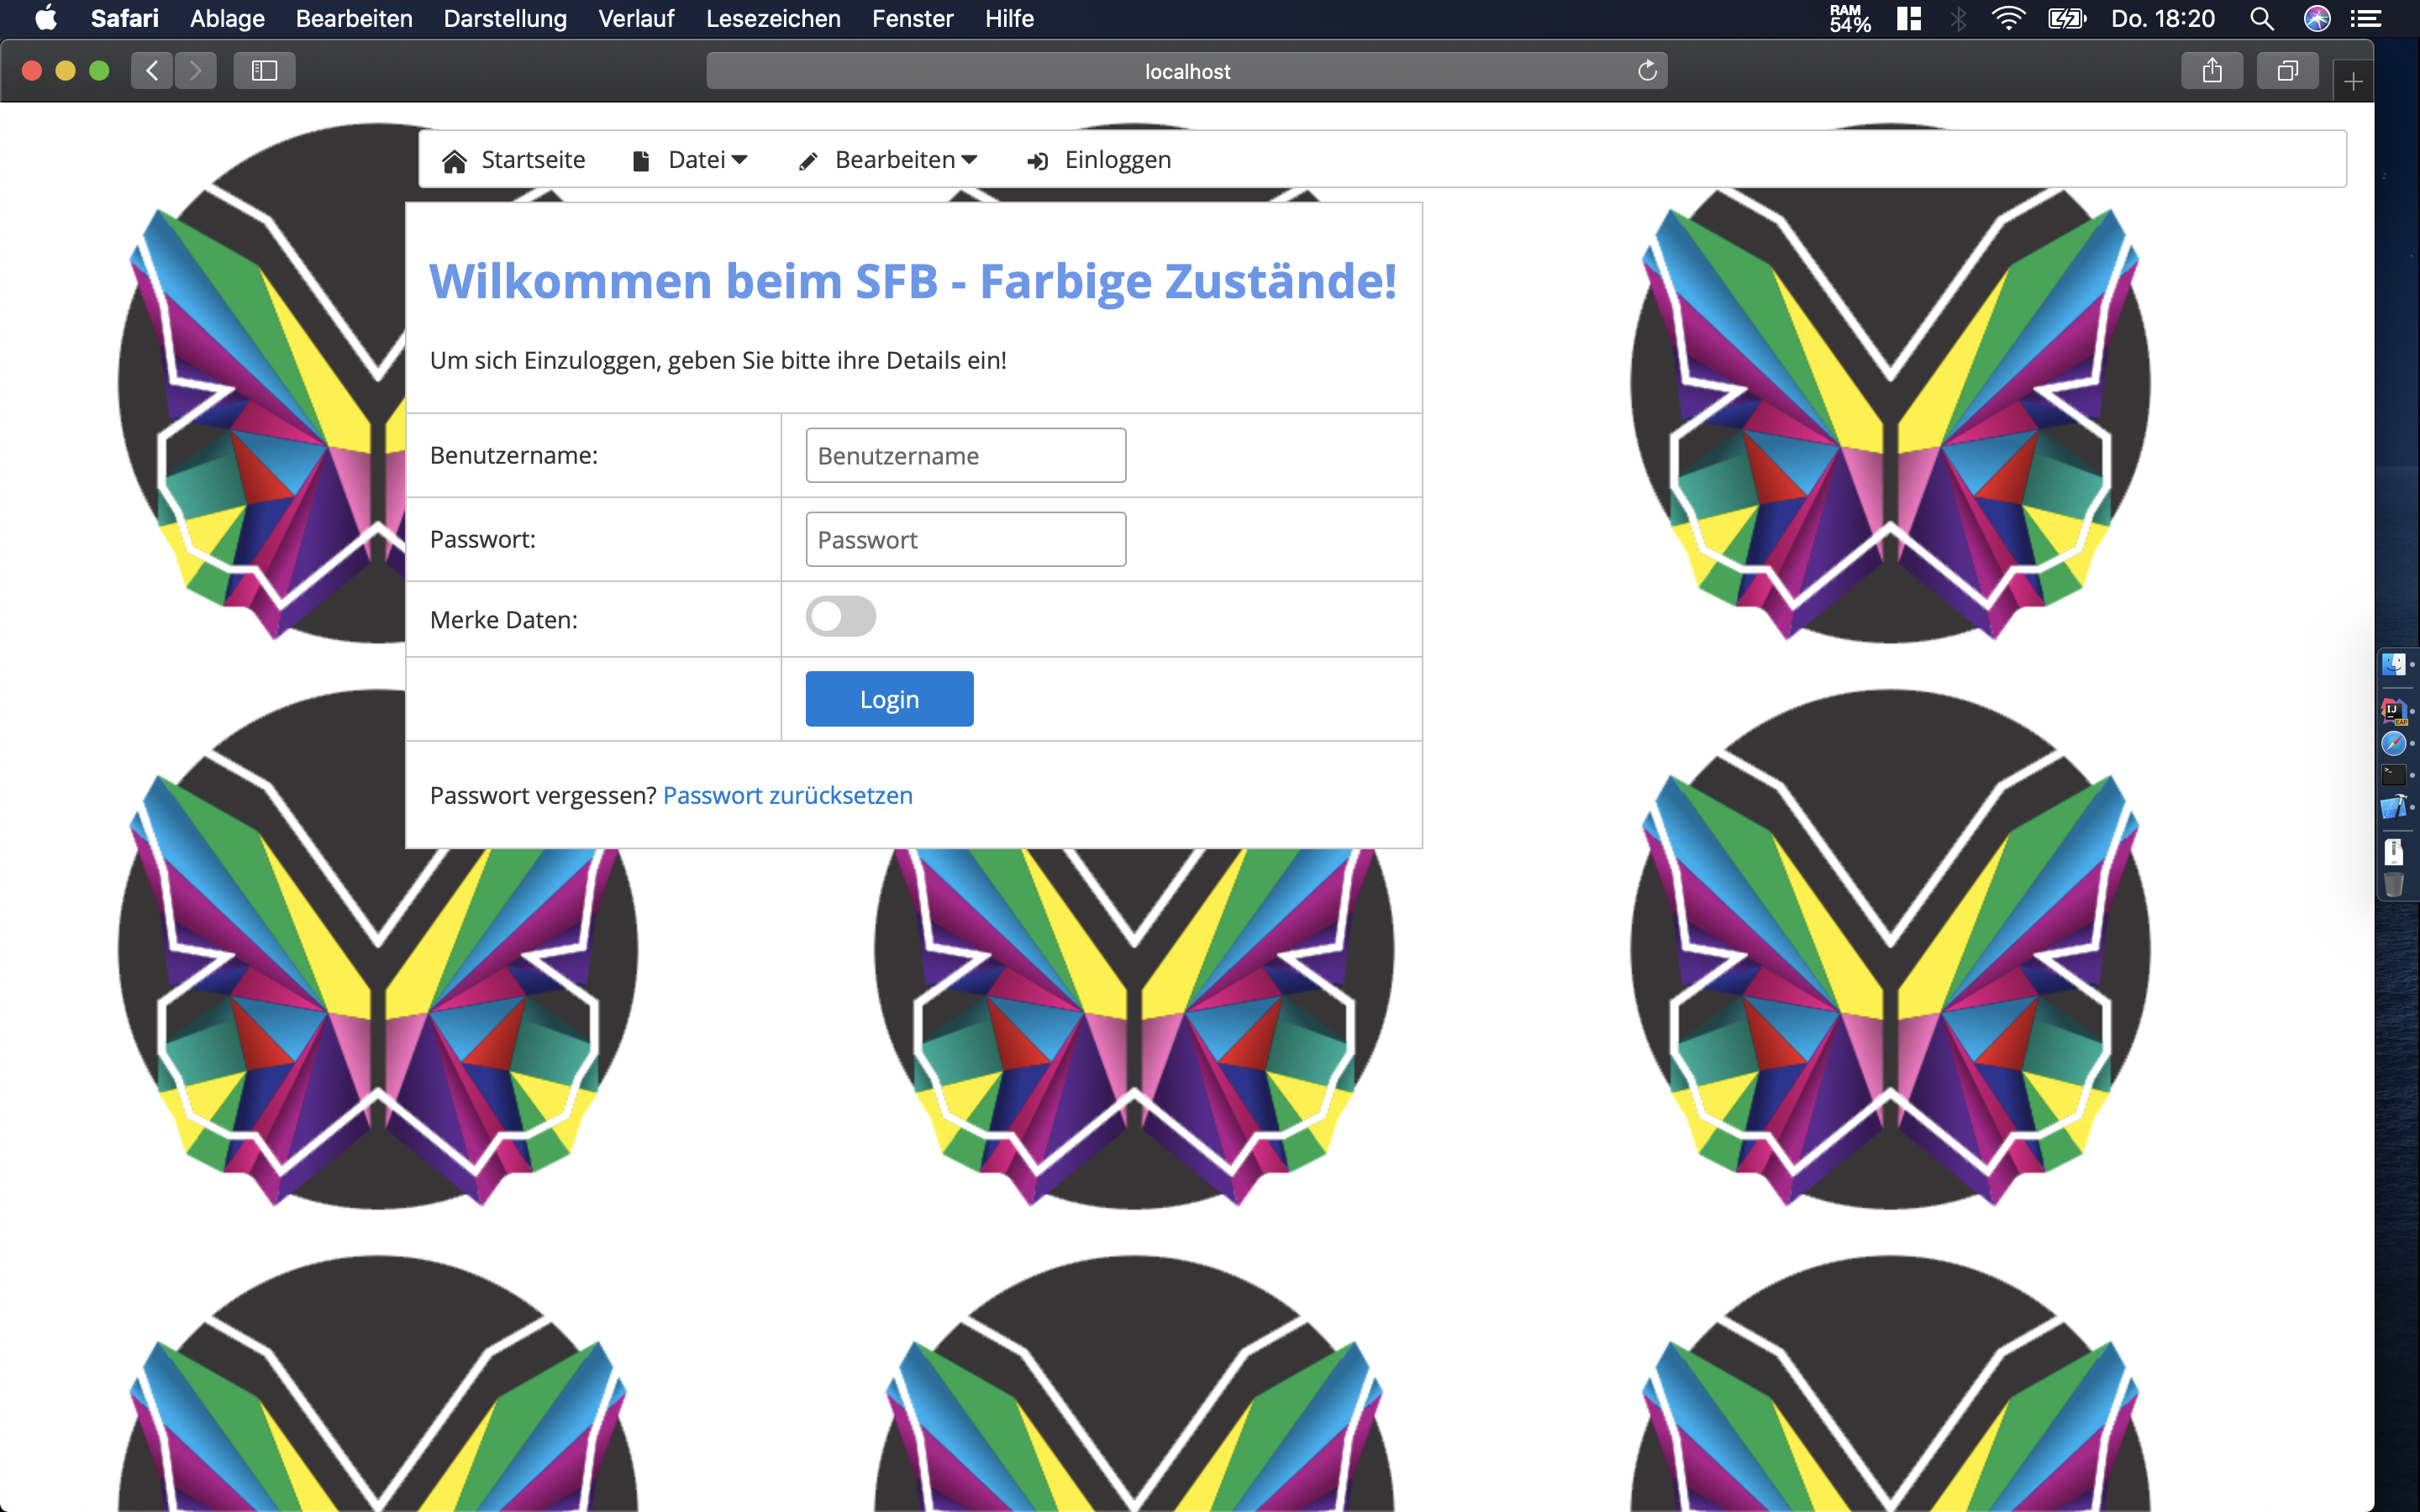
\includegraphics[width=1\textwidth]{Screenshots/311LoginSite.png}
\textit{Abbildung 3.1.1.2: Loginseite}
} \\

Jetzt haben wir uns als erstes mit einem falschen Passwort angemeldet, was eine Fehlermeldung wirft, wie man auf dem nächsten  \hyperlink{sc3.1.1.3}{Screenshot} in der oberen Ecke sieht.\\

\hypertarget{sc3.1.1.3}{
\includegraphics[width=1\textwidth]{Screenshots/311wrongPassword.png}
\textit{Abbildung 3.1.1.3: Falsches Passwort für Admin eingegeben}
} \\

Anschließend wurde versucht, sich mit den validen Logindaten des Admins einzuloggen und man kommt auf die \hyperlink{sc3.1.1.4}{Startseite des Admins}. \\

\hypertarget{sc3.1.1.4}{
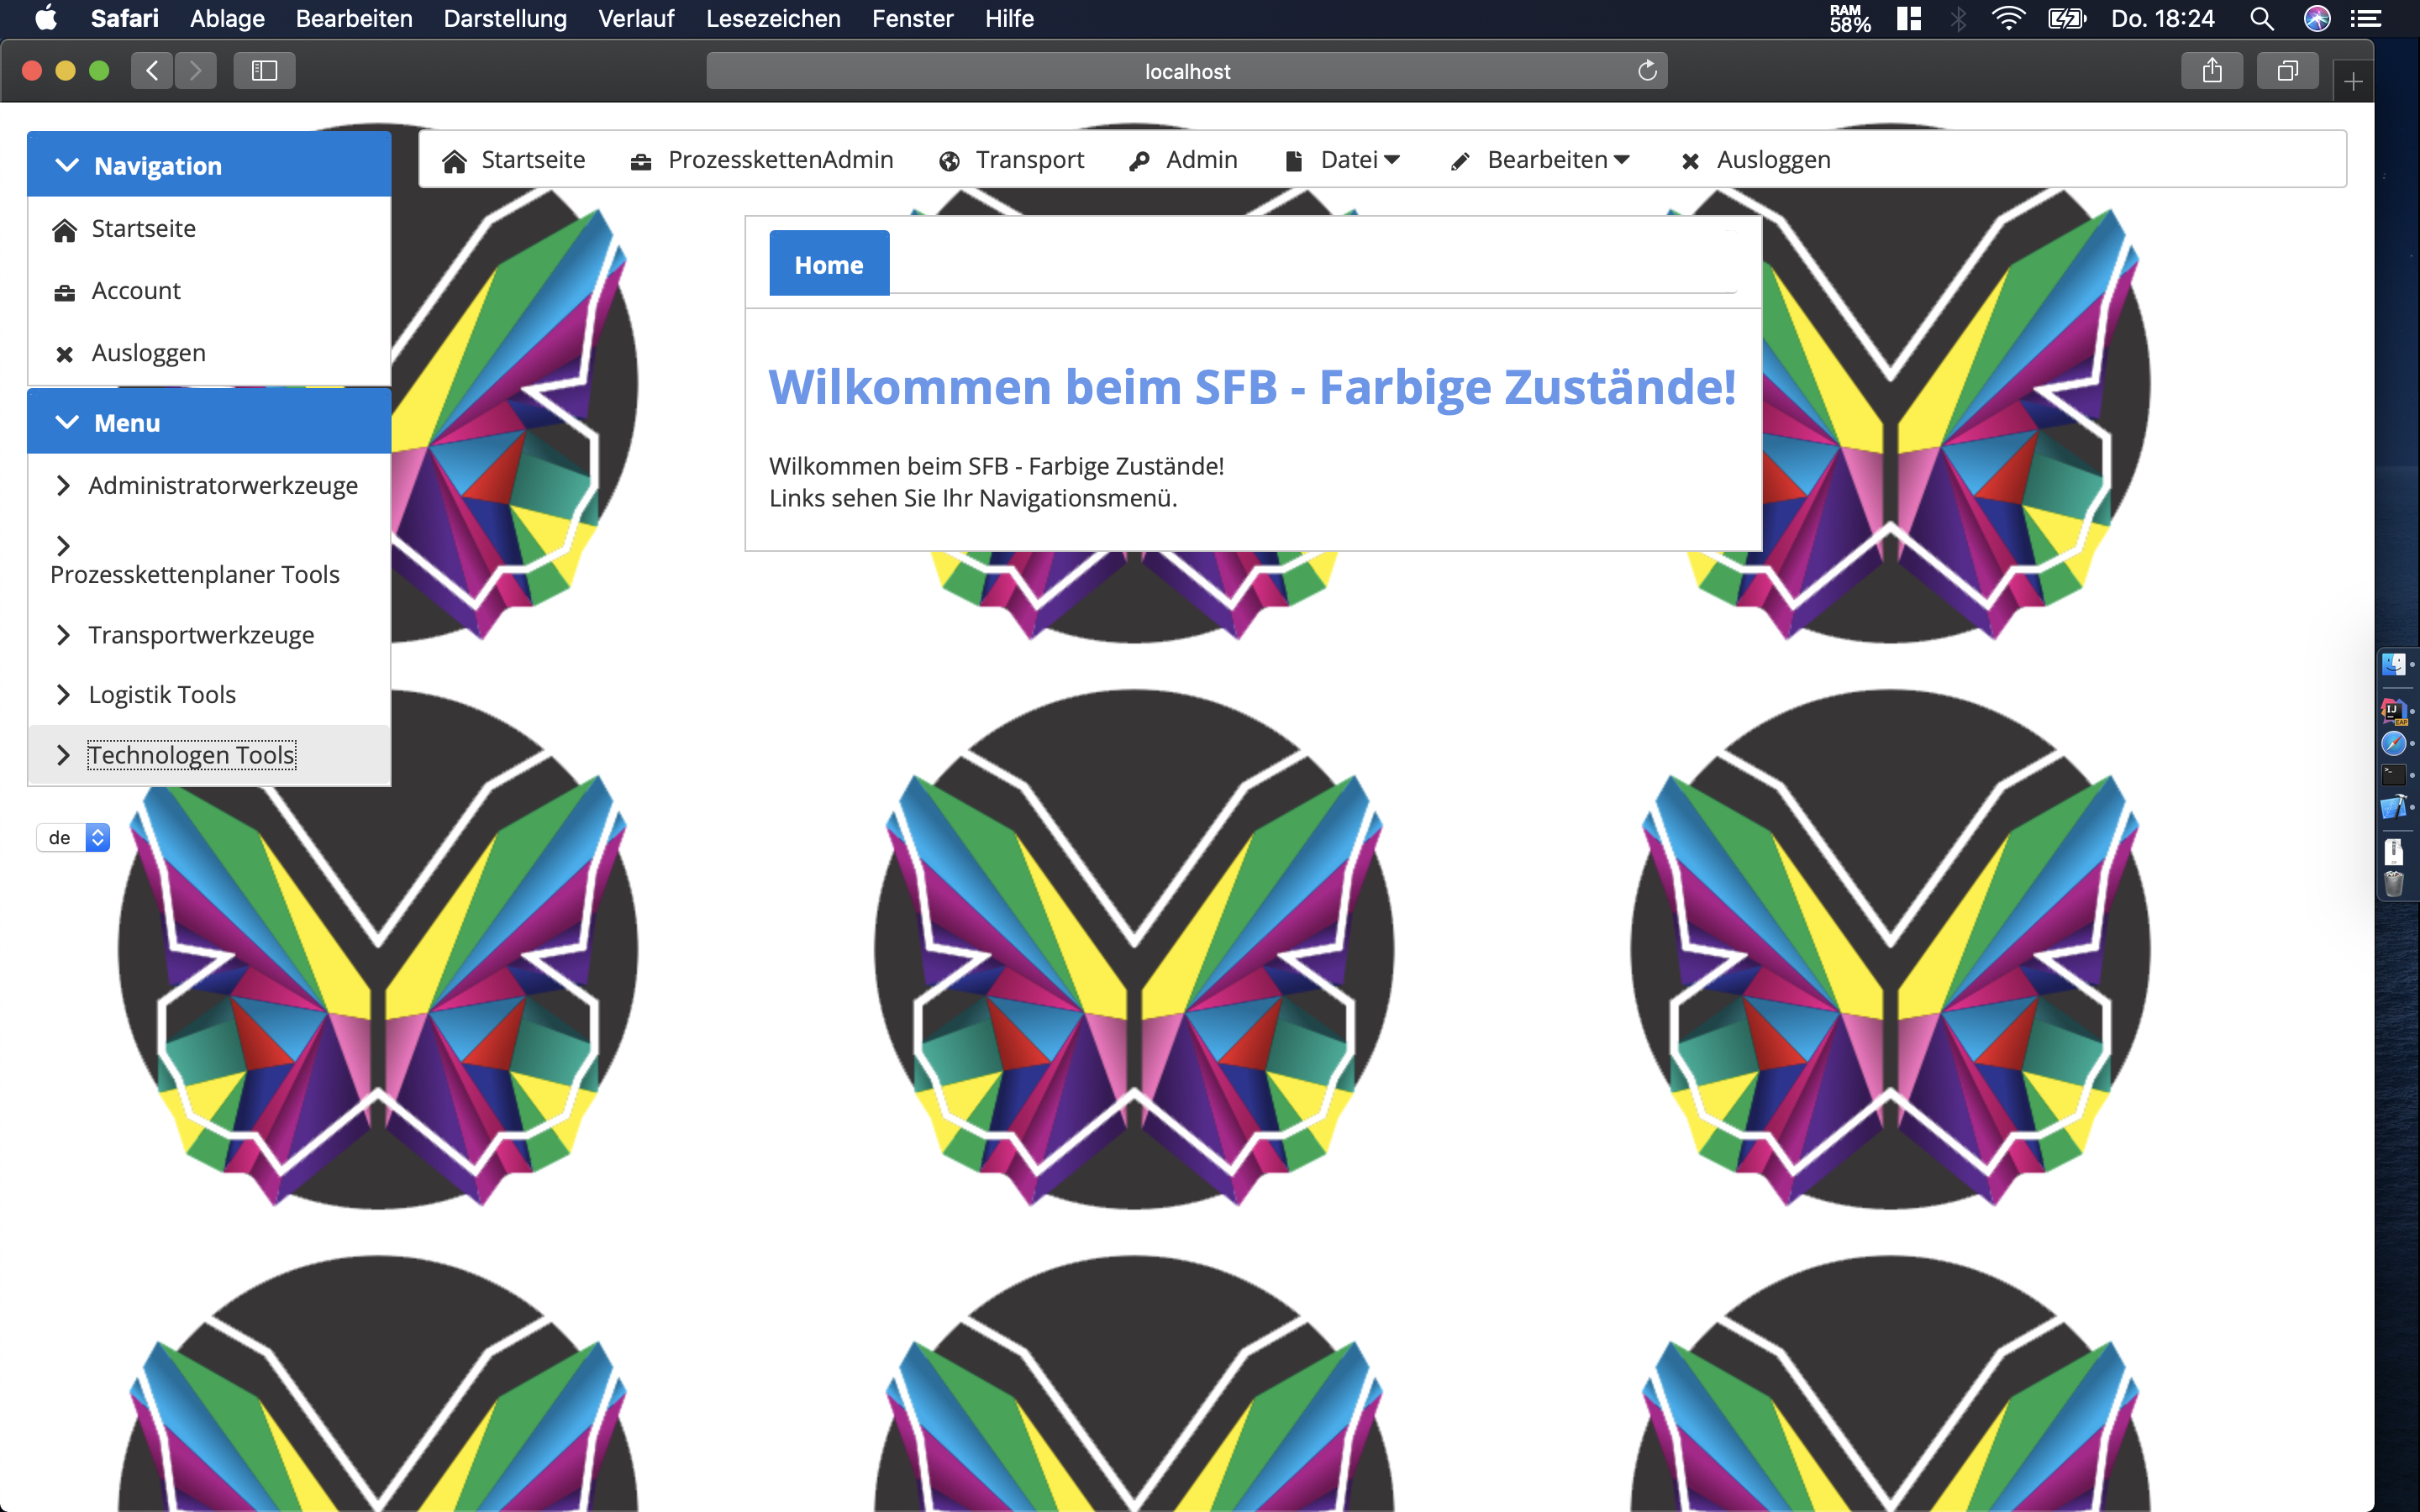
\includegraphics[width=1\textwidth]{Screenshots/311AdminView.png}
\textit{Abbildung 3.1.1.4: Richtiges Passwort für Admin eingegeben}
} \\

Jetzt wurde sich noch versucht, mit den validen Logindaten für den Technologen einzuloggen. Man wird auf die \hyperlink{sc3.1.1.5}{Startseite des Technologen} weitergeleitet. \\

\hypertarget{sc3.1.1.5}{
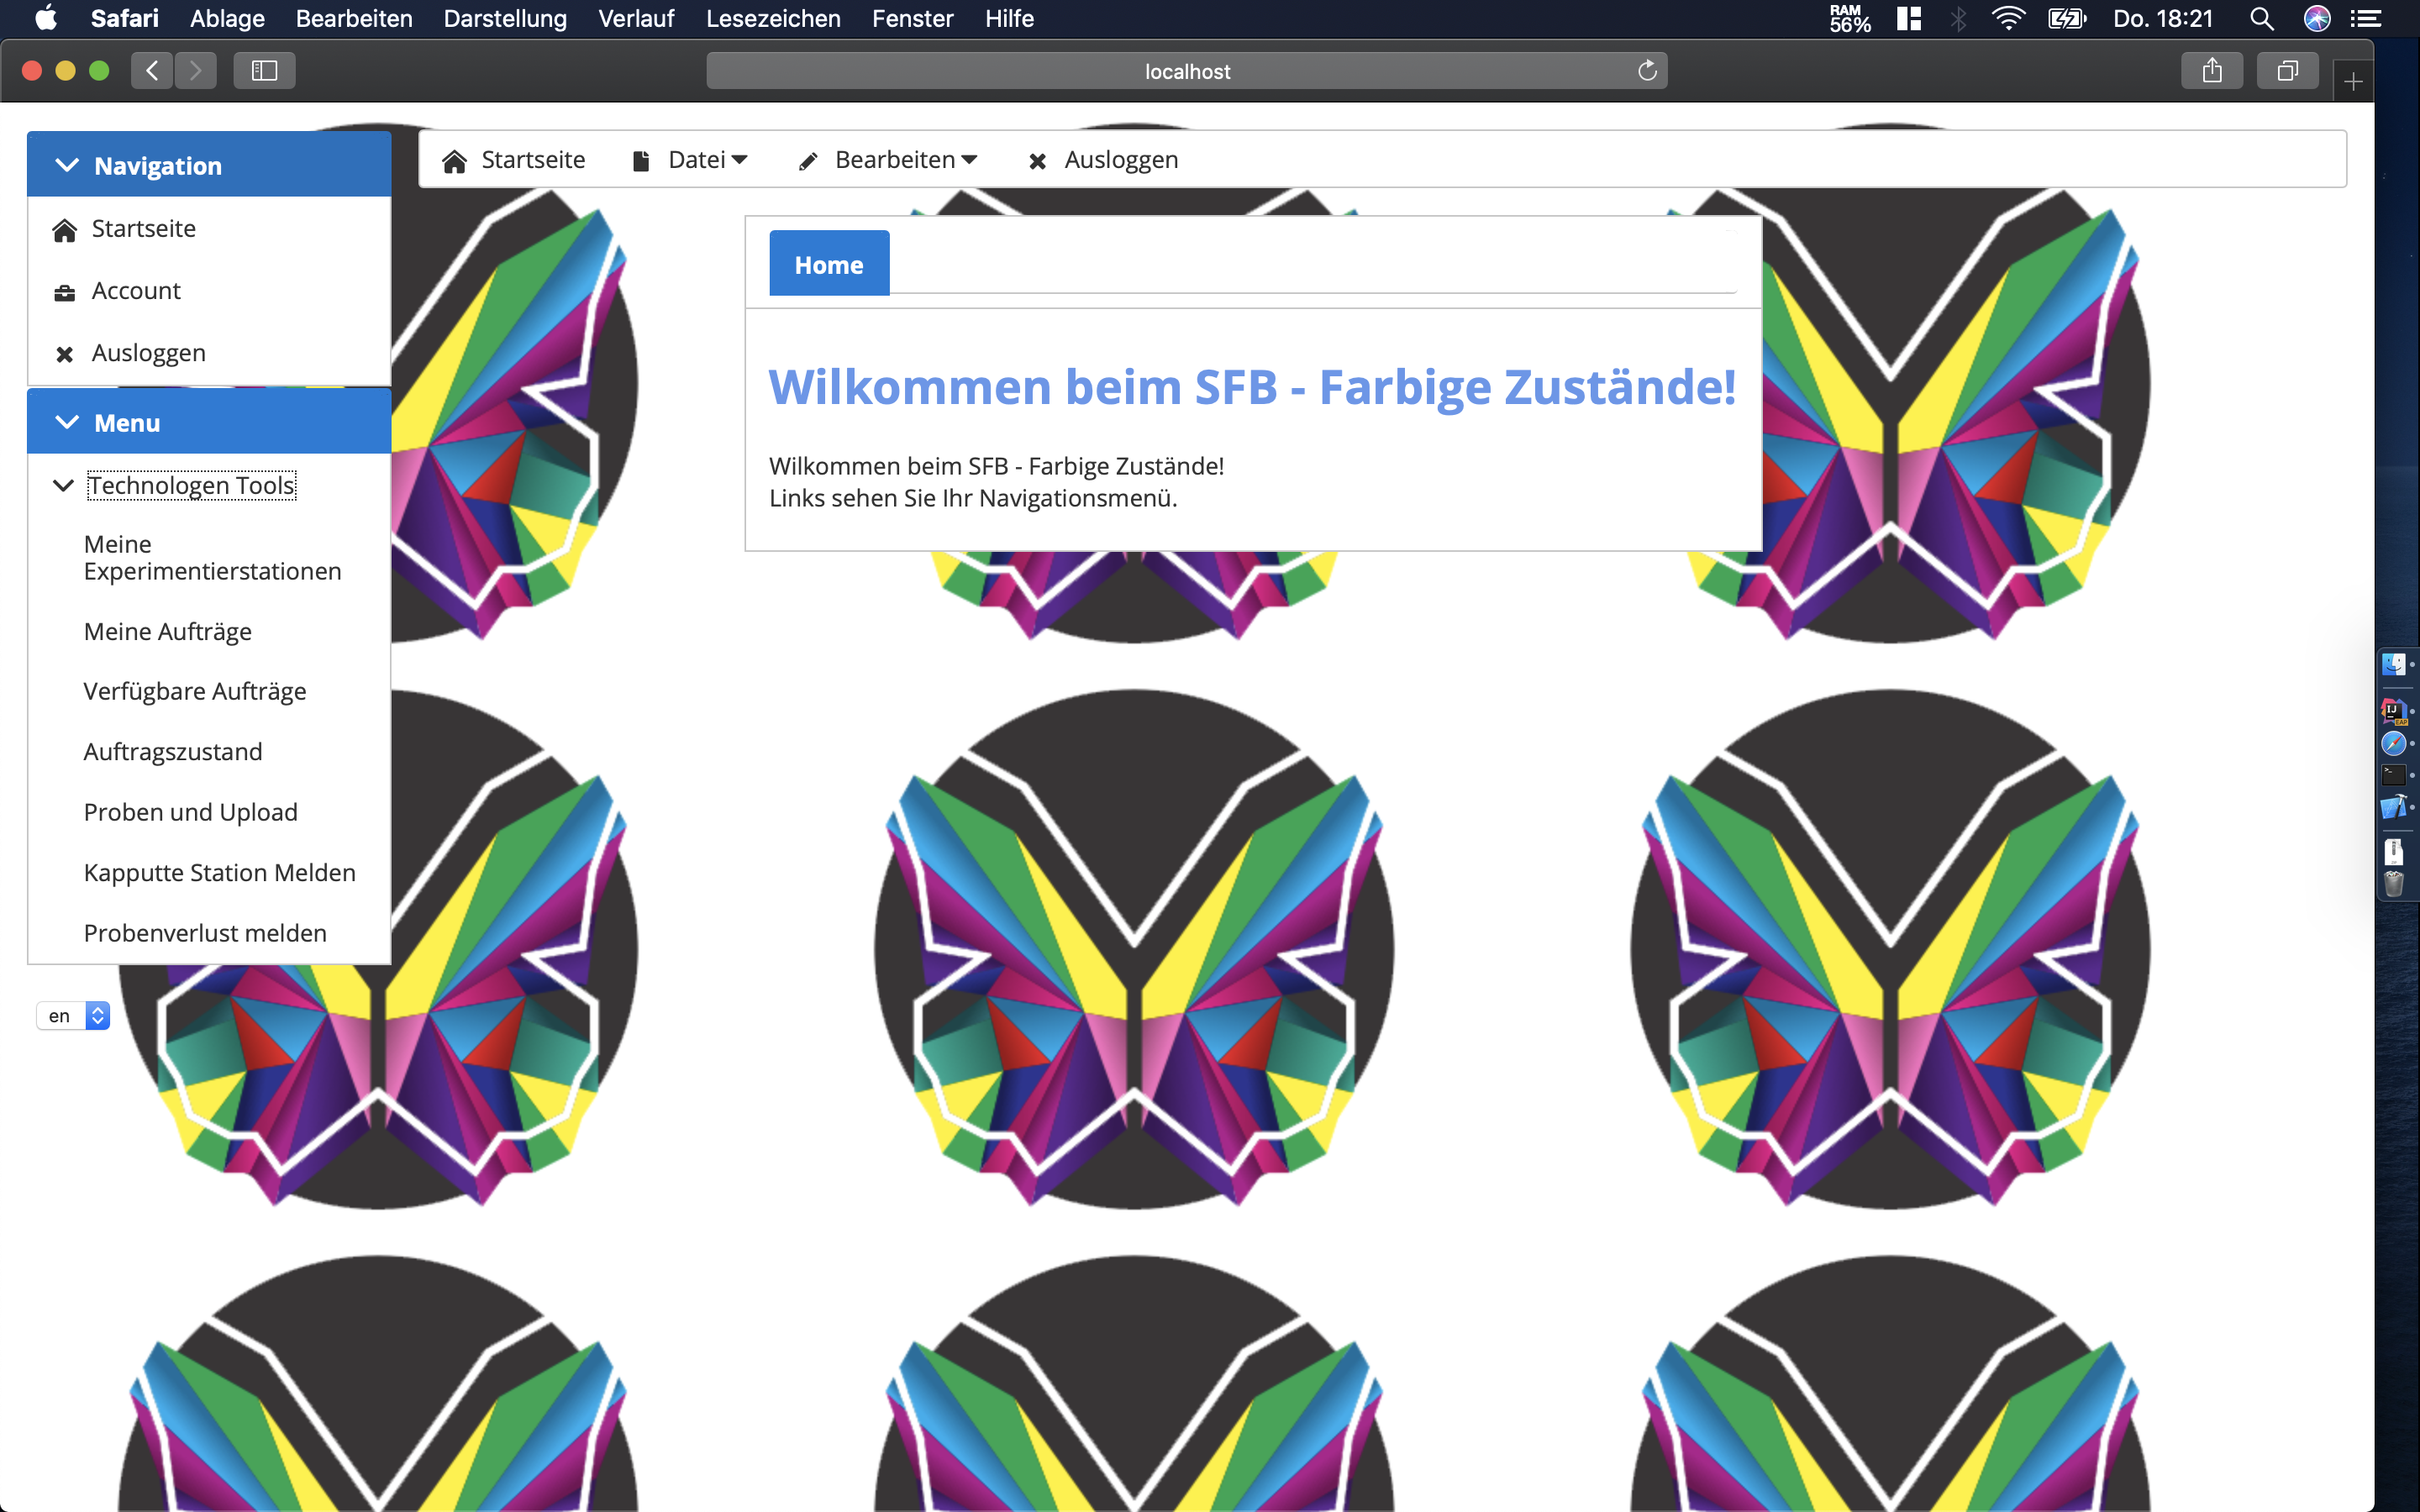
\includegraphics[width=1\textwidth]{Screenshots/311TechnologeView.png}
\textit{Abbildung 3.1.1.5: Richtiges Passwort für Technologen eingegeben}
} \\

Wie man in den Beispielen sehen kann, kann man sich mit unterschiedlichen Benutzern einloggen, welche unterschiedliche den Rollen entsprechende Features haben. Man muss das richtige Passwort für den Benutzernamen eingeben, um sich einloggen zu können. Die Tests verliefen erfolgreich. \\ 

\hypertarget{sc3.1.1.6}{
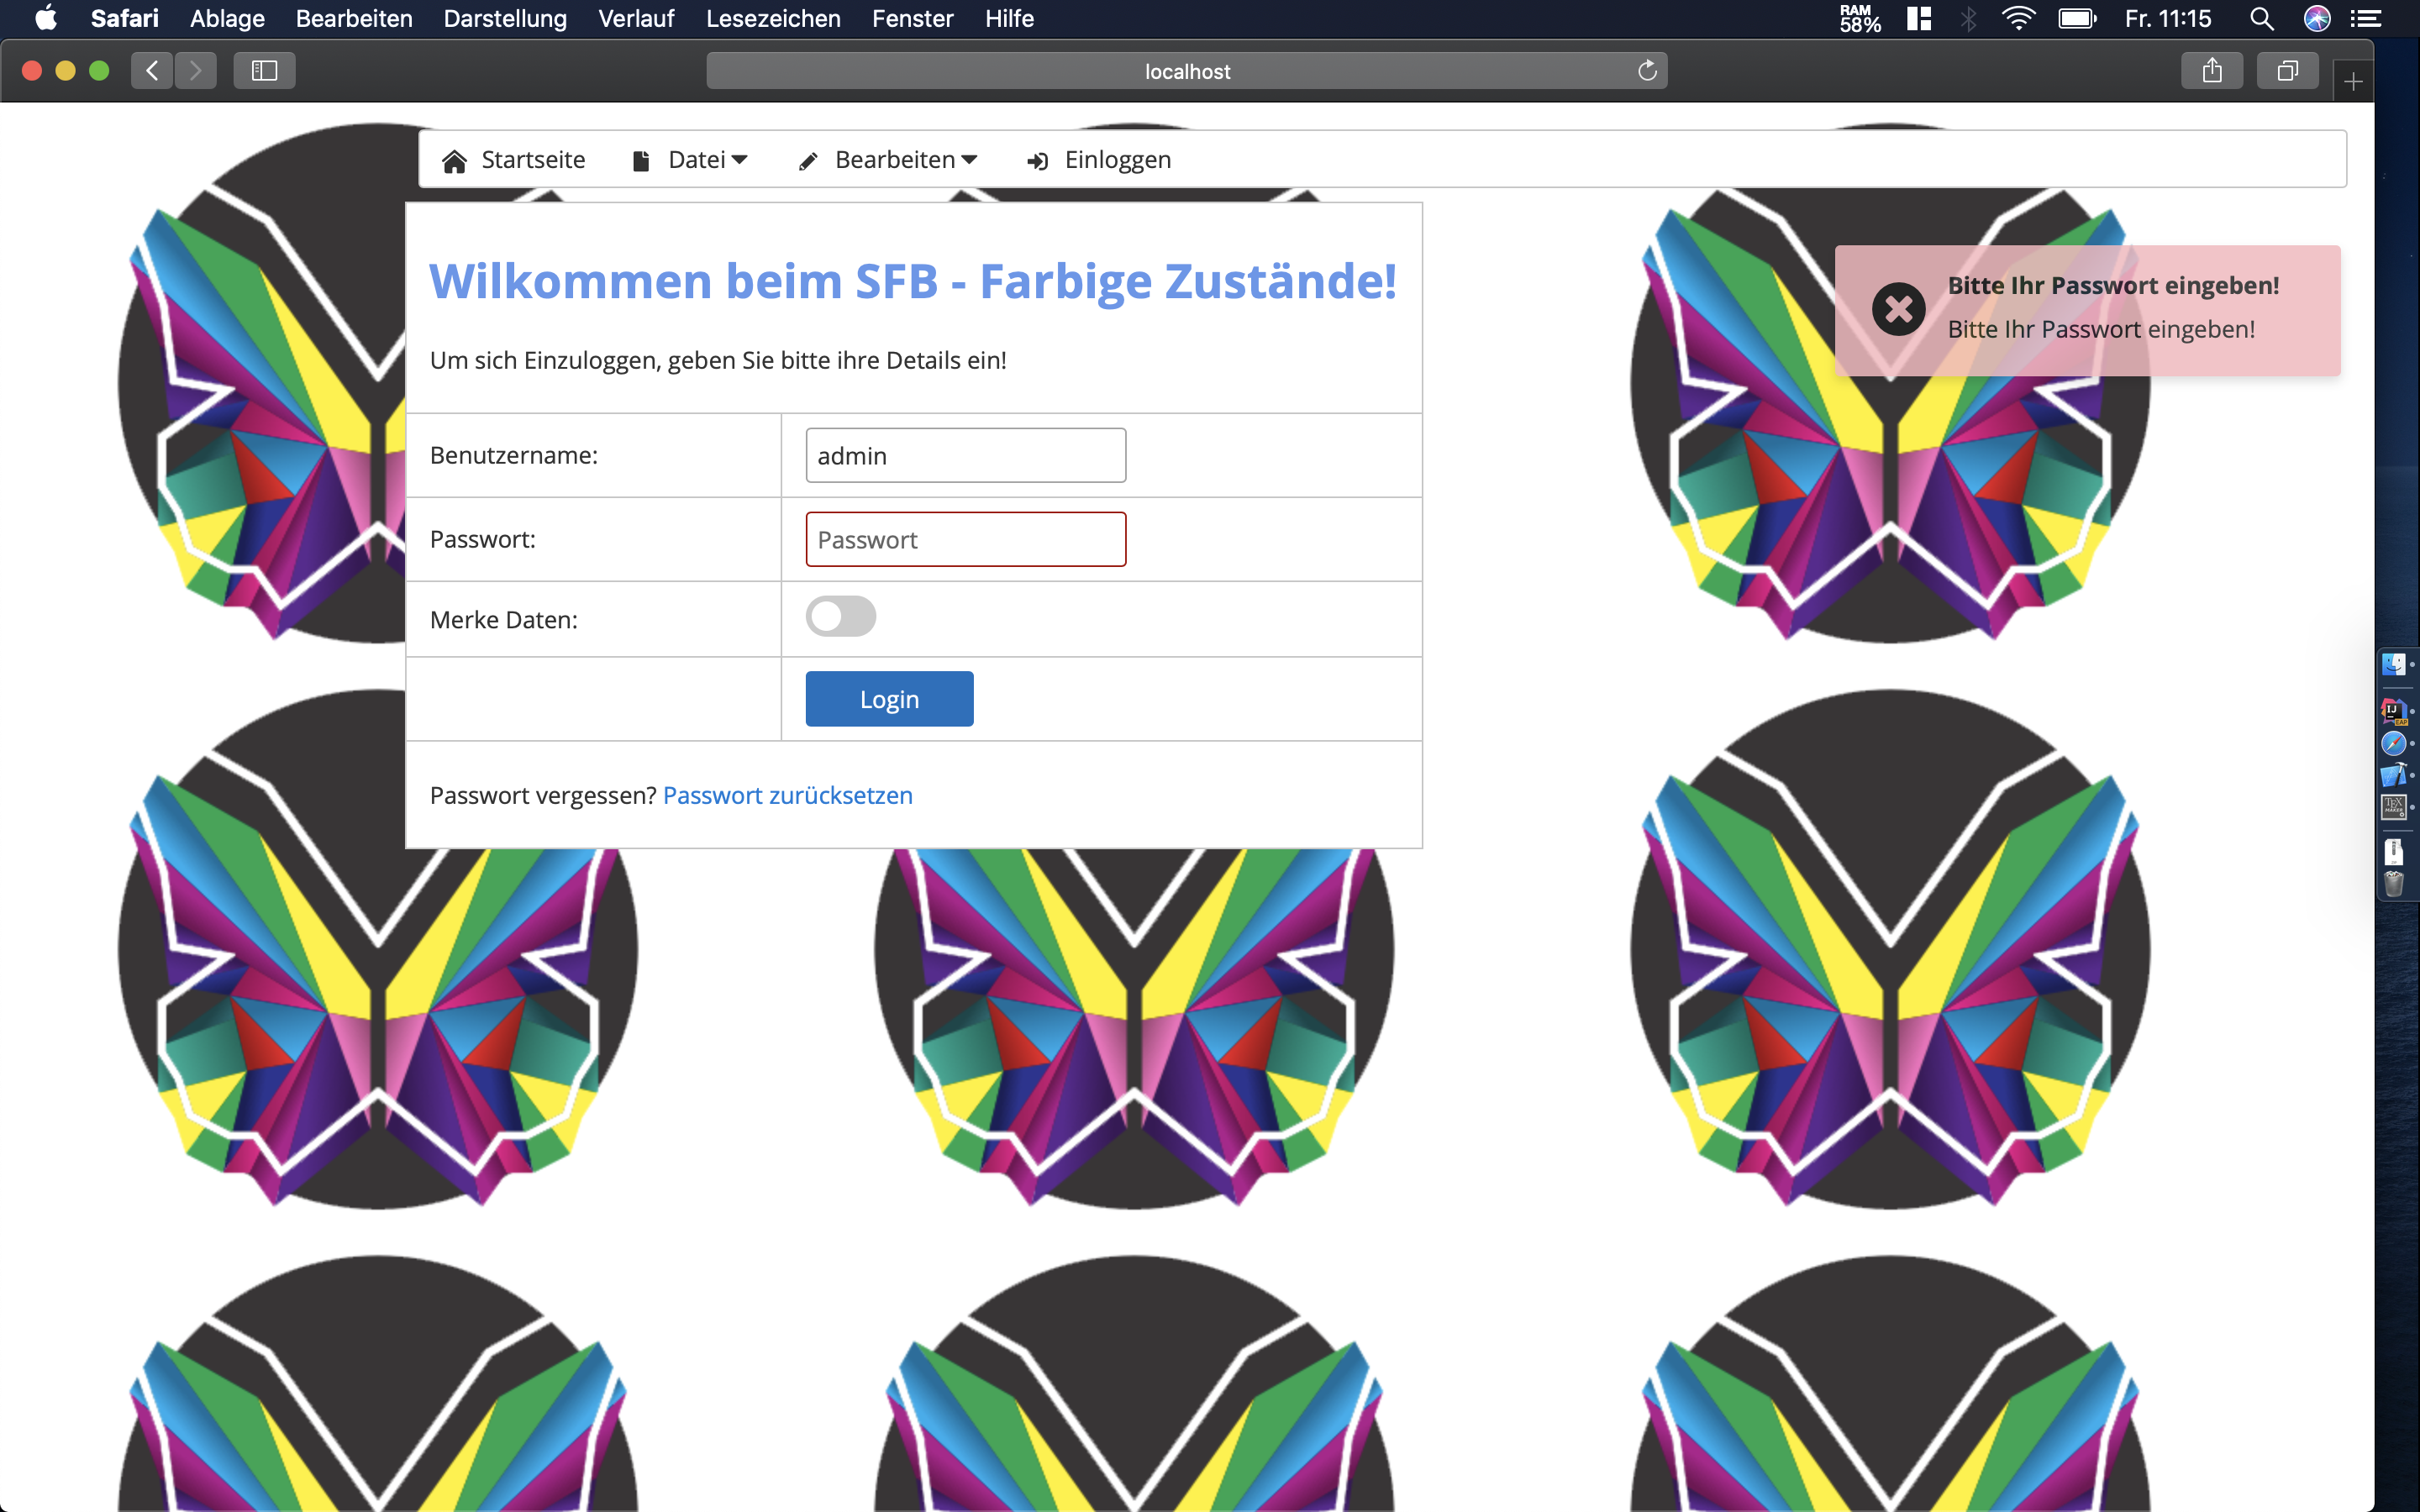
\includegraphics[width=1\textwidth]{Screenshots/311BittePasswordEingeben.png}\\ \textit{Abbildung 3.1.1.6: Benutzer ohne password}
} \\

\hypertarget{sc3.1.1.7}{
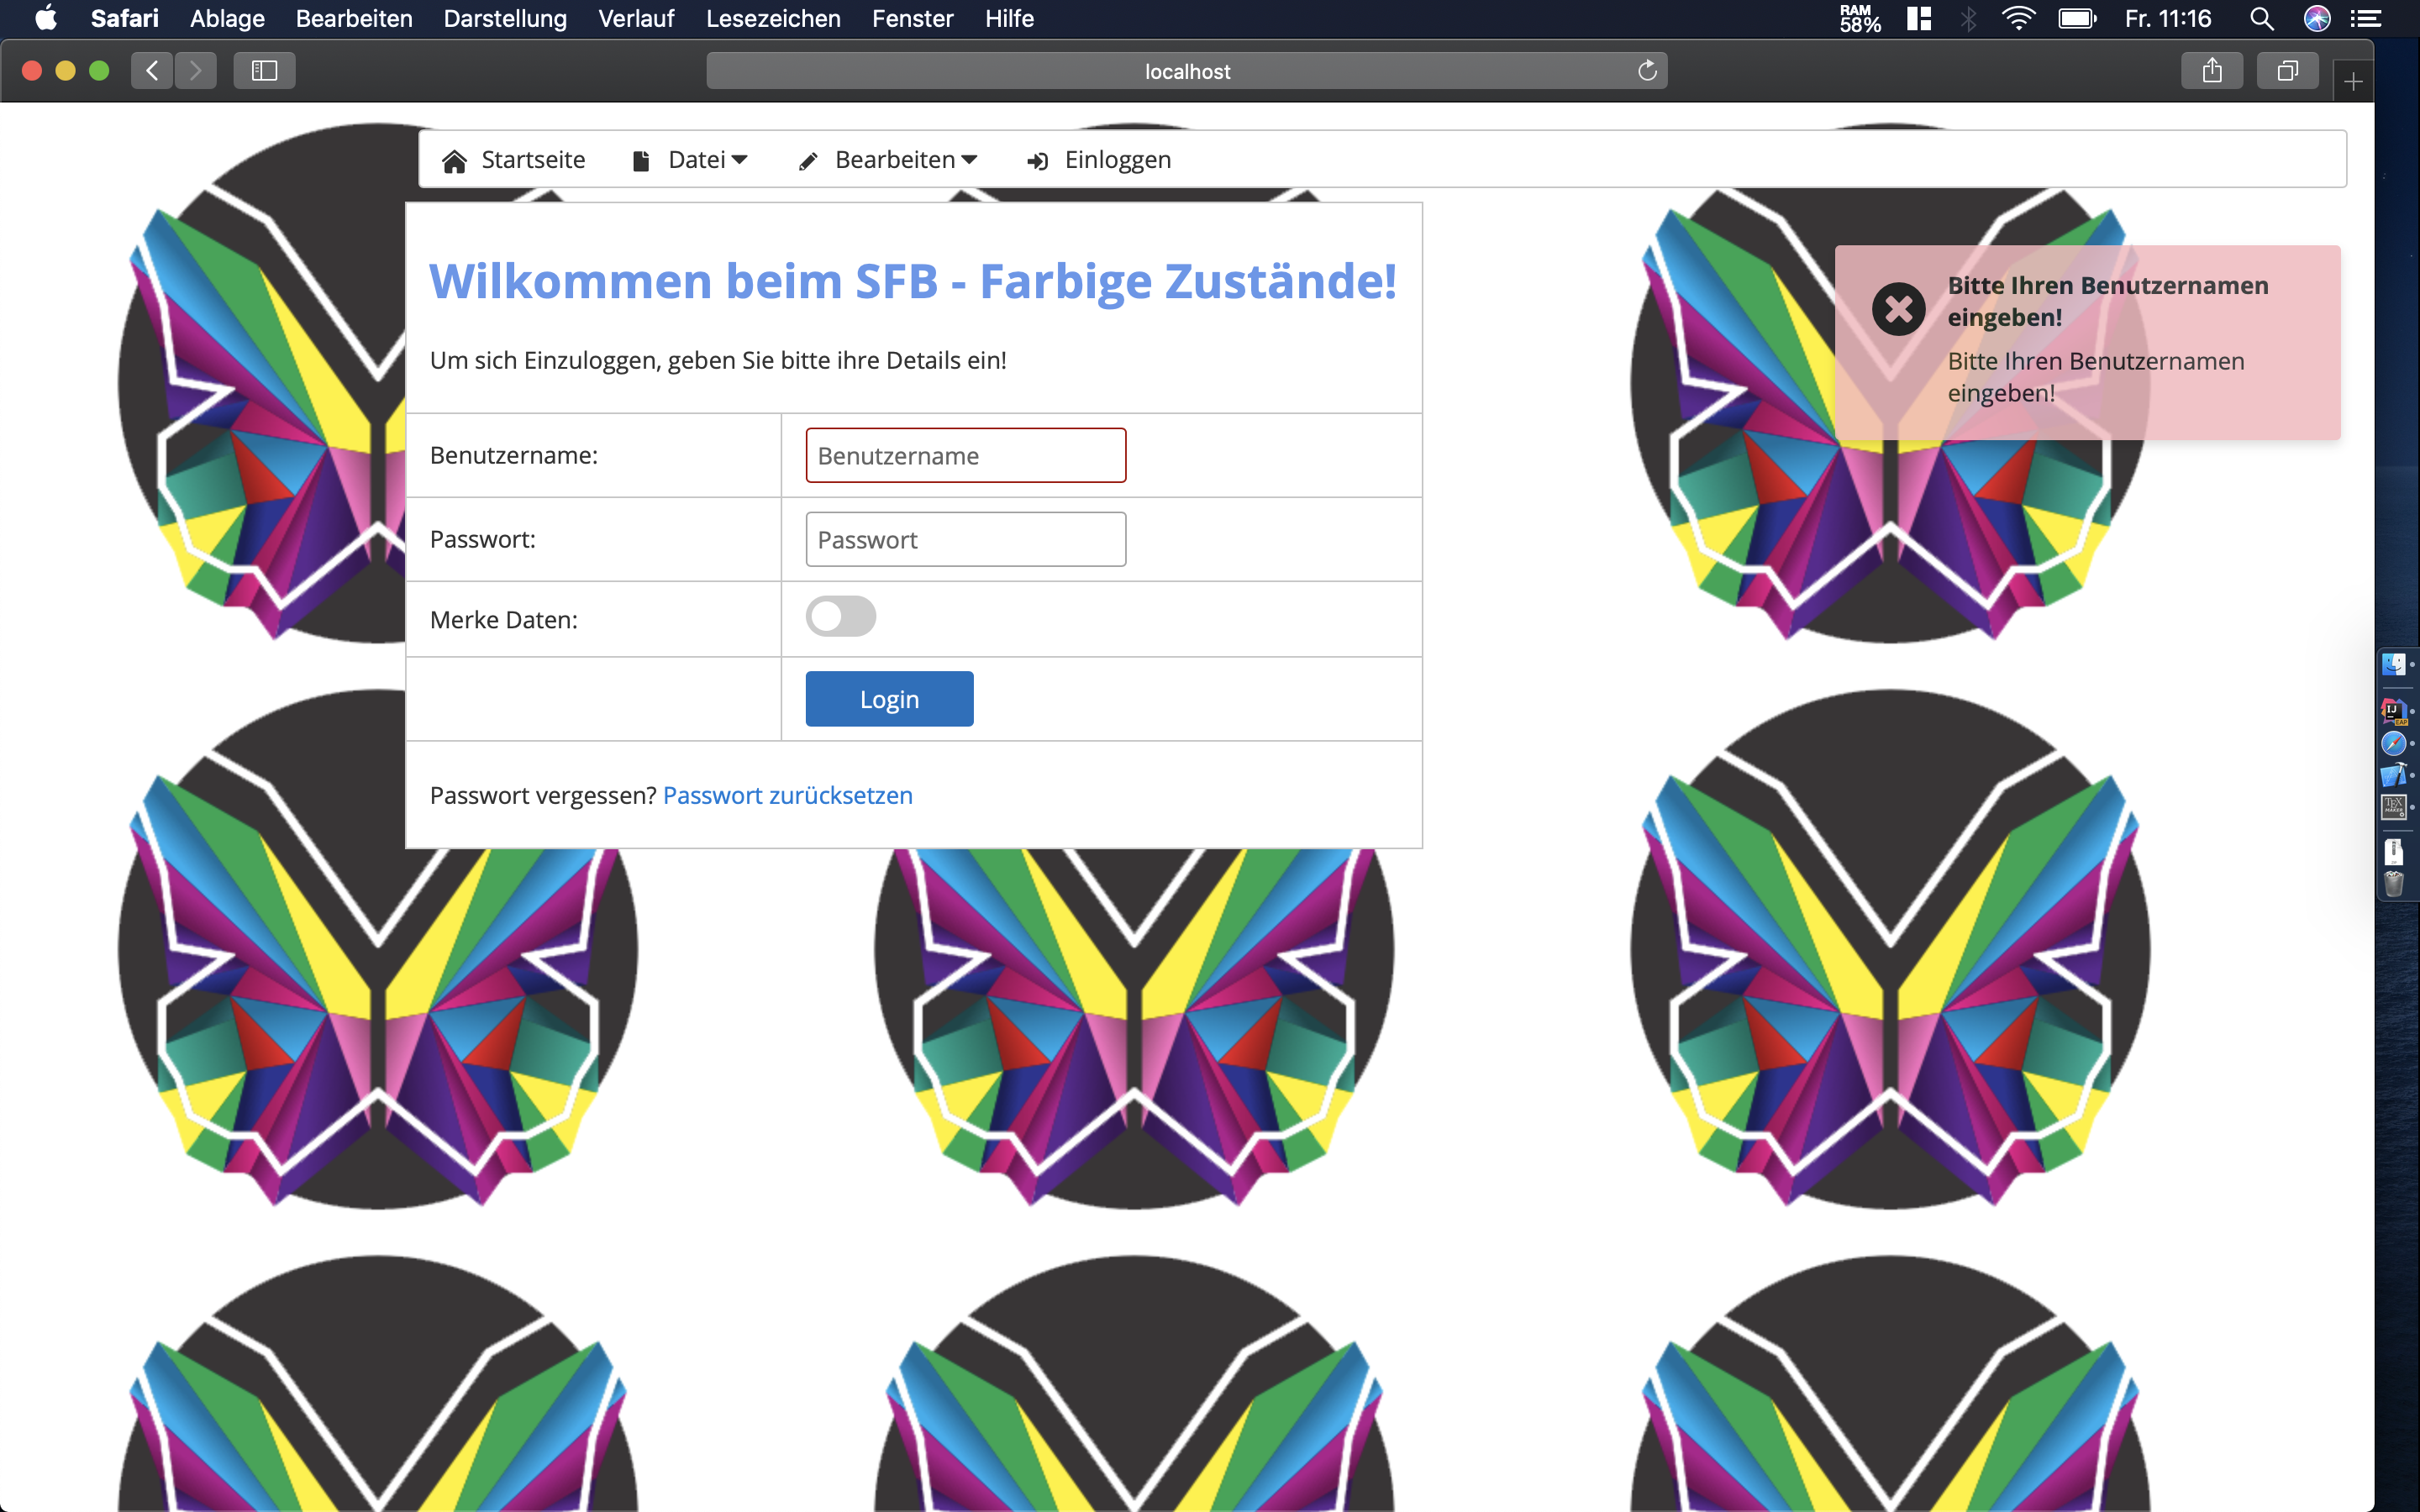
\includegraphics[width=1\textwidth]{Screenshots/311PasswordohneBenutzer.png}
\textit{Abbildung 3.1.1.7: password ohne Benutzer}
} \\


Für die Erstellung und Kontrolle der Benutzer verfügt der Administrator über eine Tabelle und ein Formular.

Nun haben wir noch getestet, was passiert, wenn kein Benutzername eingegeben wird. Wie man sieht, wird eine  \hyperlink{sc3.1.1.8}{Fehlermeldung} ausgegeben. \\

\hypertarget{sc3.1.1.8}{
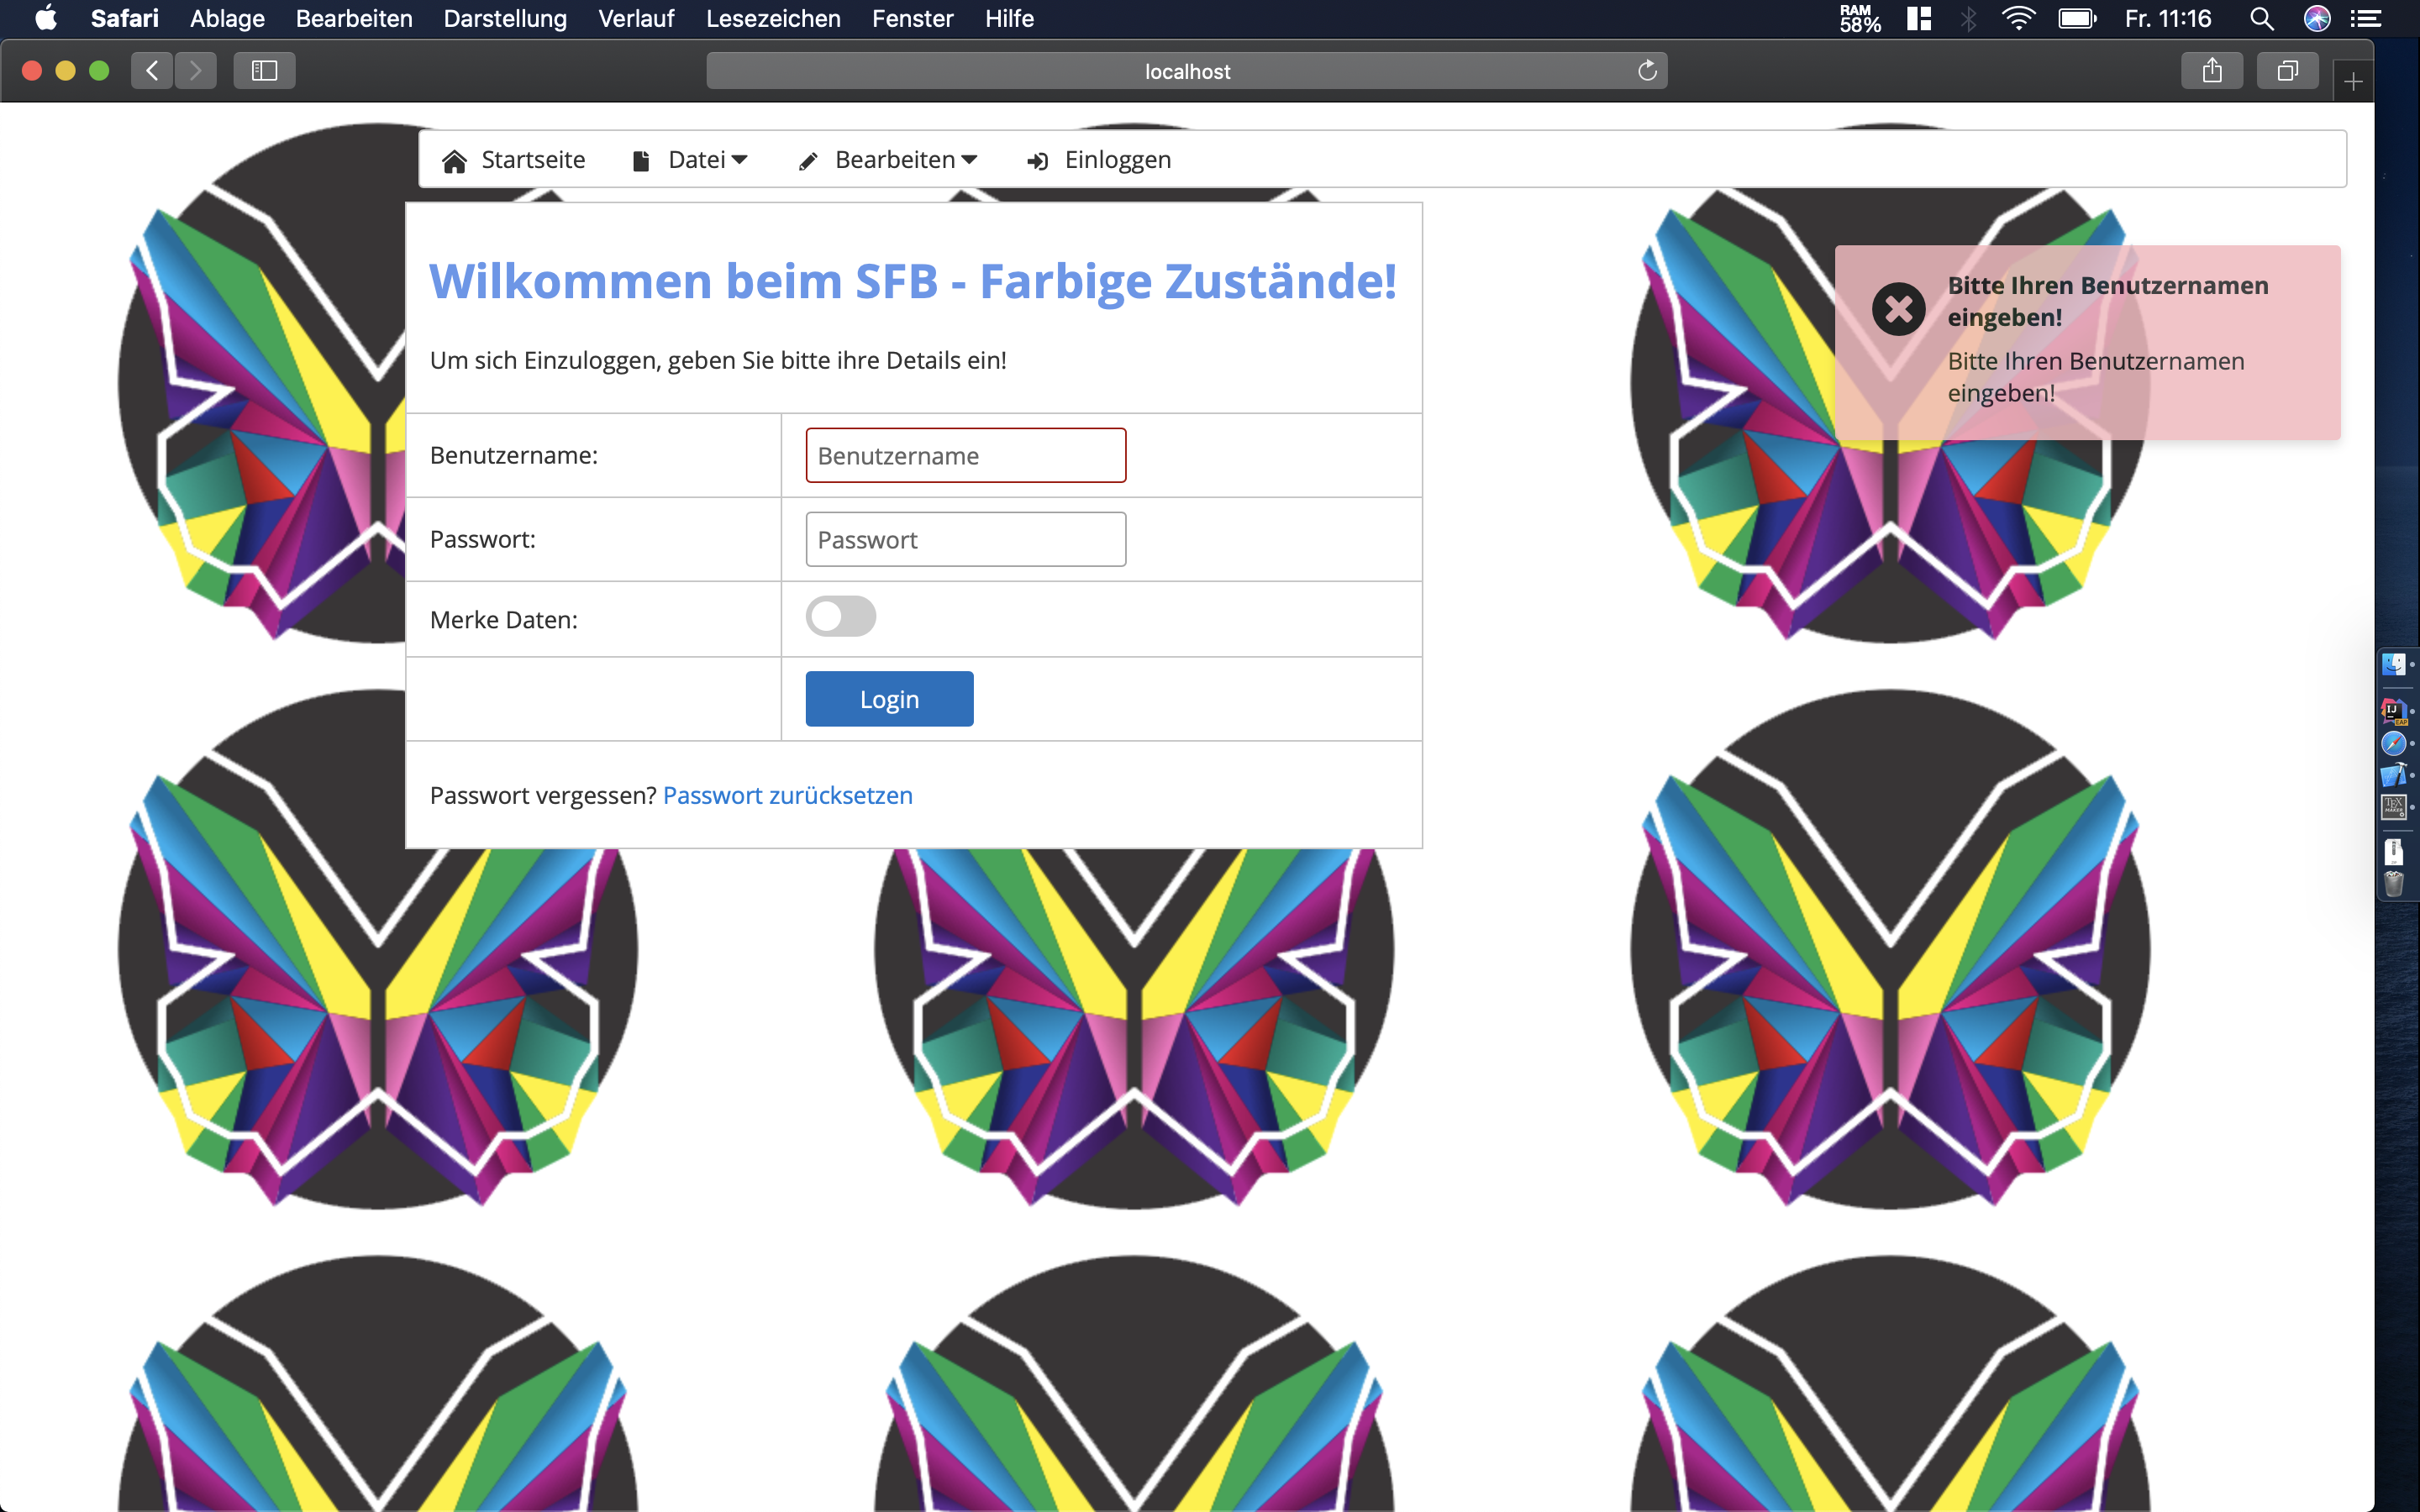
\includegraphics[width=1\textwidth]{Screenshots/311PasswordohneBenutzer.png}
\textit{Abbildung 3.1.1.8: Fehlermeldung: Bitte Ihren Benutzernamen eingeben!}
} \\

Zuletzt wurde getestet, was passiert, wenn kein Passwort eingegeben wurde. Es erscheint eine \hyperlink{sc3.1.1.9}{Fehlermeldung}, dass man das Passwort eingeben soll. 

\hypertarget{sc3.1.1.9}{
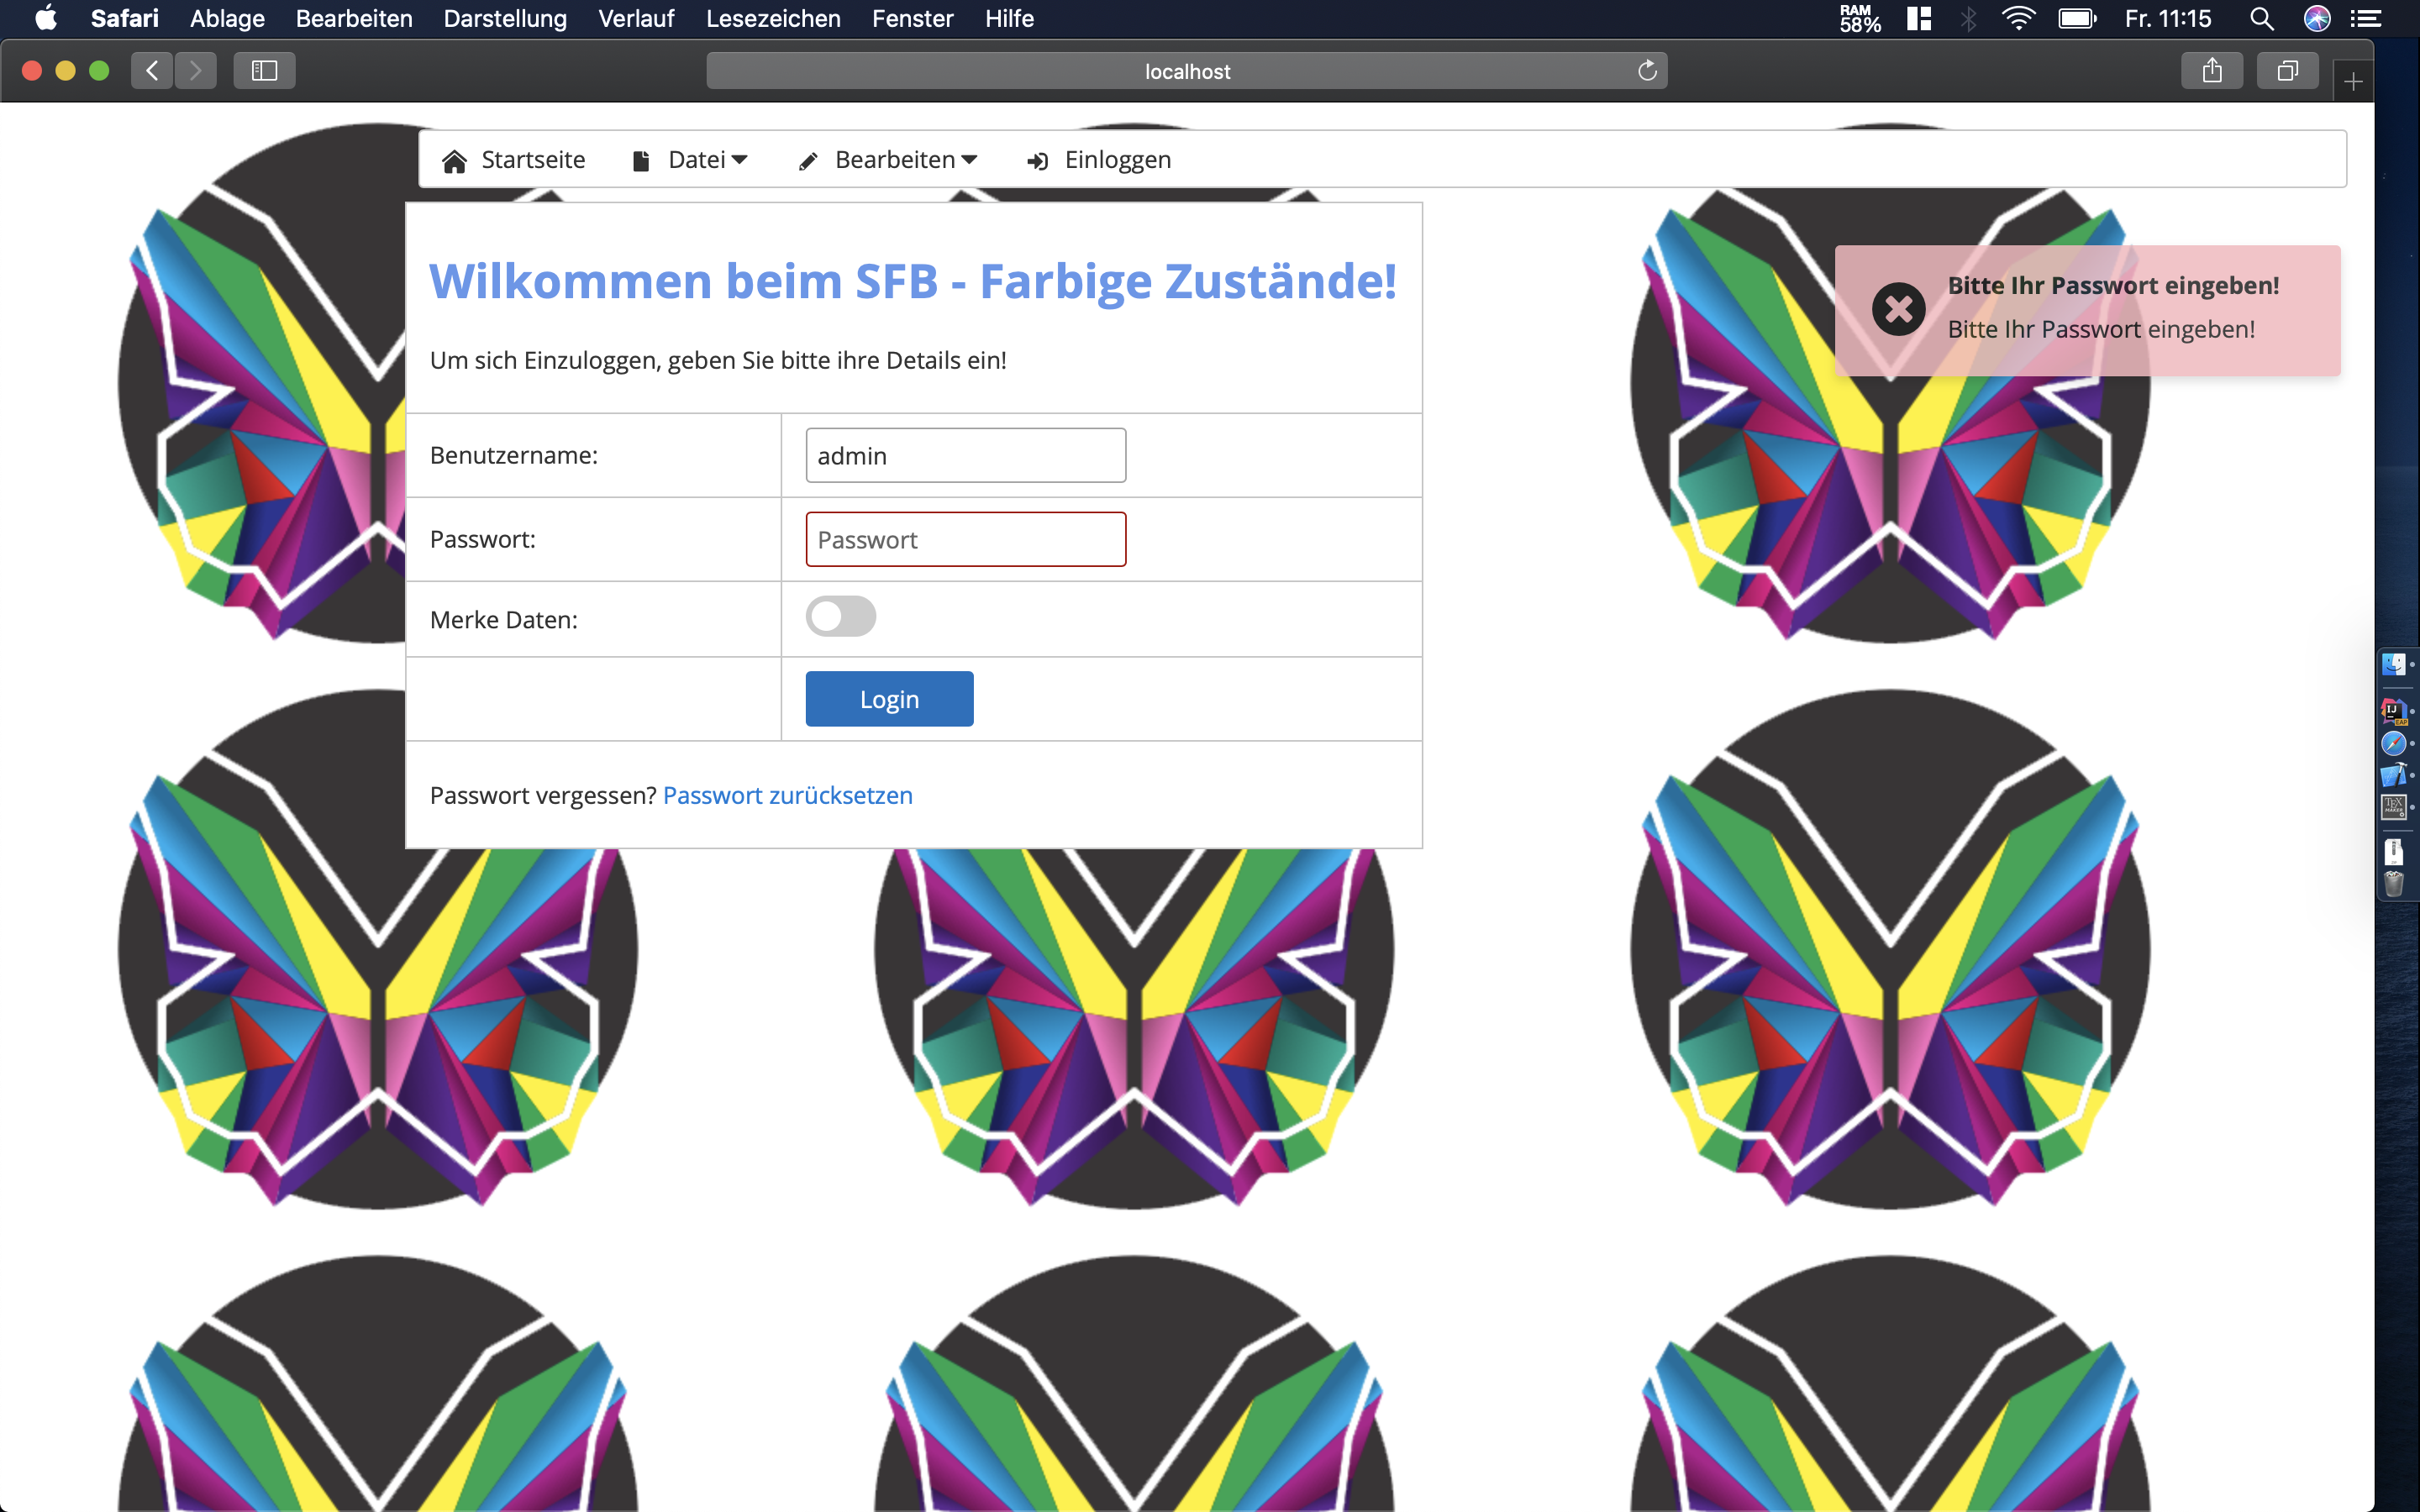
\includegraphics[width=1\textwidth]{Screenshots/311BittePasswordEingeben.png}
\textit{Abbildung 3.1.1.9: Fehlermeldung: Bitte Ihr Passwort eingeben!}
} \\

Wie man in den Beispielen sehen kann, kann man sich mit unterschiedlichen Benutzern einloggen, welche unterschiedliche den Rollen entsprechende Features haben. Man muss das richtige Passwort für den Benutzernamen eingeben, um sich einloggen zu können. Die Tests verliefen erfolgreich. \\ 

%%%%%

\subsubsection{Anwendungsfall: Seitenzugriff}

%
\paragraph{Nutzer versucht sich Zugang zu nicht authorisierten Seiten zu verschaffen:}

Ausgangssituation: Wir haben einen User \textit{tr}, welcher nur die Rolle Transporter zugewiesen hat. Dieser versucht nun von seiner Startseite aus über folgenden Link \textit{http://localhost:8080/admin/nutzerVerwaltung.xhtml} die Seite zum Verwalten der Nutzer zu erreichen. 

\hypertarget{sc3.1.2.1.1}{
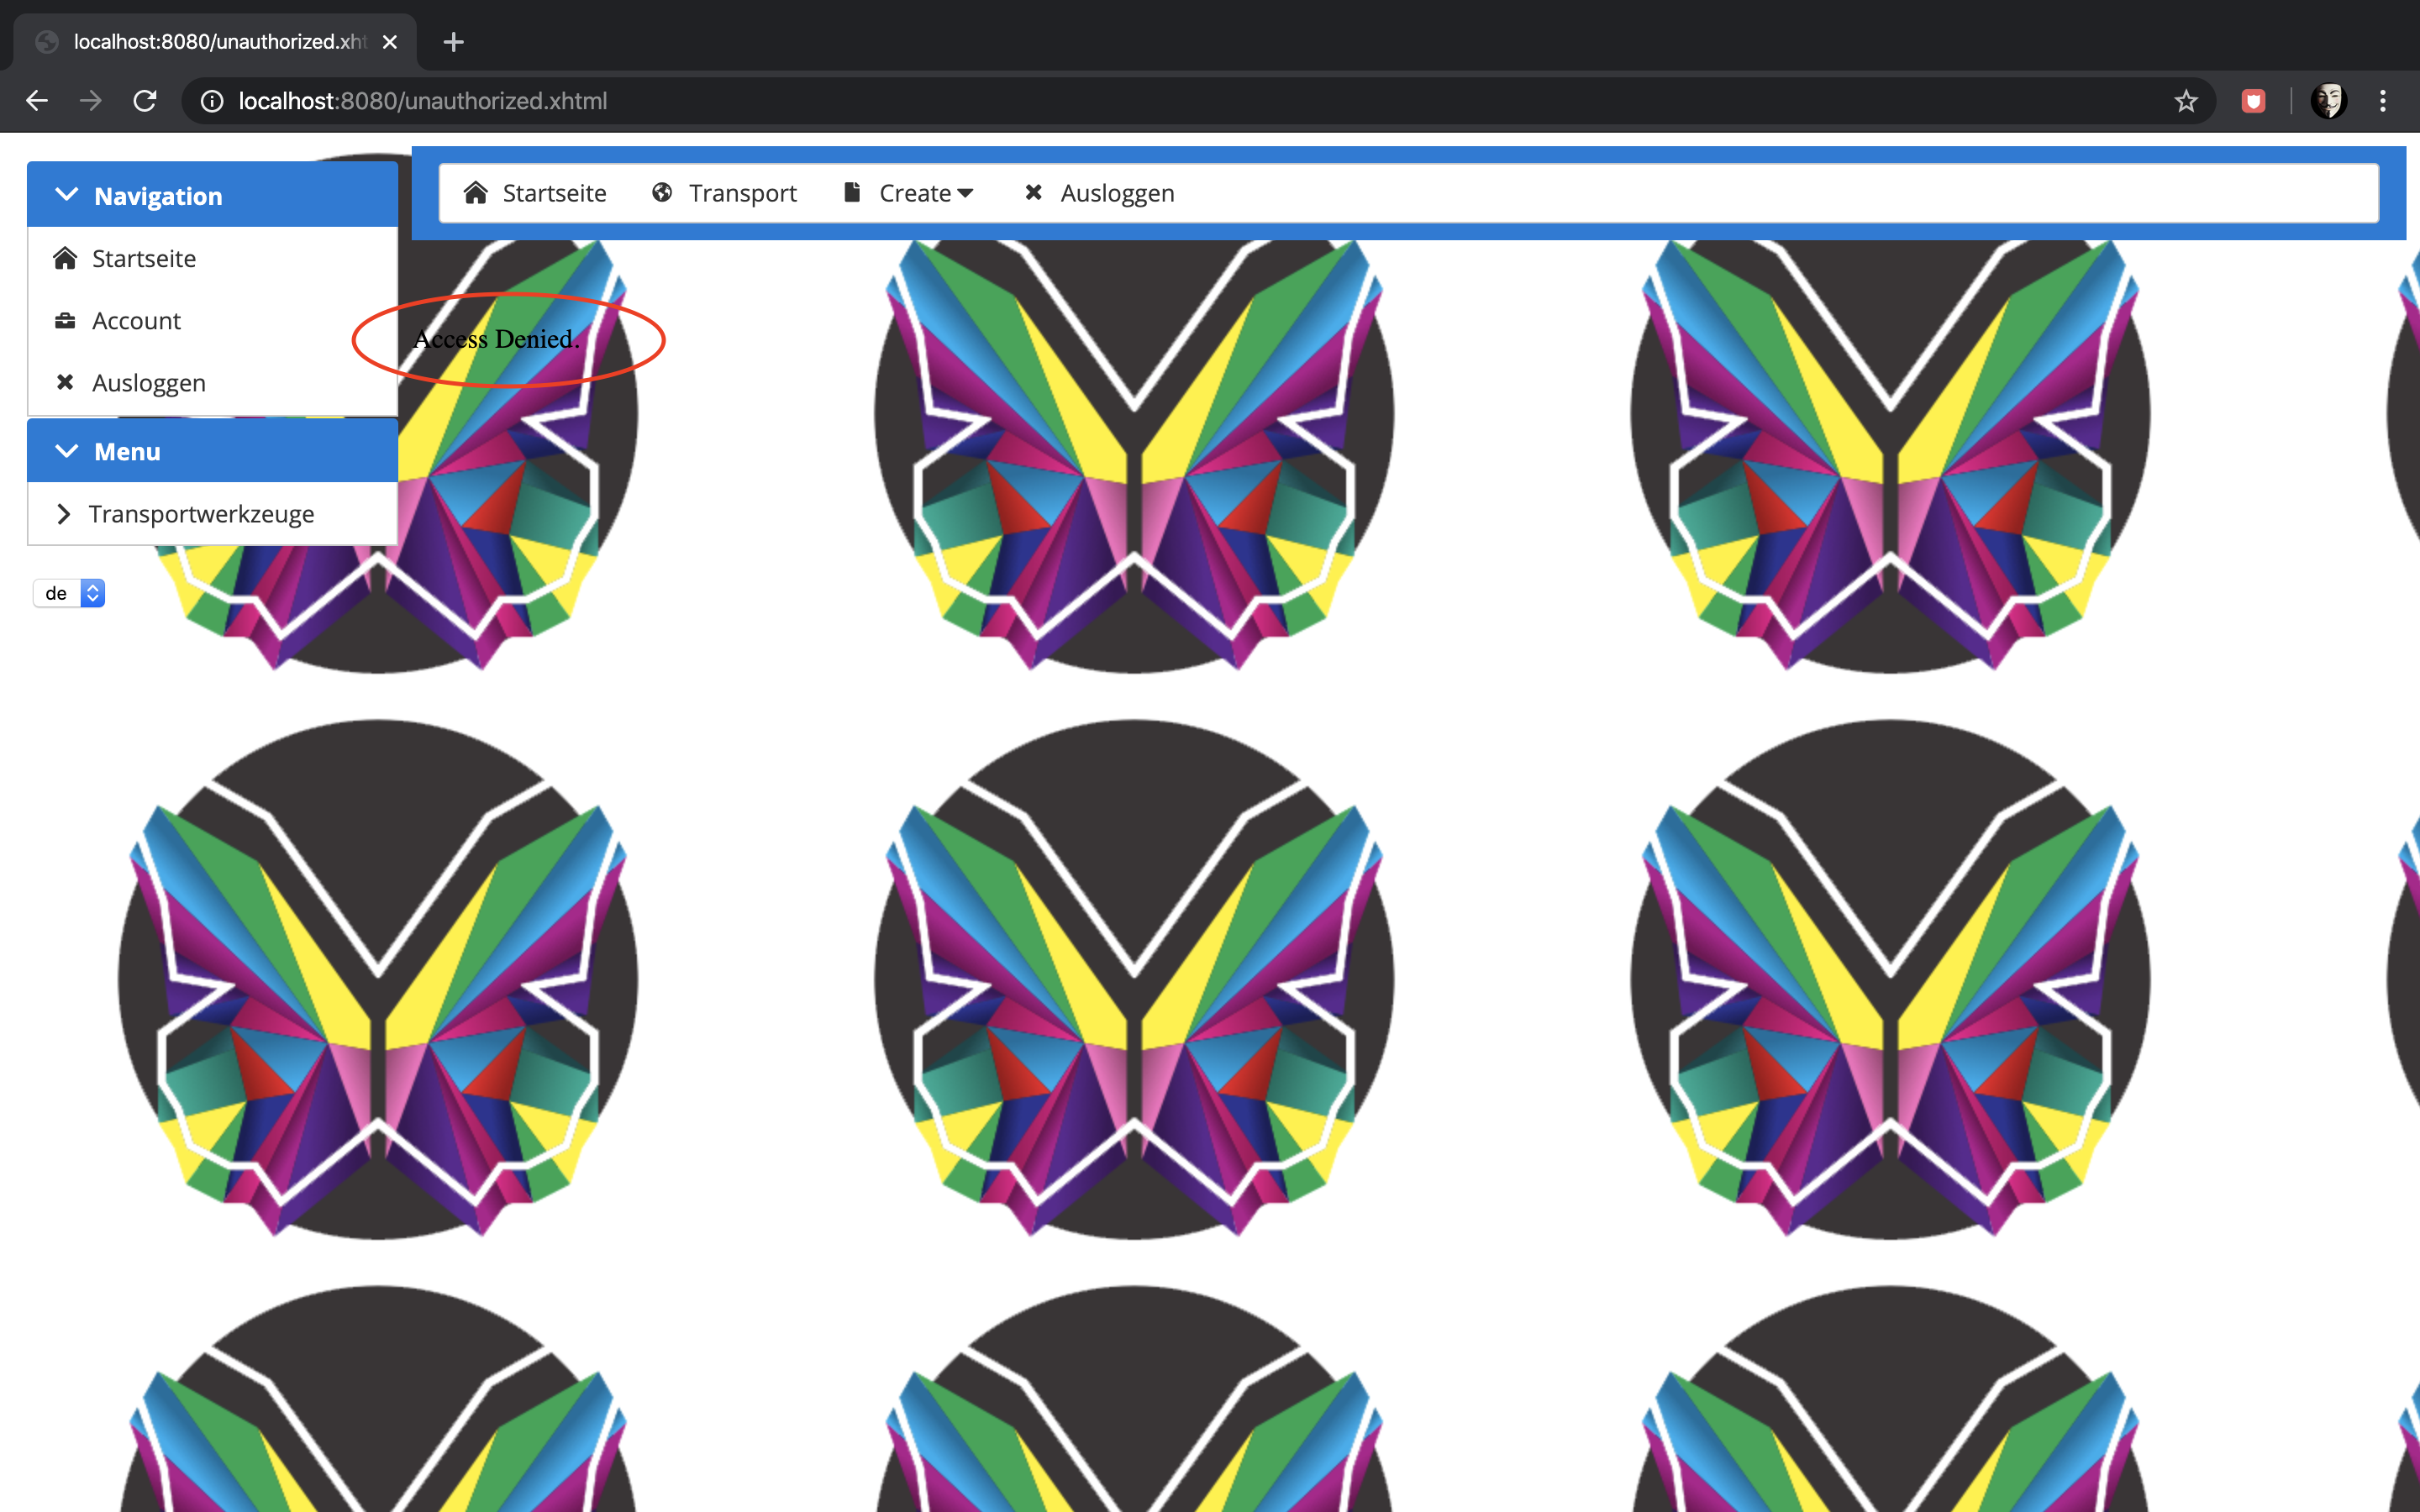
\includegraphics[width=1\textwidth]{Screenshots/3121.png}
\textit{Abbildung 3.1.2.1: Zugriff verweigert}
} \\

Man wird auf die \hyperlink{sc3.1.2.1.1}{Zugriff Verweigert} seite umgeleitet. Man kommt nicht auf die gewollte Seite des Administrators, da man keine Zugriffsrechte hat. 
Der Test verlief erfolgreich.

%
\paragraph{Nutzer verschafft sich Zugang zu authorisierten Seiten:}

Ausgangssituation: Wir haben einen User \textit{tr}, welcher nur die Rolle Transporter zugewiesen hat. Dieser versucht nun von seiner Startseite aus über folgenden Link \textit{http://localhost:8080/transport/probenVerlust.xhtml} die Seite zum Probenverlust melden zu erreichen. 

\hypertarget{sc3.1.2.2.1}{
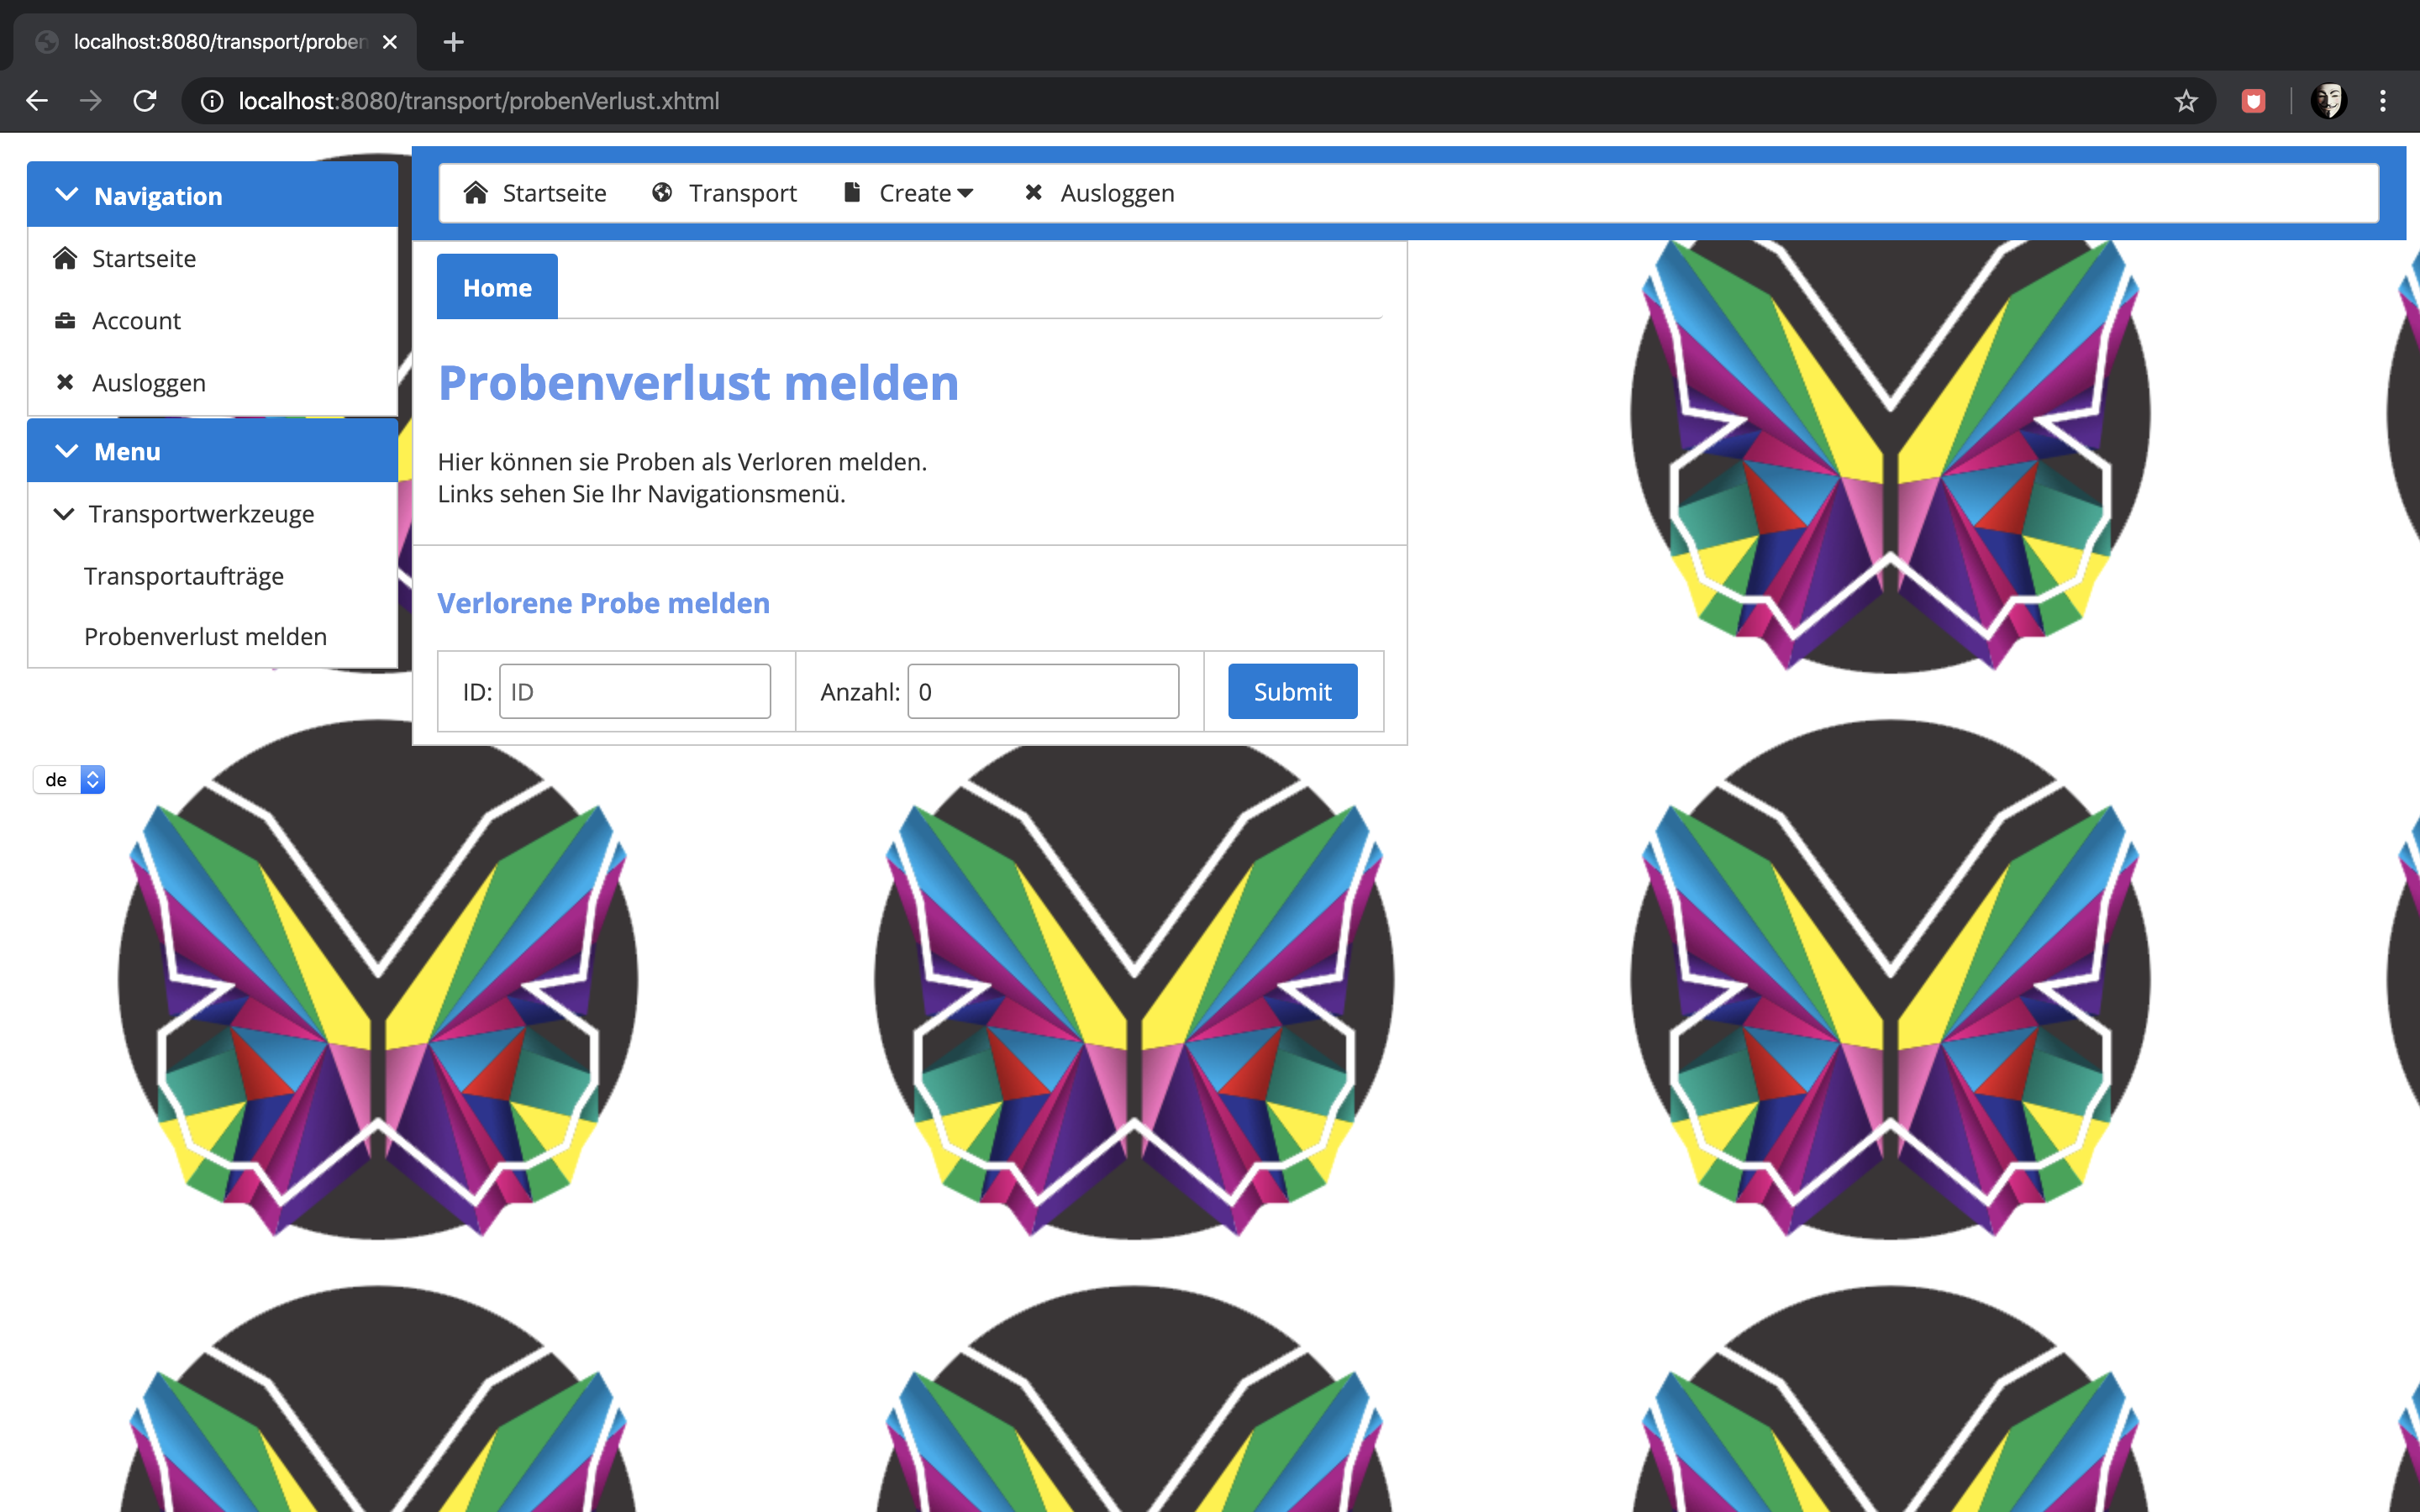
\includegraphics[width=1\textwidth]{Screenshots/3122.png}
\textit{Abbildung 3.1.2.2: Zugriff gewährt}
} \\

Der  \hyperlink{sc3.1.2.1.1}{Zugriff} zu der Seite wurde dem User gewährt, da er die richtige Rolle besitzt. Der Test verlief erfolgreich. 

%%%%%

\subsubsection{Ausloggen eines Benutzers}

Ein eingeloggter Benutzer, hier der \textit{admin} befindet sich auf einer \hyperlink{sc3.1.3.1.1}{beliebigen Seite} im System und möchte sich ausloggen. Hierfür drückt er oben den Ausloggen Button. 

\hypertarget{sc3.1.3.1.1}{
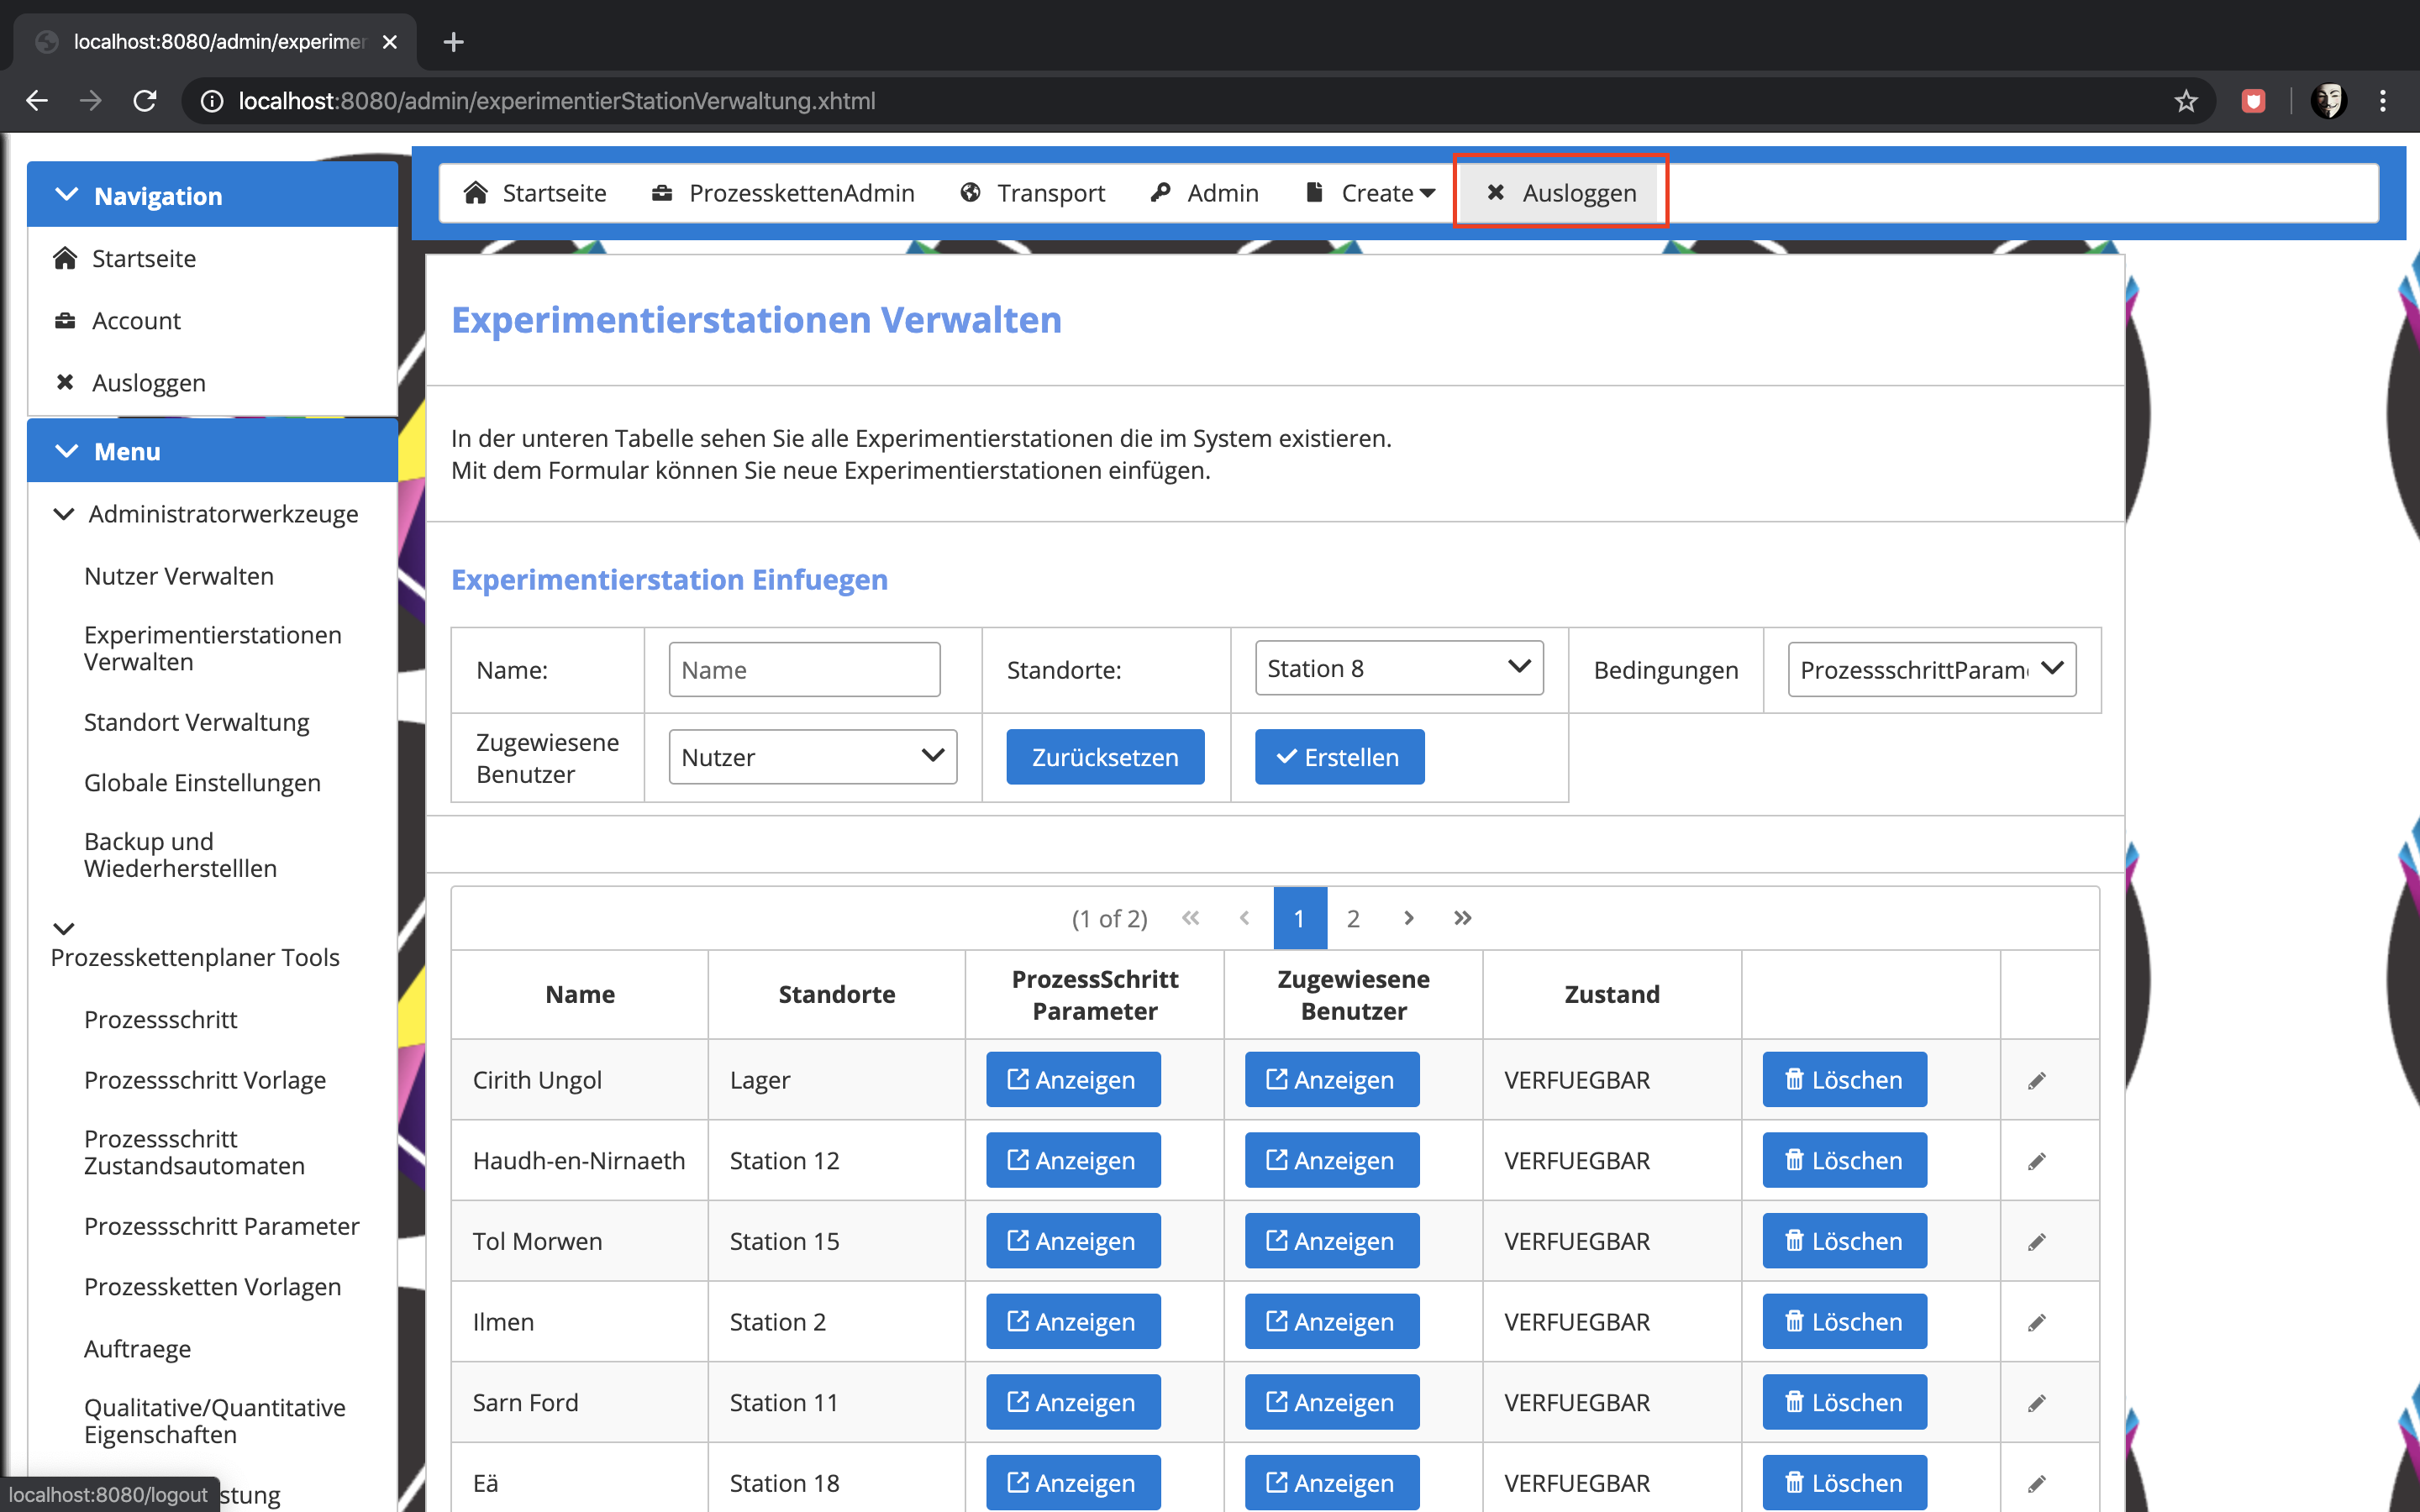
\includegraphics[width=1\textwidth]{Screenshots/31131.png}
\textit{Abbildung 3.1.3.1: Beliebige Seite mit Ausloggen Button markiert}
} \\

Er gelangt auf die Startseite und kann sich neu anmelden. Der Test war erfolgreich. 

\hypertarget{sc3.1.3.2.1}{
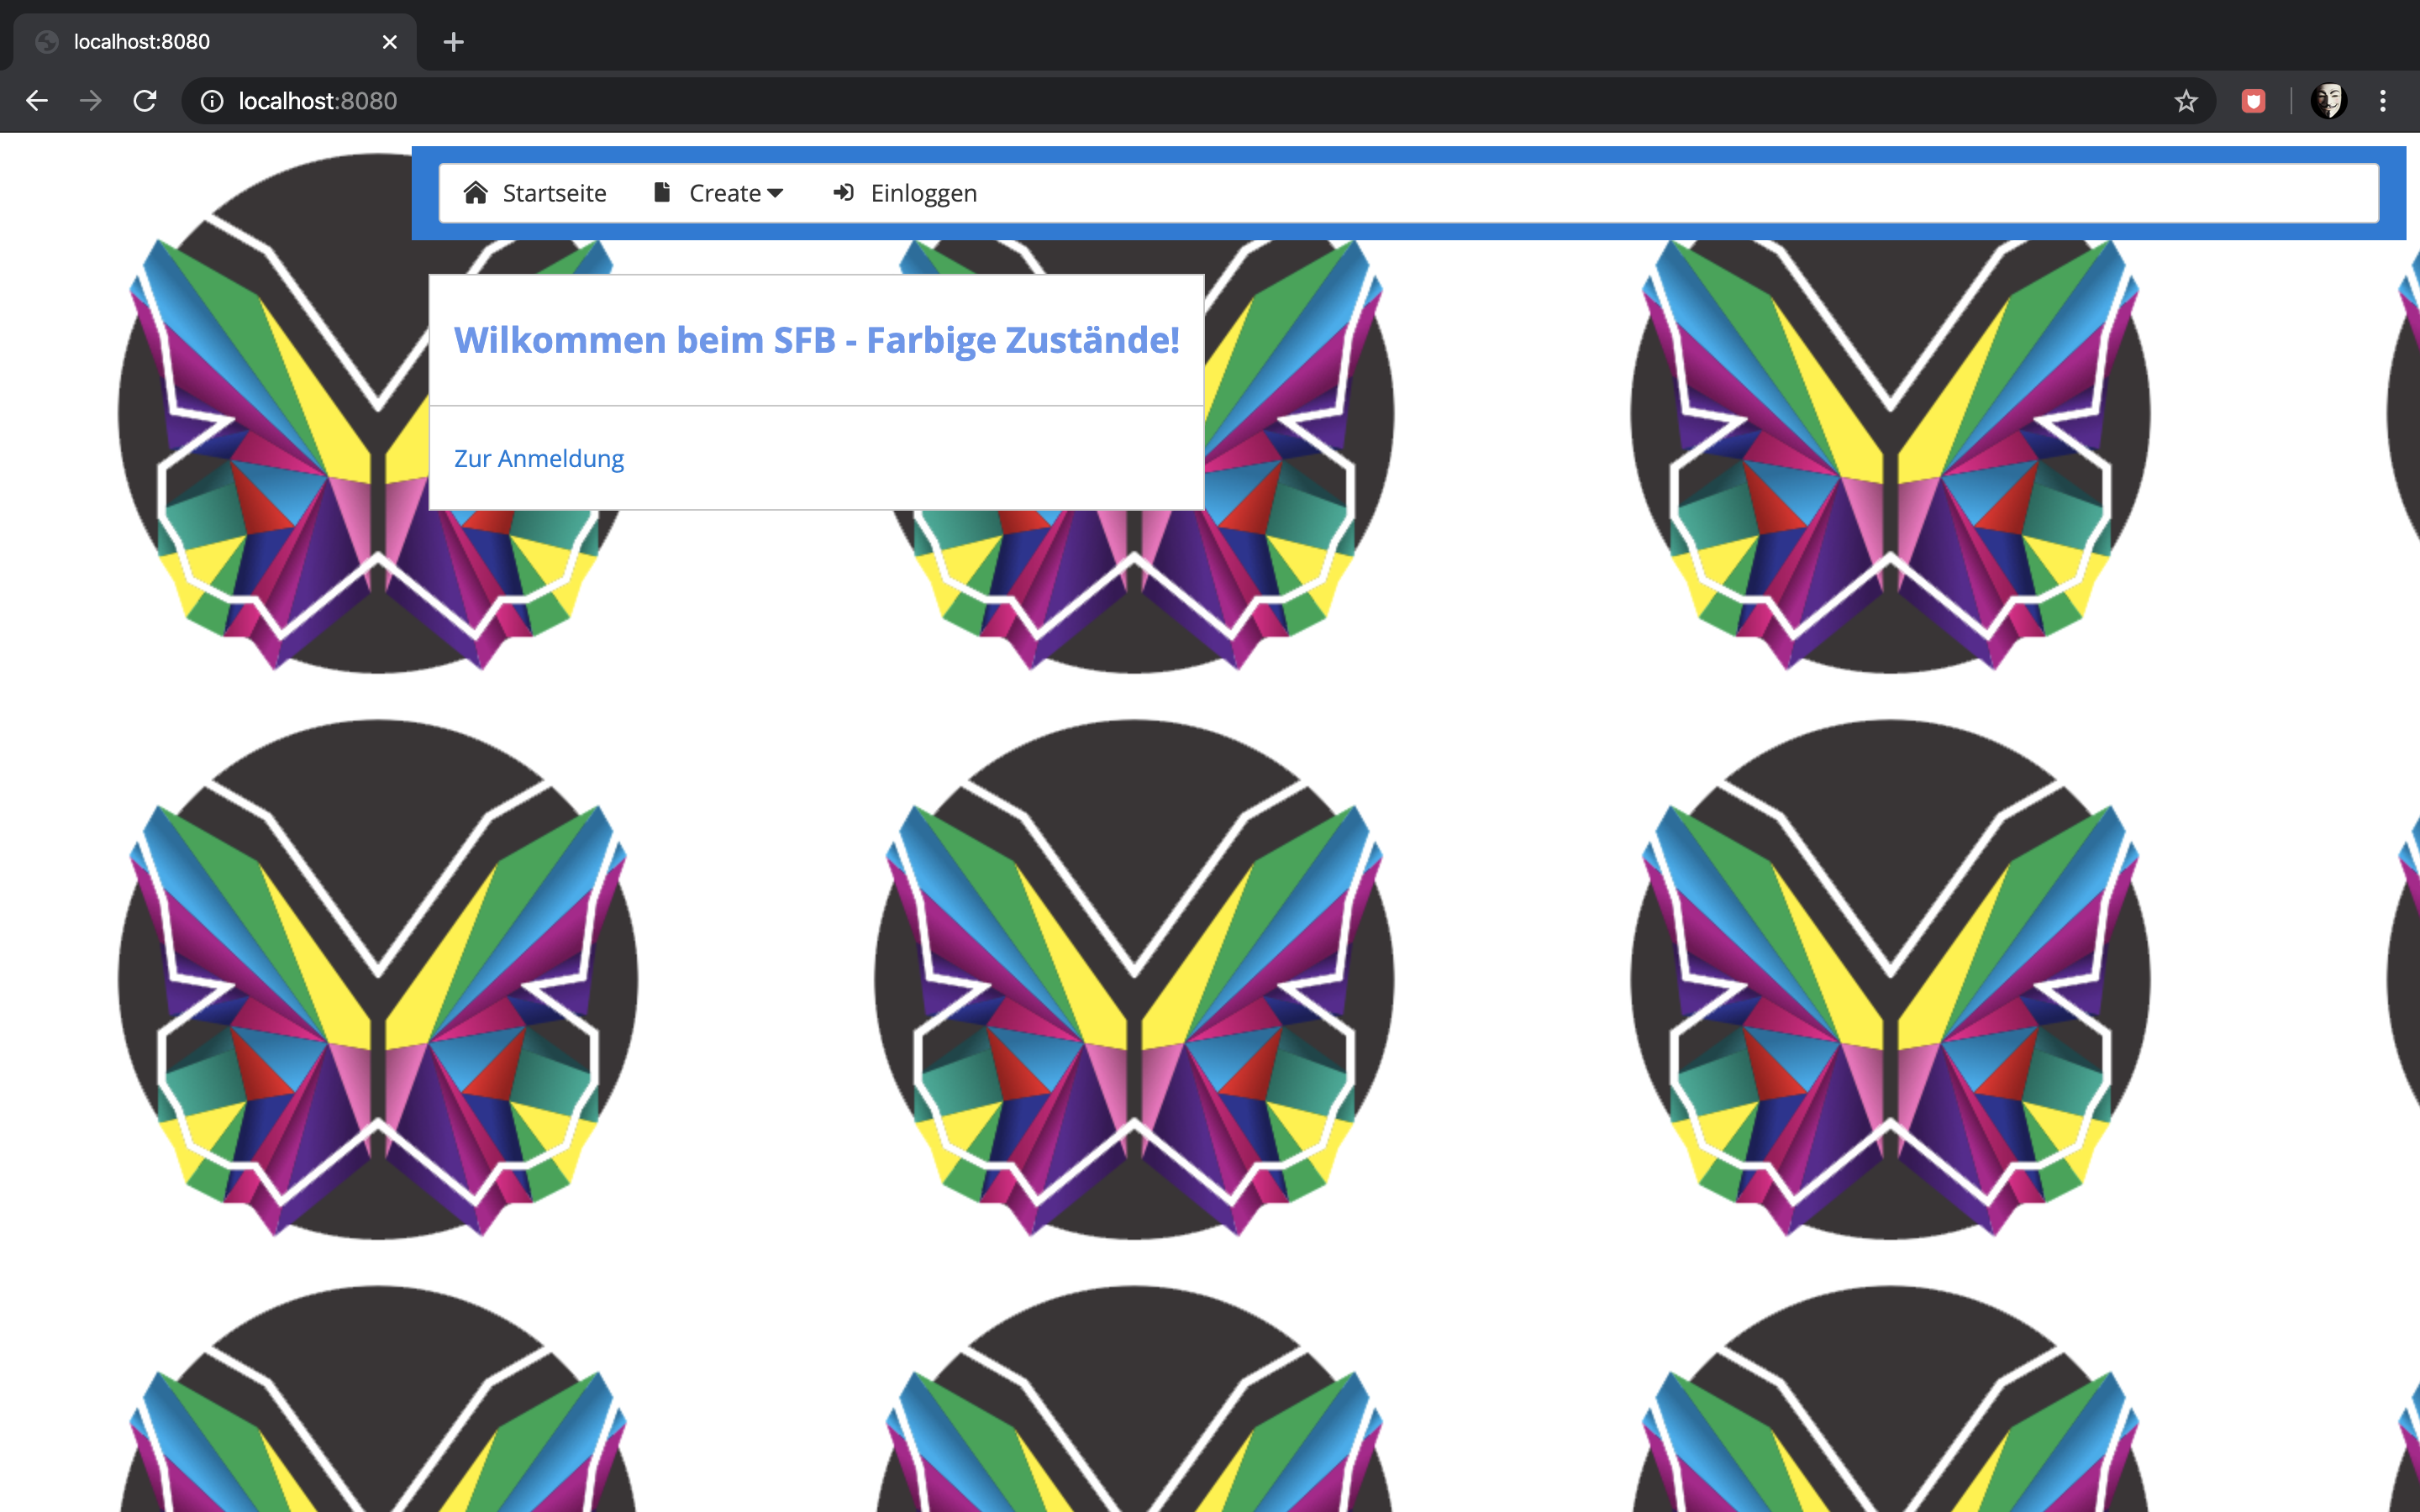
\includegraphics[width=1\textwidth]{Screenshots/31132.png}
\textit{Abbildung 3.1.3.2: Startseite}
} \\

%%%%%

\subsubsection{Sprache der Website ändern}

\paragraph{Von Deutsch zu Englisch}

Ein beliebiger Benutzer, hier der Nutzer \textit{admin} befindet sich auf einer beliebigen Seite des Systems. Die Ausgangssprache ist Deutsch und diese ist auch im \hyperlink{sc3.1.4.1.1}{User} gespeichert.  Er stellt unten links die gewünschte Sprache ein und sie wird umgestellt. 

\hypertarget{sc3.1.4.1.1}{
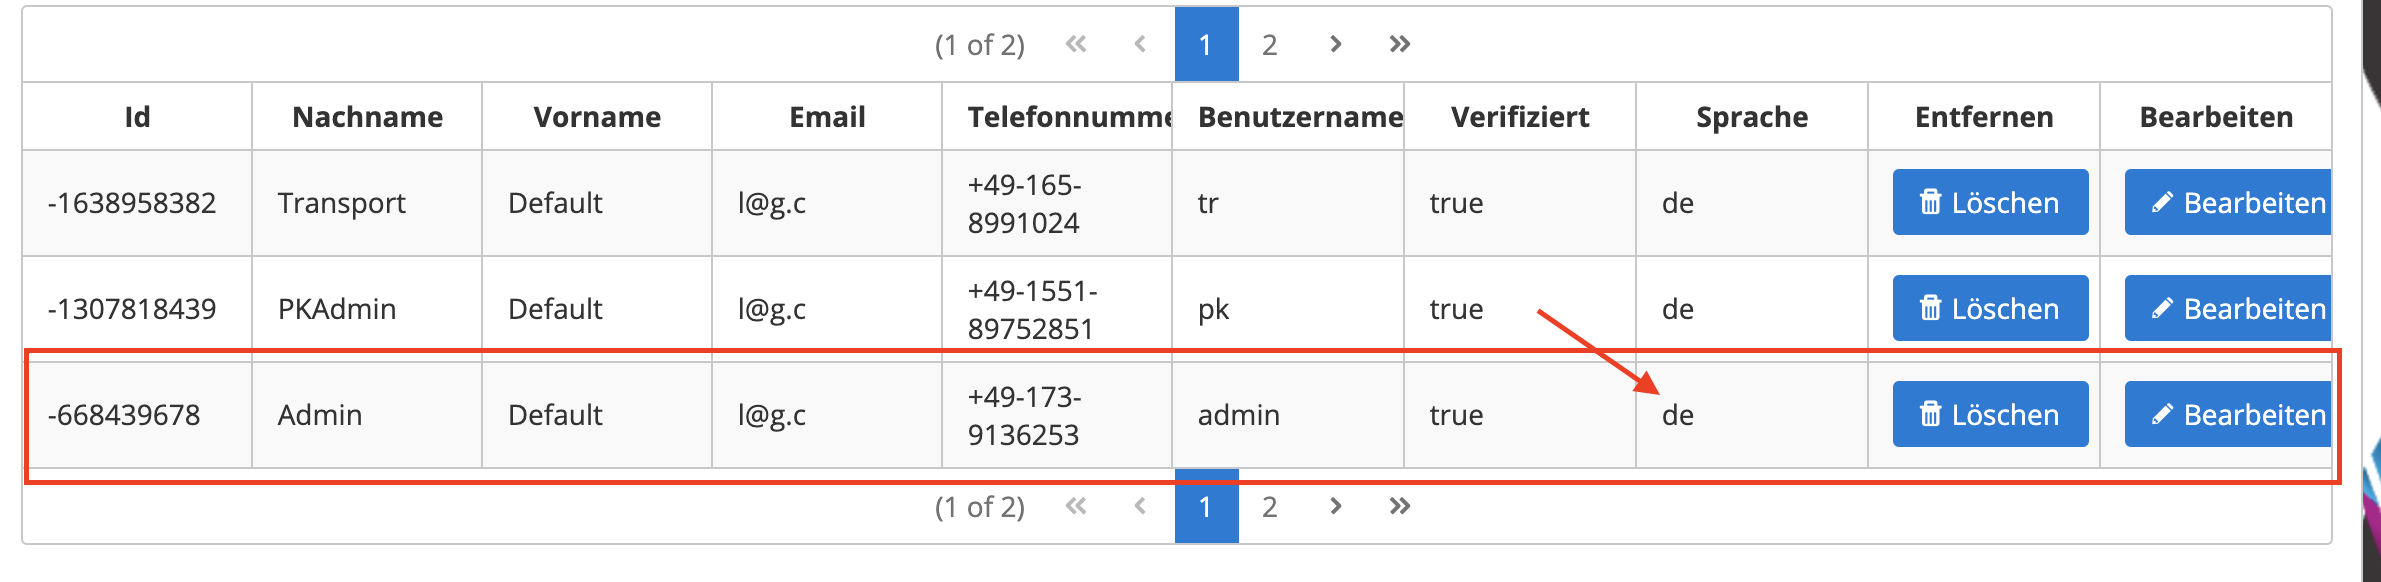
\includegraphics[width=1\textwidth]{Screenshots/31141.png}
\textit{Abbildung 3.1.4.1: Im Benutzer ist die Sprache Deutsch gespeichert und die Seite ist auf deutsch}
} \\

Die Sprache der Seite ist auf Englisch umgestellt und im User wurde die Sprache auf Englisch umgestellt. Somit wird bei jedem Reload einer Seite die gespeicherte Sprache angezeigt. 

\hypertarget{sc3.1.4.2.1}{
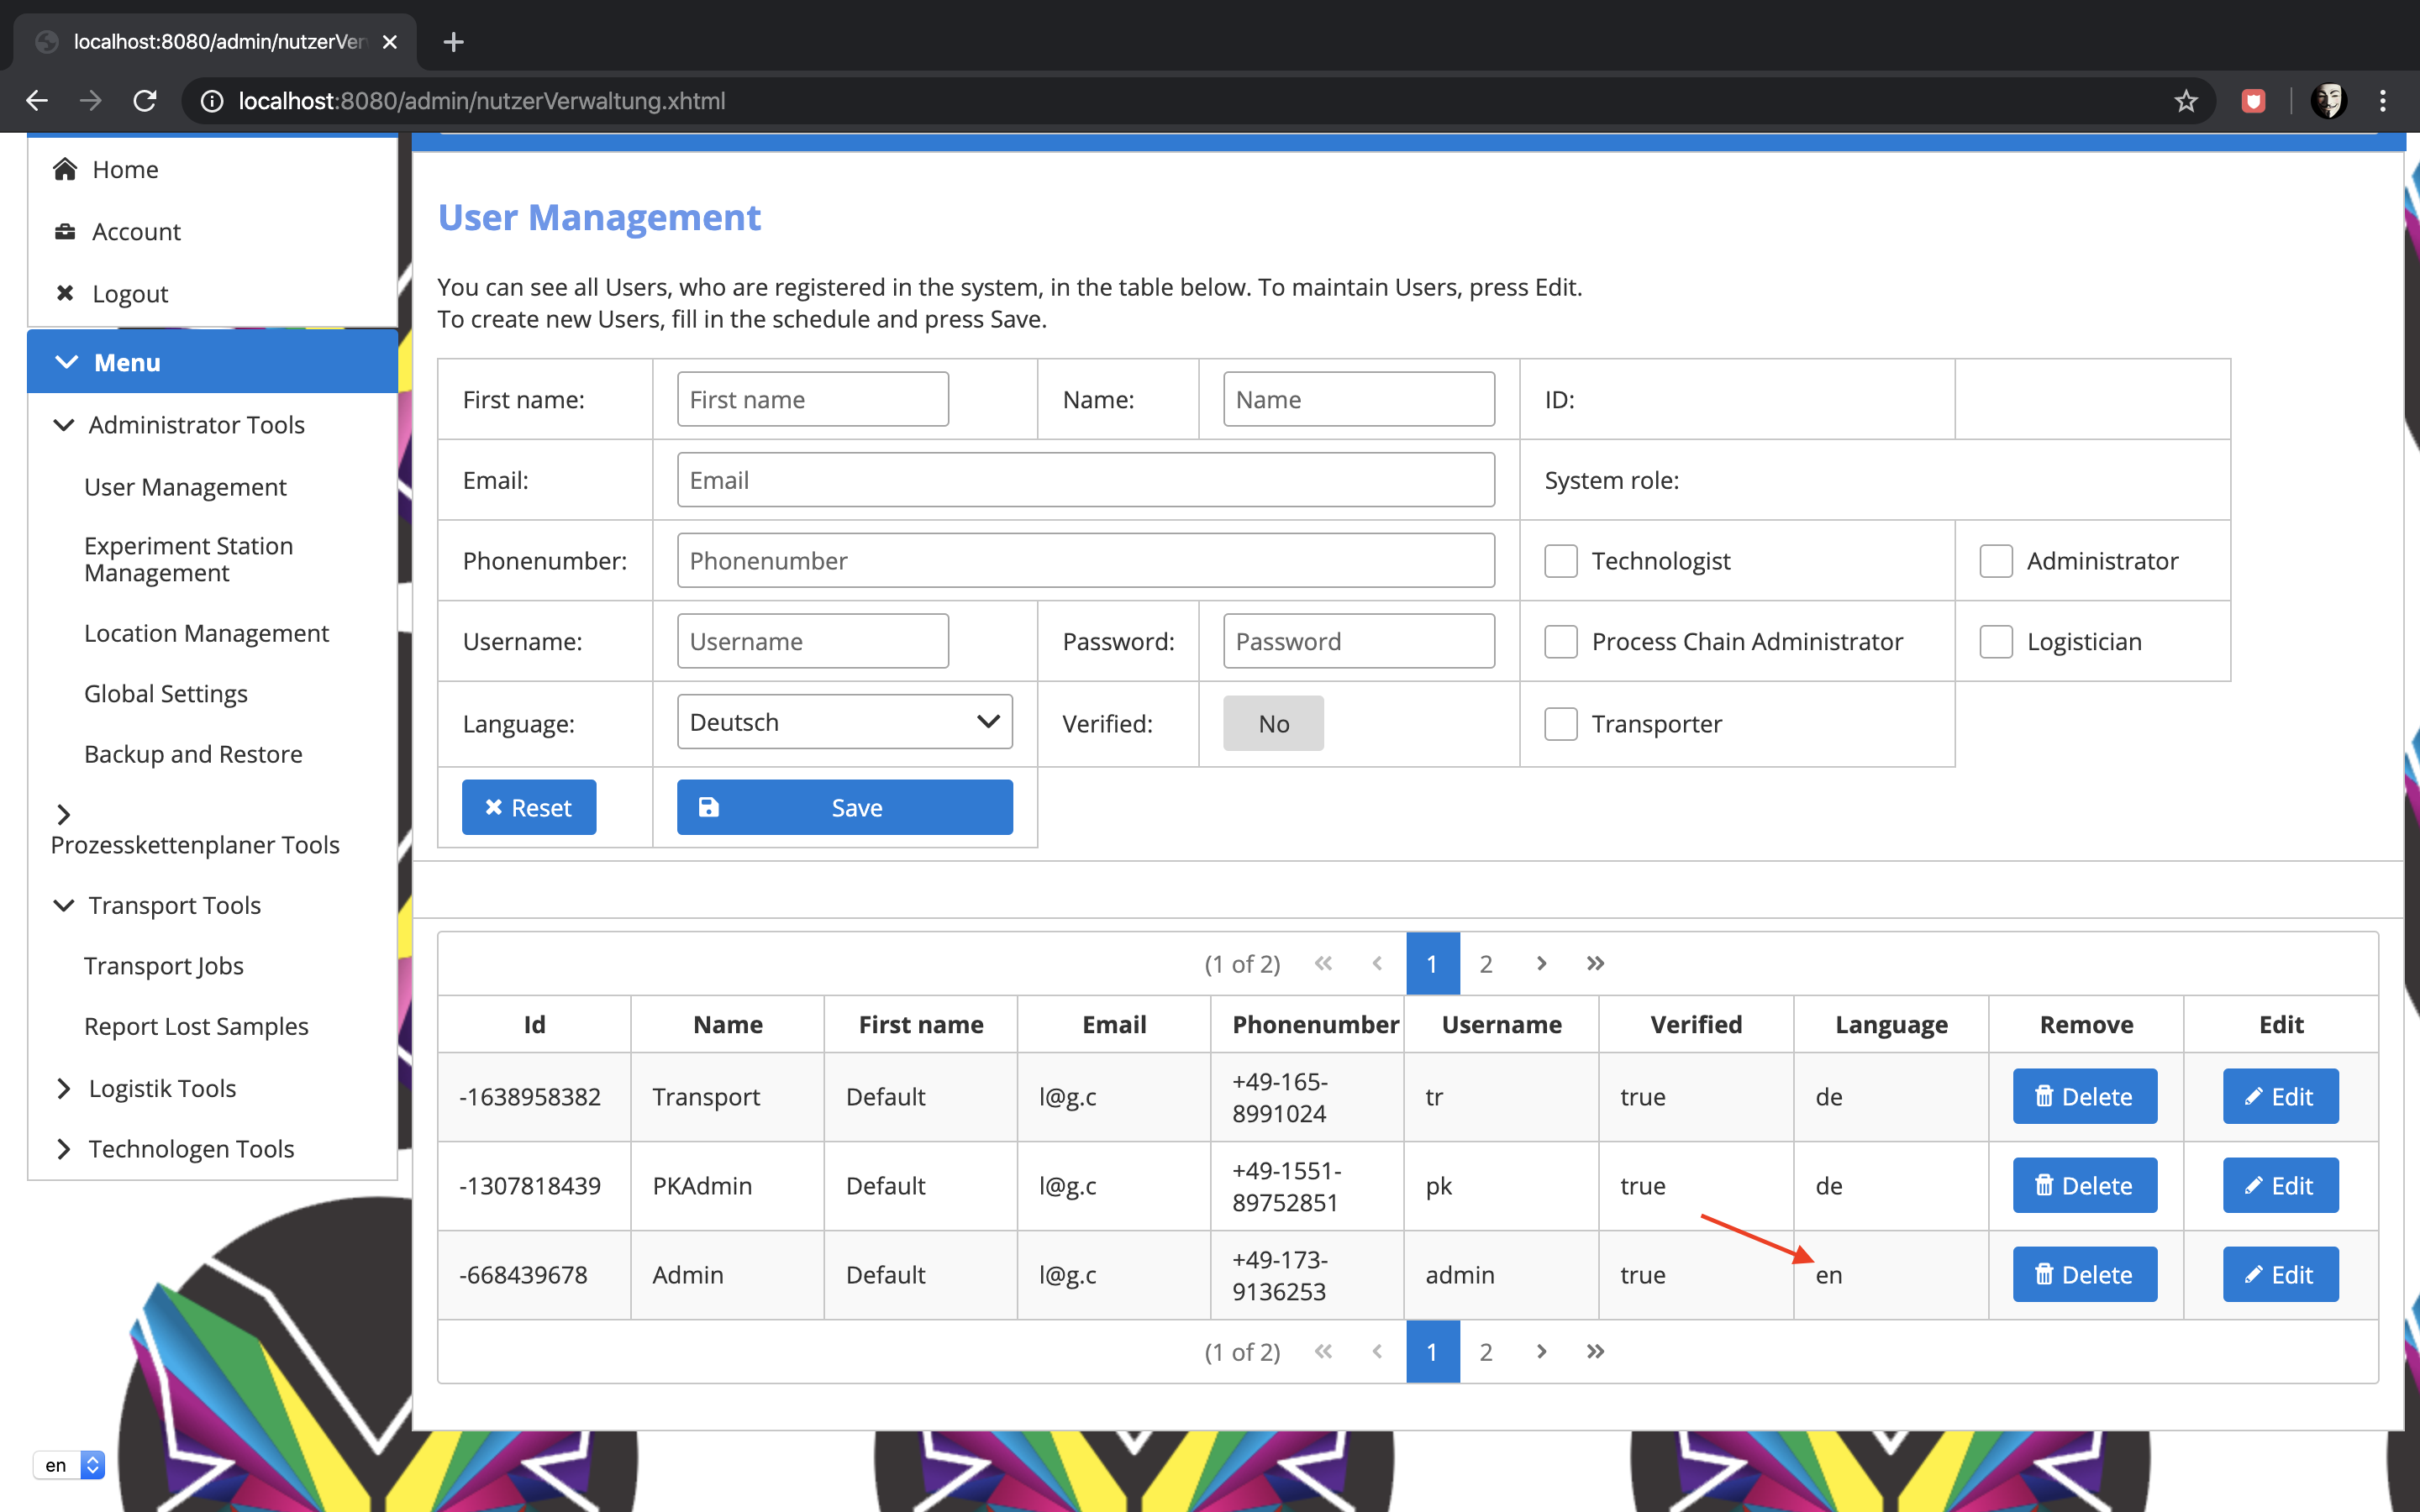
\includegraphics[width=1\textwidth]{Screenshots/31142.png}
\textit{Abbildung 3.1.4.2: Im Benutzer ist die Sprache Englisch gespeichert und die Seite ist auf englisch}
} \\

Der Test war erfolgreich. 

\paragraph{Von Englisch zu Deutsch}

Der Test wurde analog zu dem Von Deutsch zu Englisch ausgeführt. Ausgangssprache ist Englisch und es soll für den Nutzer die Sprache Deutsch eingestellt werden. Der Test verlief ebenfalls erfolgreich. Die Seite wird wieder auf \hyperlink{sc3.1.4.3.1}{deutsch} angezeigt.

\hypertarget{sc3.1.4.3.1}{
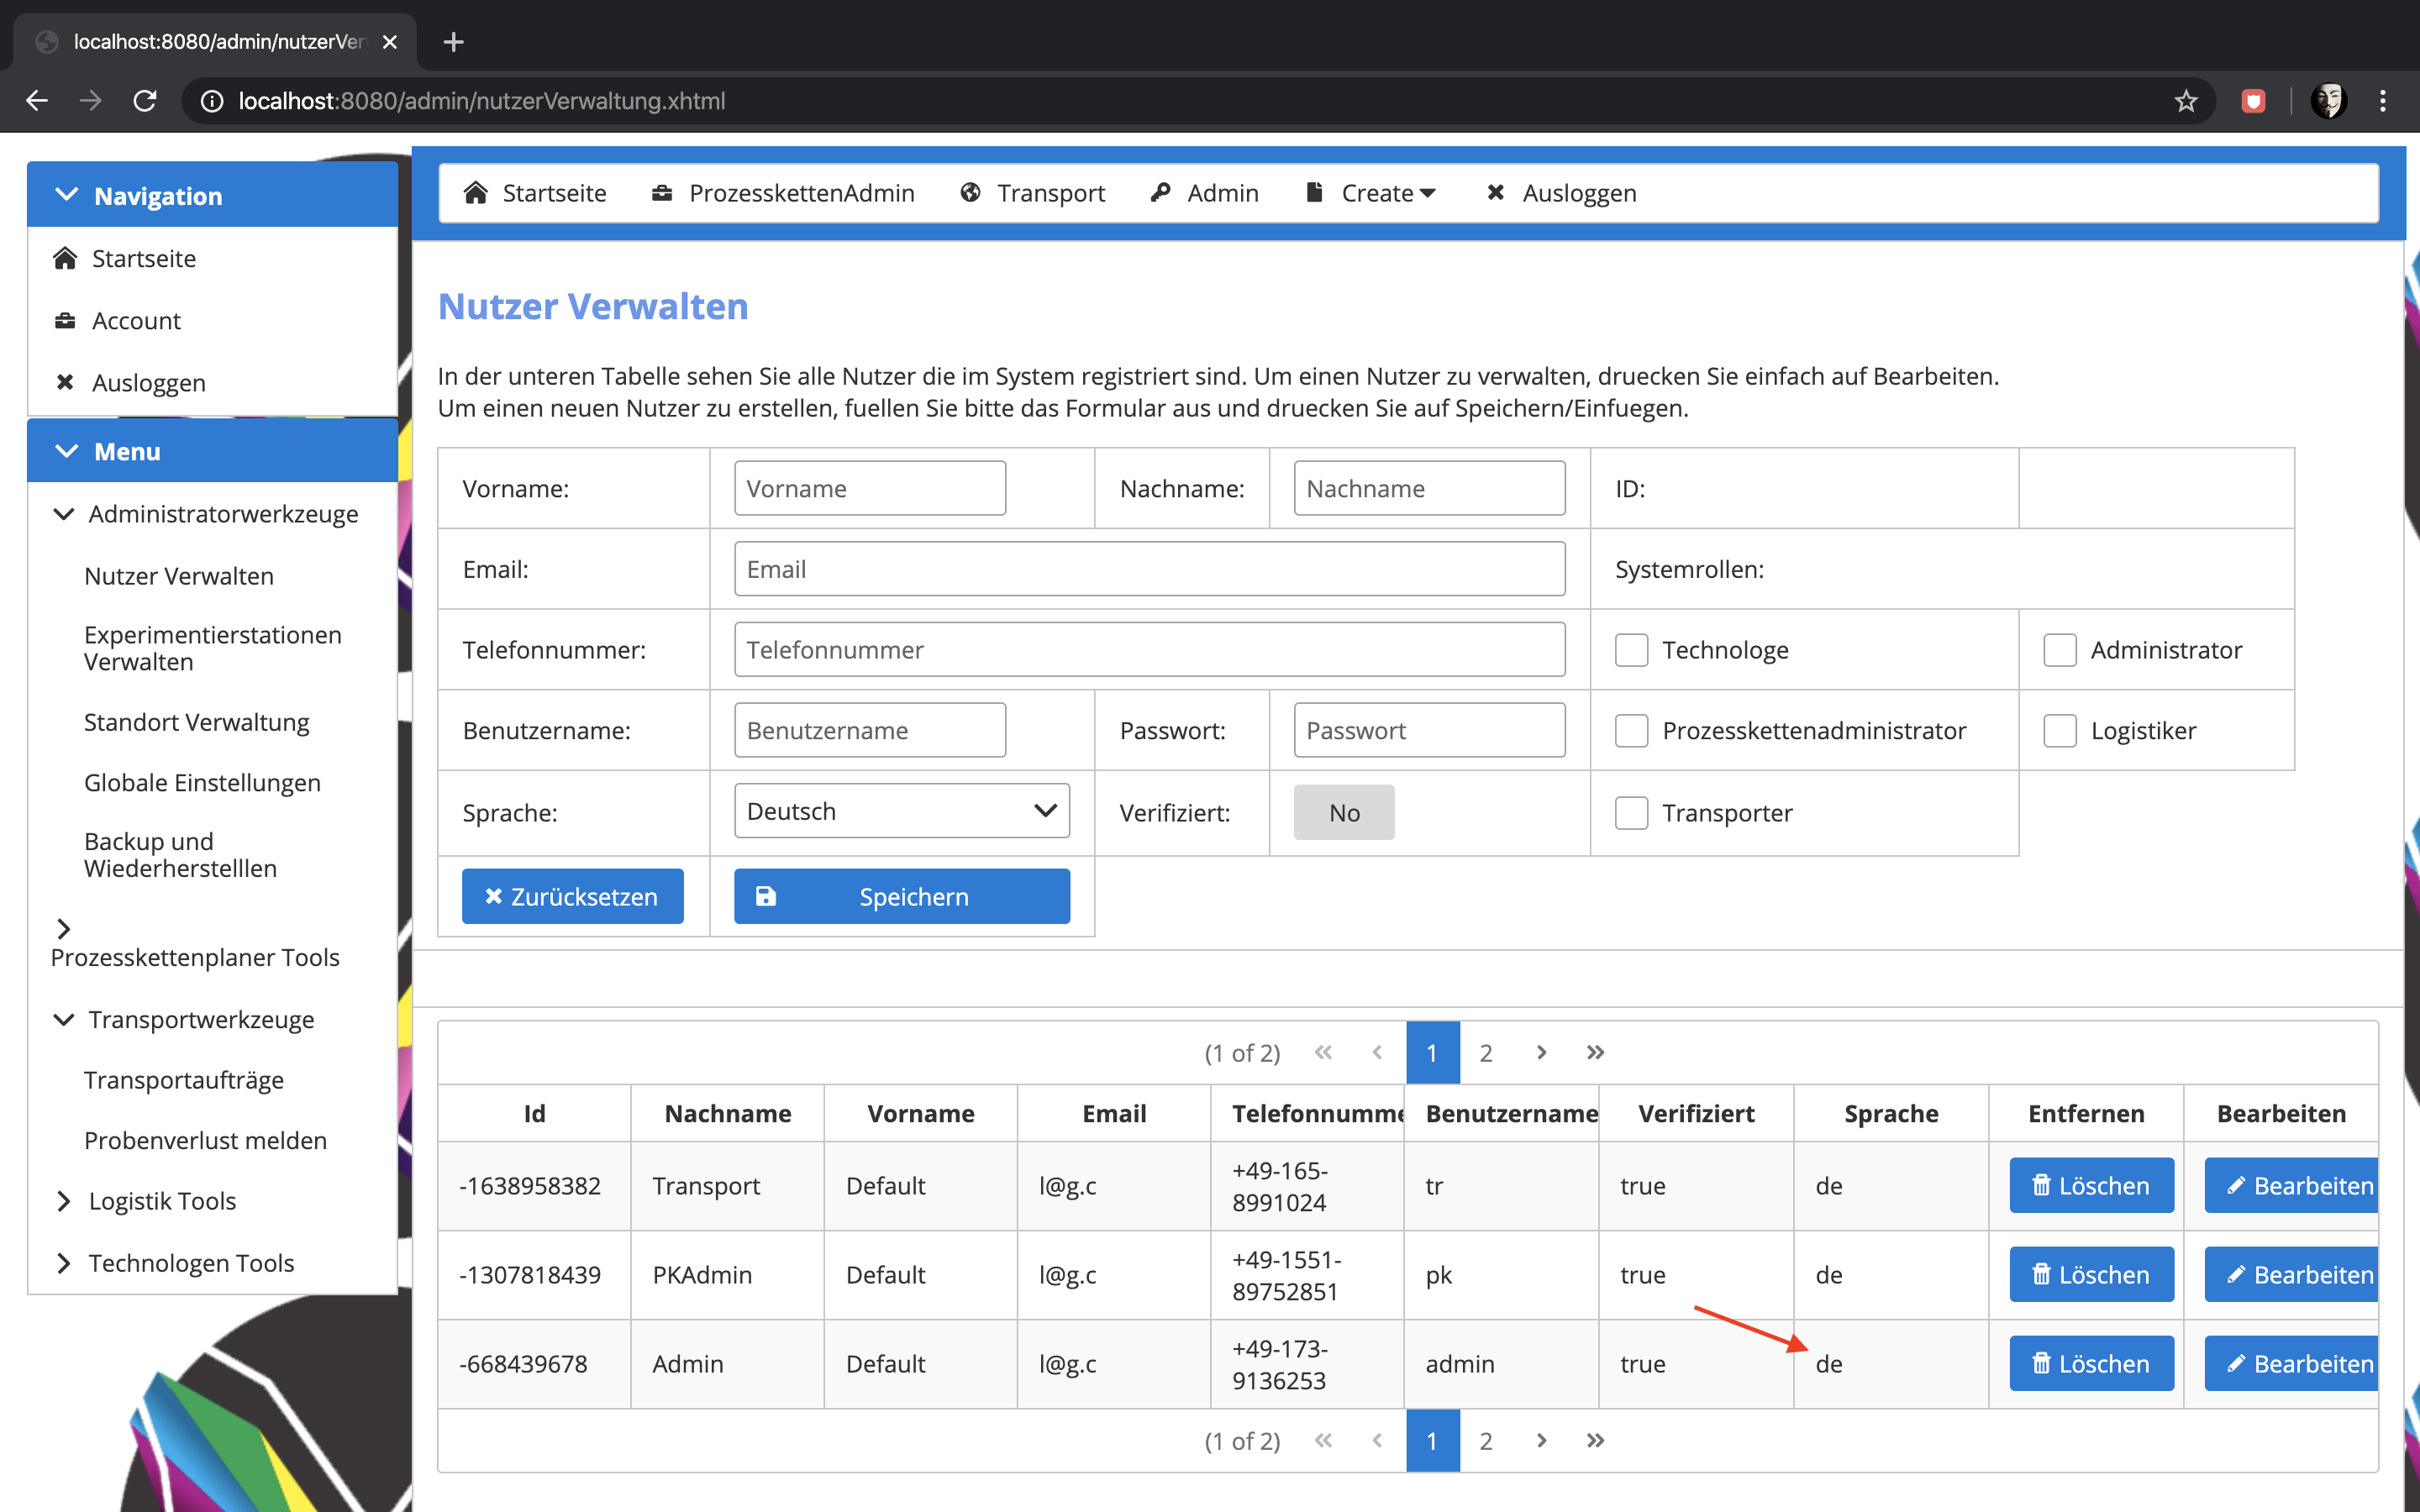
\includegraphics[width=1\textwidth]{Screenshots/31143.png}
\textit{Abbildung 3.1.4.3: Im Benutzer ist die Sprache Deutsch gespeichert und die Seite ist auf deutsch}
} \\

%%%%%

\subsubsection{}

%%%%%%%%%%%%%%

\subsection{Tests zum Administrator}

\subsubsection{Anwendungsfall: Beispiel 2}
Für die Erstellung und Kontrolle der Benutzer verfügt der Administrator über eine Tabelle und ein Formular.

Um einen neuen Benutzer zu erstellen, muss der Administrator die erforderlichen Felder in das Formular eingeben. Der Administrator muss versuchen, die Daten ordnungsgemäß einzugeben, damit die Erstellung erfolgreich ist.

\hypertarget{sc3.1.2.1}{
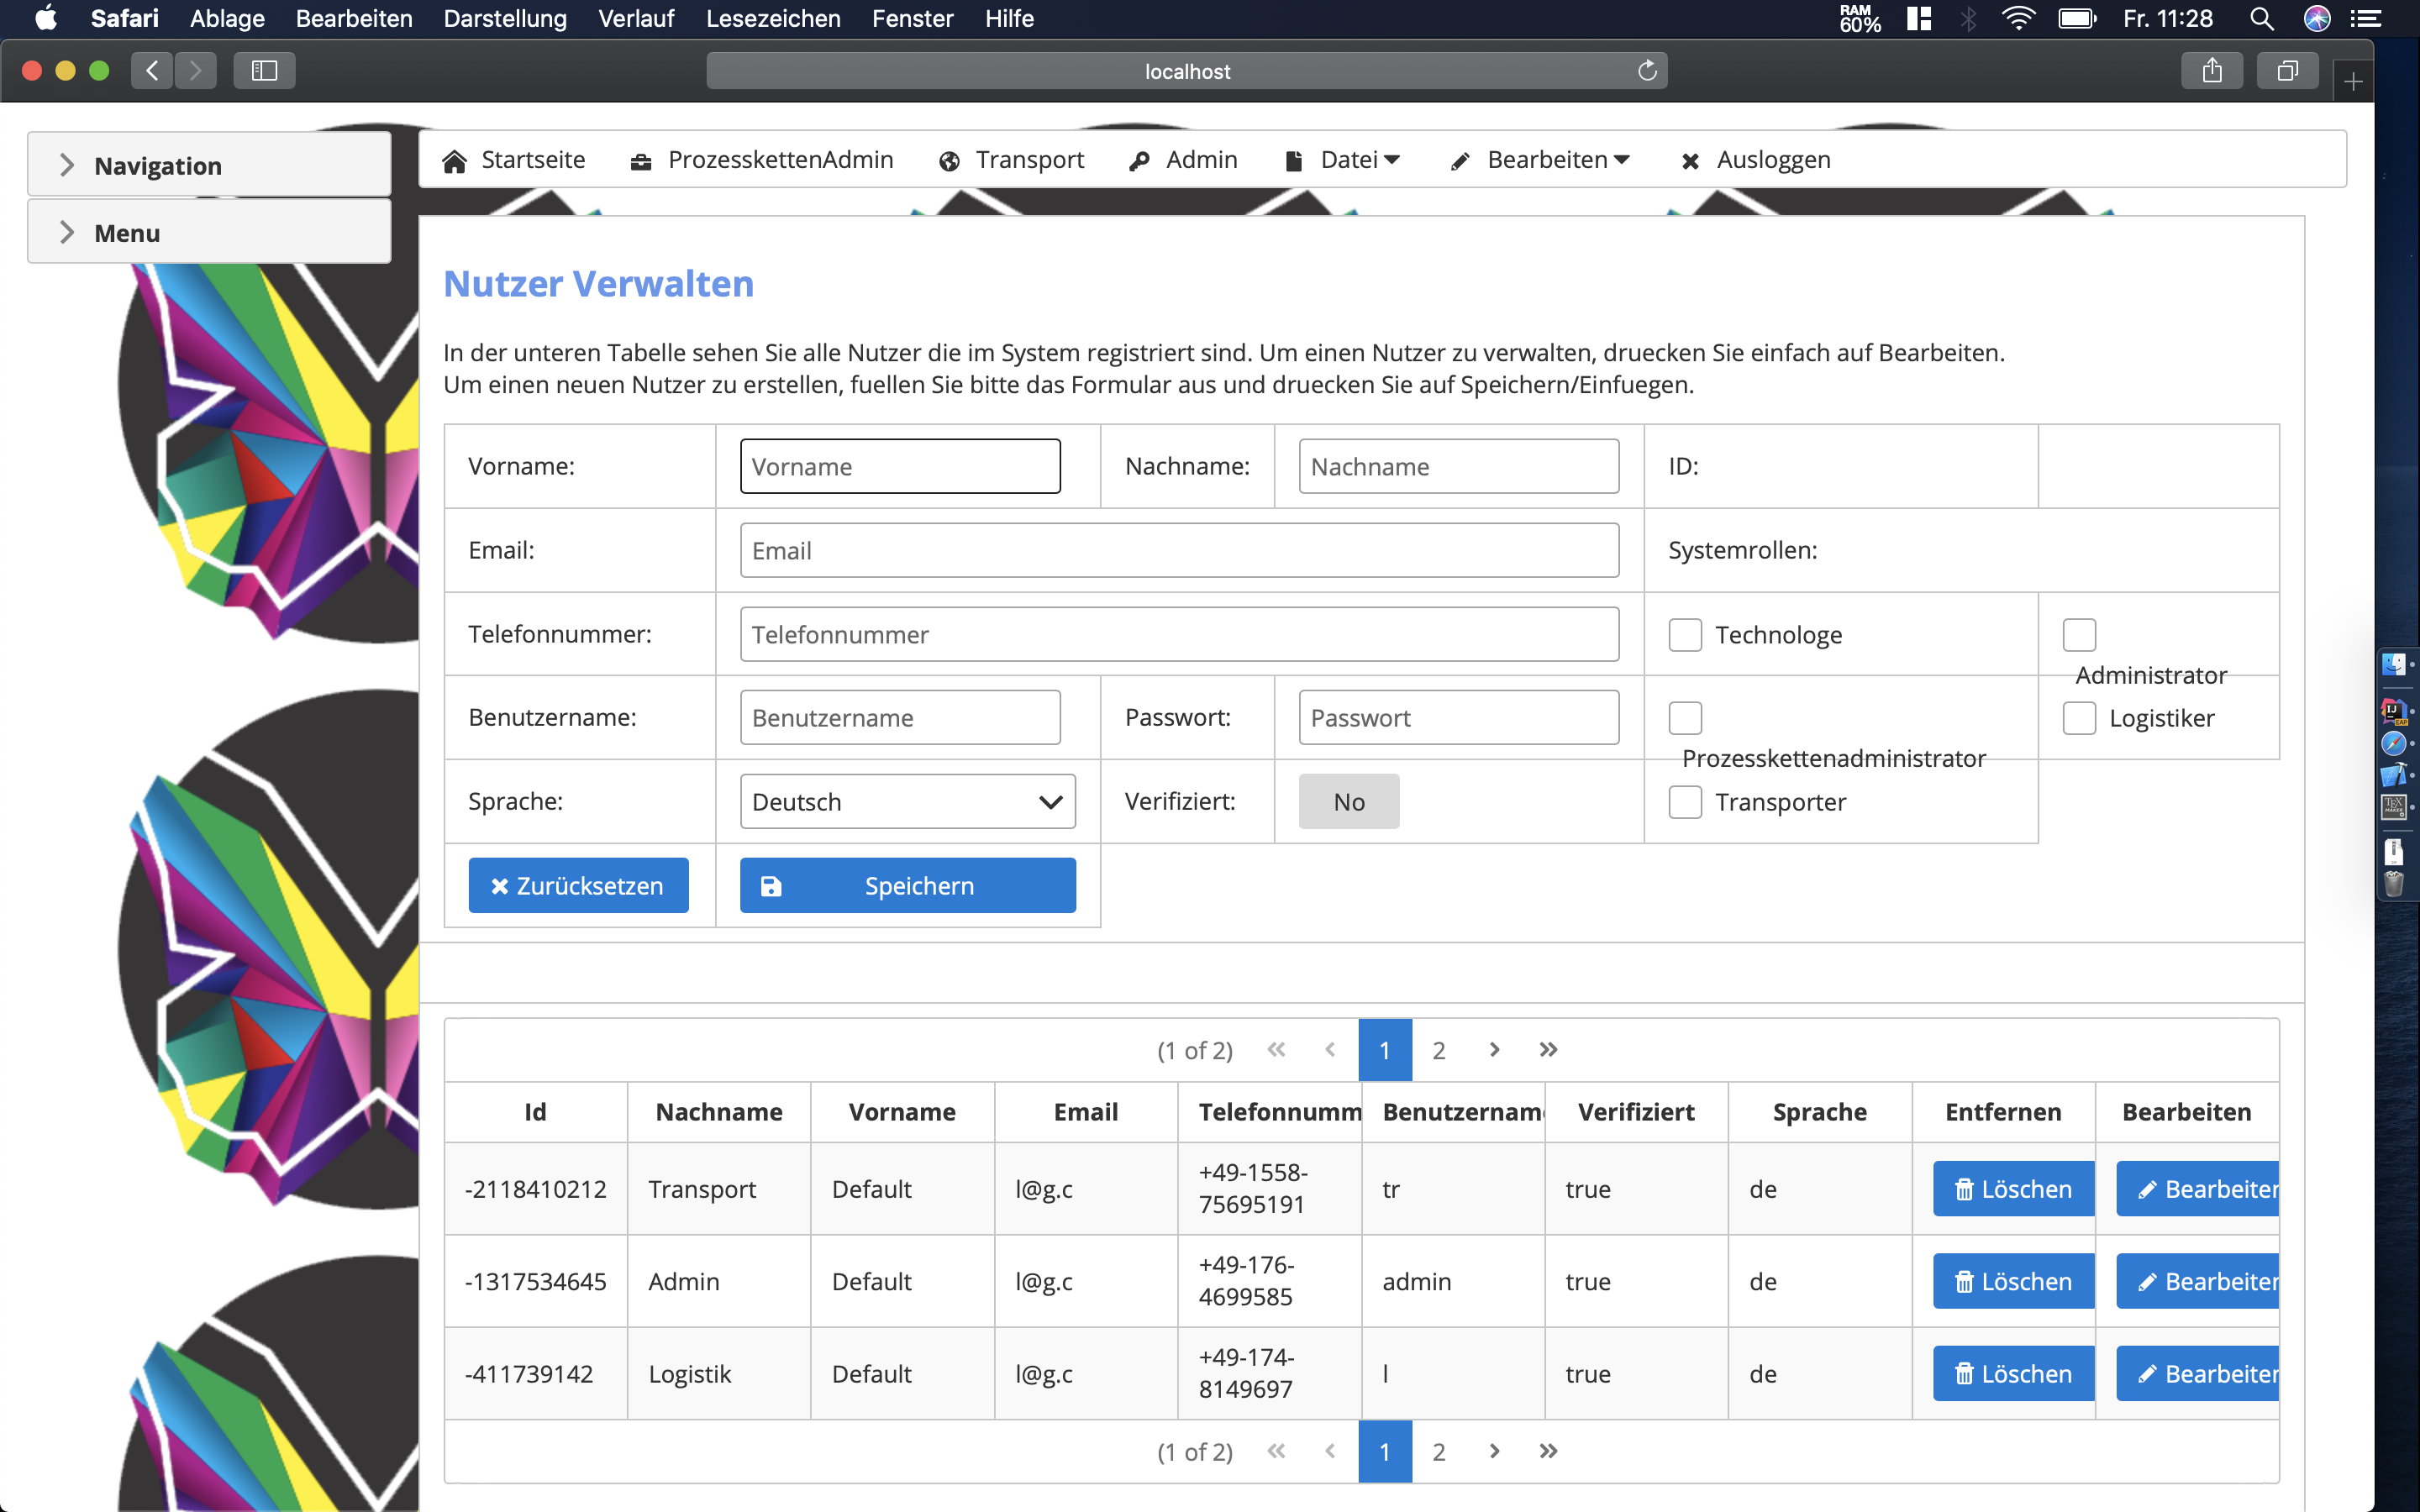
\includegraphics[width=1\textwidth]{Screenshots/UserErzeugenFormular.png}
\textit{Abbildung 3.2.1.1: Benutzer Formular and Tabelle von Benutzer}
} \\

In der folgenden Grafik erstellen wir einen Benutzer mit den entsprechenden Daten.
%%InitialData
\hypertarget{sc3.1.2.2}{
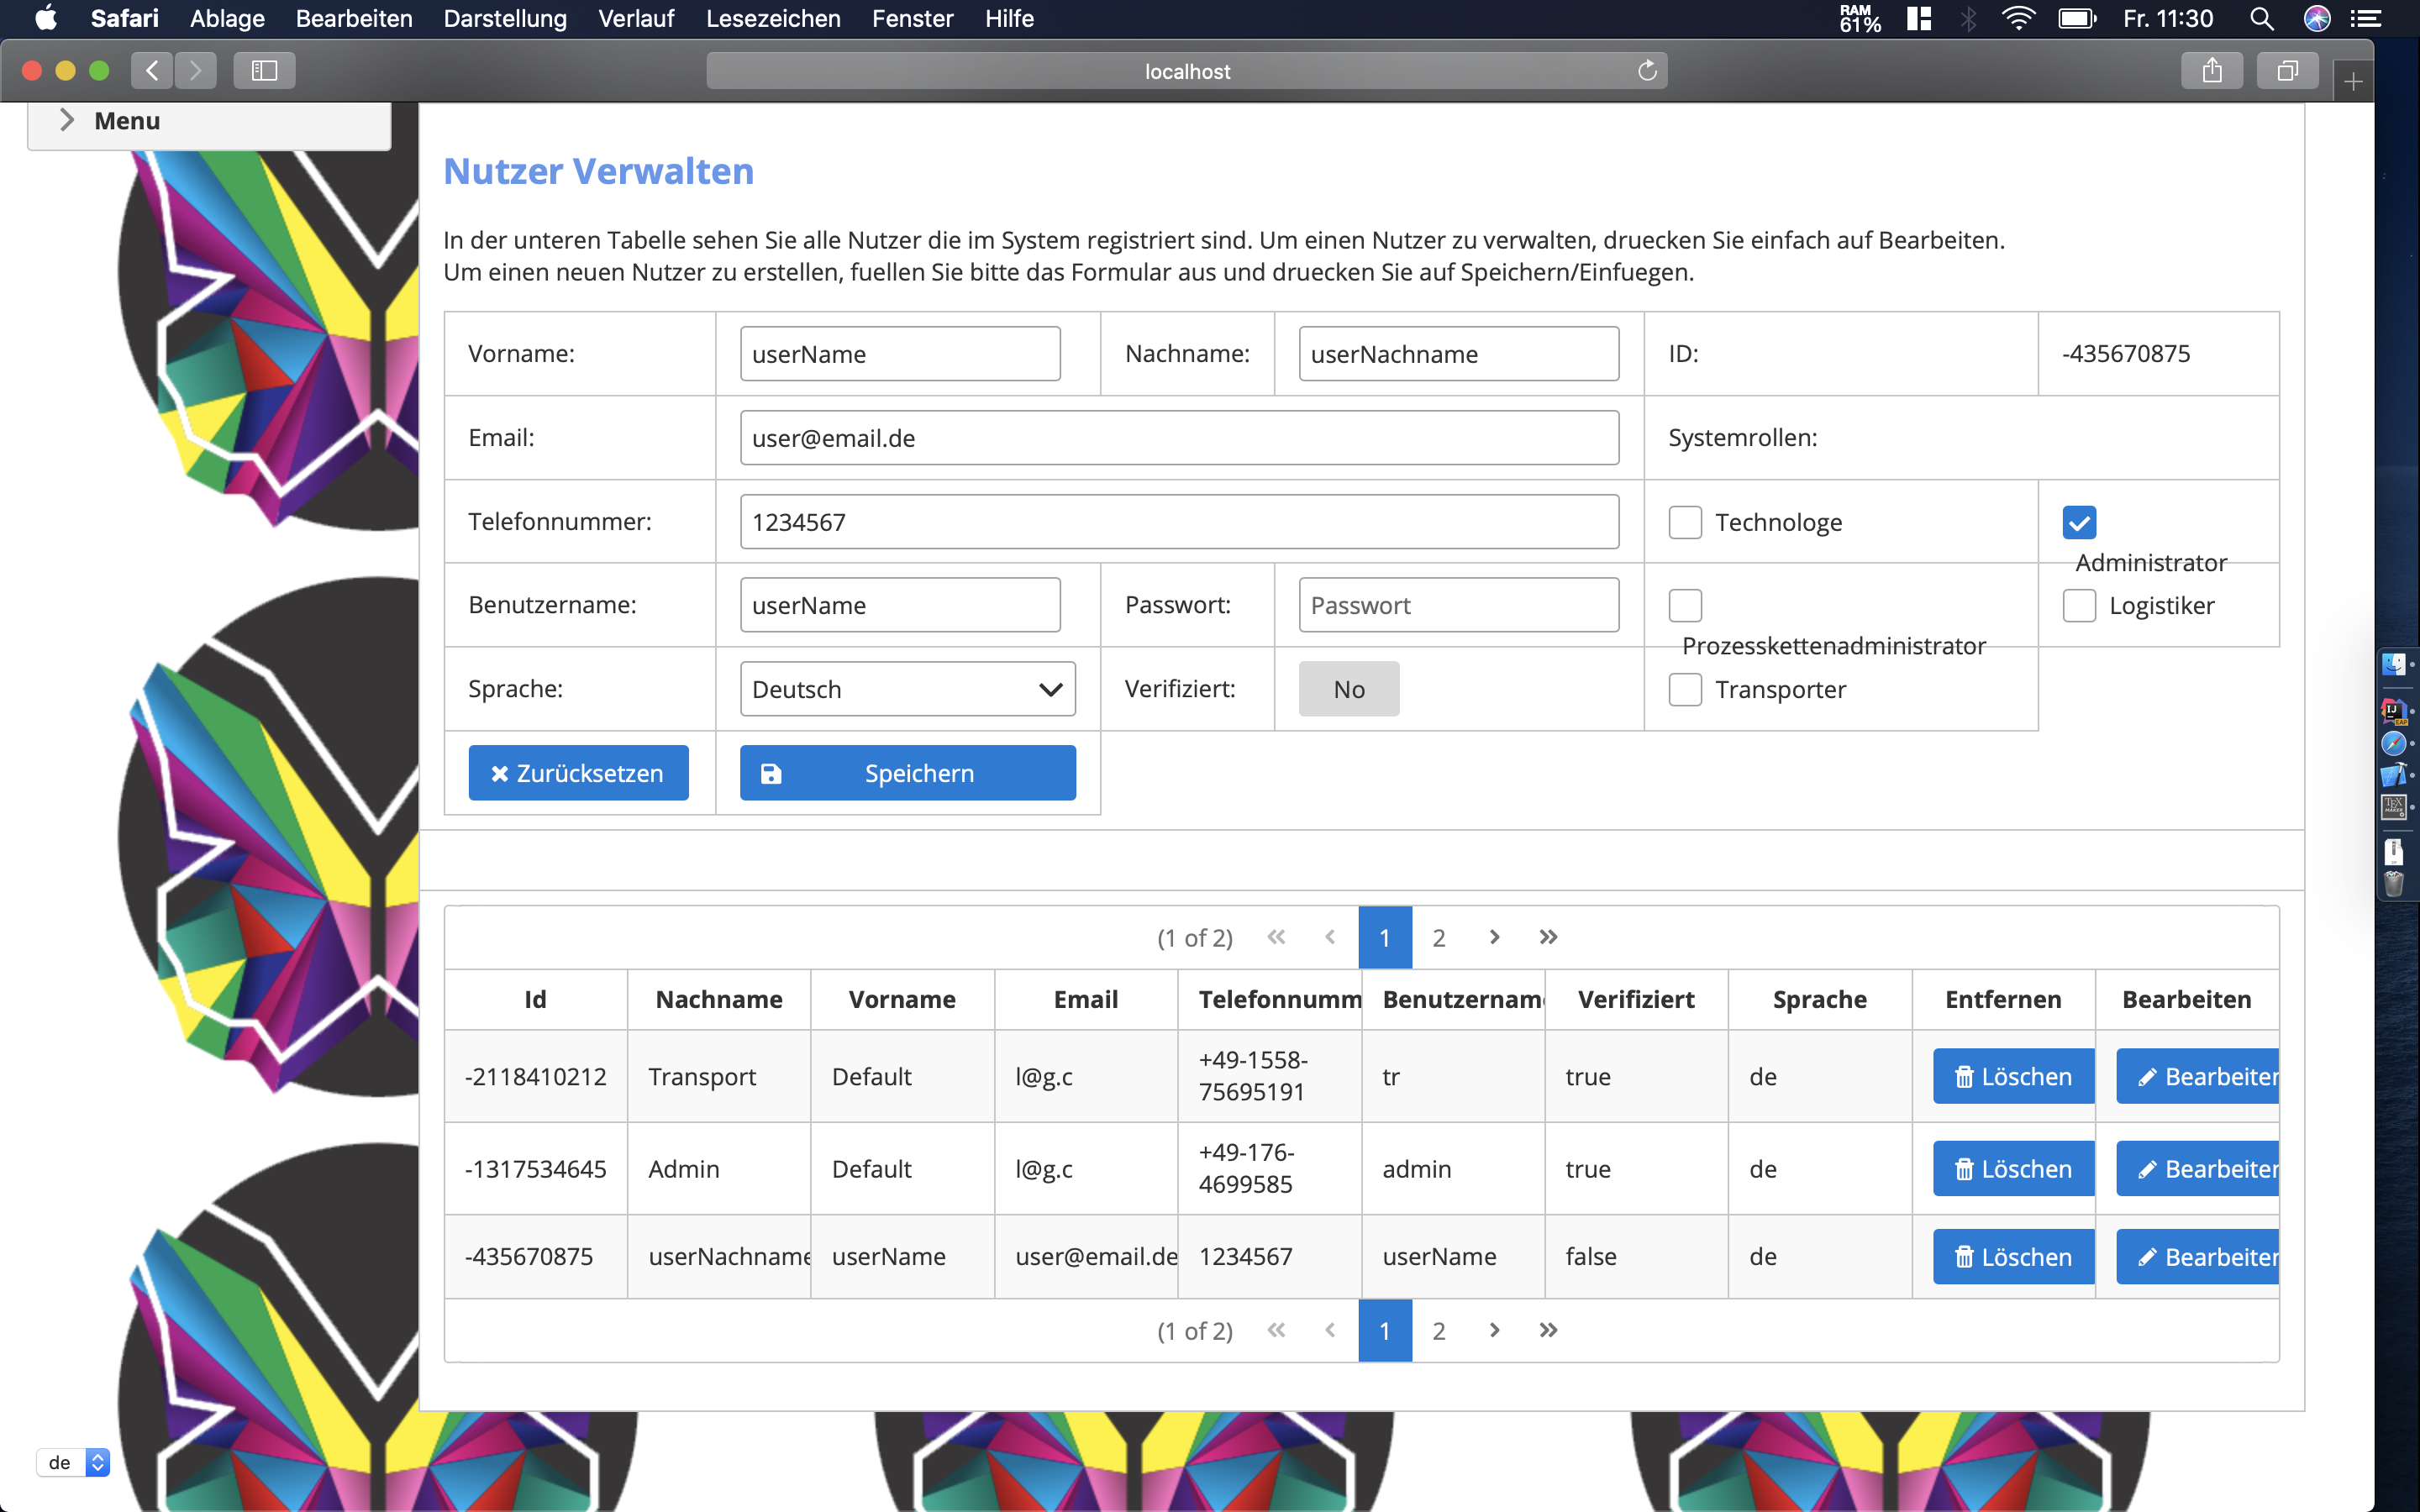
\includegraphics[width=1\textwidth]{Screenshots/userErzeugungInitialData.png}
\textit{Abbildung 3.2.1.2: Pruebe Data für ein neues Benutzer}
} \\
nach dem Drücken der Speichern-Taste. Wir erhalten eine Bestätigung der Software, dass der Benutzer erfolgreich gespeichert wurde.
%%ErzeugunMeldung
\hypertarget{sc3.1.2.3}{
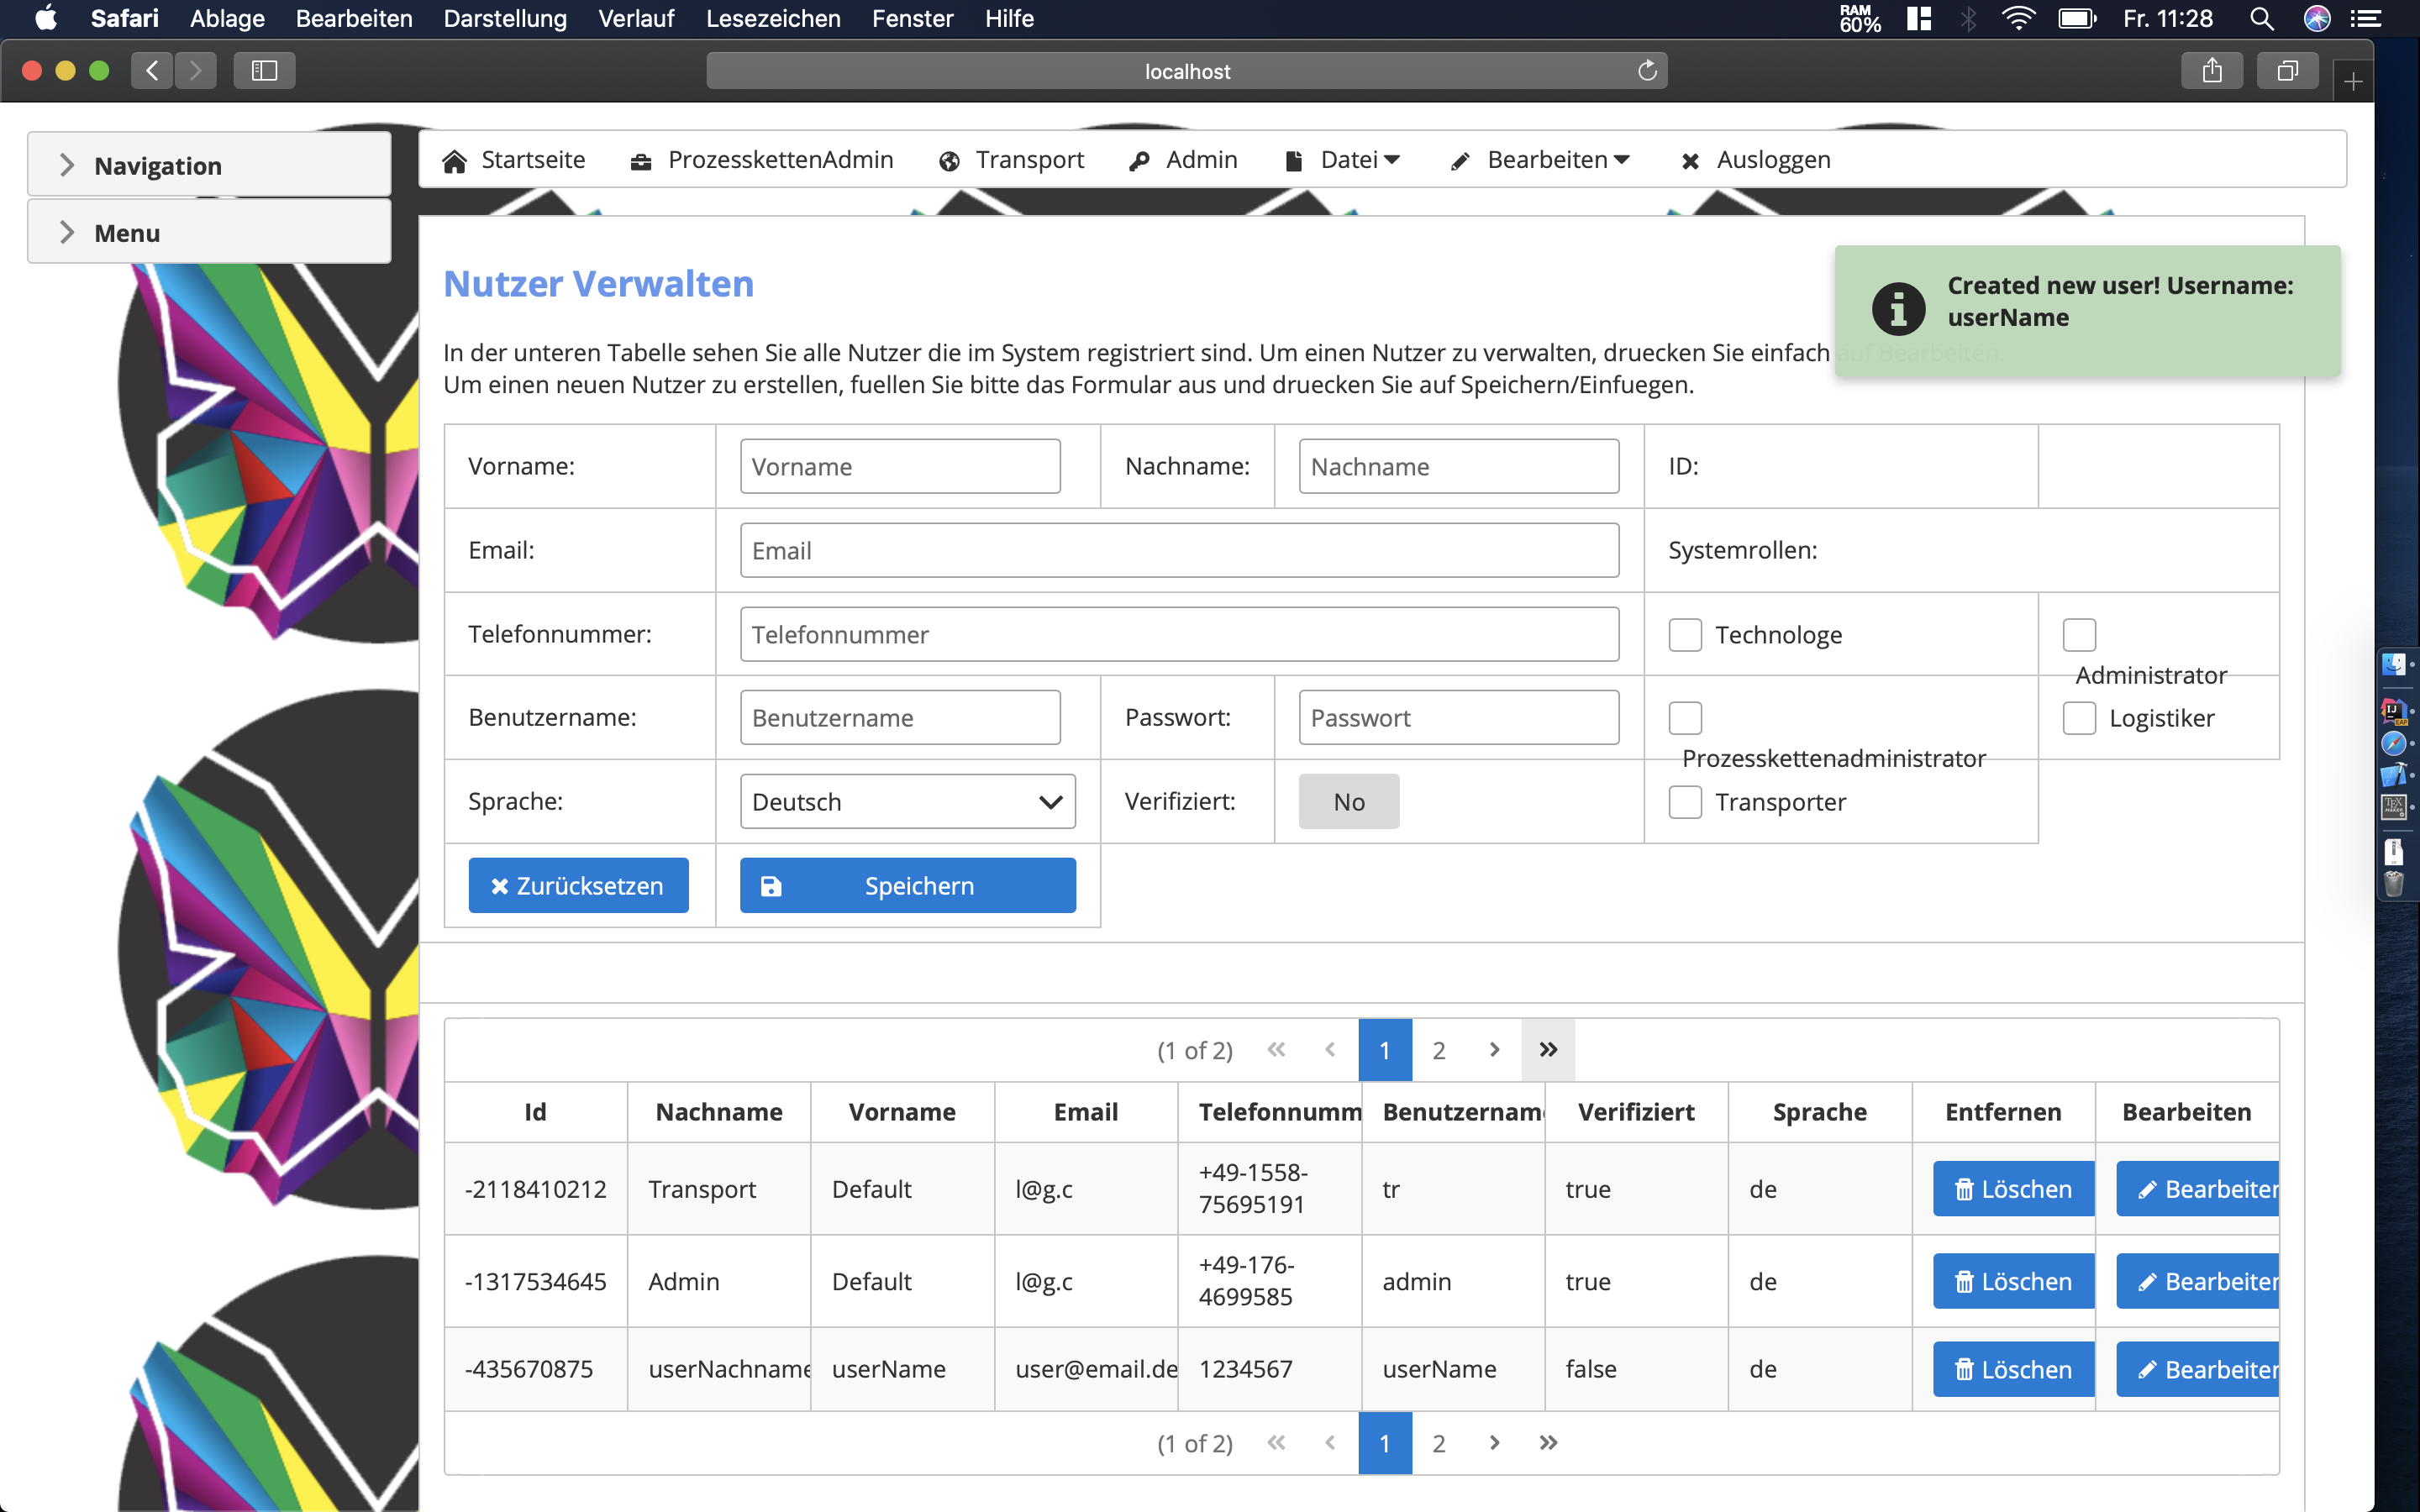
\includegraphics[width=1\textwidth]{Screenshots/userErzeugenMeldung.png}
\textit{Abbildung 3.2.1.3: Meldung von neuer Benutzer an der Webseite}
} \\

Um die spezifischen Informationen zuvor gespeicherter Benutzer zu bearbeiten, drücken Sie die Taste Bwerden. Bearbeiten Sie anschließend die Daten im Formular und klicken Sie abschließend auf die Schaltfläche Speichern.
%%Bearbeiten
\hypertarget{sc3.1.2.4}{
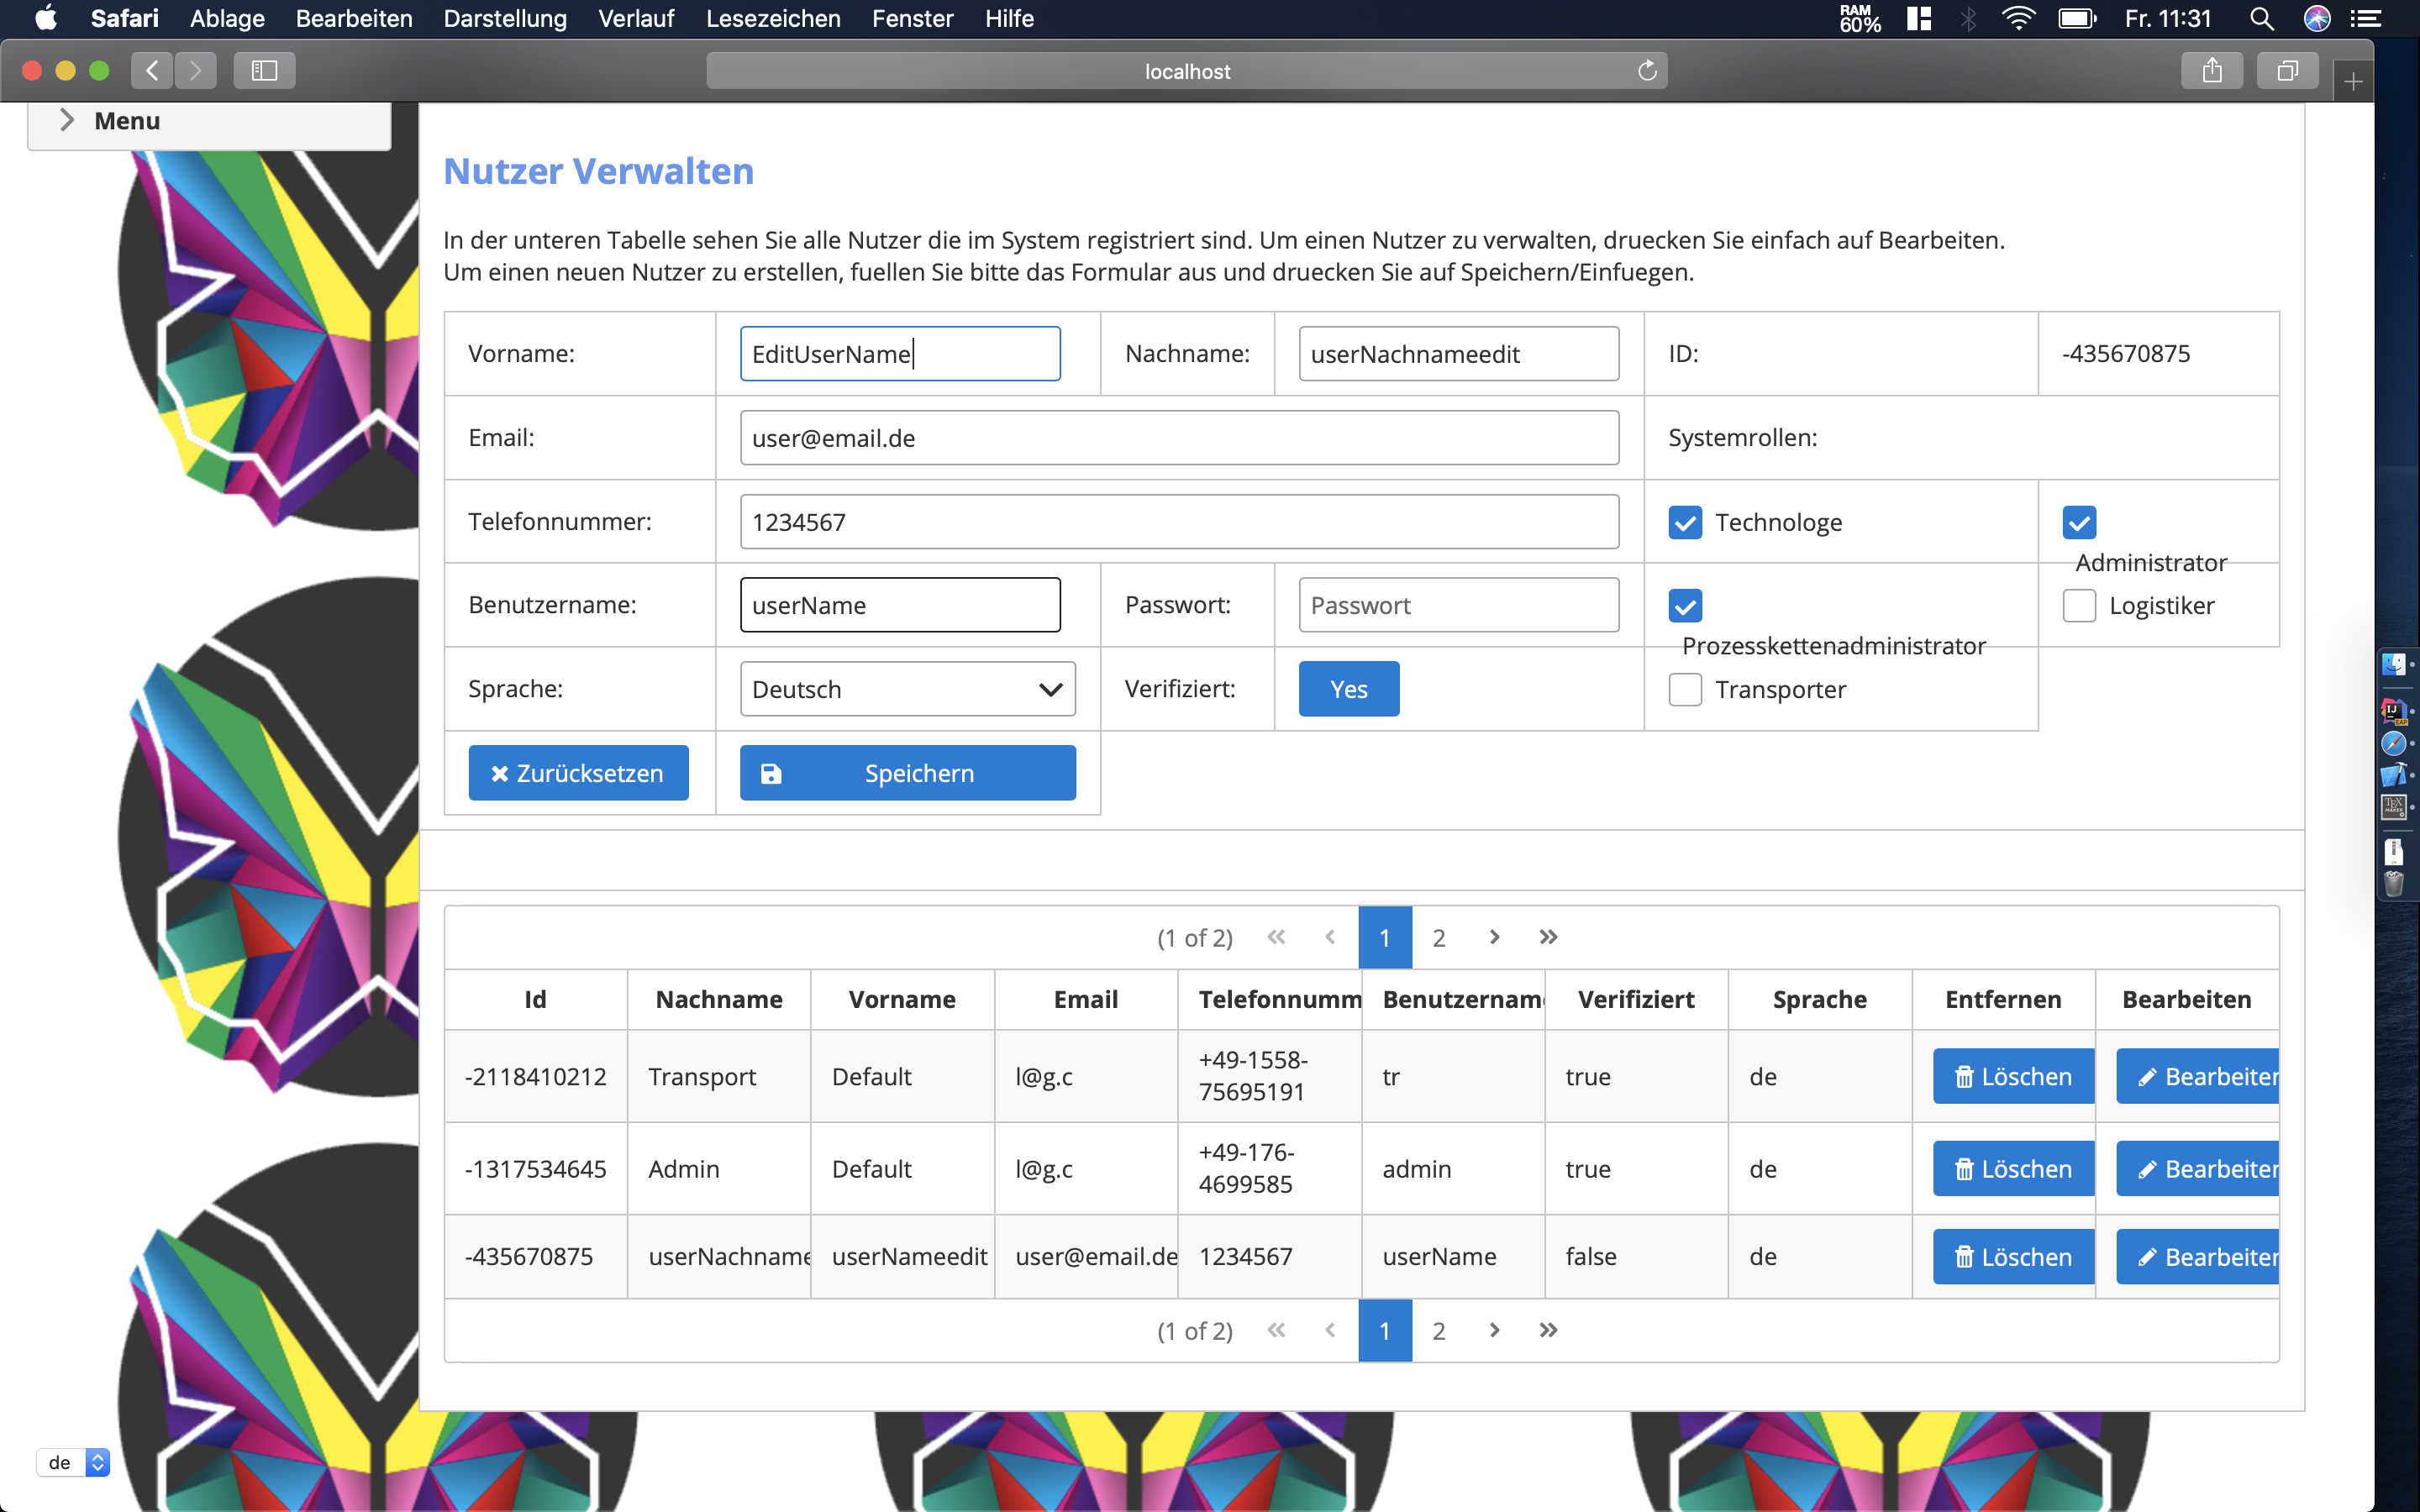
\includegraphics[width=1\textwidth]{Screenshots/UserEditData.png}
\textit{Abbildung 3.2.1.4: Bearbeitung von Data an der Pruebe Benutzer}
} \\
Nachdem der Benutzer gespeichert wurde, sendet die Website eine Bestätigungsnachricht. Wenn inkonsistente Daten eingegeben werden, sendet die Website eine Misserfolgsnachricht.
%%Editmeldung
\hypertarget{sc3.1.2.5}{
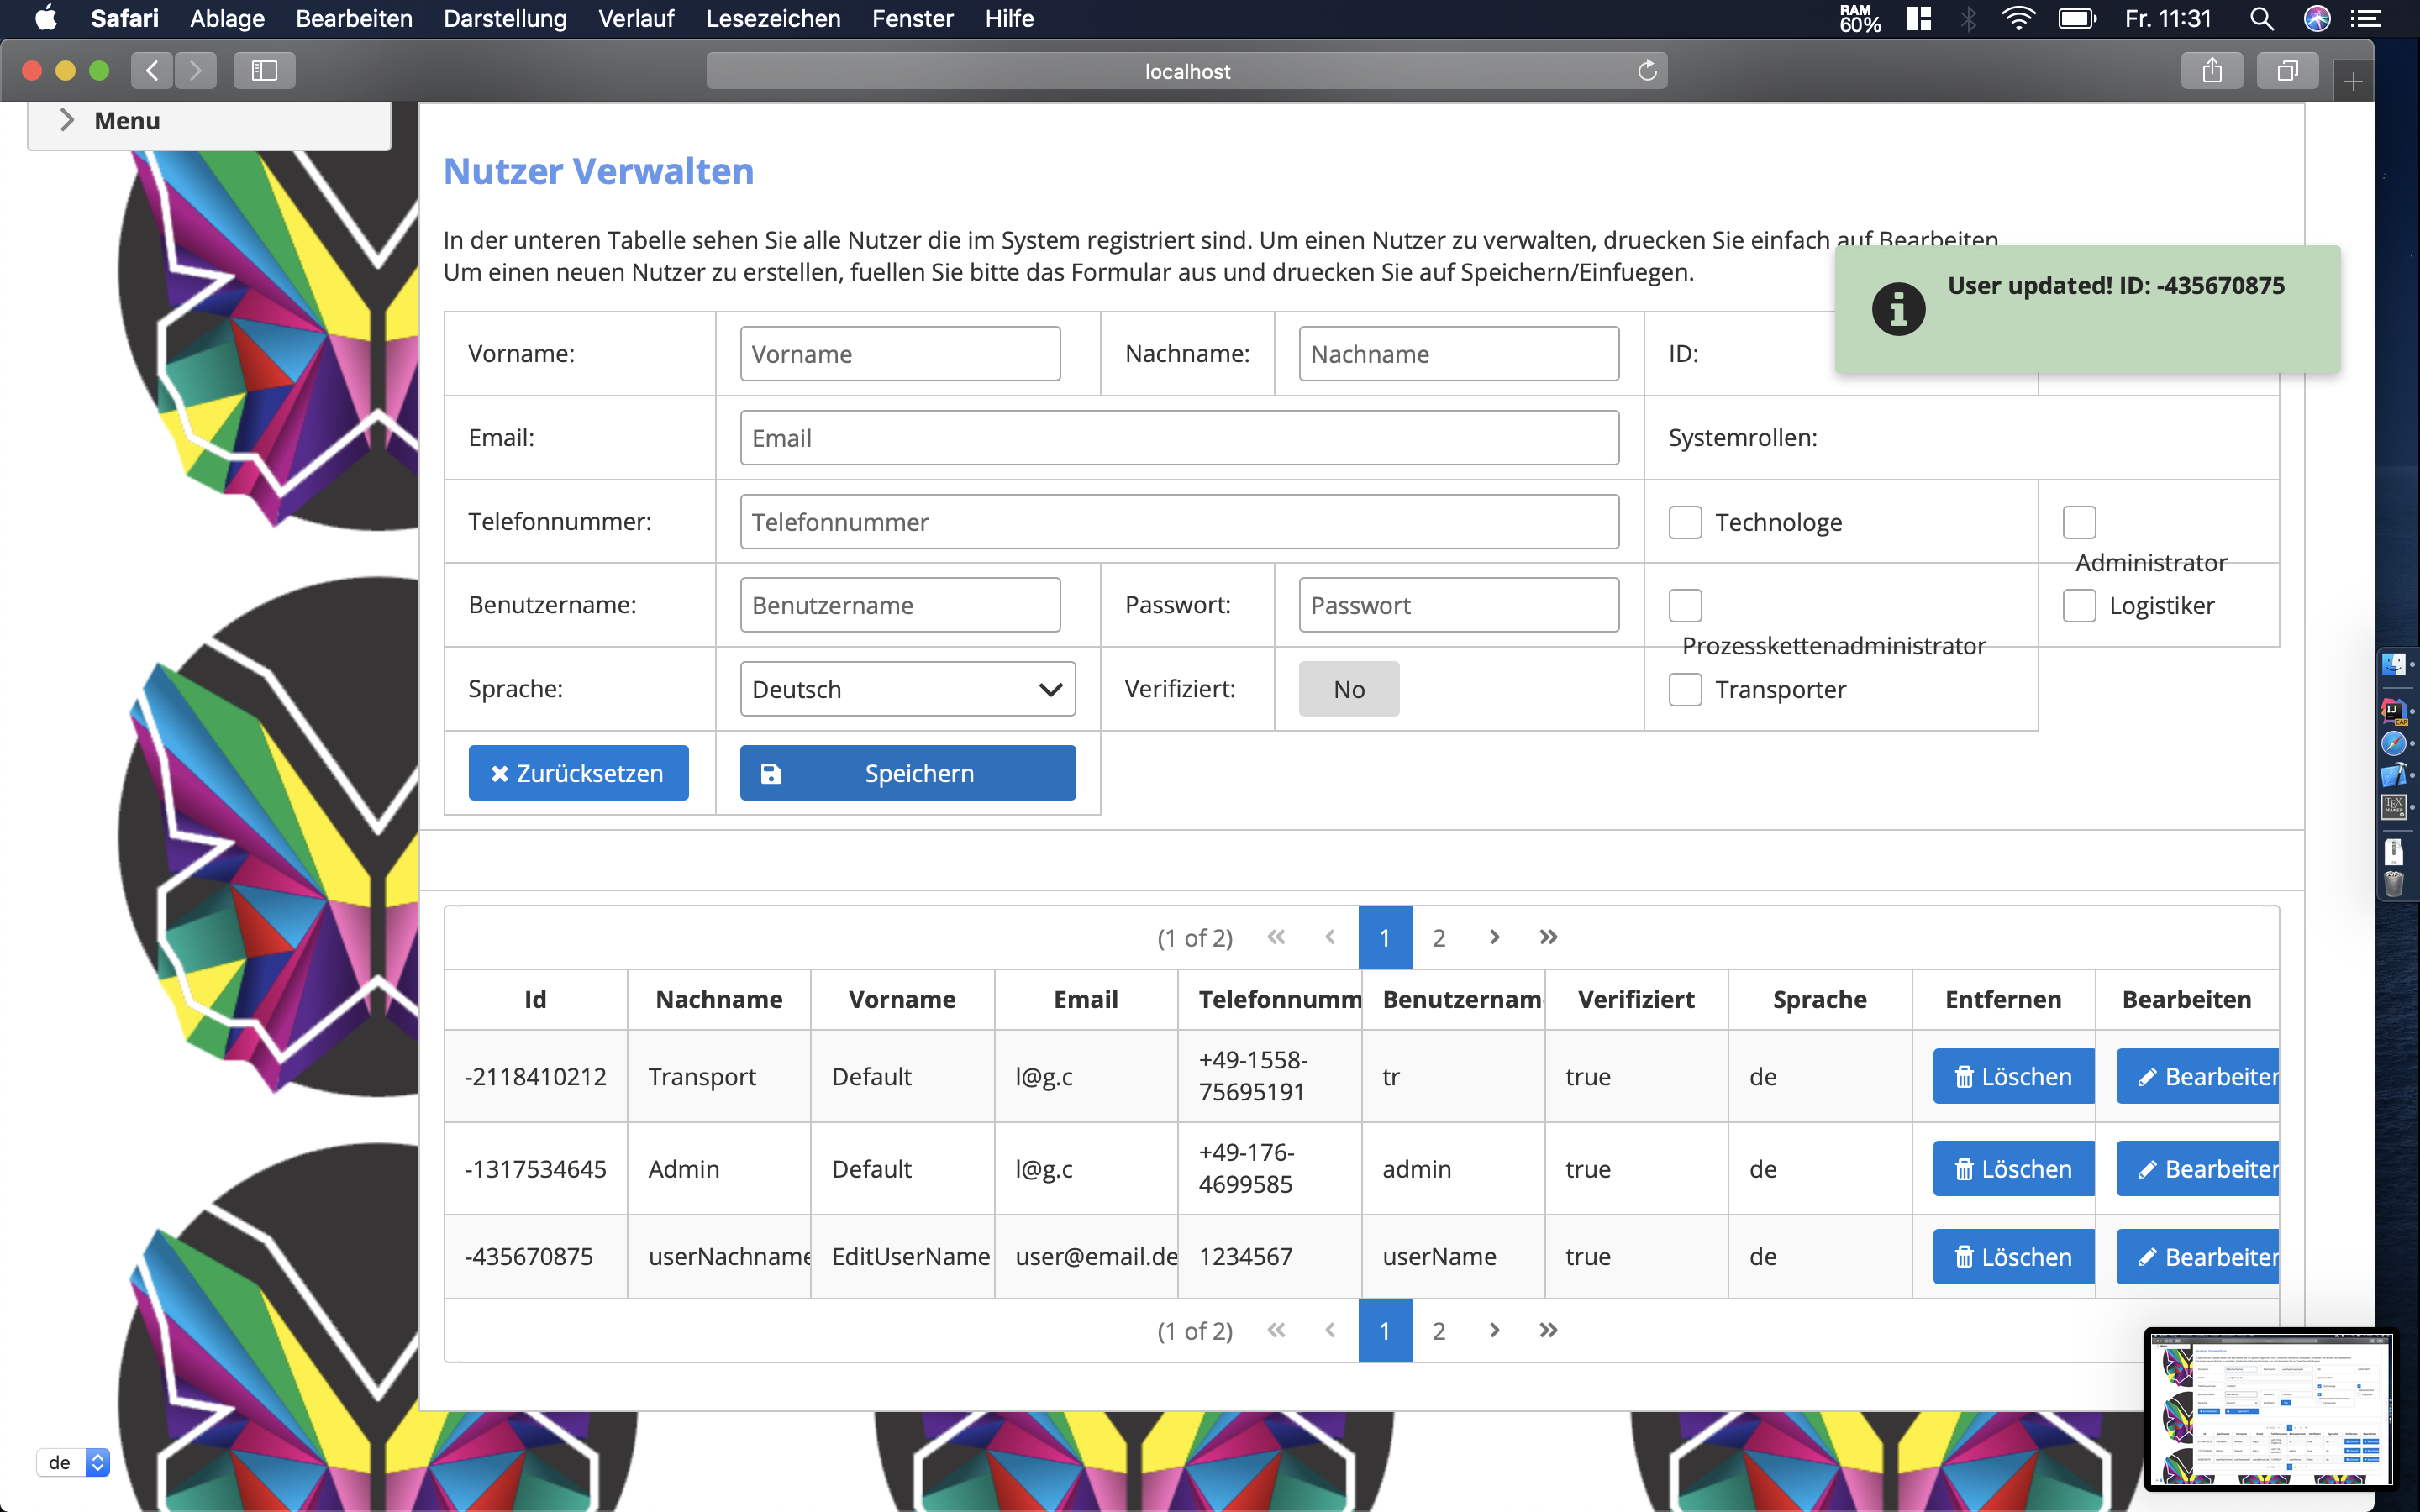
\includegraphics[width=1\textwidth]{Screenshots/editMeldung.png}
\textit{Abbildung 3.2.1.5: Meldung von Erfolgreiche Bearbeitung der Data von nutzer}
} \\


Nachdem der Benutzer editiert wurde, sendet die Website eine Bestätigungsnachricht.
%%InconsistenceData
\hypertarget{sc3.1.2.6}{
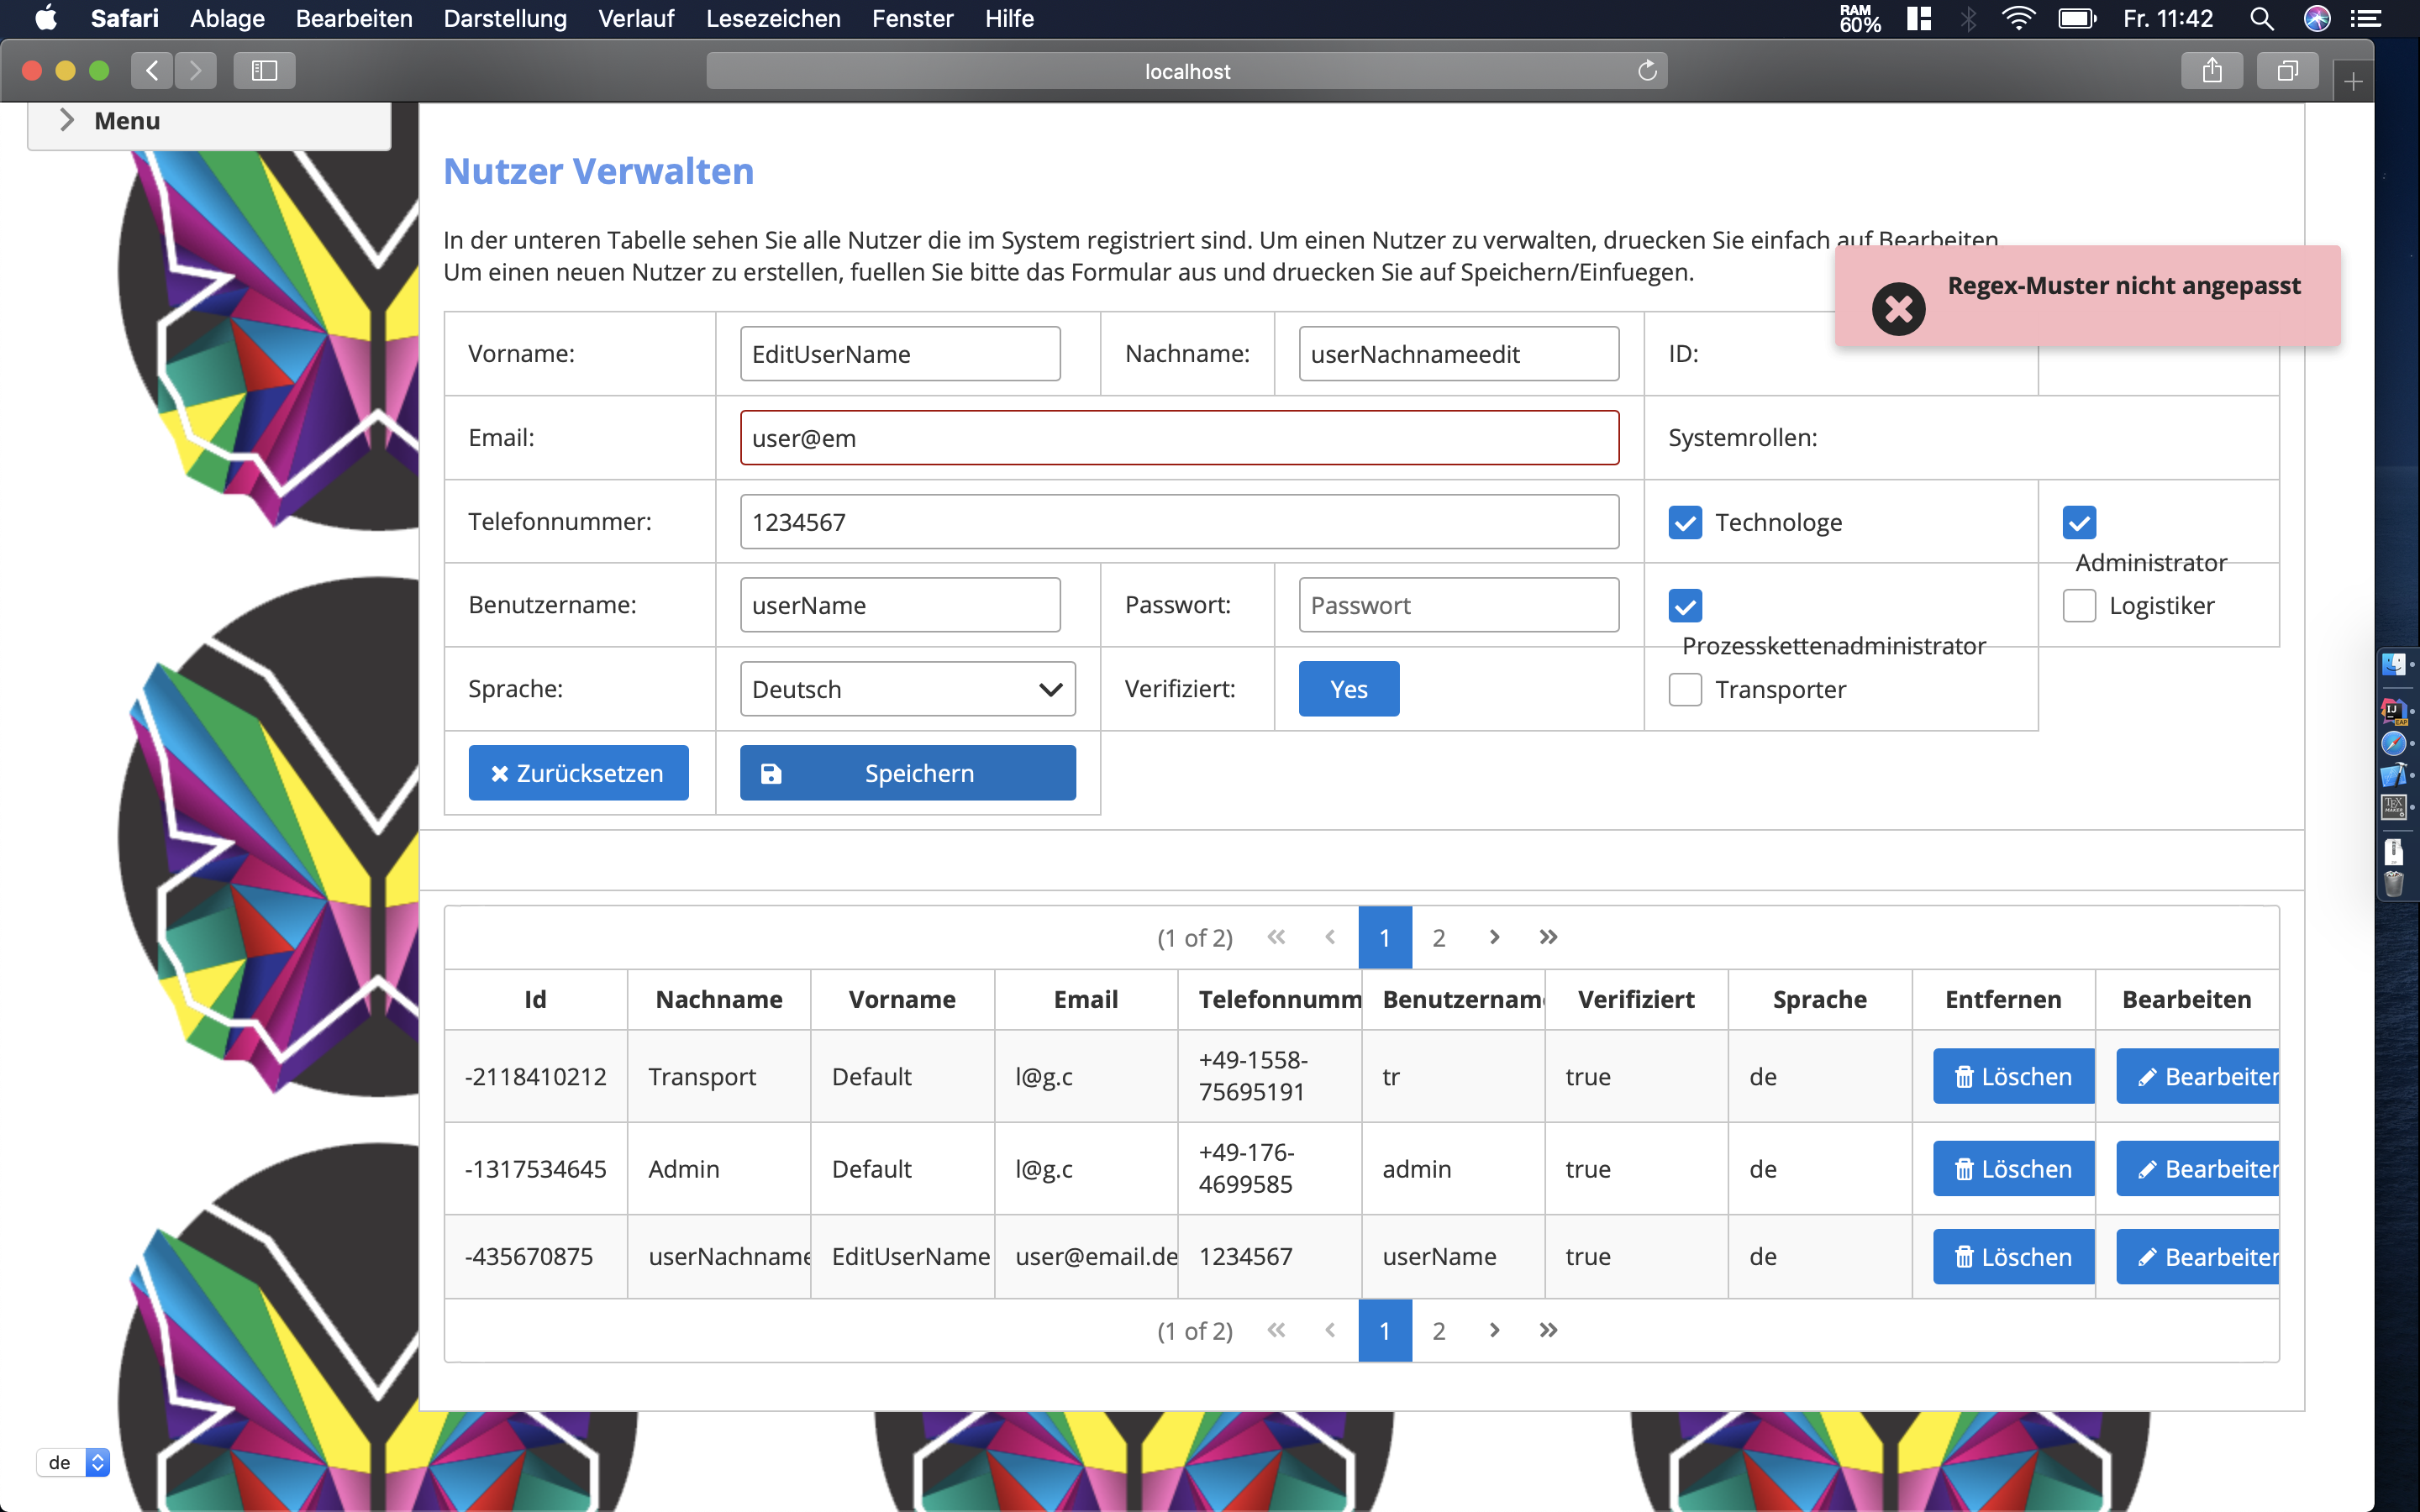
\includegraphics[width=1\textwidth]{Screenshots/InconsistenceDataUserBearbeitung.png}
\textit{Abbildung 3.2.1.6: Meldung von Erfolgreiche Bearbeitung der Data von nutzer}
} \\
Wenn Benutzer gelöscht werden, wird eine Bestätigungsnachricht von der Website abgerufen und der Benutzer wird aus der Benutzertabelle entfernt.
\hypertarget{sc3.1.2.7}{
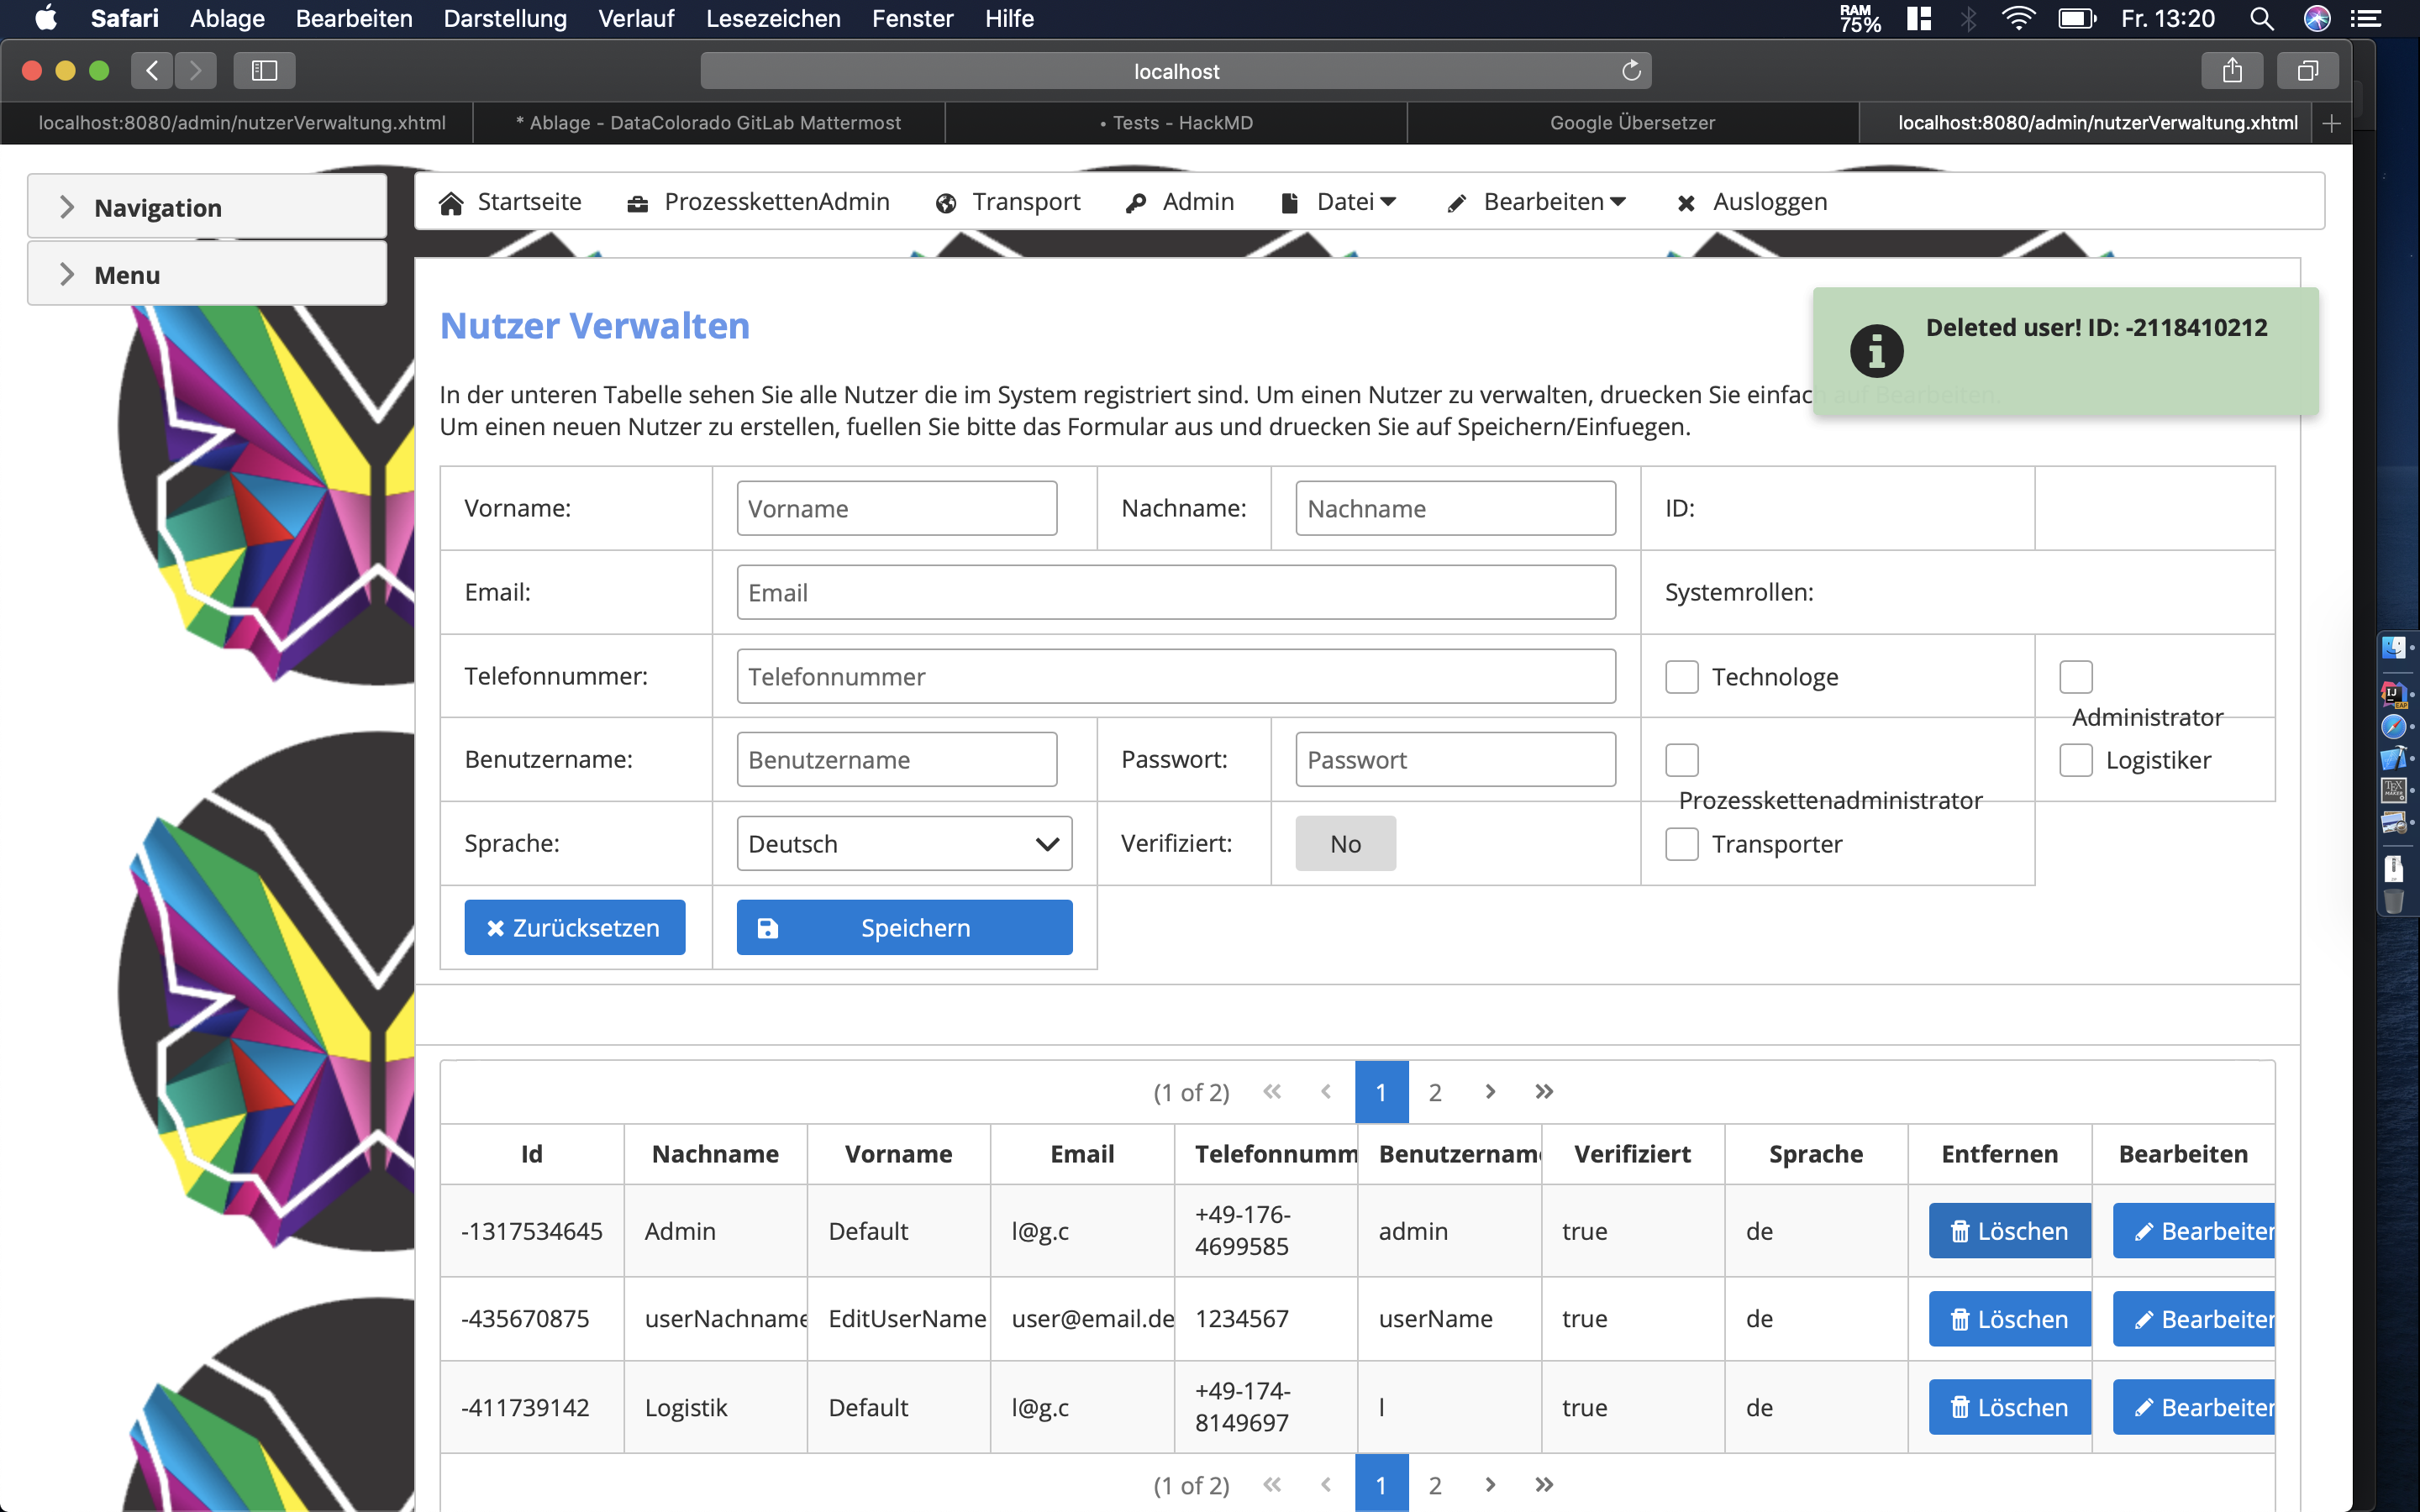
\includegraphics[width=1\textwidth]{Screenshots/BenutzerEntfernen.png}
\textit{Abbildung 3.2.1.7: Meldung von Erfolgreiche Bearbeitung der Data von nutzer}
} \\
%%

\subsubsection{Anwendungsfall: Admin verwaltet Experimentierstation}

Der Admin startet auf seiner \hyperlink{sc3.1.3.1}{Startseite}, nachdem er sich eingeloggt hat. \\

\hypertarget{sc3.1.3.1}{
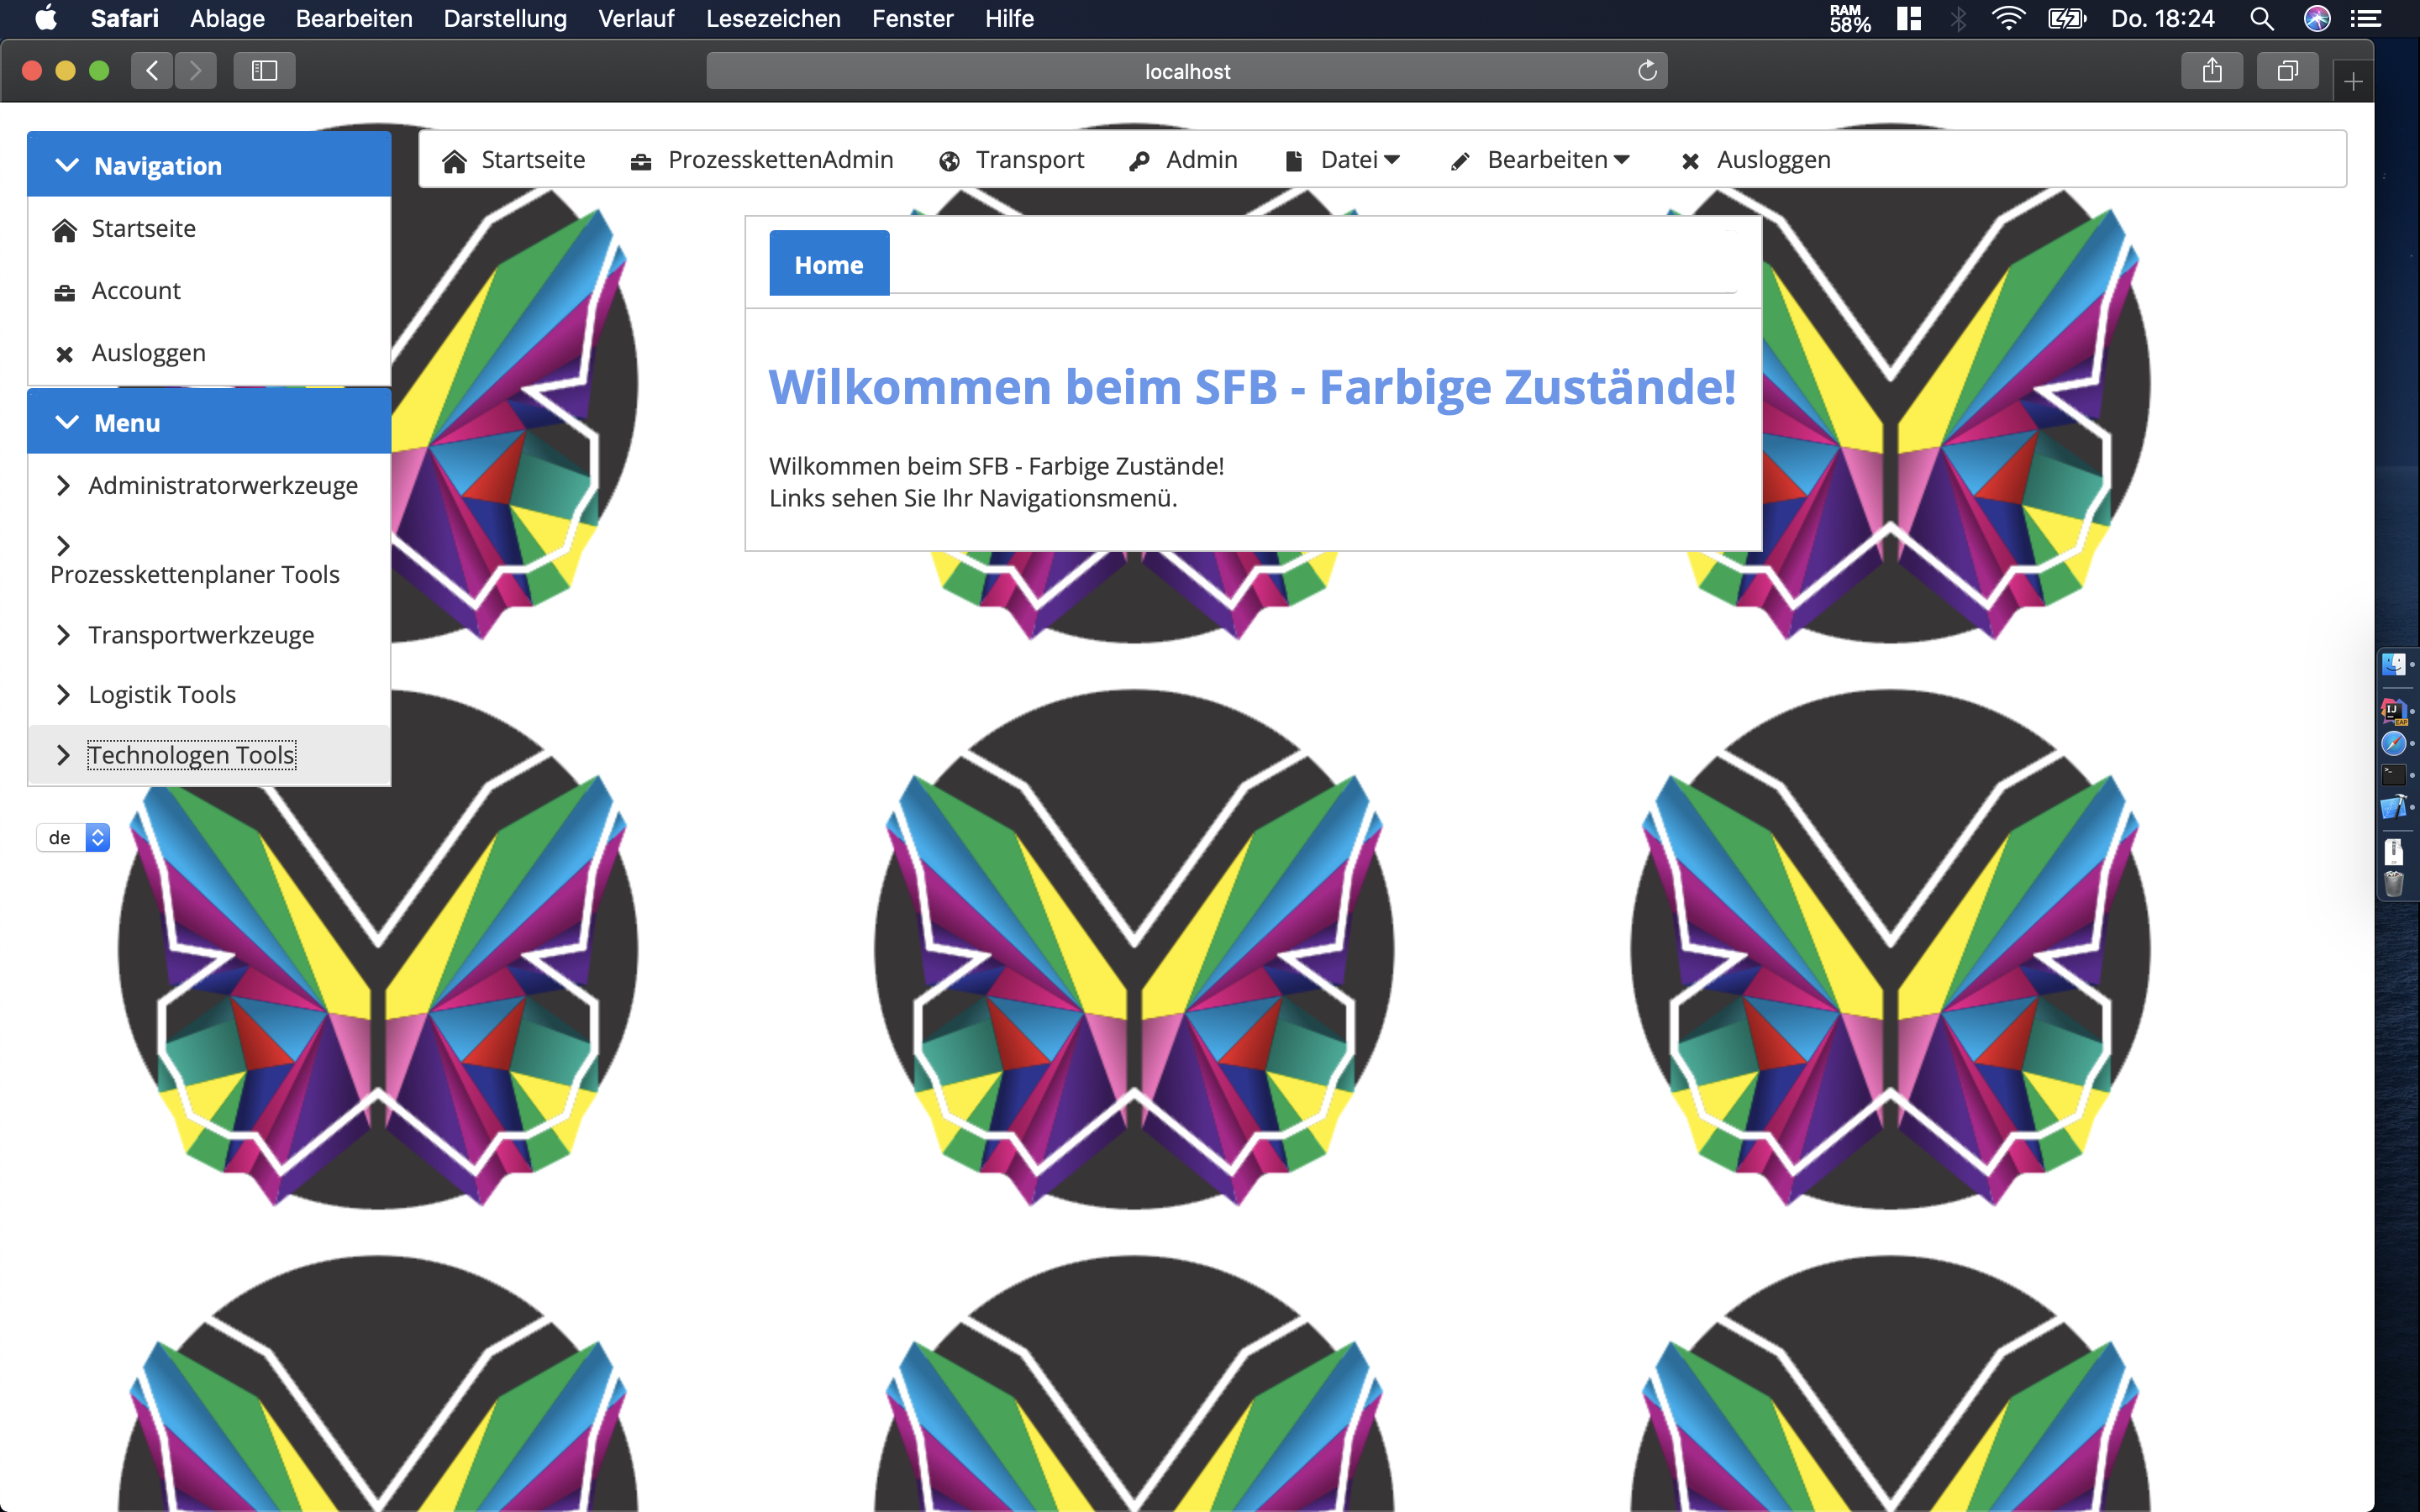
\includegraphics[width=1\textwidth]{Screenshots/311AdminView.png}
\textit{Abbildung 3.2.2.1: Startseite des Admins}
} \\

Er öffnet das Administratorwerkzeuge Menü am linken Bildschirmrand und drückt auf Experimentierstationen verwalten. Nun wird er auf die Seite zum \hyperlink{sc3.1.3.2}{Verwalten der Experimentierstationen} weitergeleitet. \\

\hypertarget{sc3.1.3.2}{
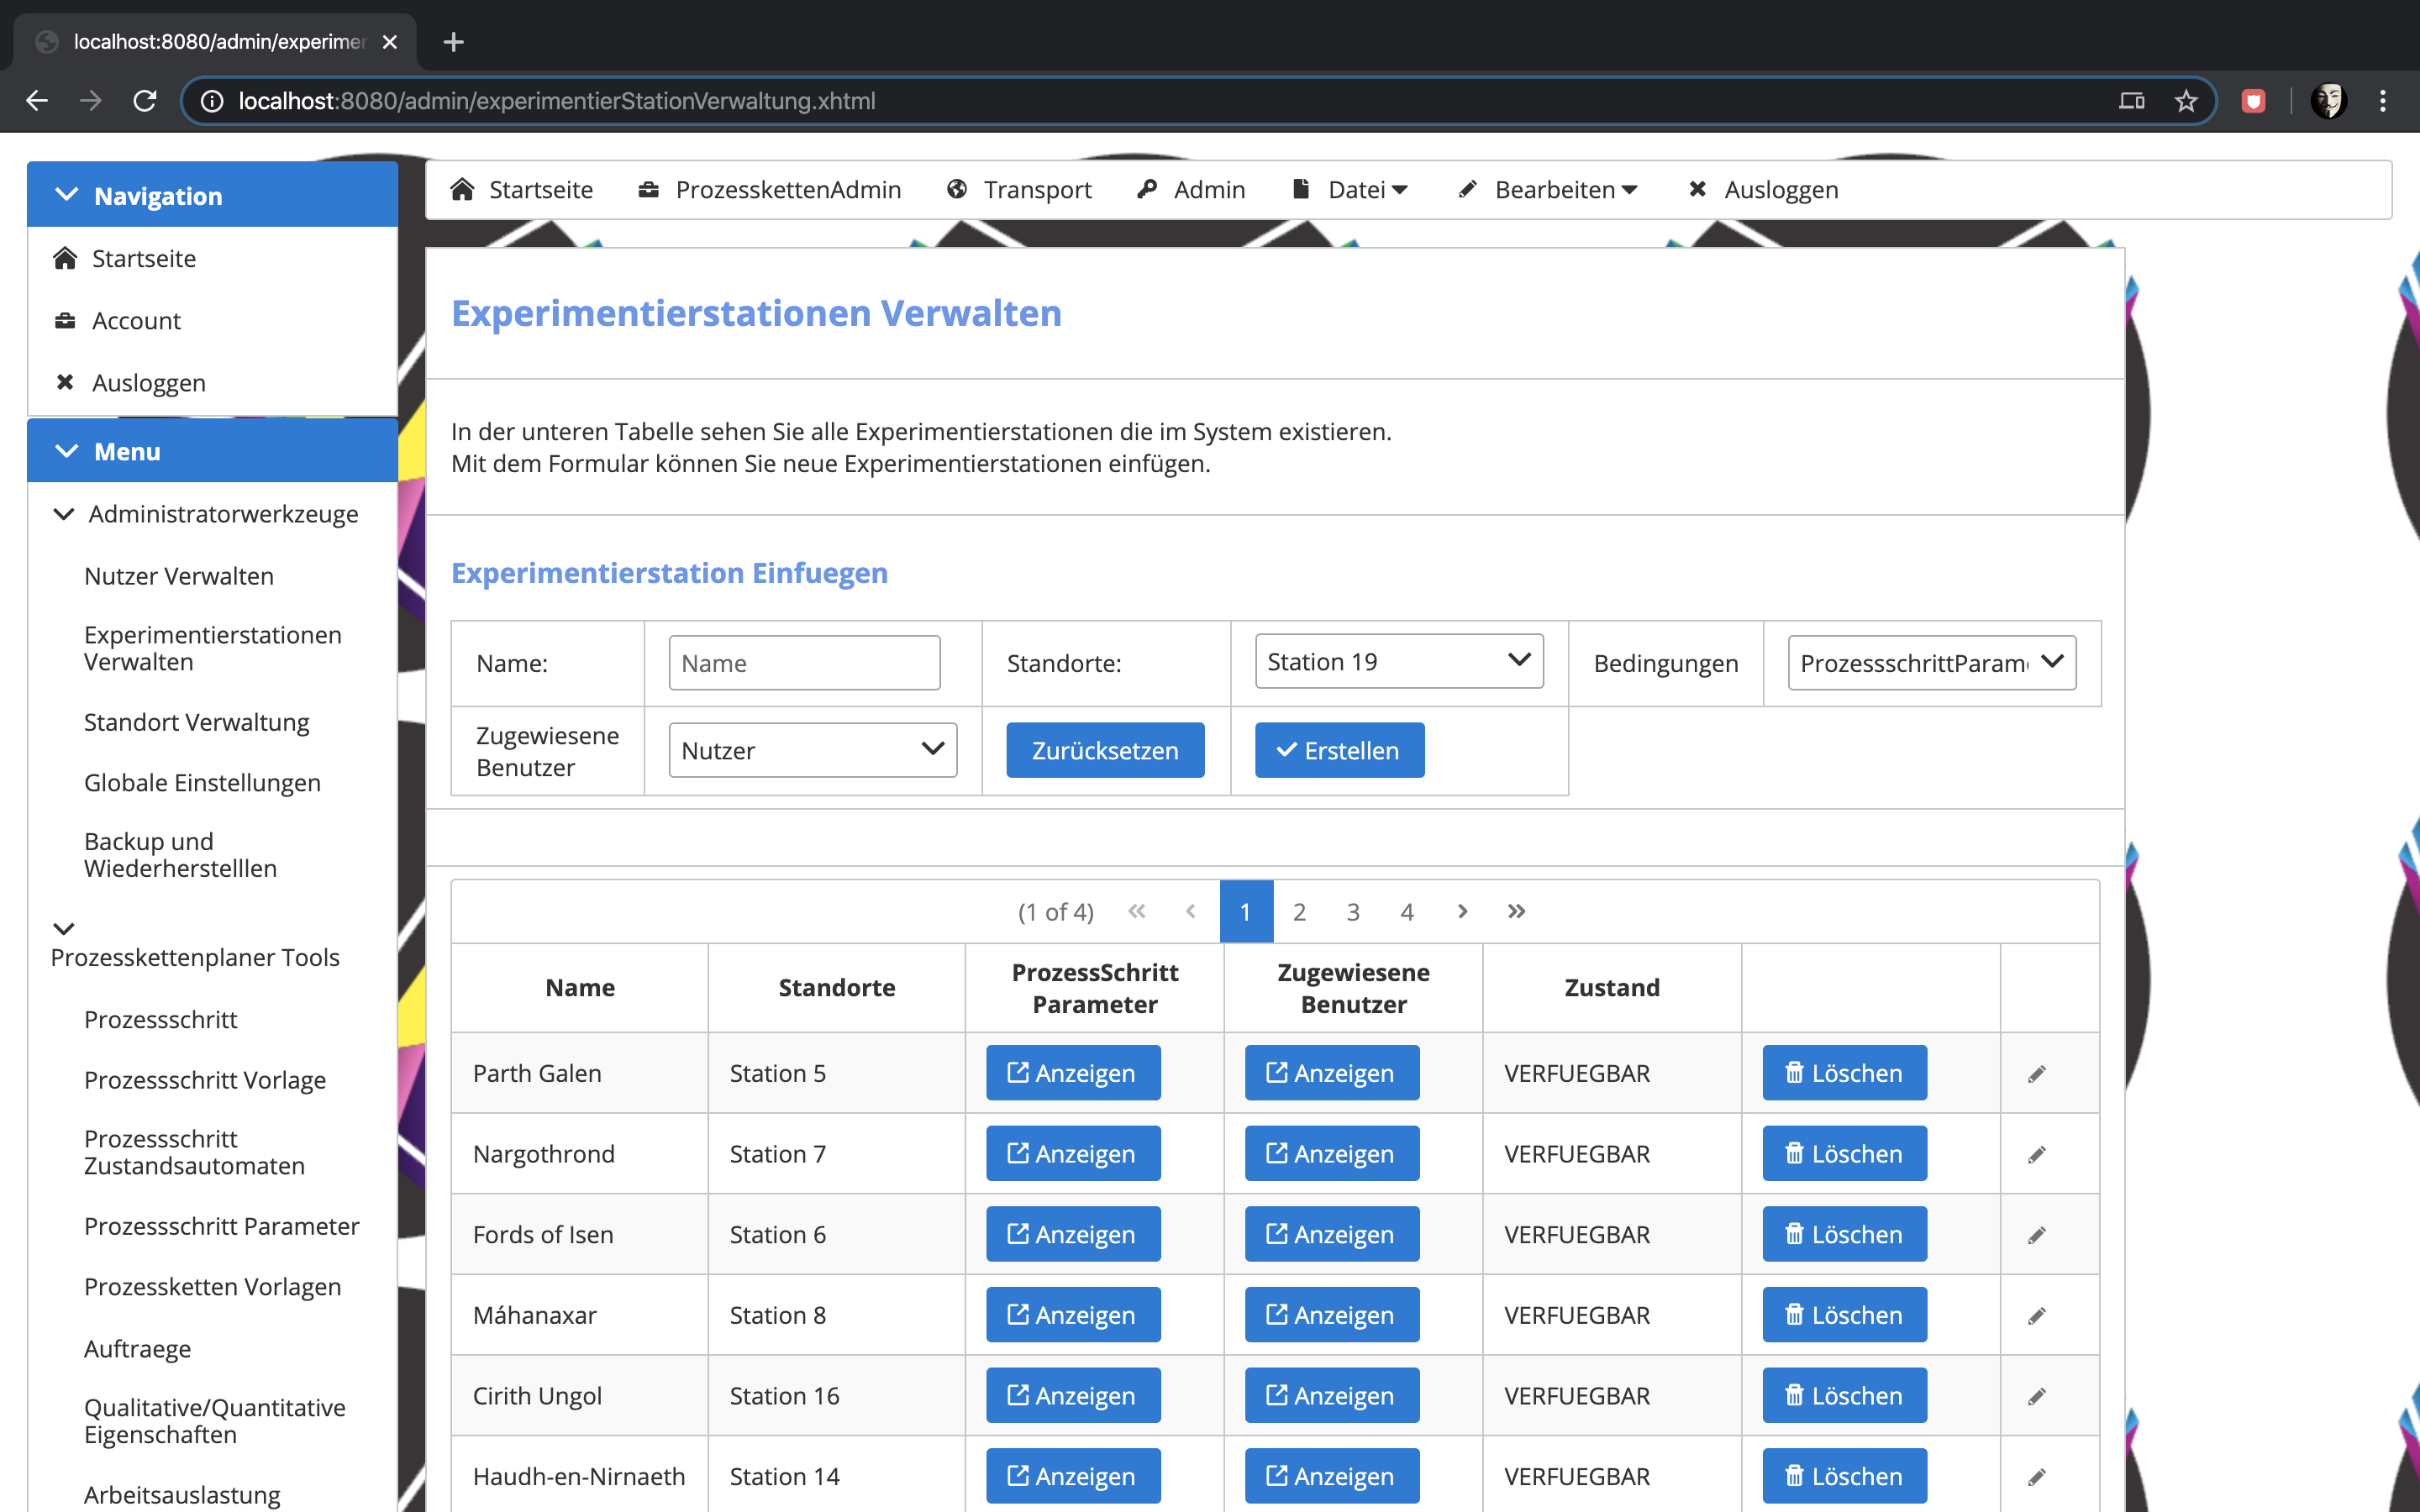
\includegraphics[width=1\textwidth]{Screenshots/3132.png}
\textit{Abbildung 3.2.2.2: Verwalten der Experimentierstationen}
} \\

\paragraph{Erstellen neuer Experimentierstationen:}

Für das Erstellen einer Experimentierstation benötigt man zwingend einen beliebigen Namen zum Eingeben, einen Standort, an dem die Experimentierstation erstellt wird und einen zugewiesenen Benutzer. Optional können Prozesschrittparameter als Bedingungen angegeben werden. \\

Nun befindet sich der Administrator auf der Seite zum \hyperlink{sc3.1.3.2}{Verwalten der Experimentierstationen}. Oben auf der Seite findet man eine \hyperlink{sc3.1.3.3}{Tabelle zum Einfügen von Experimentierstationen}. \\

\hypertarget{sc3.1.3.3}{
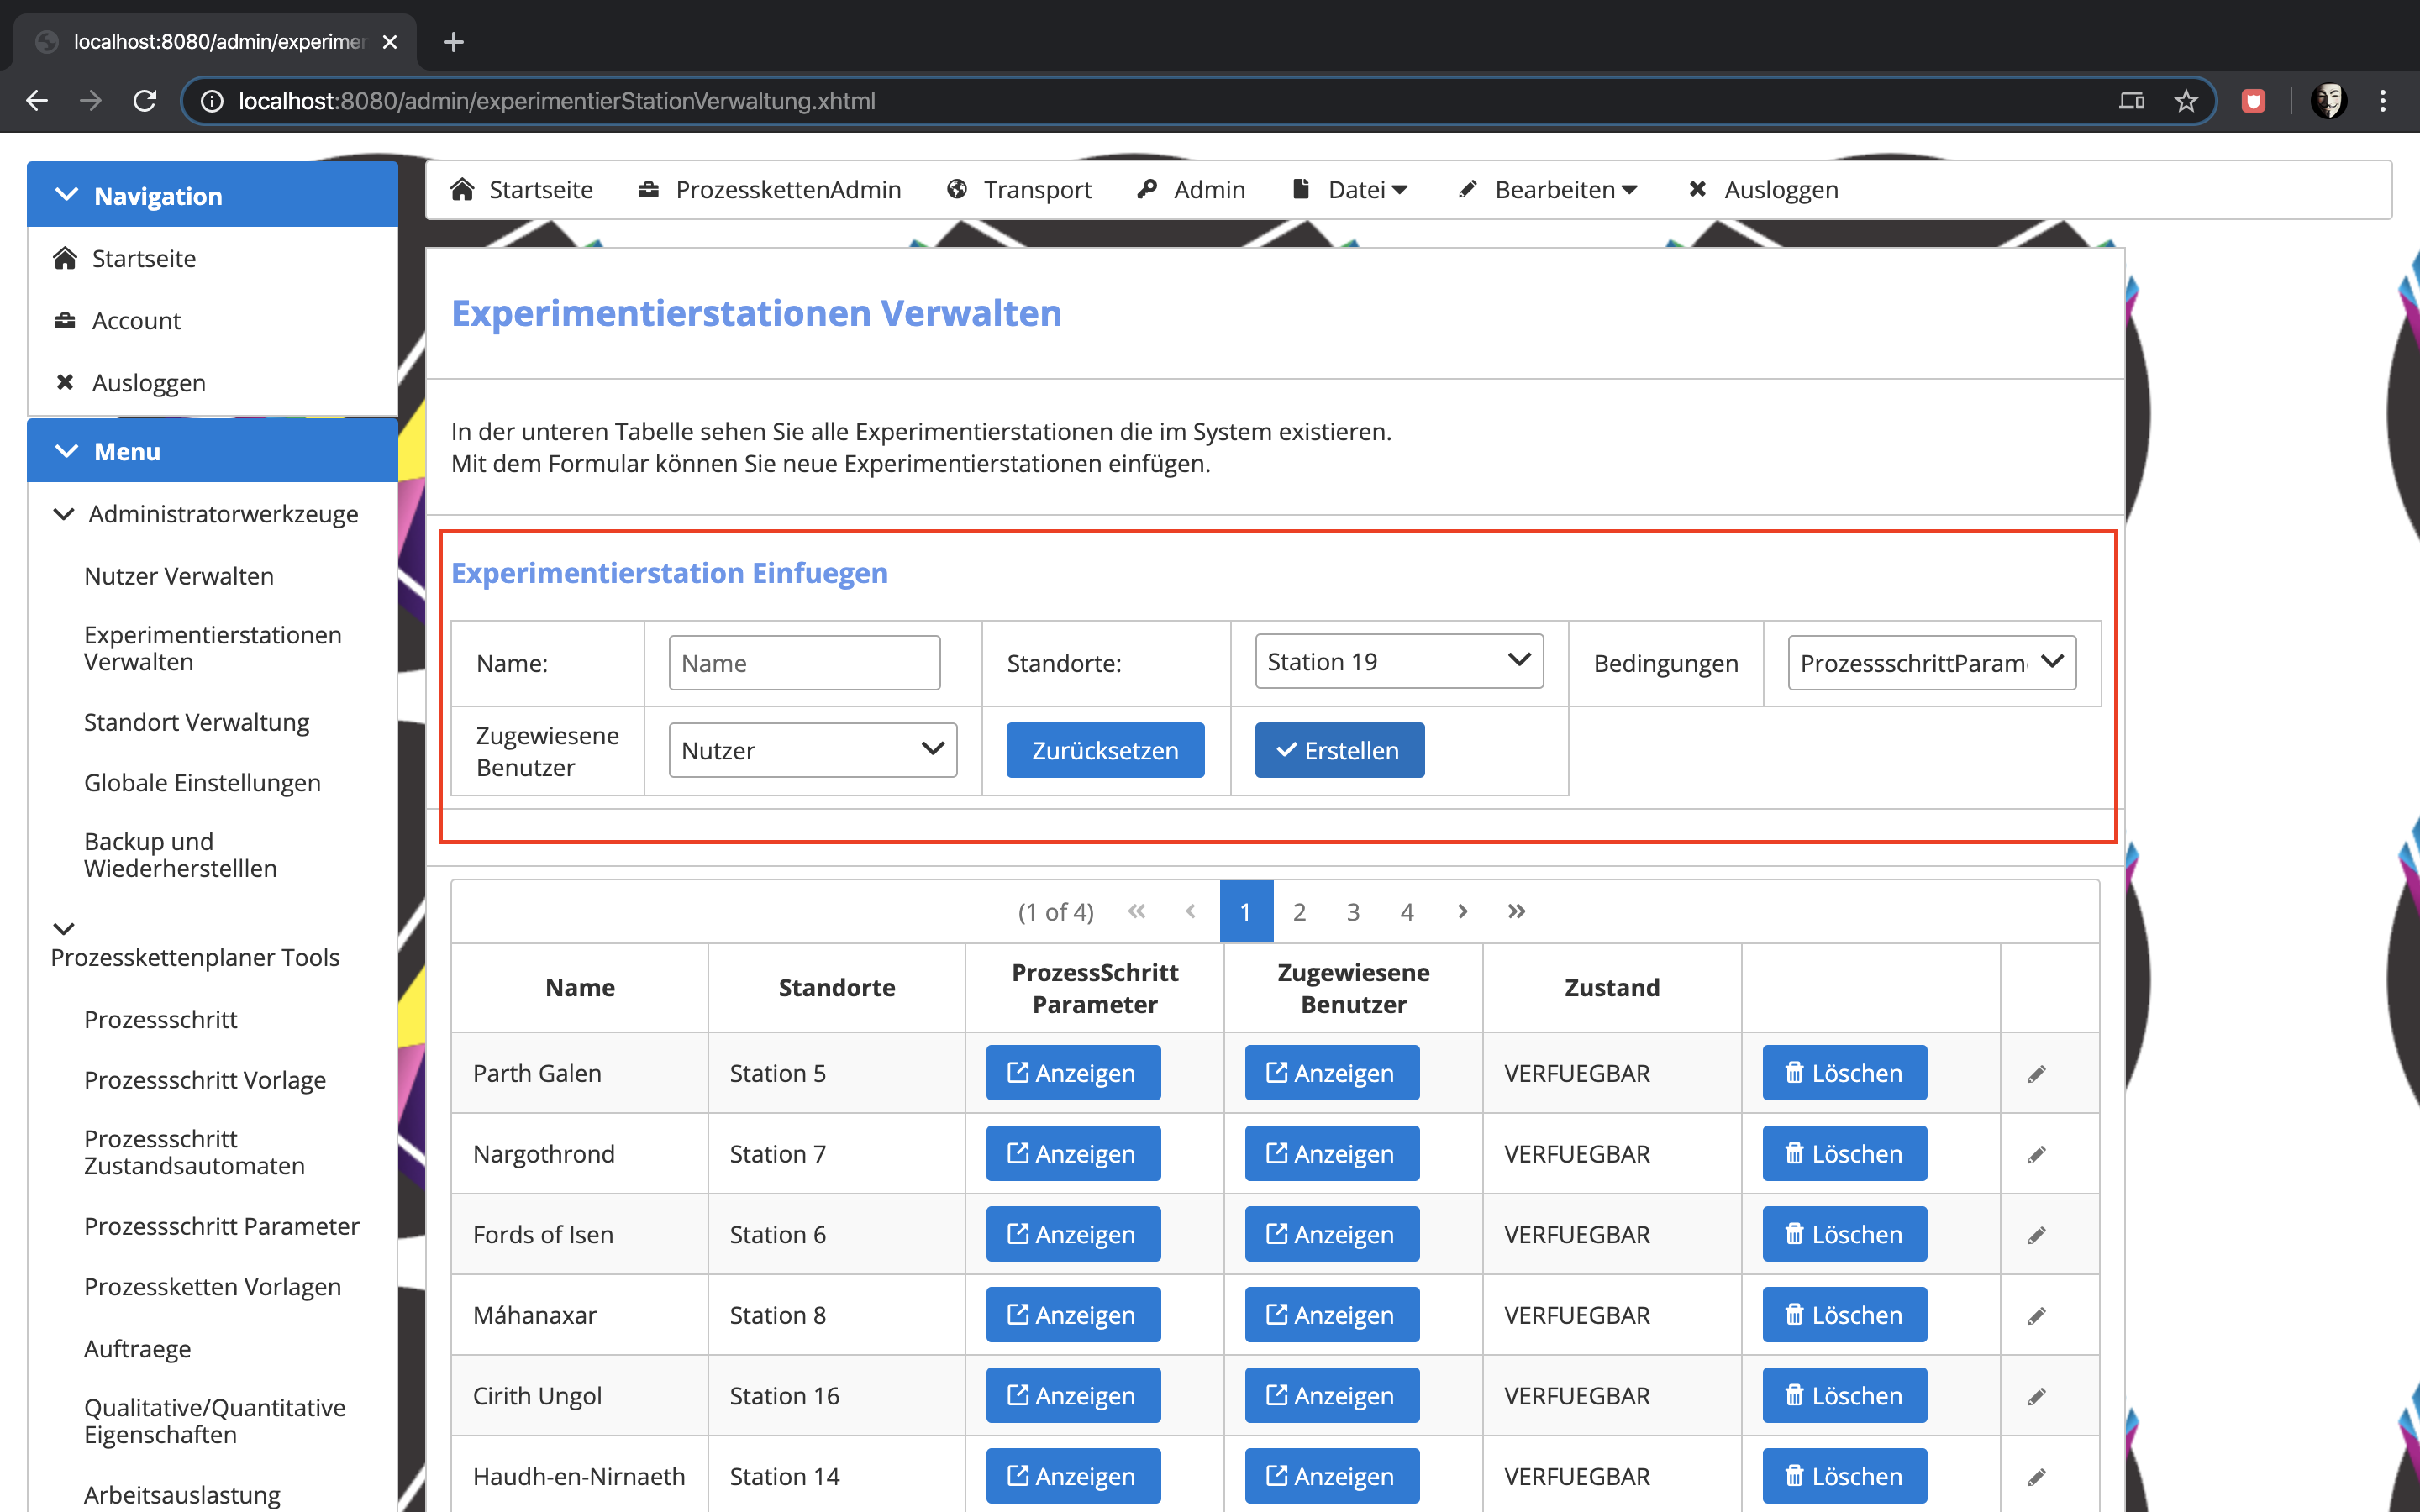
\includegraphics[width=1\textwidth]{Screenshots/3133.png}
\textit{Abbildung 3.2.2.3: Hinzufügen von Experimentierstationen}
} \\

Hier müssen ein beliebiger Name eingegeben und ein Nutzer und ein Standort ausgewählt werden. Dann kann man eine Experimentierstation erstellen. Optional können auch Prozesschrittparameter ausgewählt werden. In diesem Test werde ich alles in die Experimentierstation einfügen (\hyperlink{sc3.1.3.4}{Eingegebene Daten}). 

\hypertarget{sc3.1.3.4}{
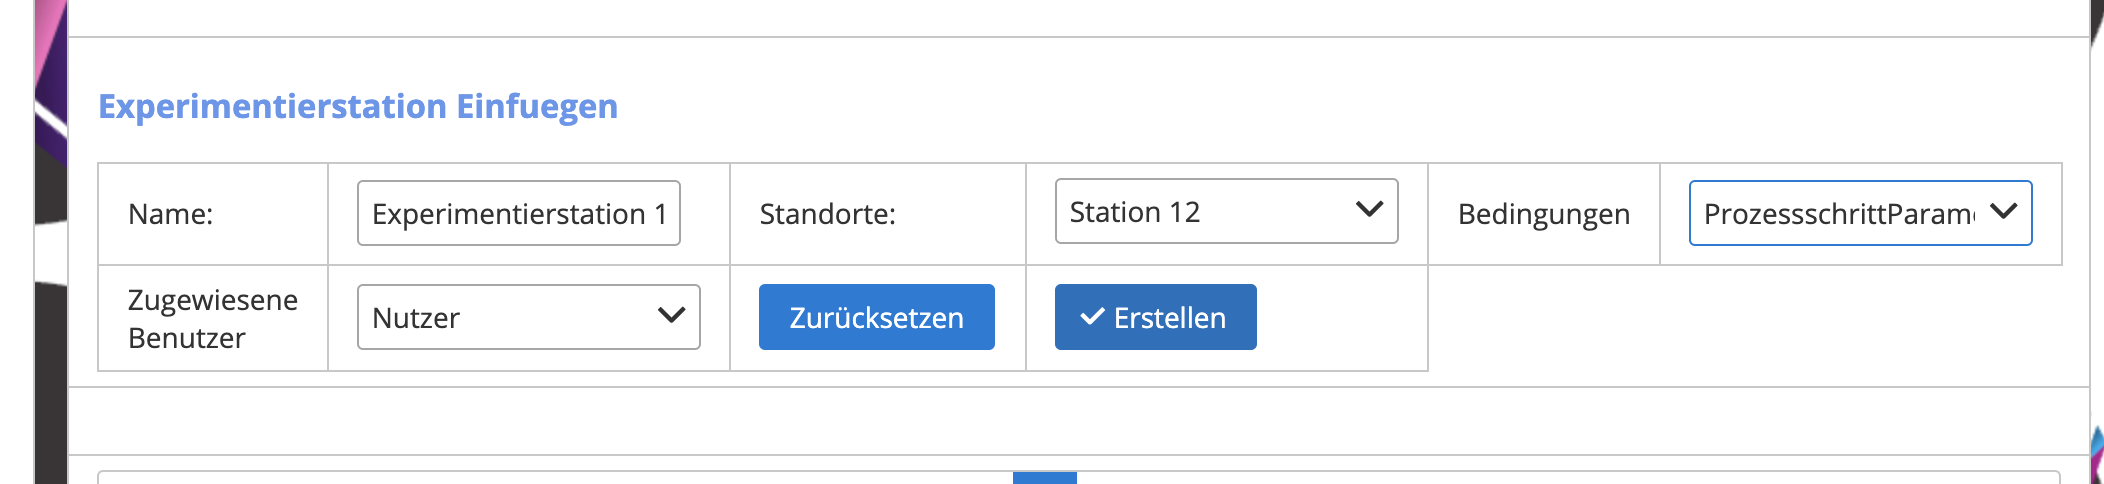
\includegraphics[width=1\textwidth]{Screenshots/3134.png}
\textit{Abbildung 3.2.2.4: Eingegebene Daten}
} \\

Es wurde der \textit{admin} als User zugewiesen und \textit{Sunfyre, Drogon, Meleys und Syrax} als Prozessschrittparameter hinzugefügt. \\

Nun überprüfe ich in der \hyperlink{sc3.1.3.5}{Tabelle}, ob die \textit{Experimentierstation 1} erstellt wurde. \\

\hypertarget{sc3.1.3.5}{
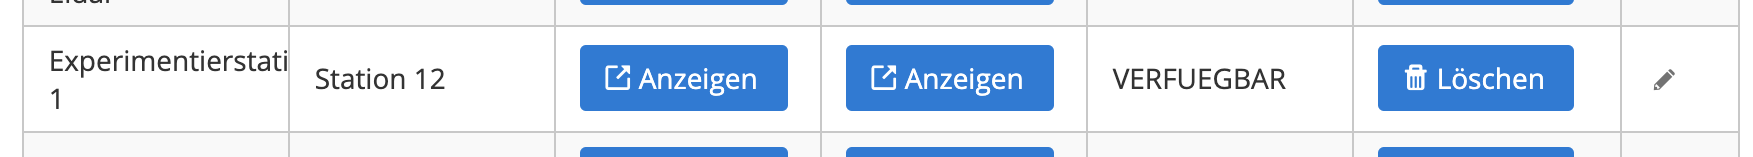
\includegraphics[width=1\textwidth]{Screenshots/3135.png}
\textit{Abbildung 3.2.2.5: Eben erstellte Daten in der Tabelle}
} \\

Wenn man in der Tabelle in der richtigen Zeile auf \hyperlink{sc3.1.3.6}{Anzeigen der Prozessschrittparameter} drückt, dann öffnet sich ein Menü, indem in einer Tabelle alle zugewiesenen Prozessparameter angezeigt werden. \\

\hypertarget{sc3.1.3.6}{
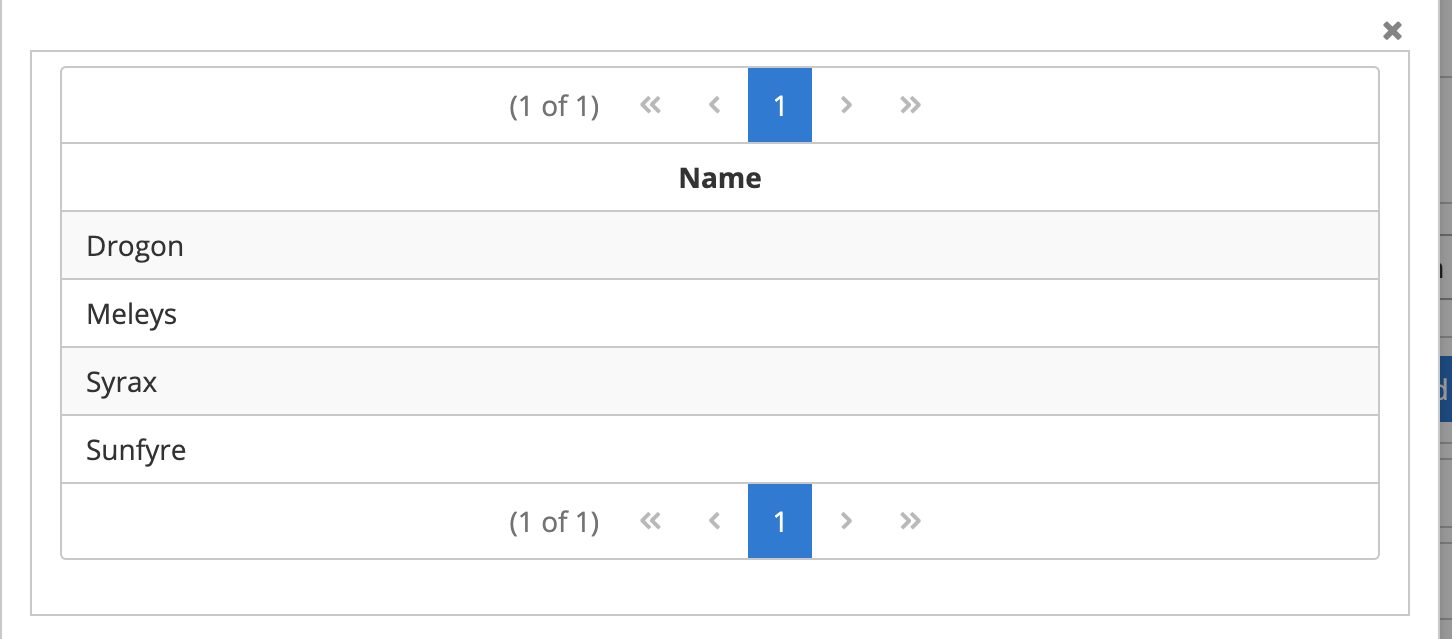
\includegraphics[width=1\textwidth]{Screenshots/3136.png}
\textit{Abbildung 3.2.2.6: Zugewiesene Prozessparameter}
} \\

Gleiches passiert wenn man \hyperlink{sc3.1.3.7}{Anzeigen der zugewiesenen Benutzer} drückt. 

\hypertarget{sc3.1.3.7}{
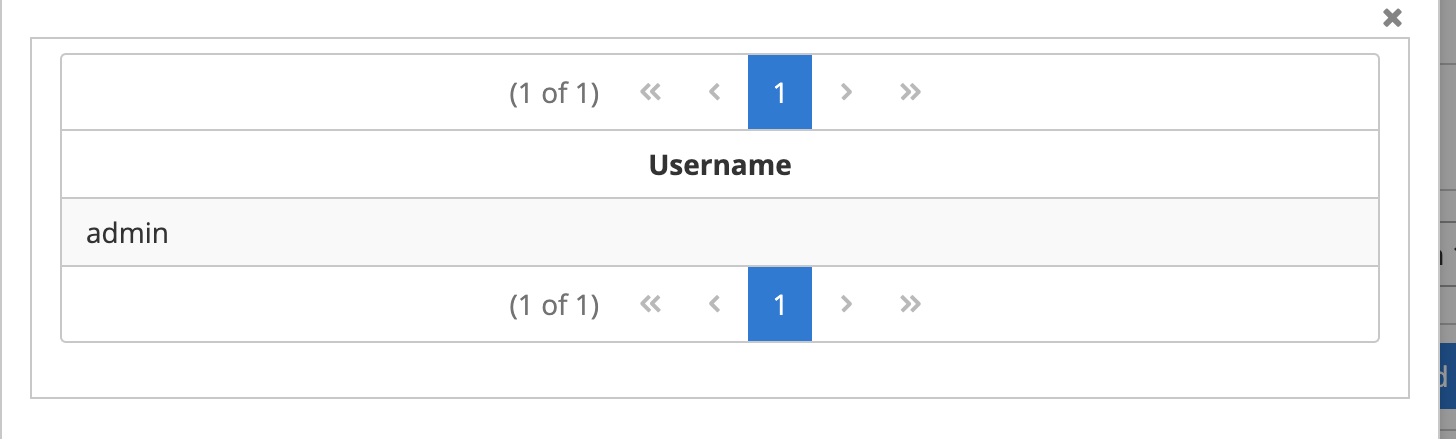
\includegraphics[width=1\textwidth]{Screenshots/3137.png}
\textit{Abbildung 3.2.2.7: Zugewiesene Benutzer}
} \\

Die Tests für das Hinzufügen und das Einsehen von Experimentierstationen verliefen erfolgreich. 

\paragraph{Bearbeiten von existierenden Experimentierstationen:} 


Die zu bearbeitende Experimentierstation heißt \hyperlink{sc3.1.3.8}{ES2}. Sie hat folgende \hyperlink{sc3.1.3.9}{Prozessschrittparameter} und \hyperlink{sc3.1.3.10}{Benutzer} zugewiesen\\

\hypertarget{sc3.1.3.8}{
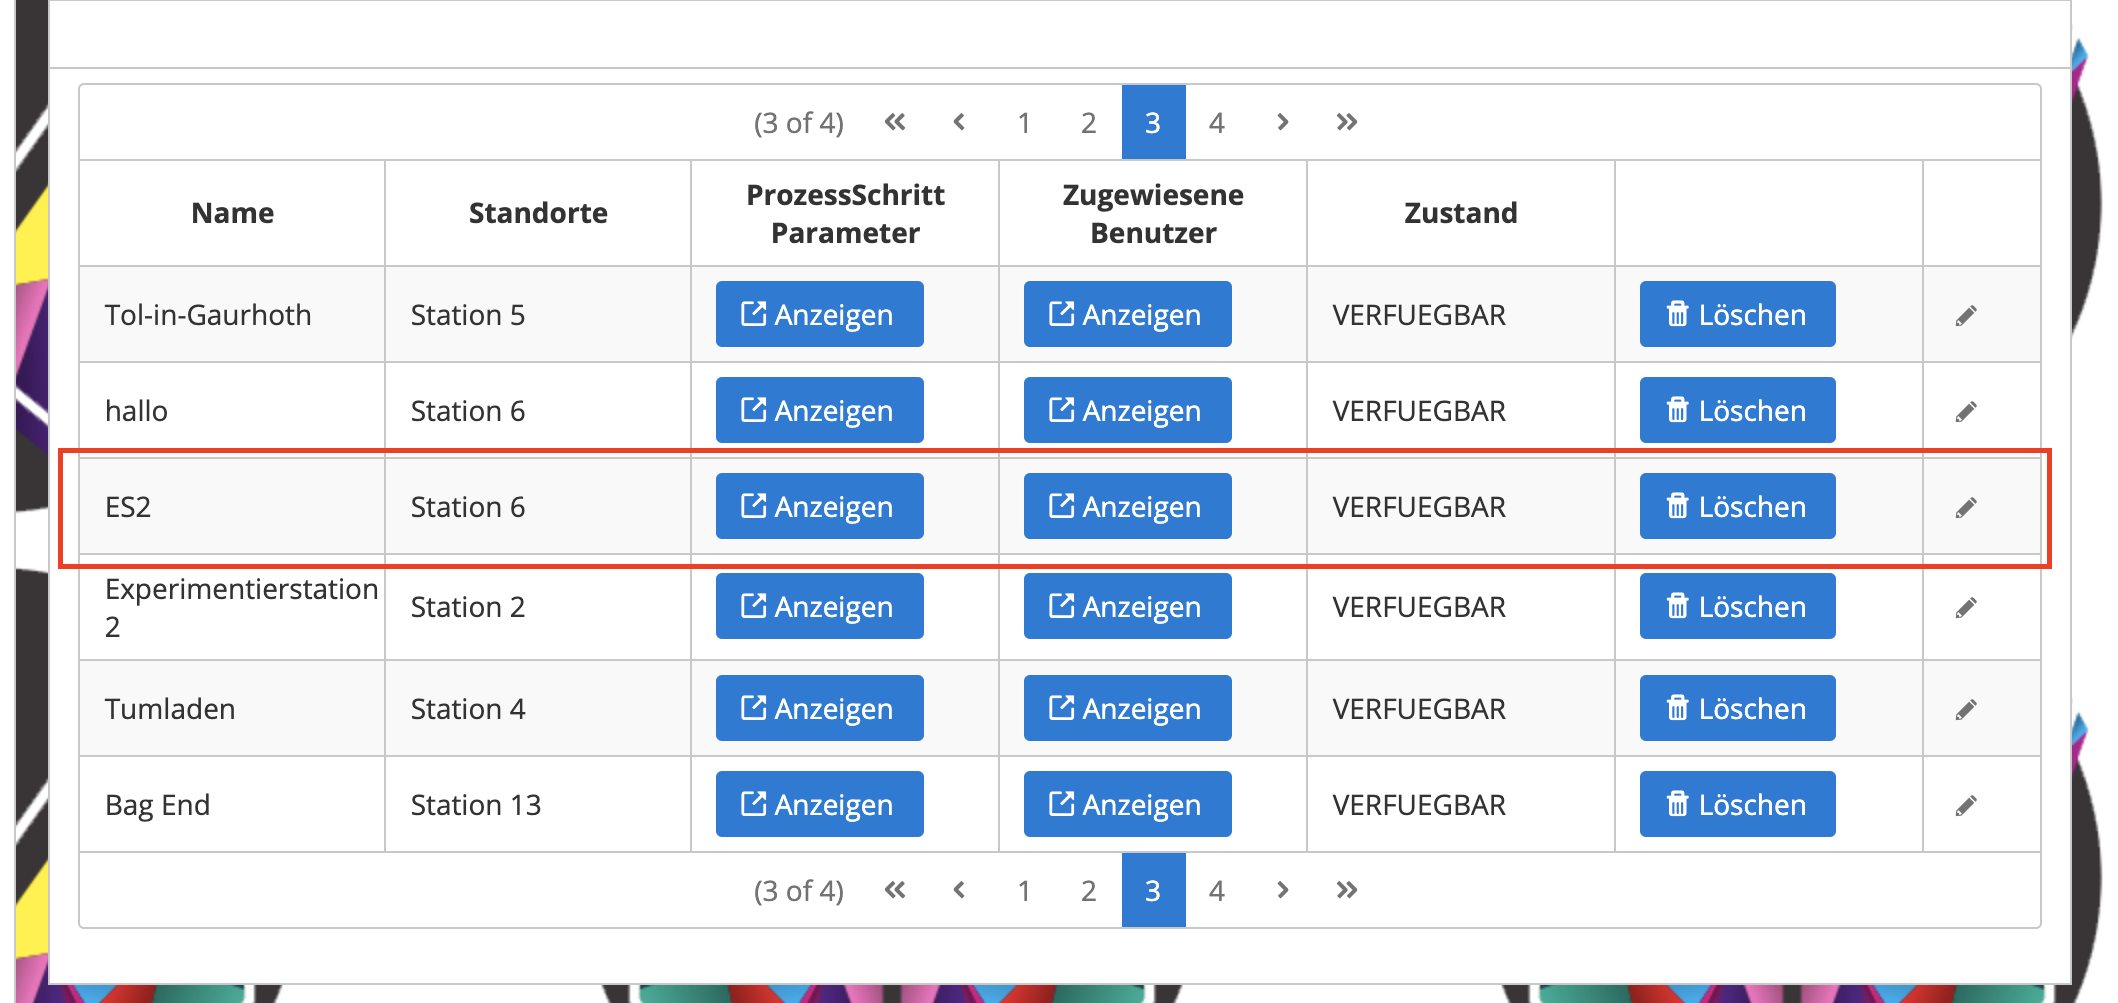
\includegraphics[width=1\textwidth]{Screenshots/3138.png}
\textit{Abbildung 3.2.2.8: Zu bearbeitende Experimentierstation}
} \\

\hypertarget{sc3.1.3.9}{
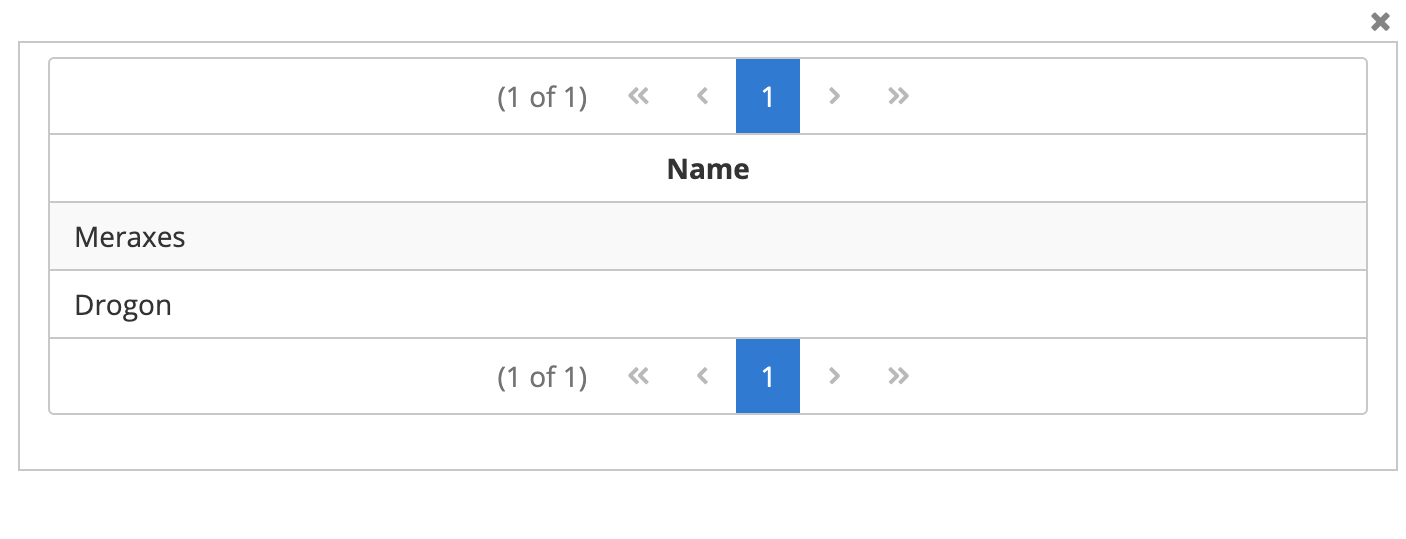
\includegraphics[width=1\textwidth]{Screenshots/3139.png}
\textit{Abbildung 3.2.2.9: Prozessschrittparameter der zu bearbeitende Experimentierstation}
} \\

\hypertarget{sc3.1.3.10}{
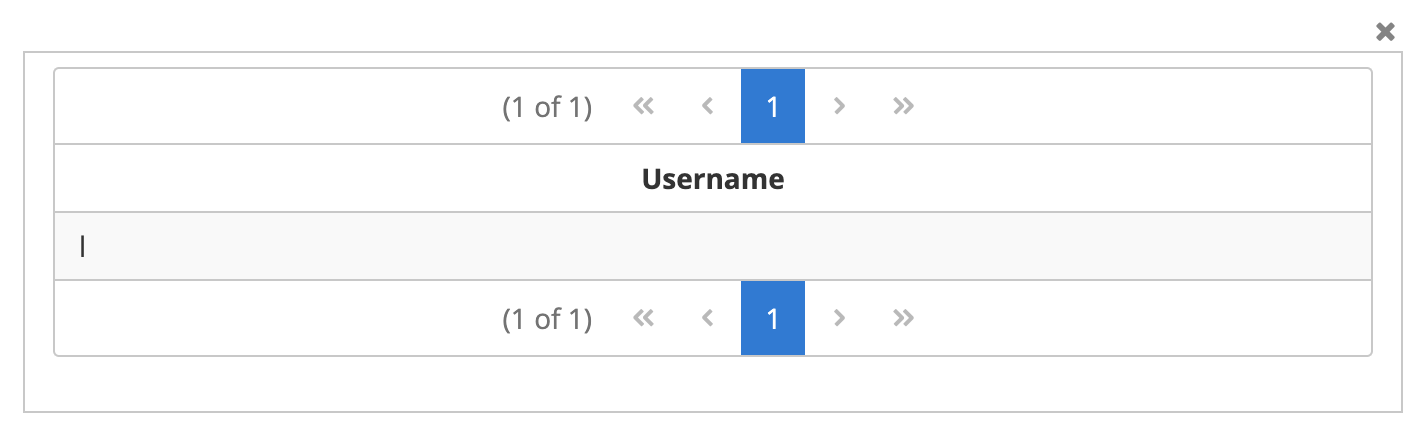
\includegraphics[width=1\textwidth]{Screenshots/31310.png}
\textit{Abbildung 3.2.2.10: Benutzer der zu bearbeitende Experimentierstation}
} \\

Jetzt wollen wir den Benutzer \textit{l} entfernen und den Benutzer \textit{t} hinzufügen. Hierfür gehen wir in der Zeile von ES2 auf den  \hyperlink{sc3.1.3.11}{Stift zum Bearbeiten} und öffnen das Ausklappfenster in der Spalte der zugewiesenen Benutzer. Hier wählen wir den neuen Benutzer aus und drücken rechts auf den Haken um zu speichern. \\

\hypertarget{sc3.1.3.11}{
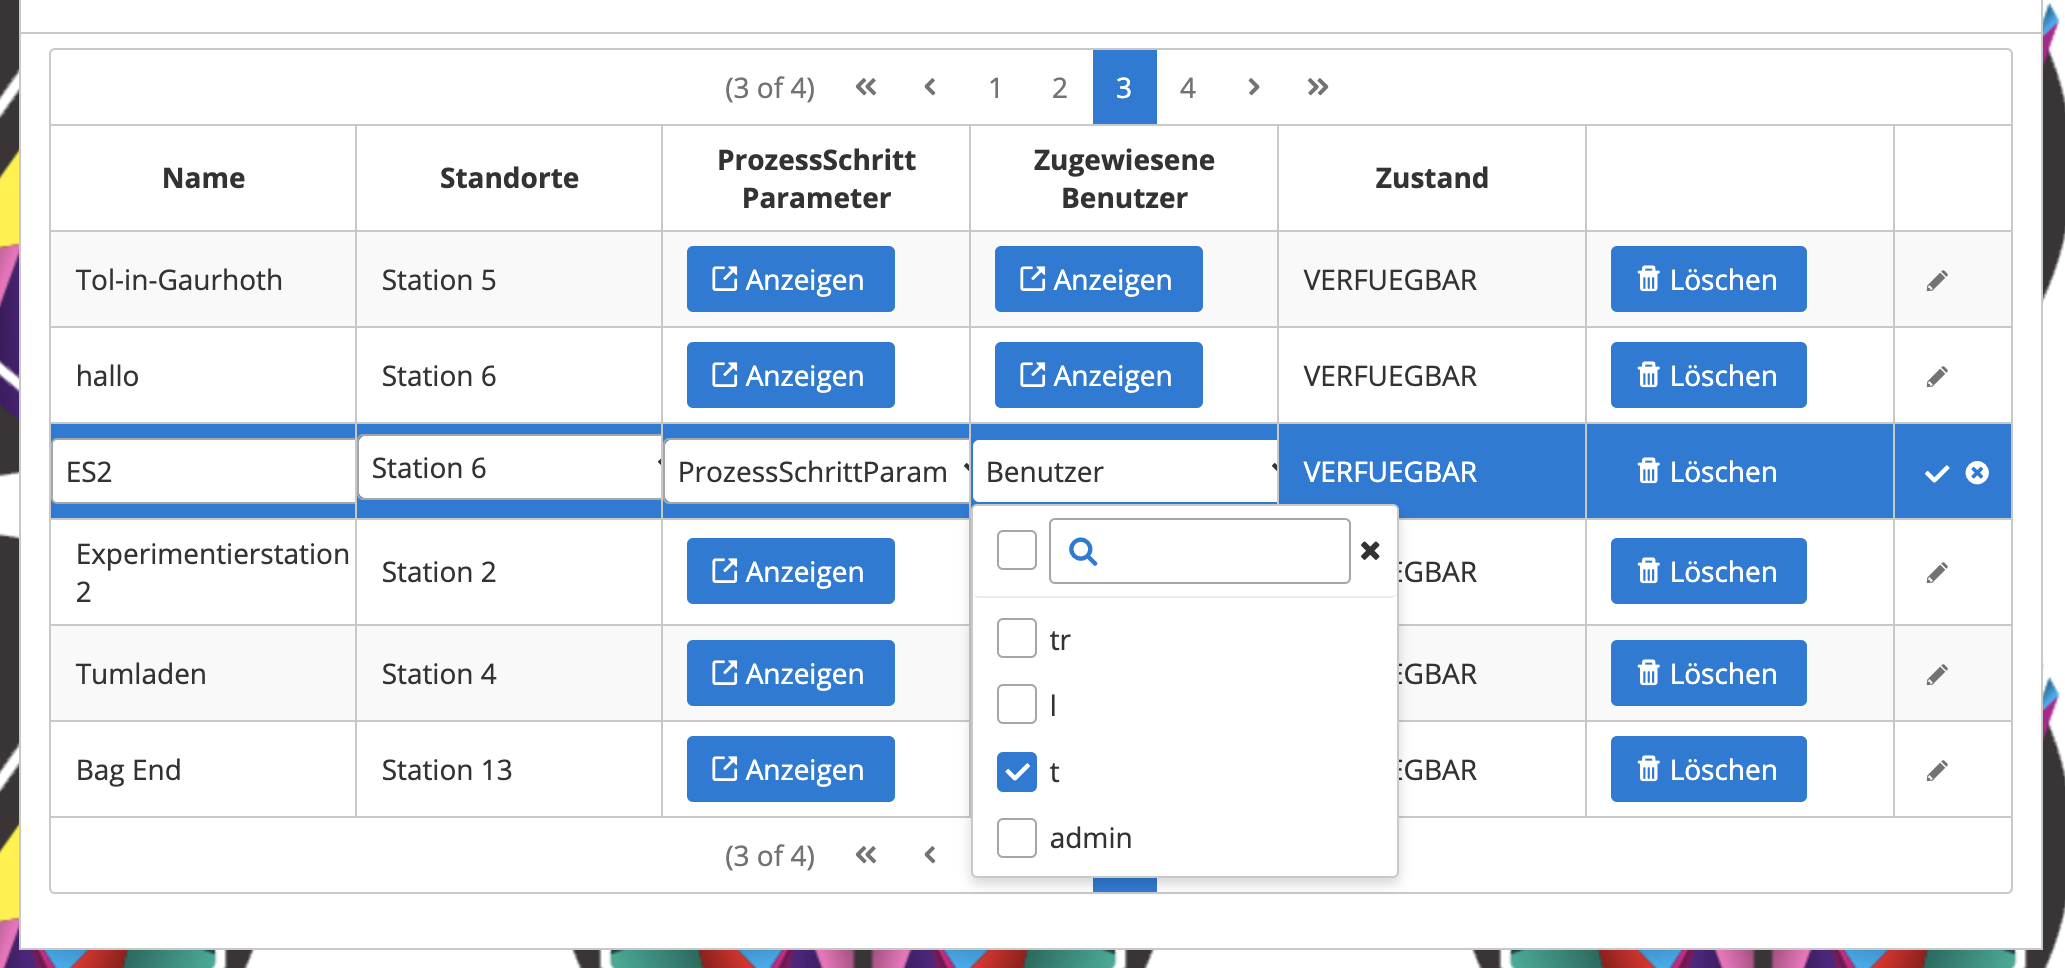
\includegraphics[width=1\textwidth]{Screenshots/31311.png}
\textit{Abbildung 3.2.2.11: Benutzer bearbeiten}
} \\

Anschließend sieht man in der \hyperlink{sc3.1.3.12}{Tabelle} in dem \textit{Anzeigen}-Menü, dass der Benutzer gewechselt wurde.\\

\hypertarget{sc3.1.3.12}{
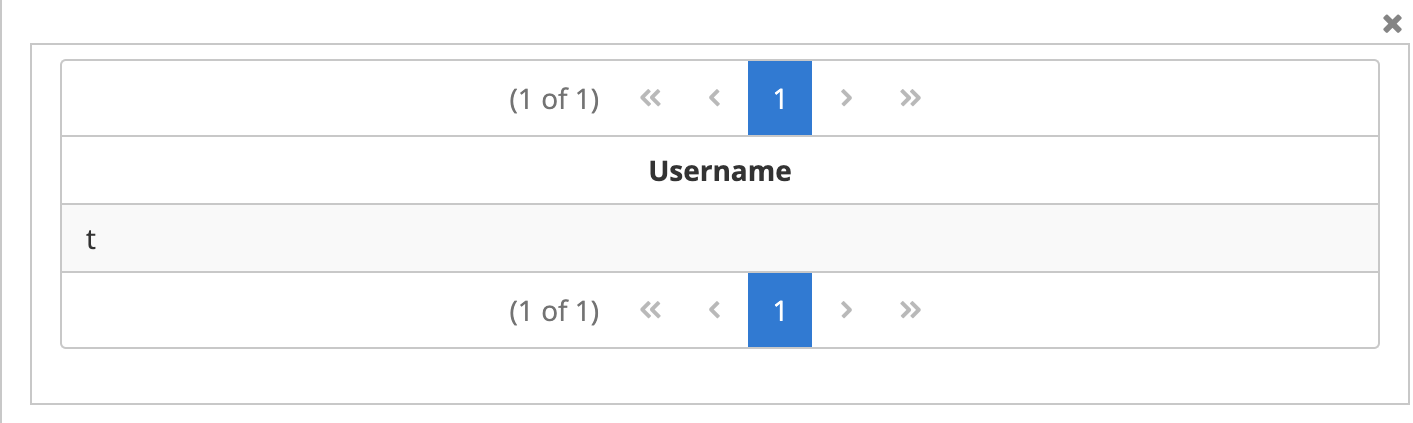
\includegraphics[width=1\textwidth]{Screenshots/31312.png}
\textit{Abbildung 3.2.2.12: Benutzer bearteitet}
} \\

Der Test verlief erfolgreich. die Tests für das bearbeiten von Name, Standort und Prozessschrittparameter wurde analog zu diesem getestet und waren ebenfalls erfolgreich.

\paragraph{Löschen von Experimentierstationen:}


Nun werde ich die Experimentierstation mit dem Namen \textit{Experimentierstation 2} löschen. Hierzu gehe ich in der Tabelle in der entsprechenden Zeile auf  \hyperlink{sc3.1.3.13}{löschen}, und die Experimentierstation wird gelöscht.\\

\hypertarget{sc3.1.3.13}{
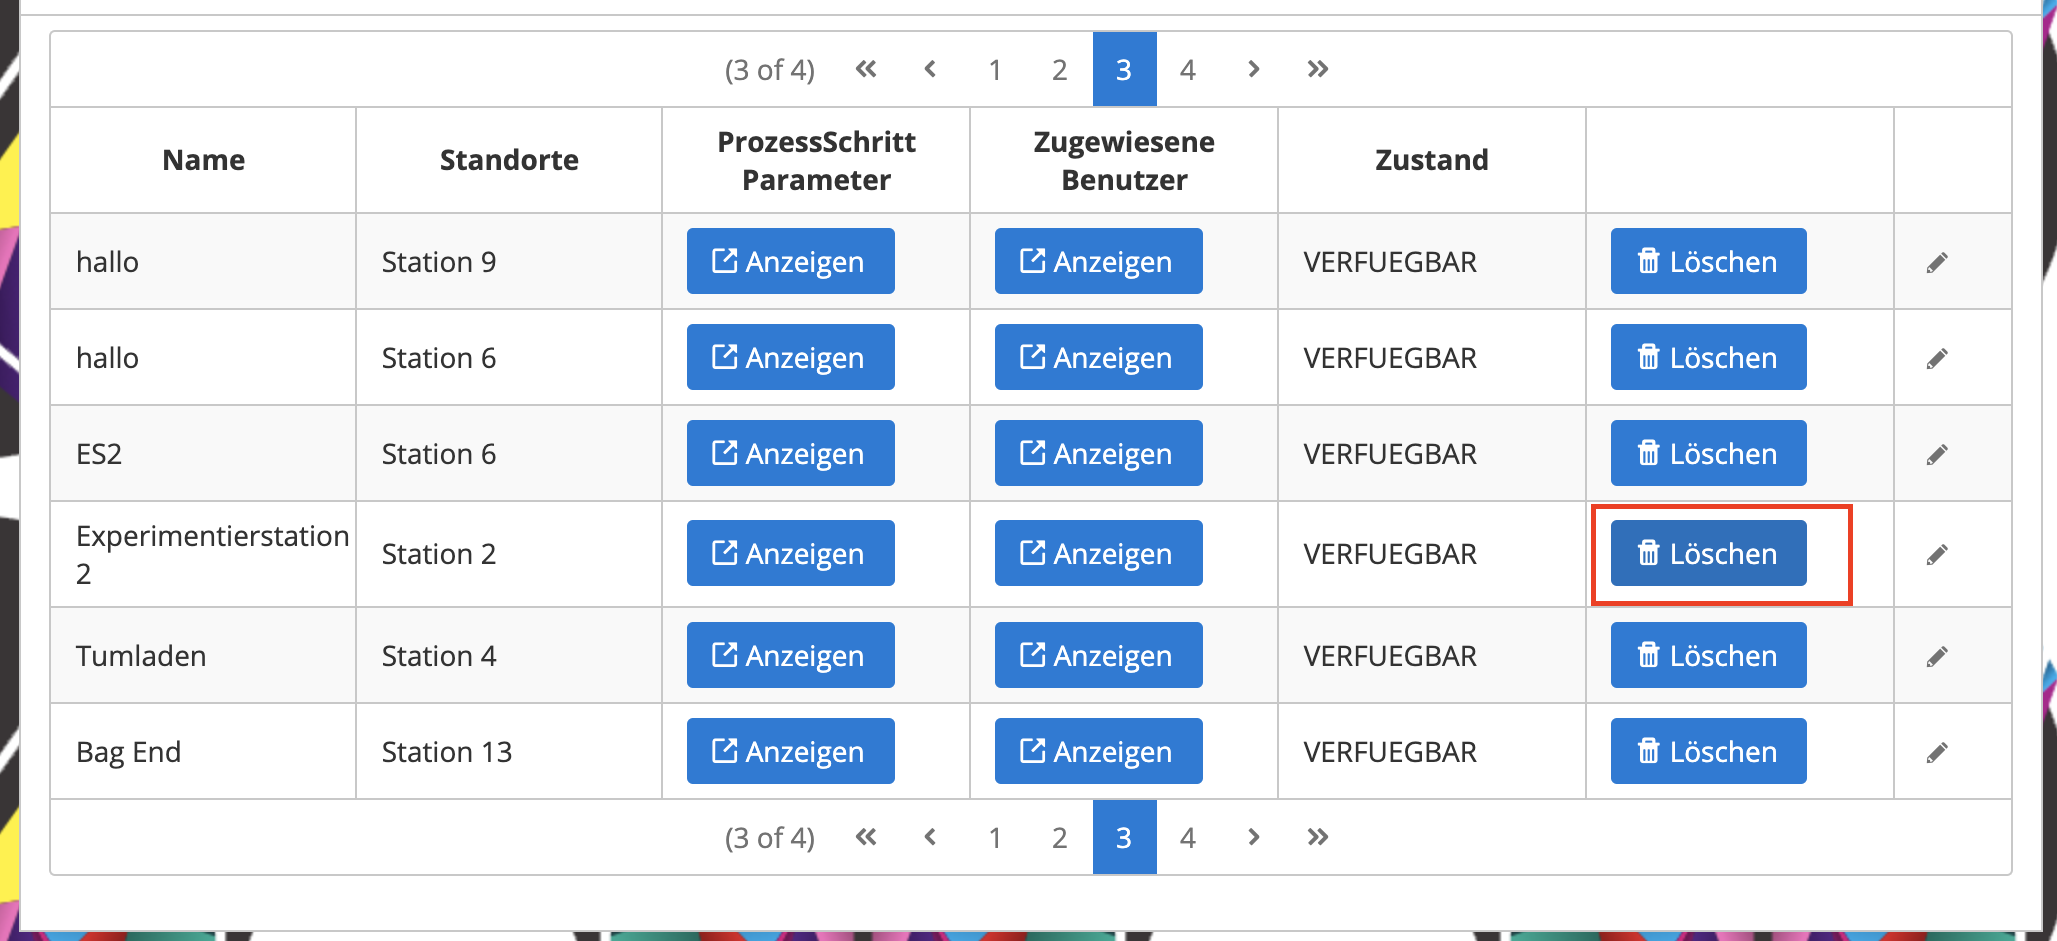
\includegraphics[width=1\textwidth]{Screenshots/31313.png}
\textit{Abbildung 3.2.2.13: Experimentierstation löschen}
} \\

\hypertarget{sc3.1.3.14}{
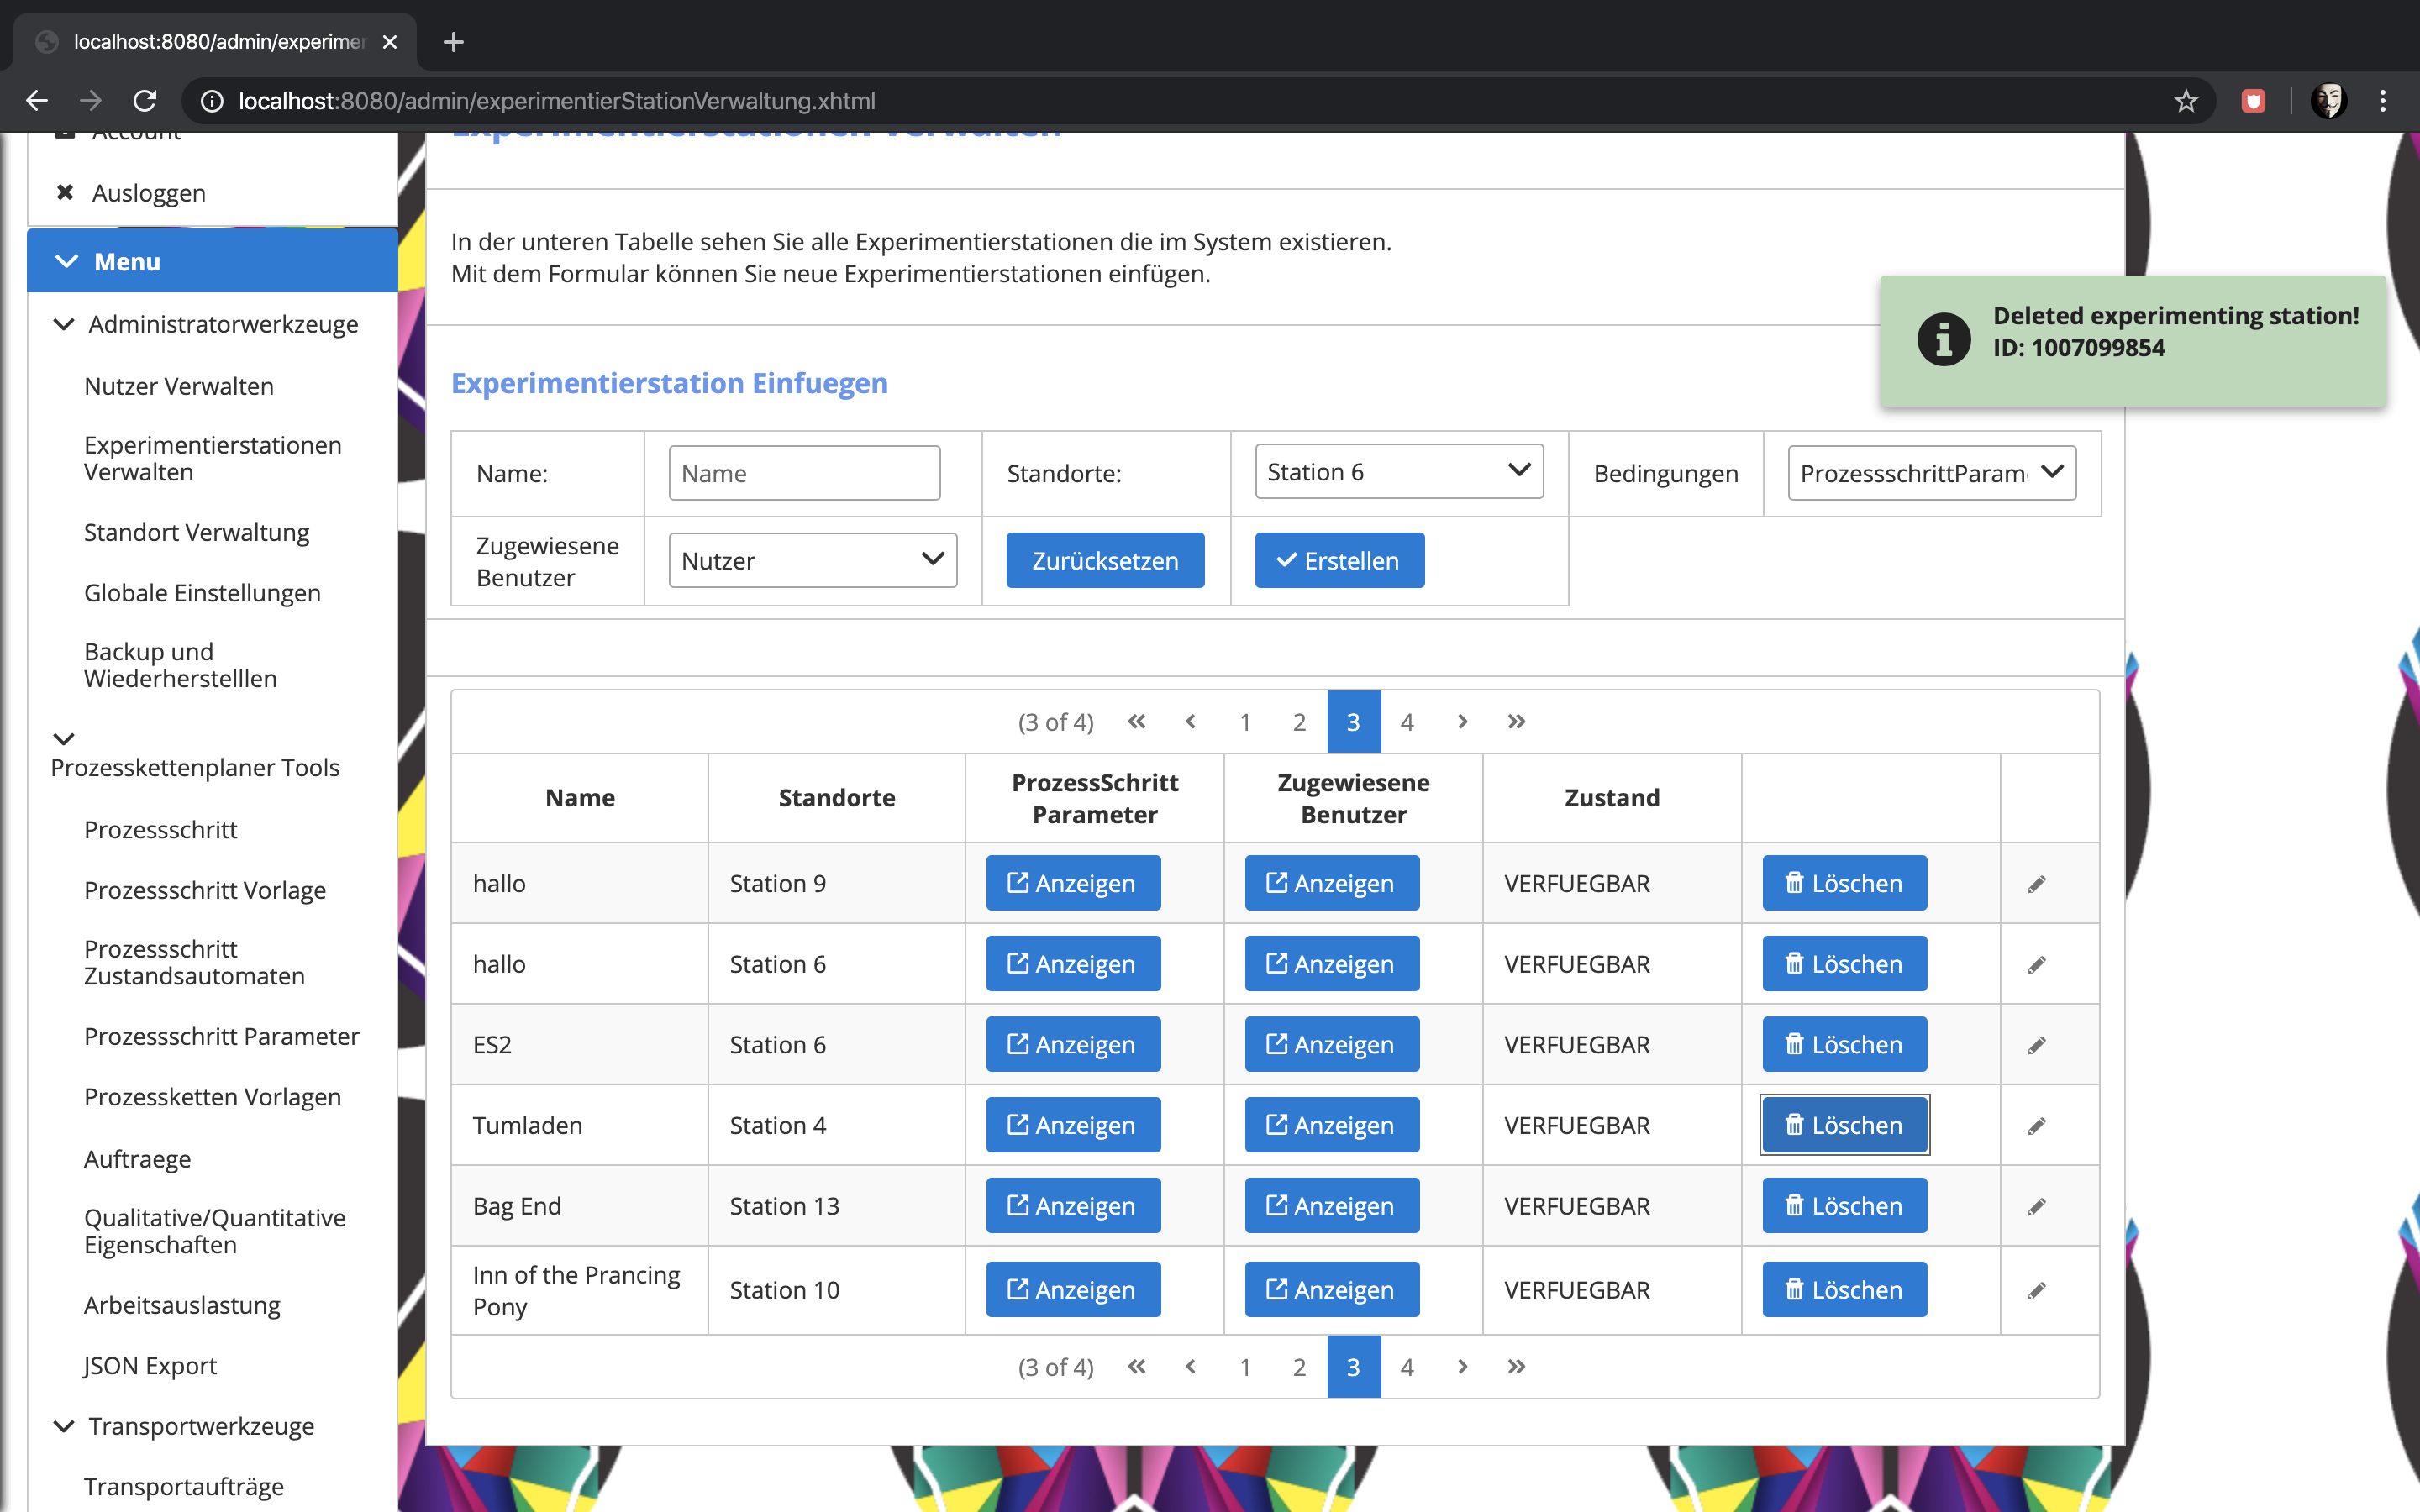
\includegraphics[width=1\textwidth]{Screenshots/31314.png}
\textit{Abbildung 3.2.2.14: Experimentierstation gelöscht}
} \\

\hyperlink{sc3.1.3.14}{Hier} sieht man eine Löschbestätigung oben rechts in der Ecke und der Eintrag wurde aus der Tabelle gelöscht. Auch nach einem erneuten Laden der Seite bleibt sie gelöscht. Also ist auch dieser Test erfolgreich. 

%%

\subsubsection{Anwendungsfall: Standort Test per Hand}

Der Administrator kann über ein Formular mit dem Standort auf der entsprechenden Website interagieren. Auf der entsprechenden Website kann der Benutzer den Standort anzeigen, ändern und löschen.\\

\hypertarget{sc3.1.4.1}{
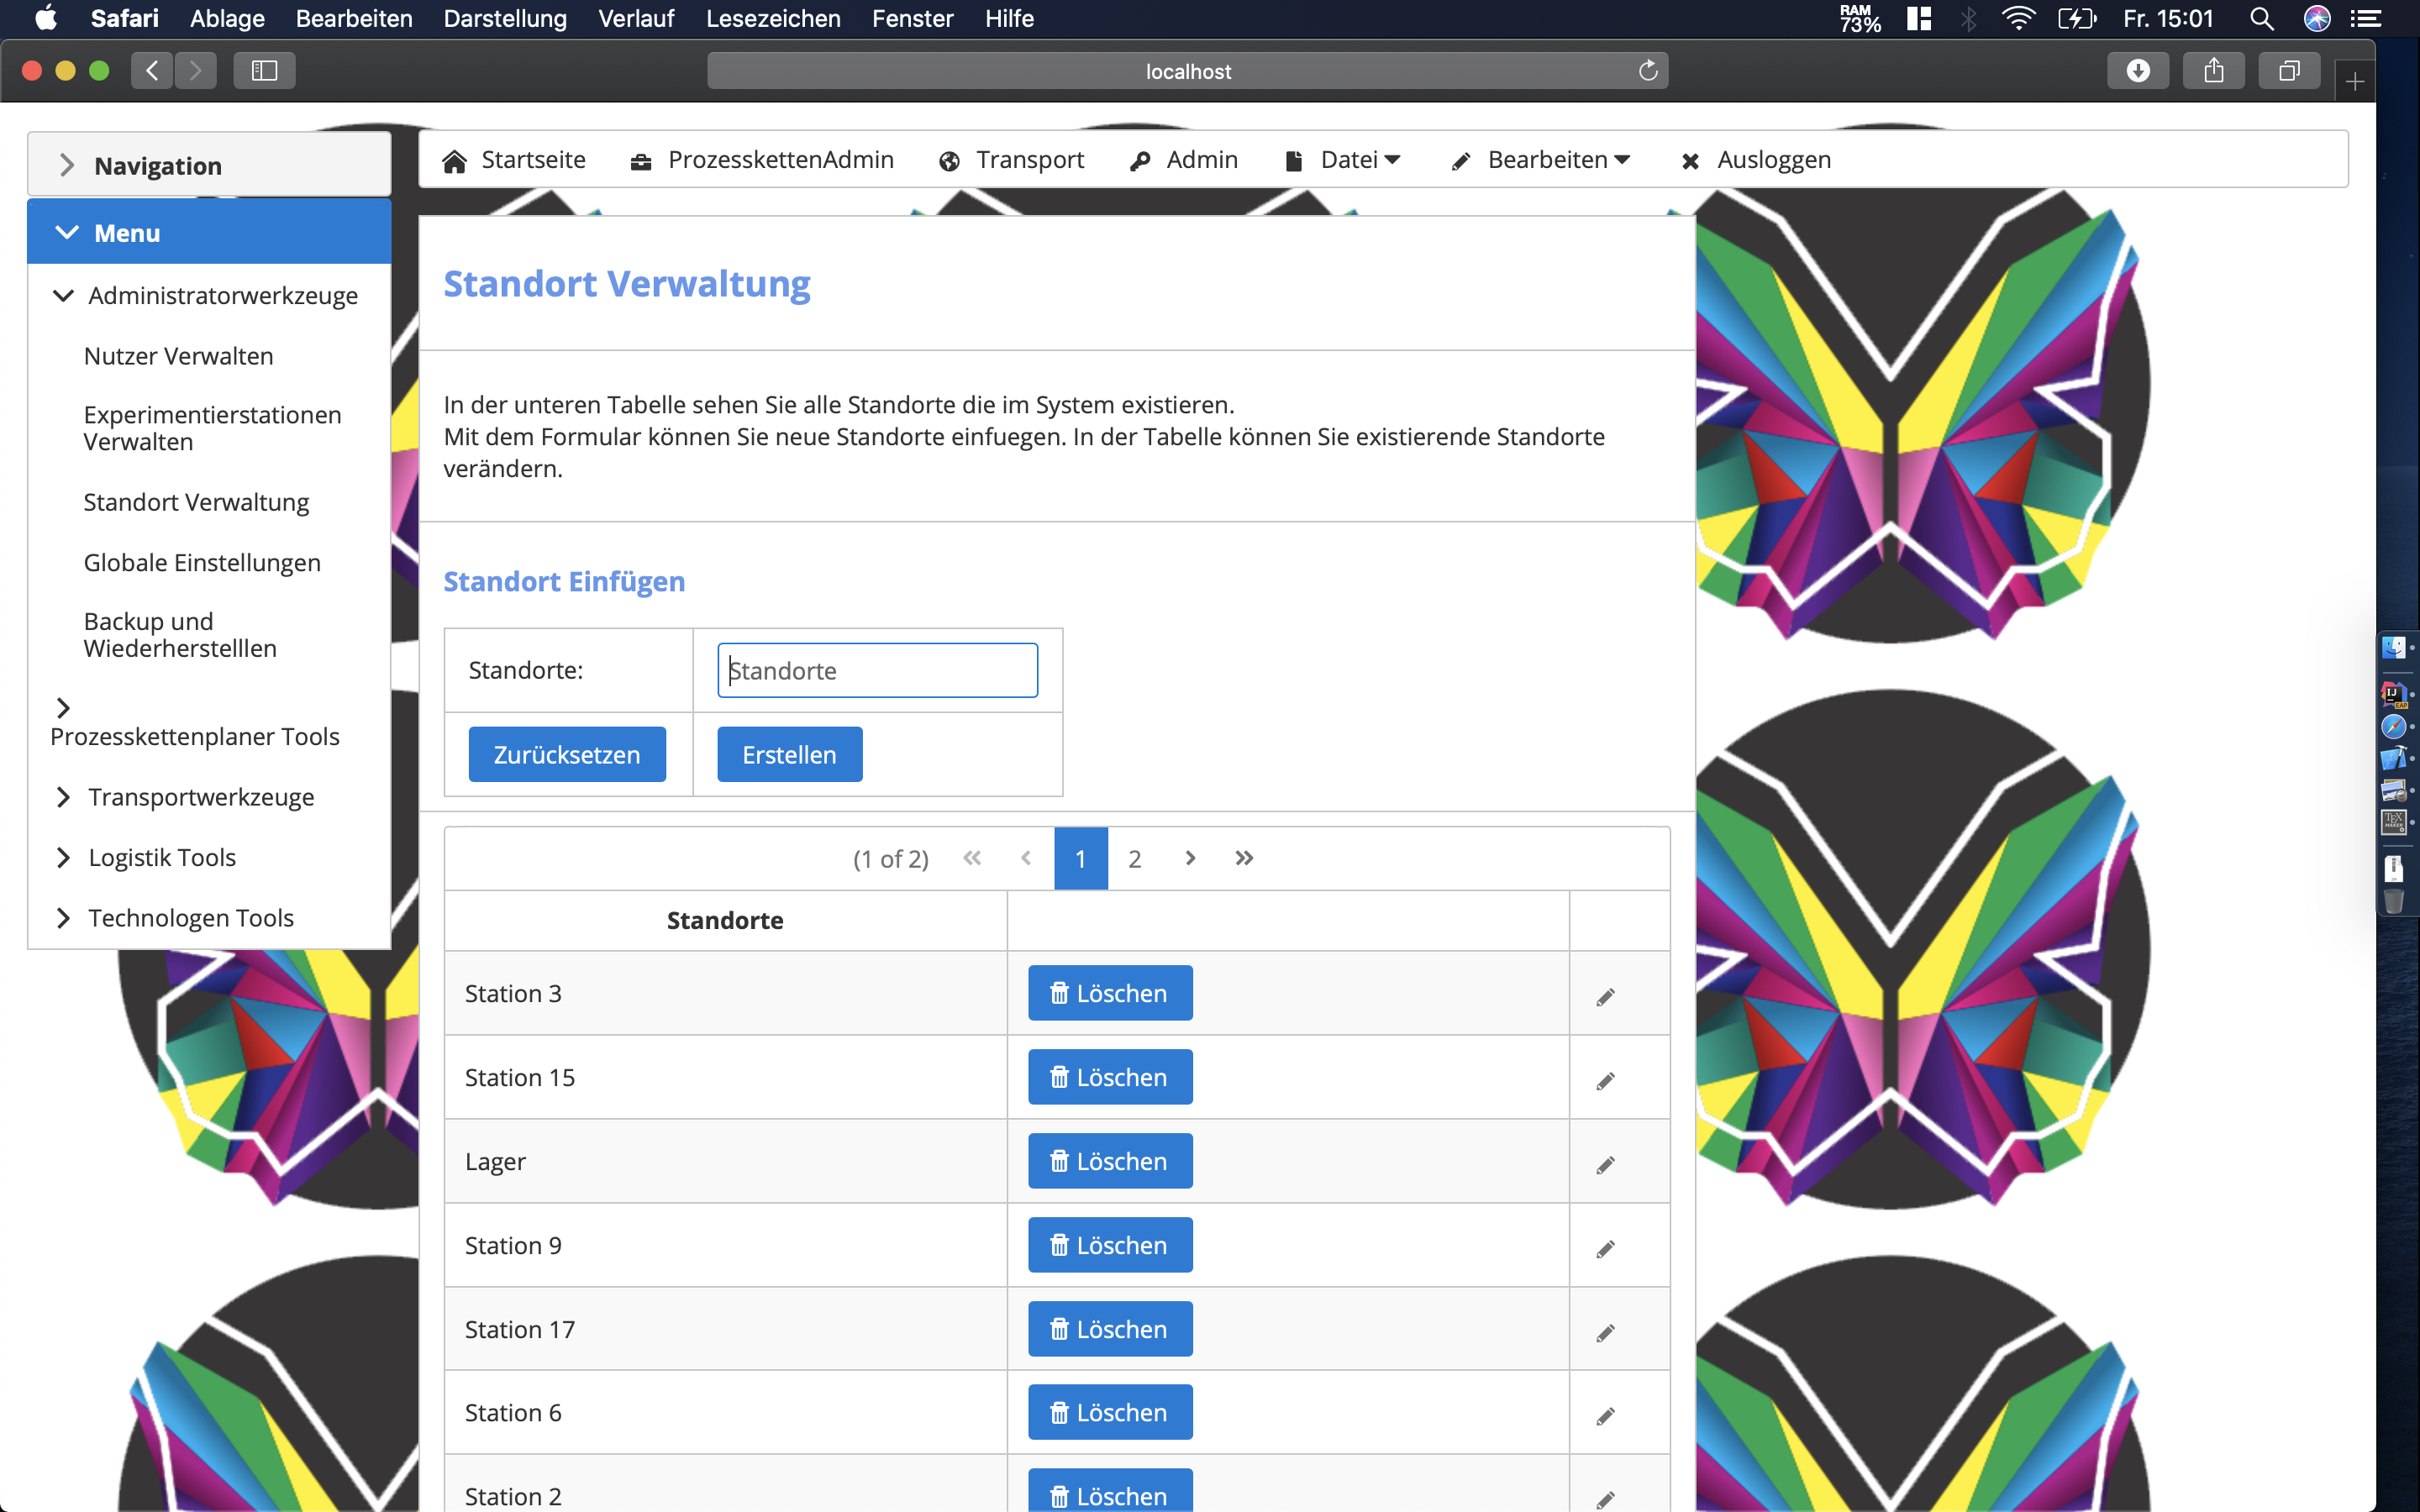
\includegraphics[width=1\textwidth]{Screenshots/4StandOrtFormular.png}
\textit{Abbildung 3.2.3.1: Standort Formular}
} \\

Wenn ein Standort erstellt wird, wird eine Bestätigungsnachricht empfangen.\\

\hypertarget{sc3.1.4.2}{
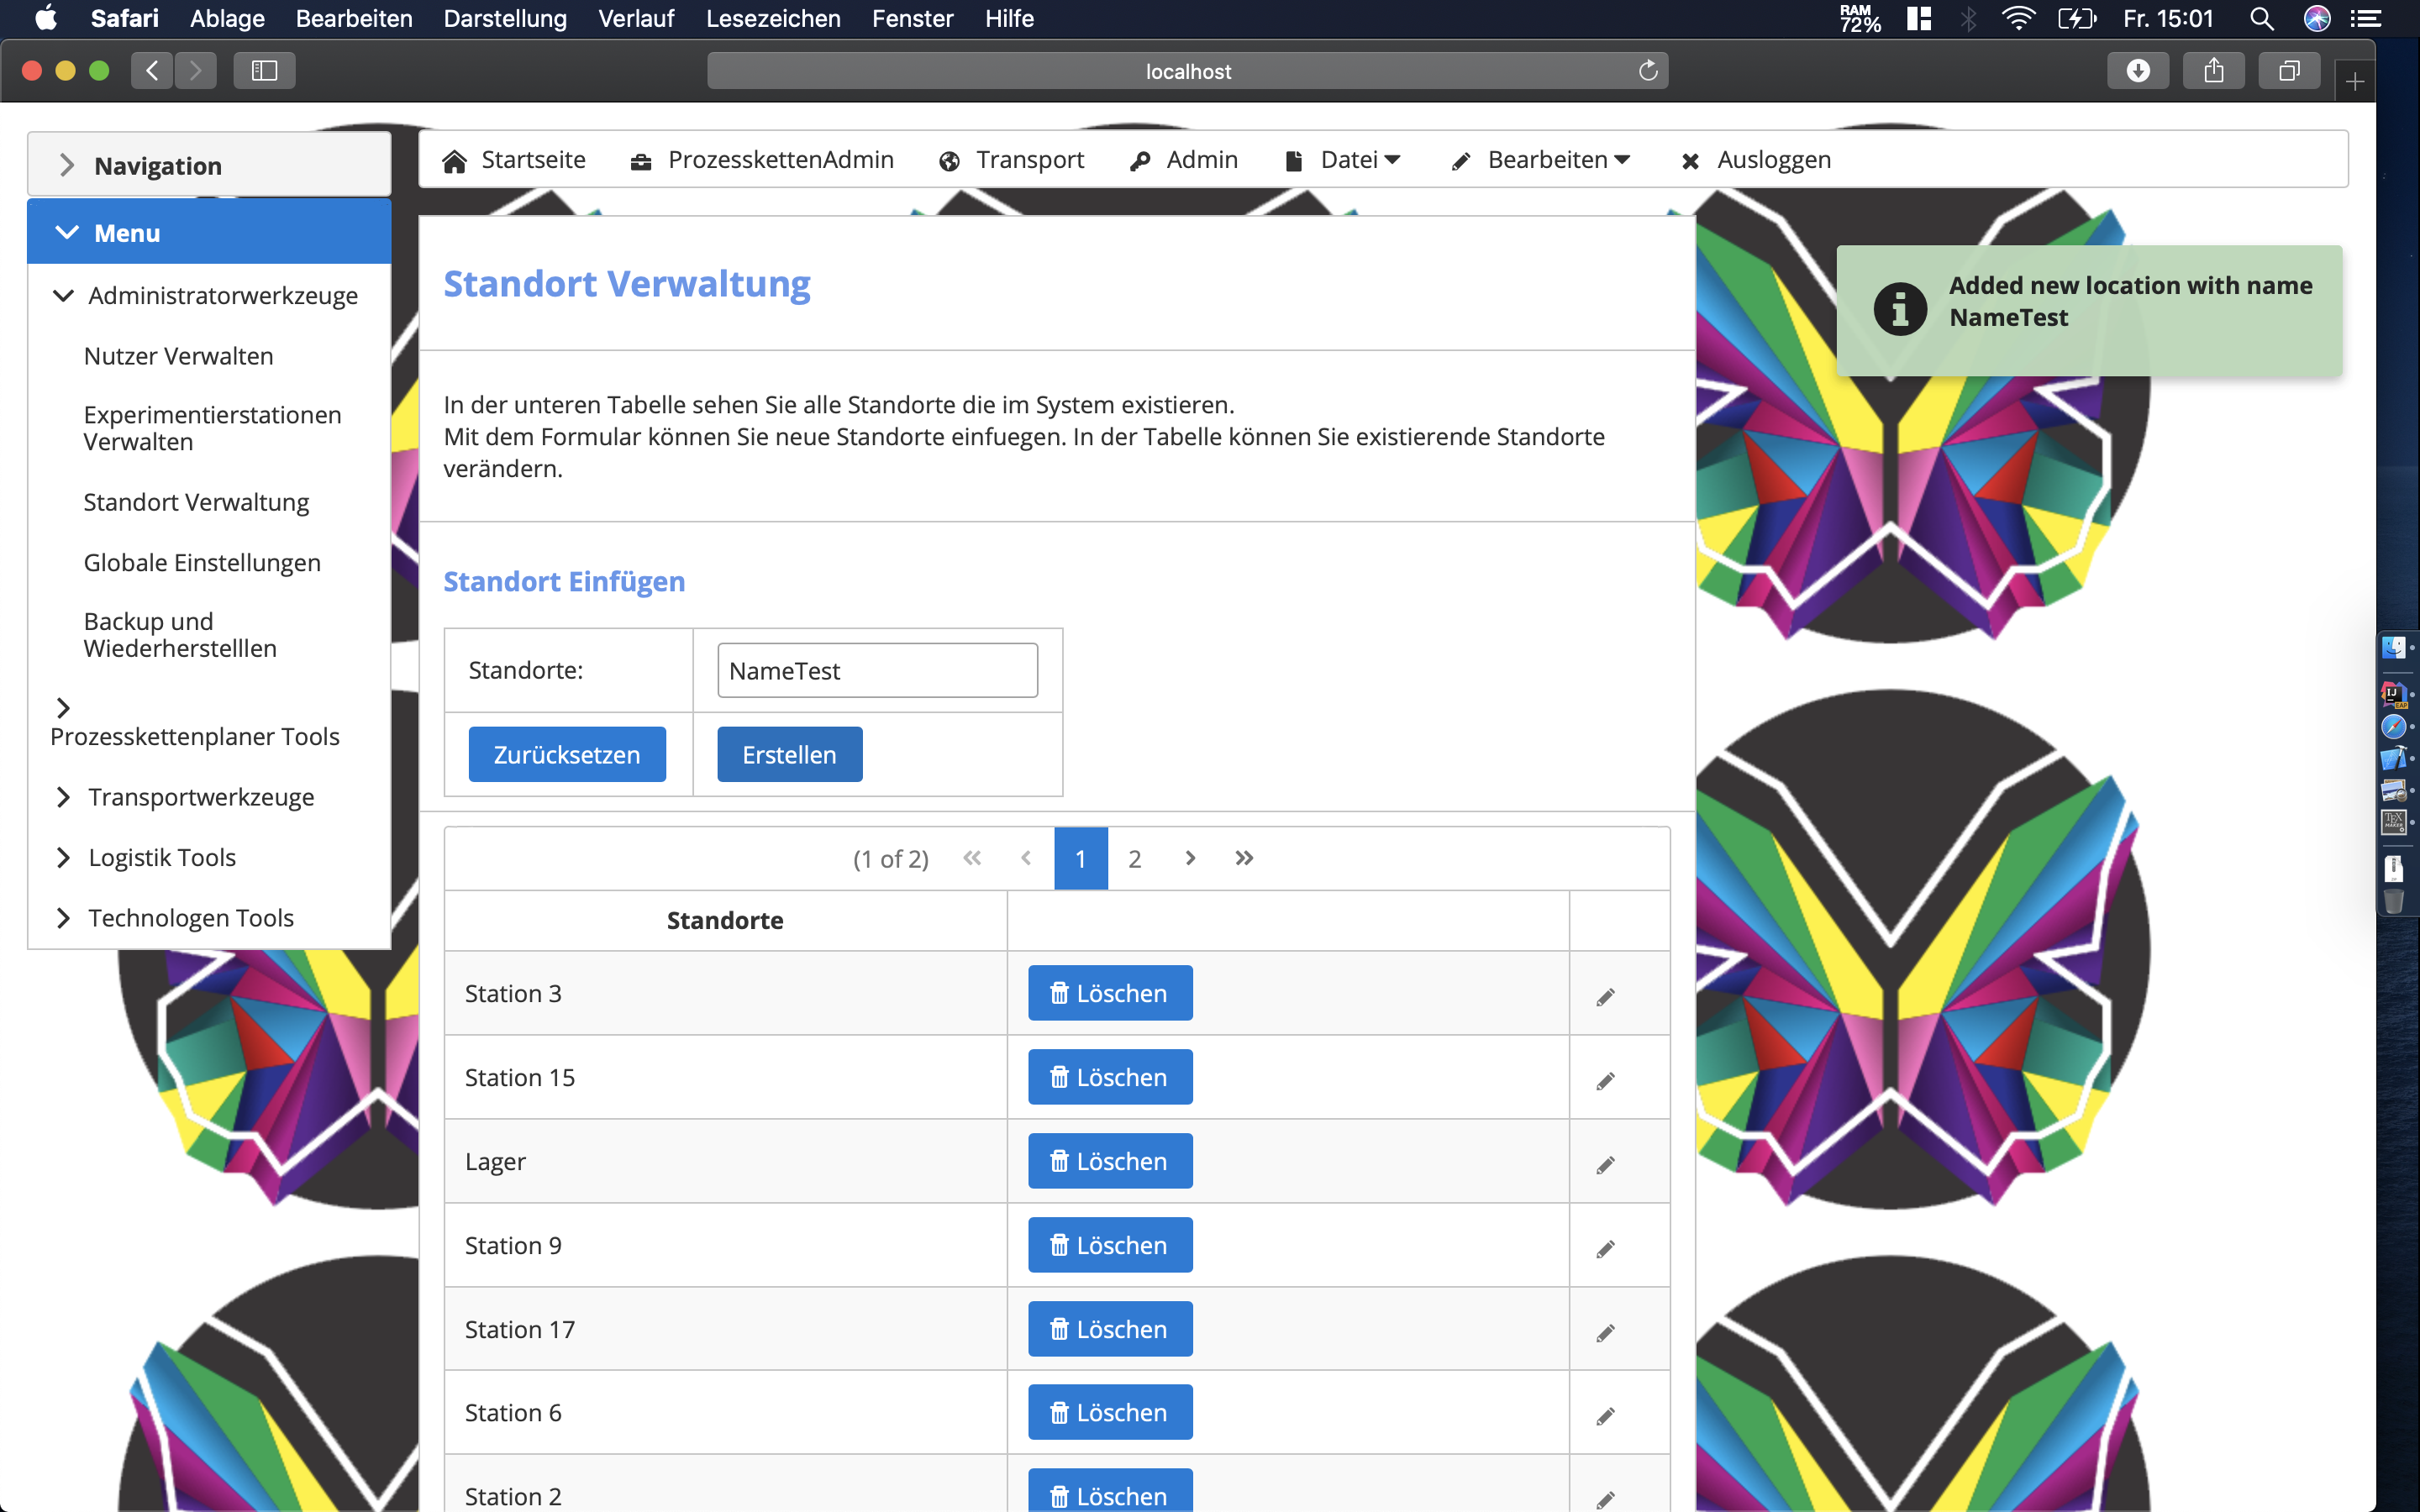
\includegraphics[width=1\textwidth]{Screenshots/4BeschaenigungAddLocation.png}
\textit{Abbildung 3.2.3.2: Standort Erzeugung}
} \\
Die erstellte Station befindet sich in der Tabelle.\\

\hypertarget{sc3.1.4.3}{
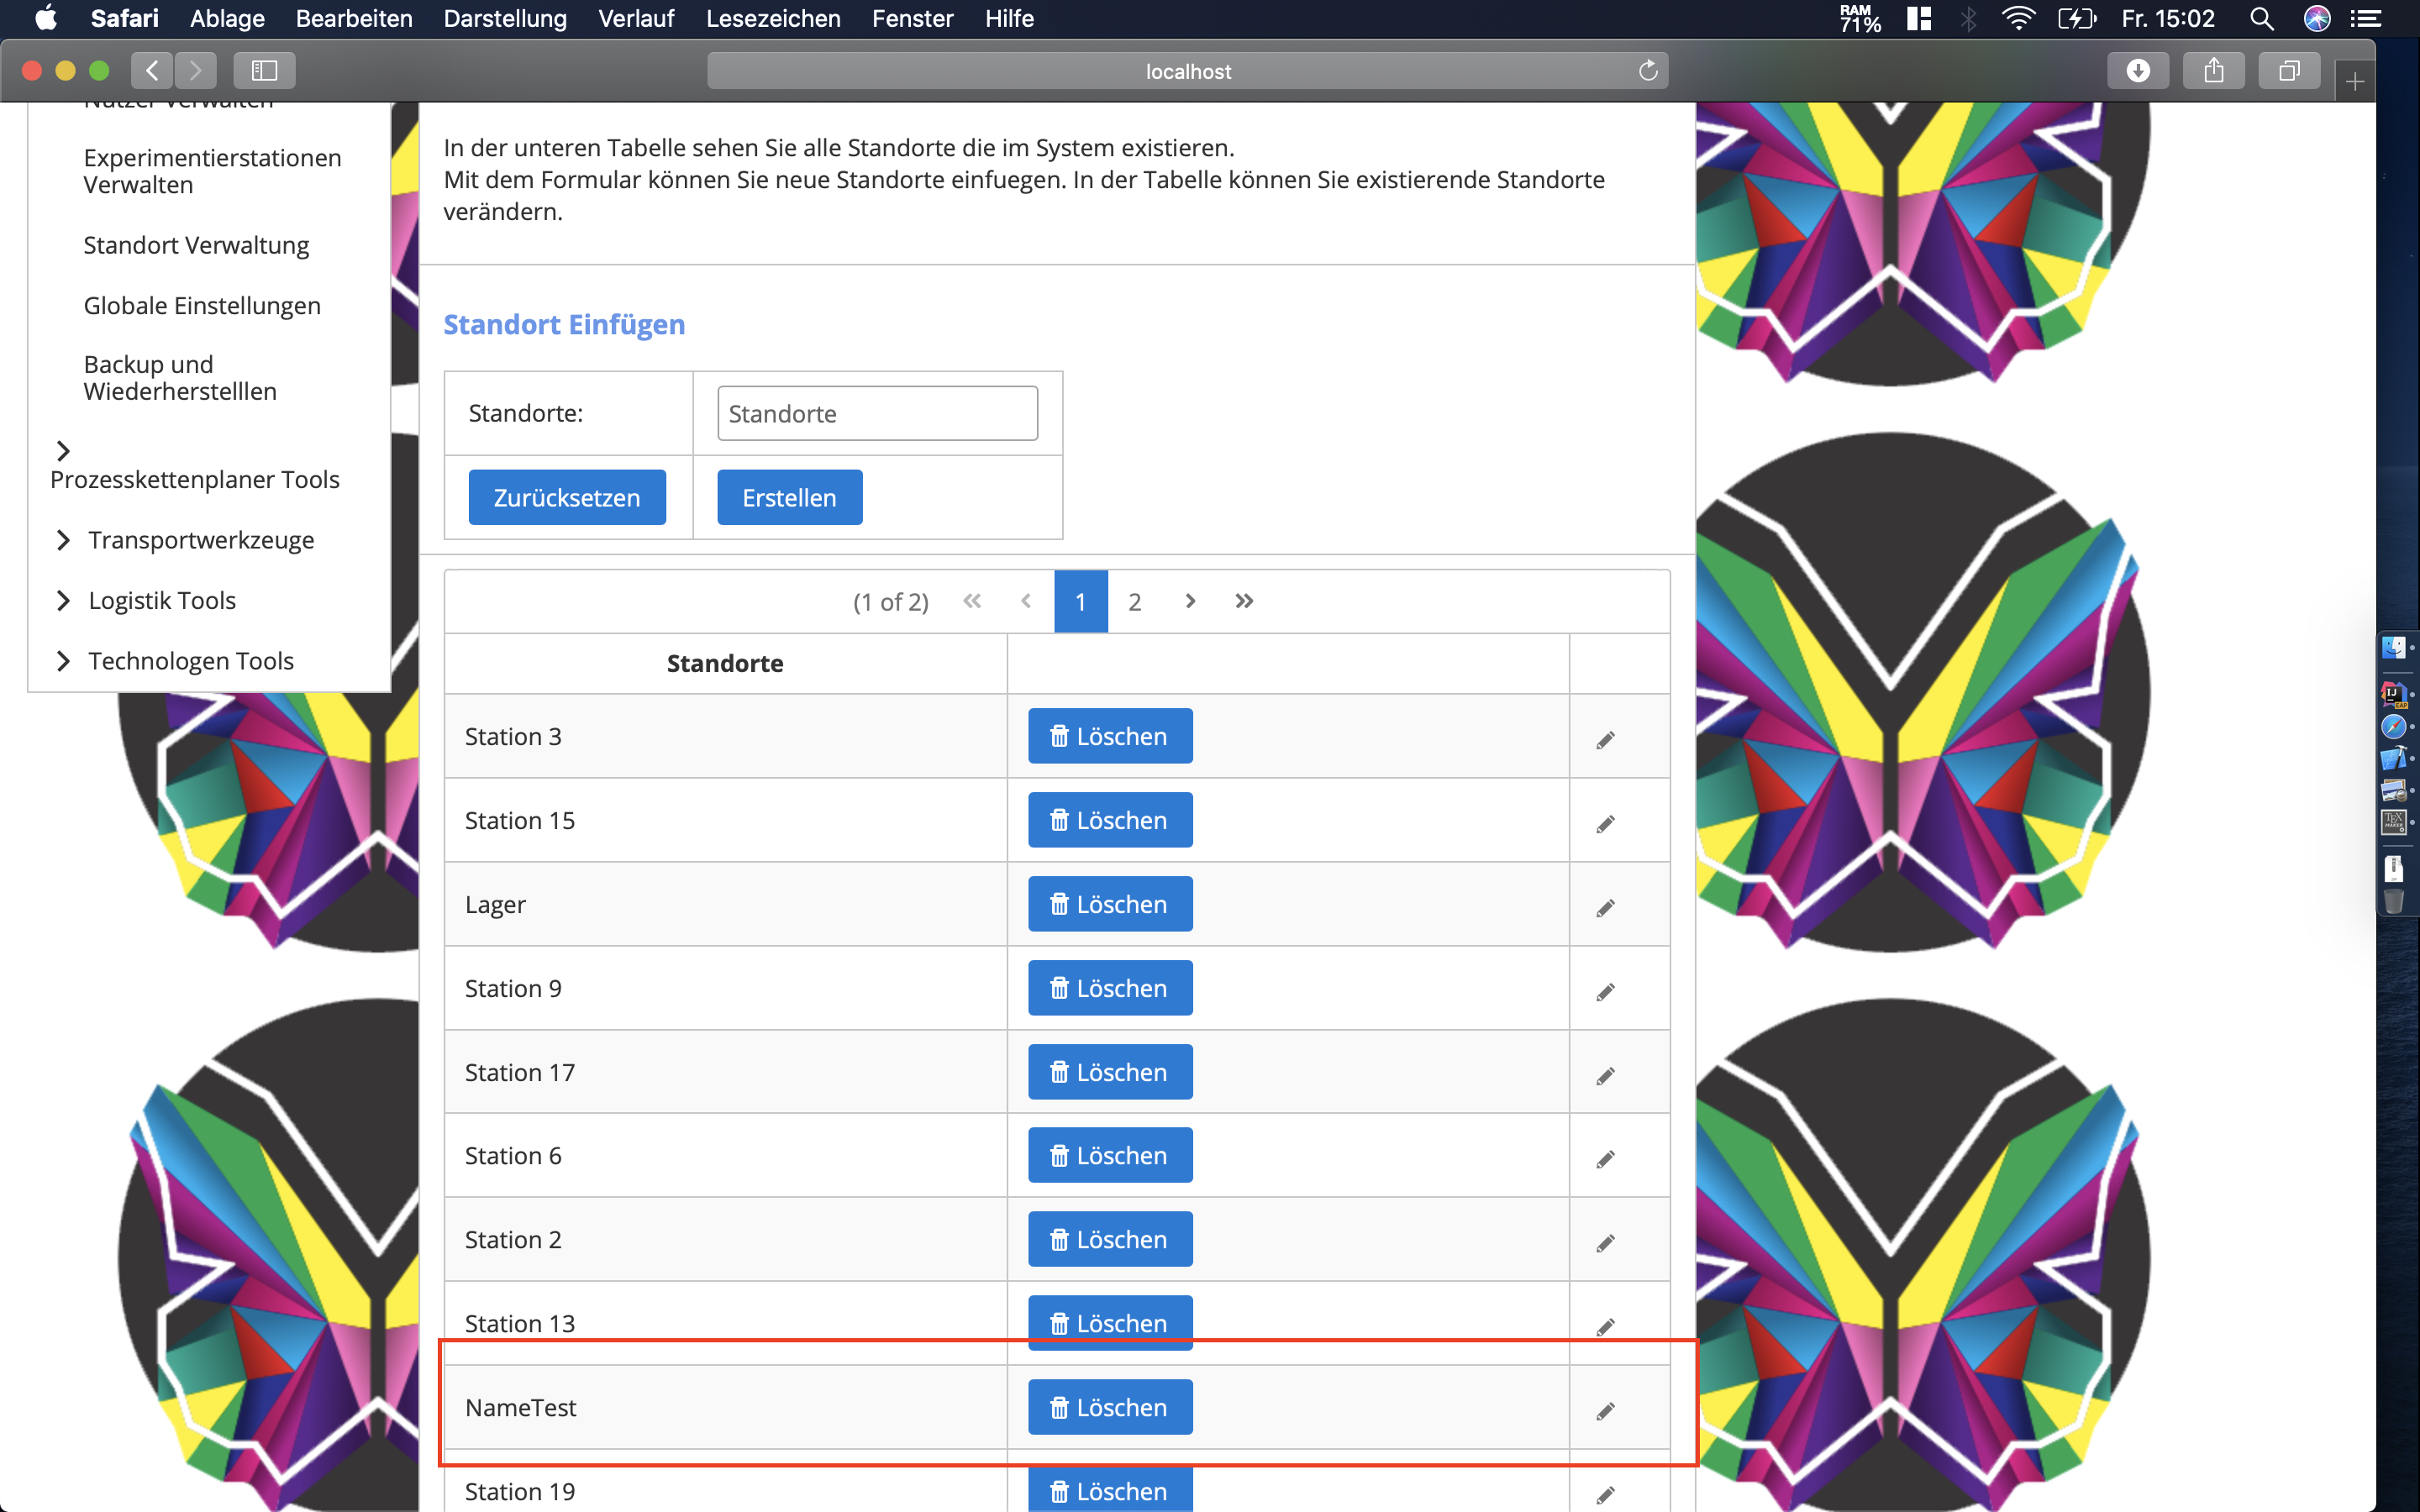
\includegraphics[width=1\textwidth]{Screenshots/4TestExperimentierteEstacion.png}
\textit{Abbildung 3.2.3.3: Standort an der Tabelle}
} \\
Wenn eine Station erstellt wird, wird eine Bestätigungsnachricht durch der Website empfangen.\\

\hypertarget{sc3.1.4.4}{
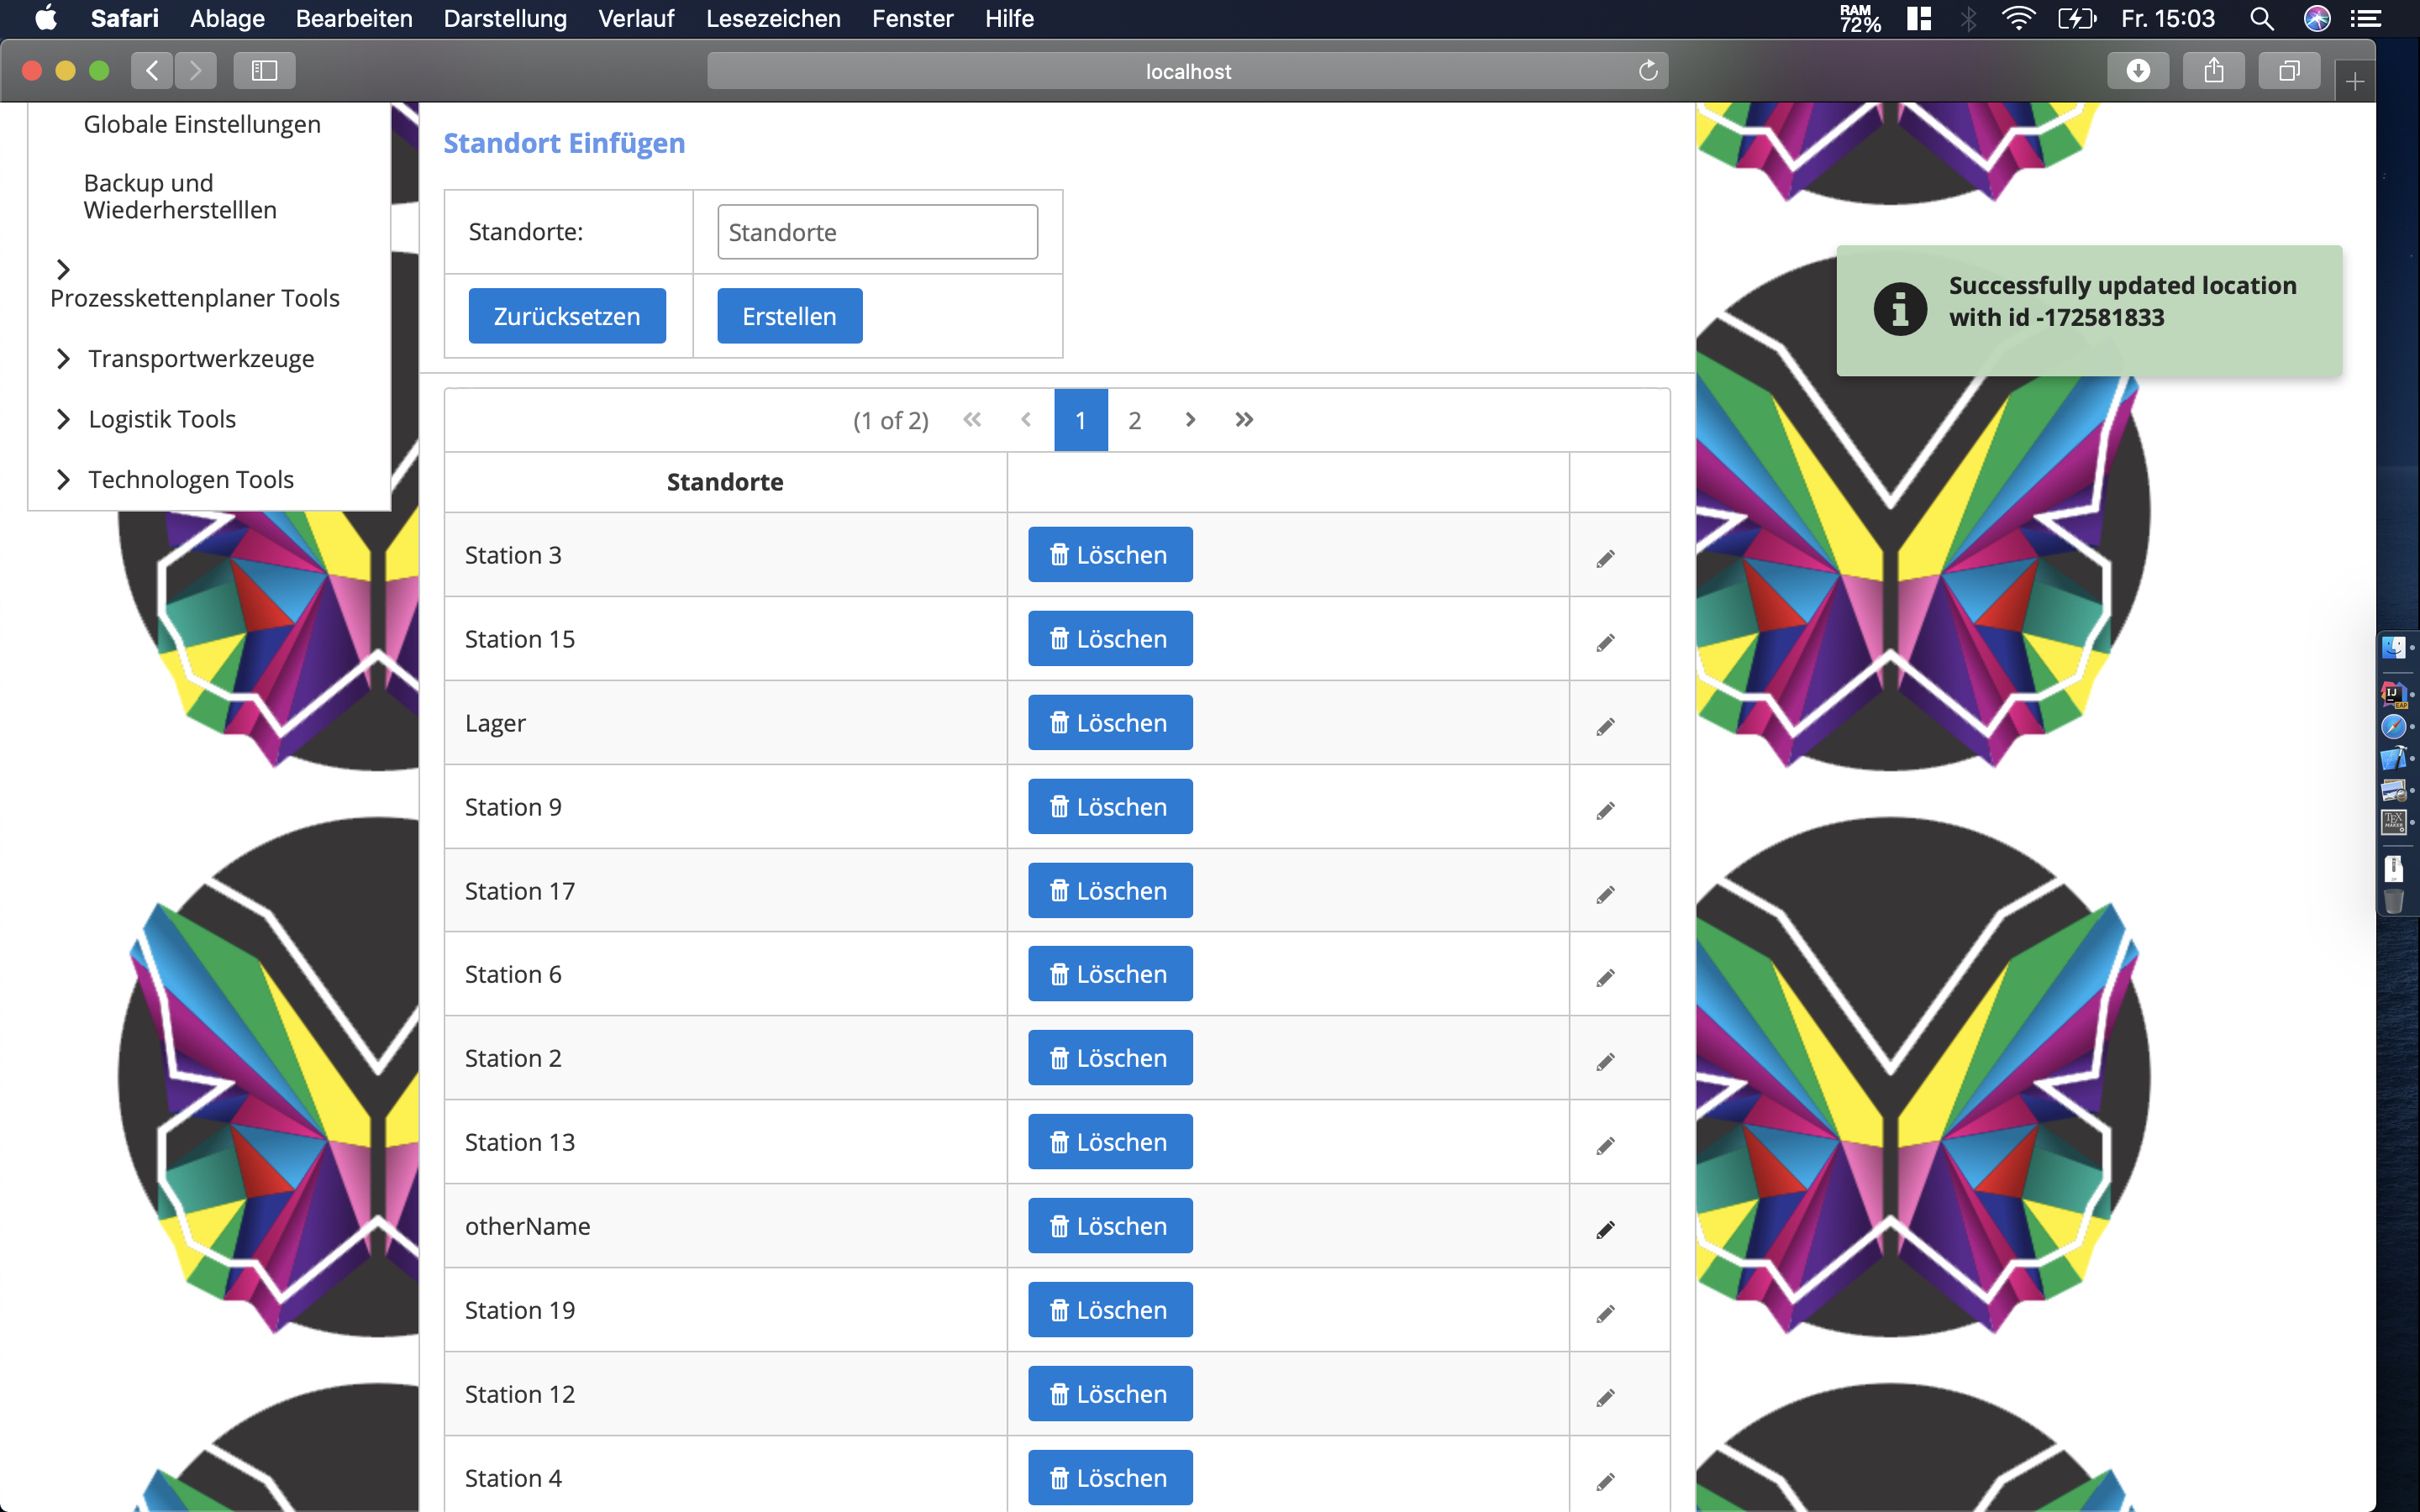
\includegraphics[width=1\textwidth]{Screenshots/4UpdateStantion.png}
\textit{Abbildung 3.2.3.4:  Standort Editieren}
} \\
Auf die gleiche Weise wird beim Drücken der Löschtaste eine Bestätigungsnachricht über die Tabelle der Webseite empfangen.\\

\hypertarget{sc3.1.4.5}{
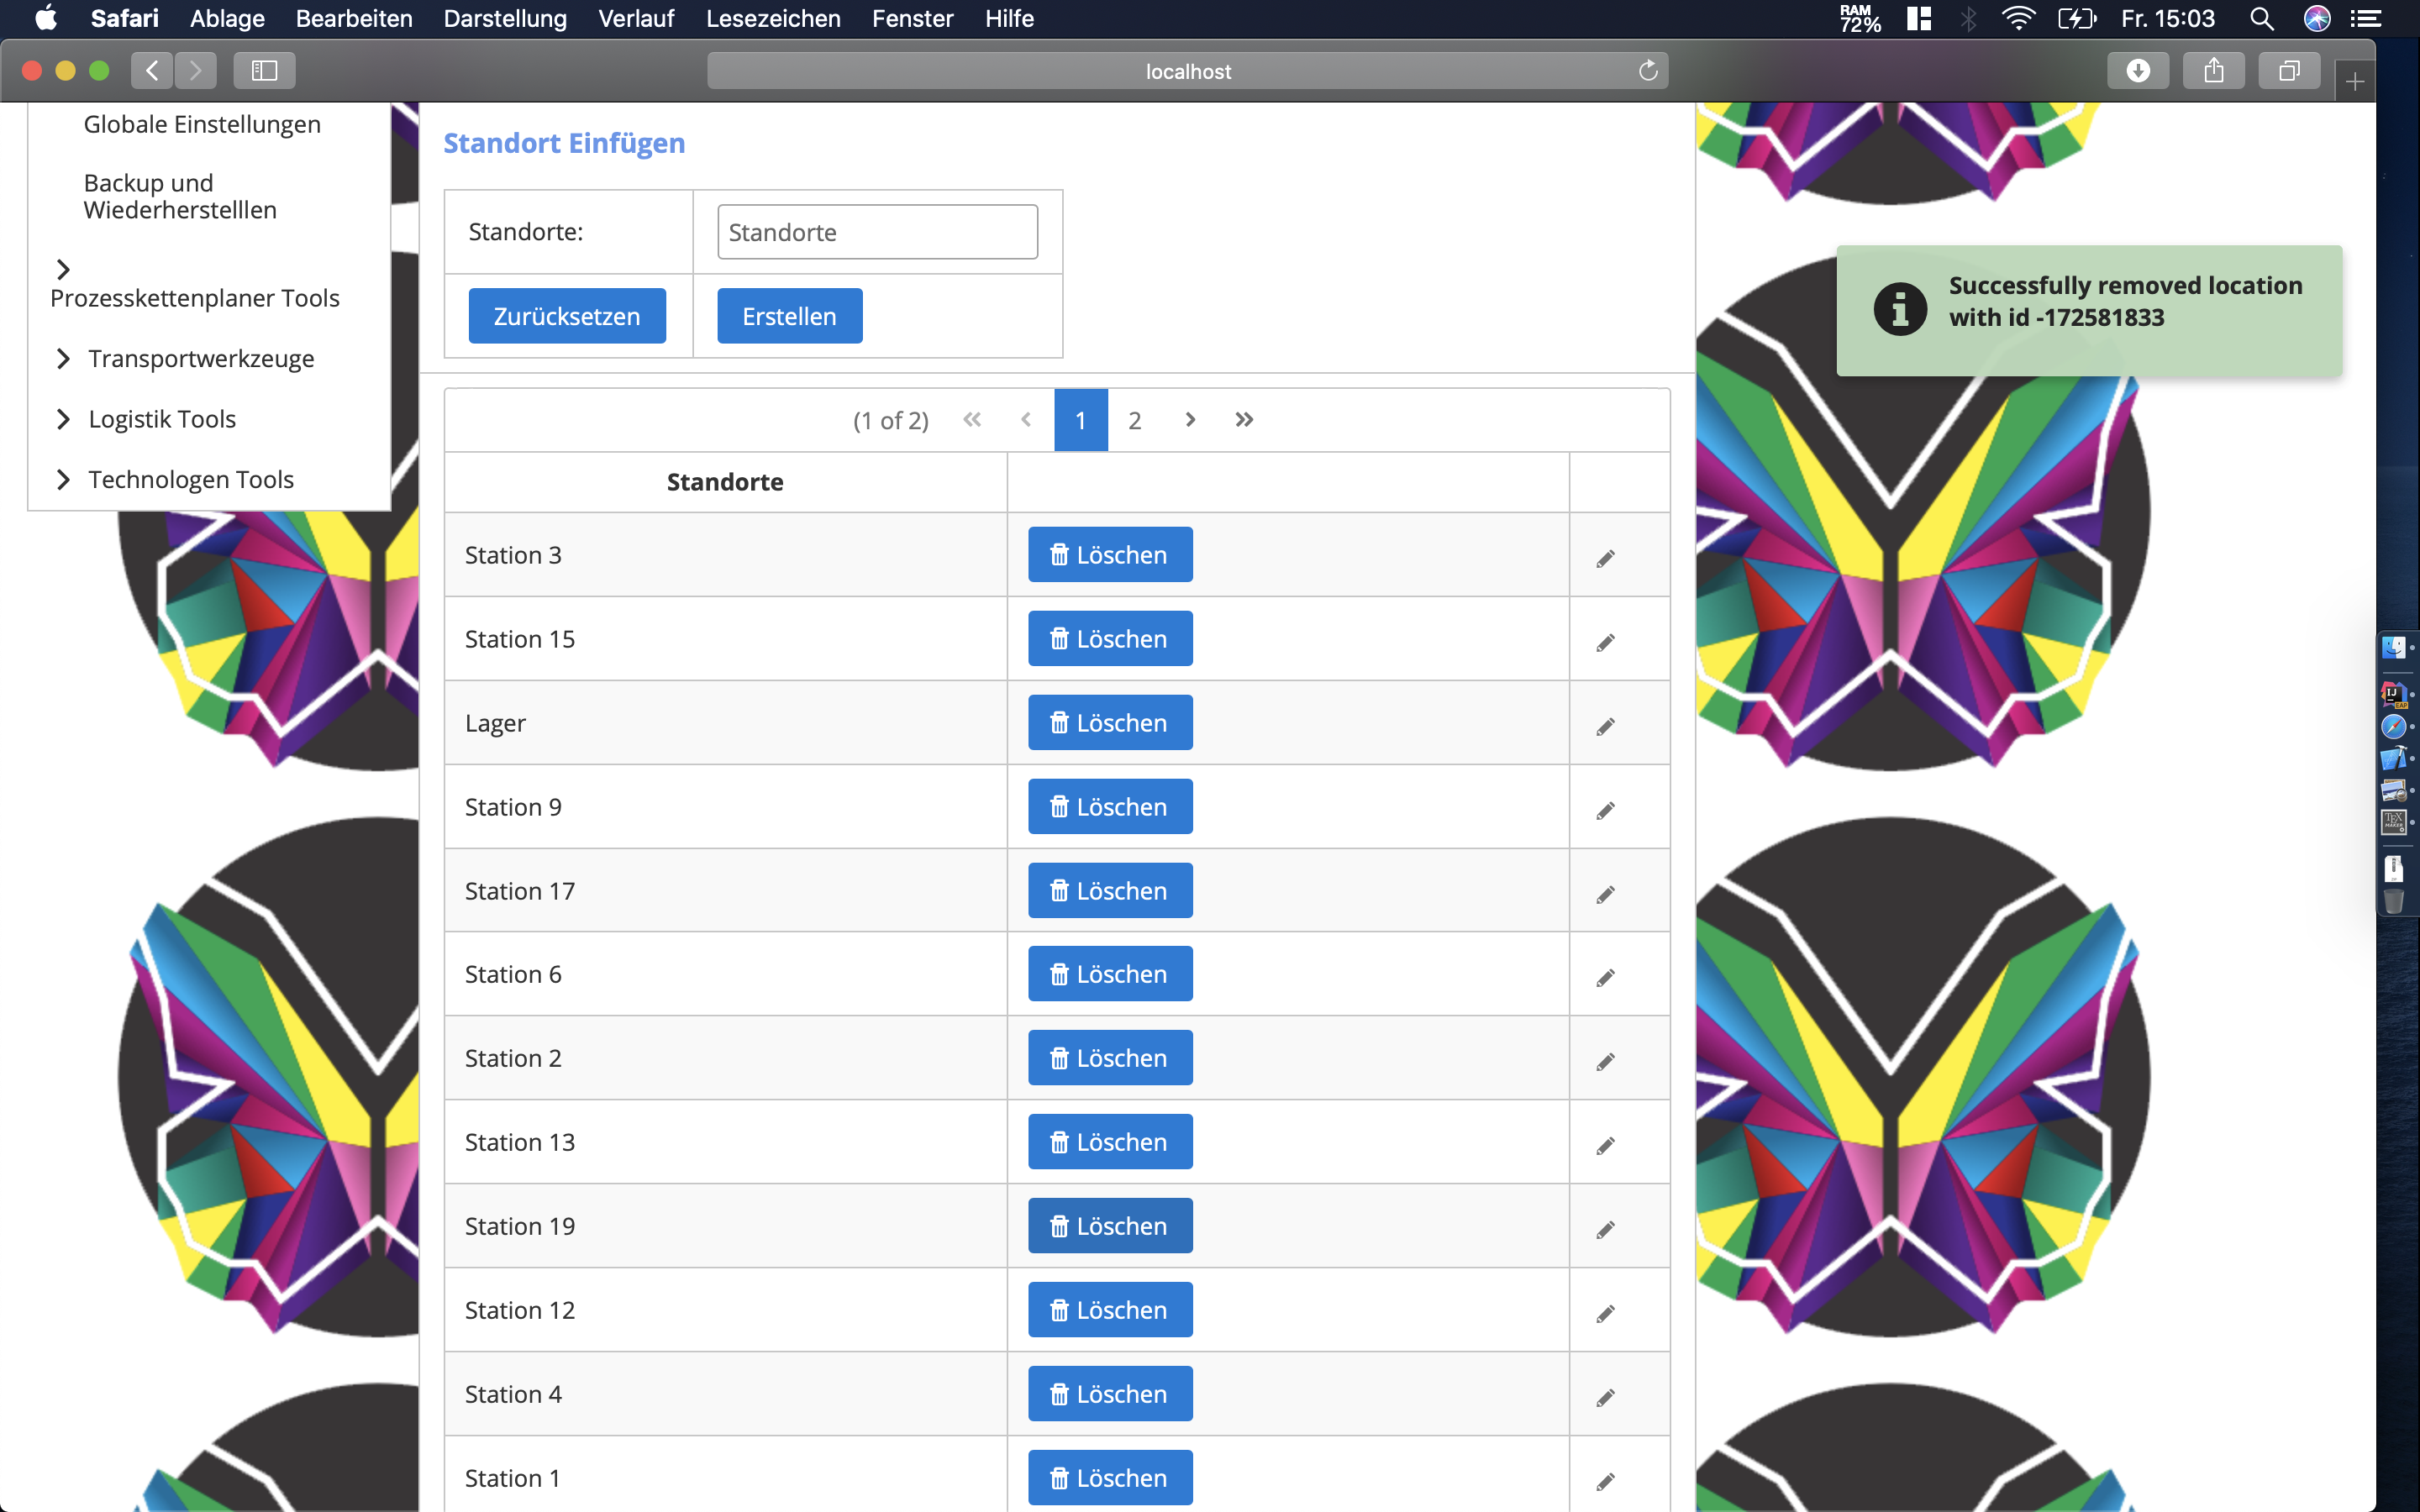
\includegraphics[width=1\textwidth]{Screenshots/4RemoveStation.png}
\textit{Abbildung 3.2.3.5: Standort Entfernen}
} \\
%%

\subsubsection{Anwendungsfall: Backup}


Um ein Backup der Datenbank zu speichern, muss der Administrator auf der entsprechenden Website auf die knoten Sichern klicken.\\
\hypertarget{sc3.1.5.1}{
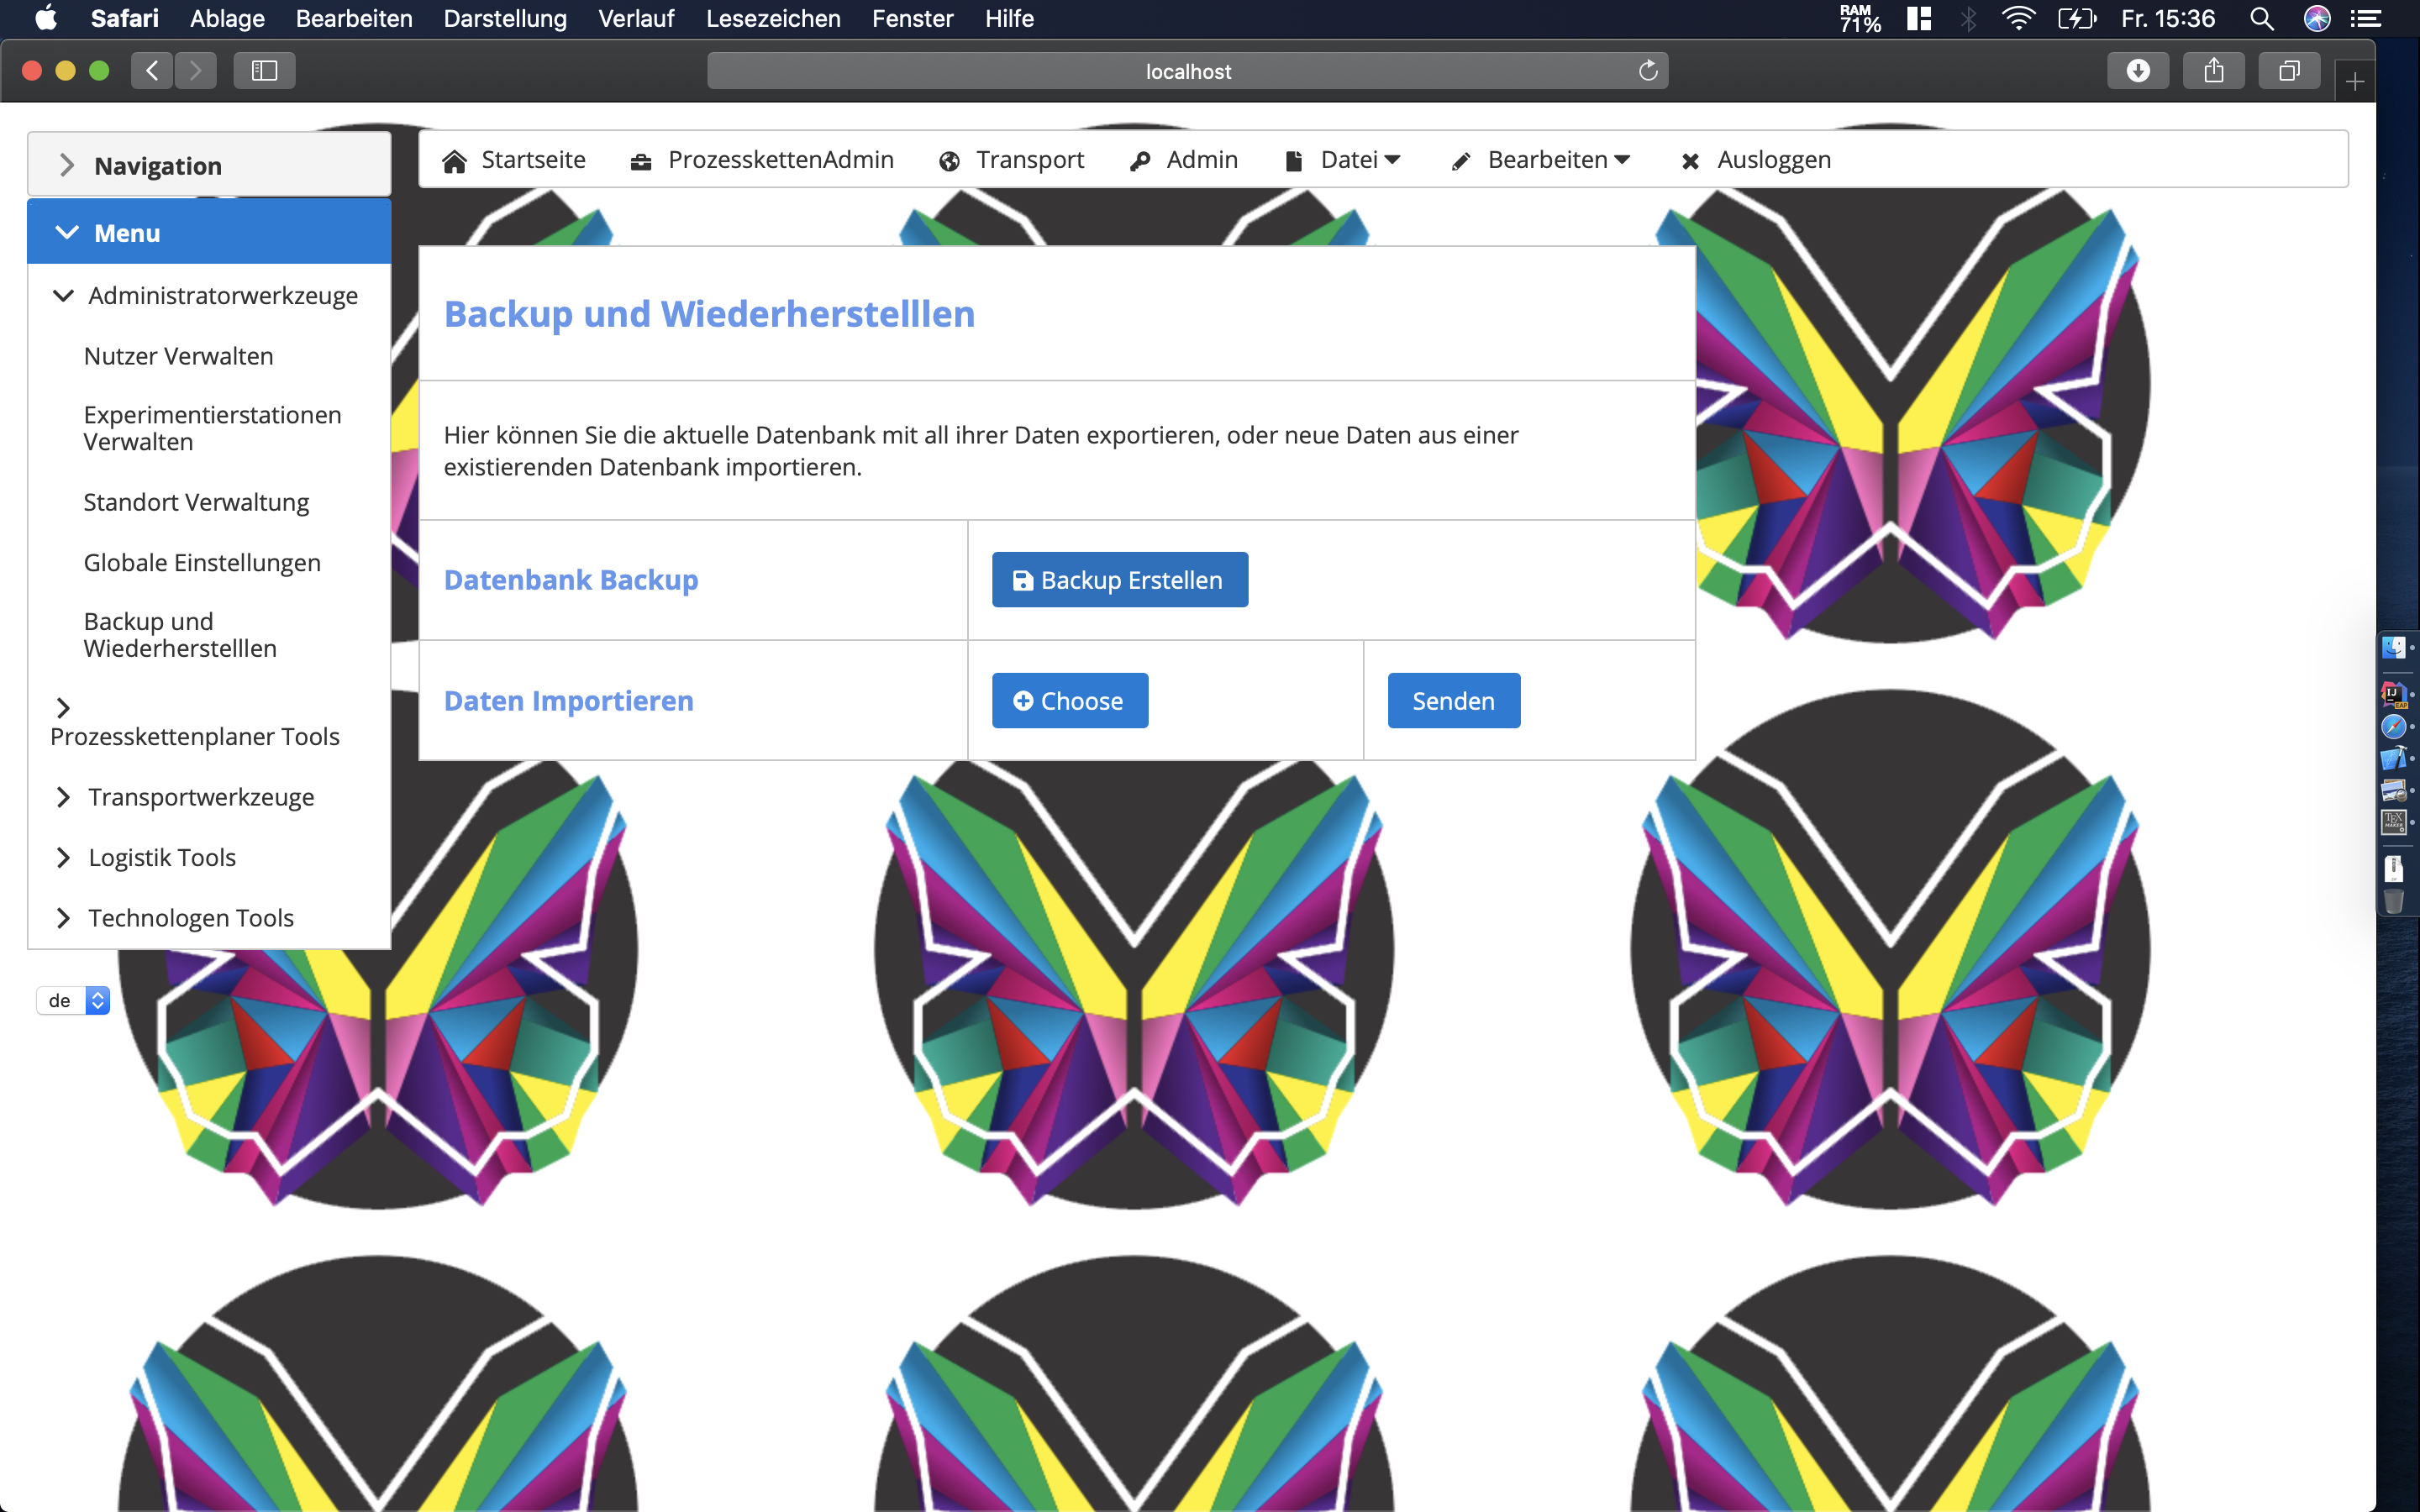
\includegraphics[width=1\textwidth]{Screenshots/5BackFormular.png}
\textit{Abbildung 3.2.4.1: Standort Formular}
} \\

Wenn das Backup generiert wird, sendet die Webseite eine Bestätigungsnachricht.\\
\hypertarget{sc3.1.5.2}{
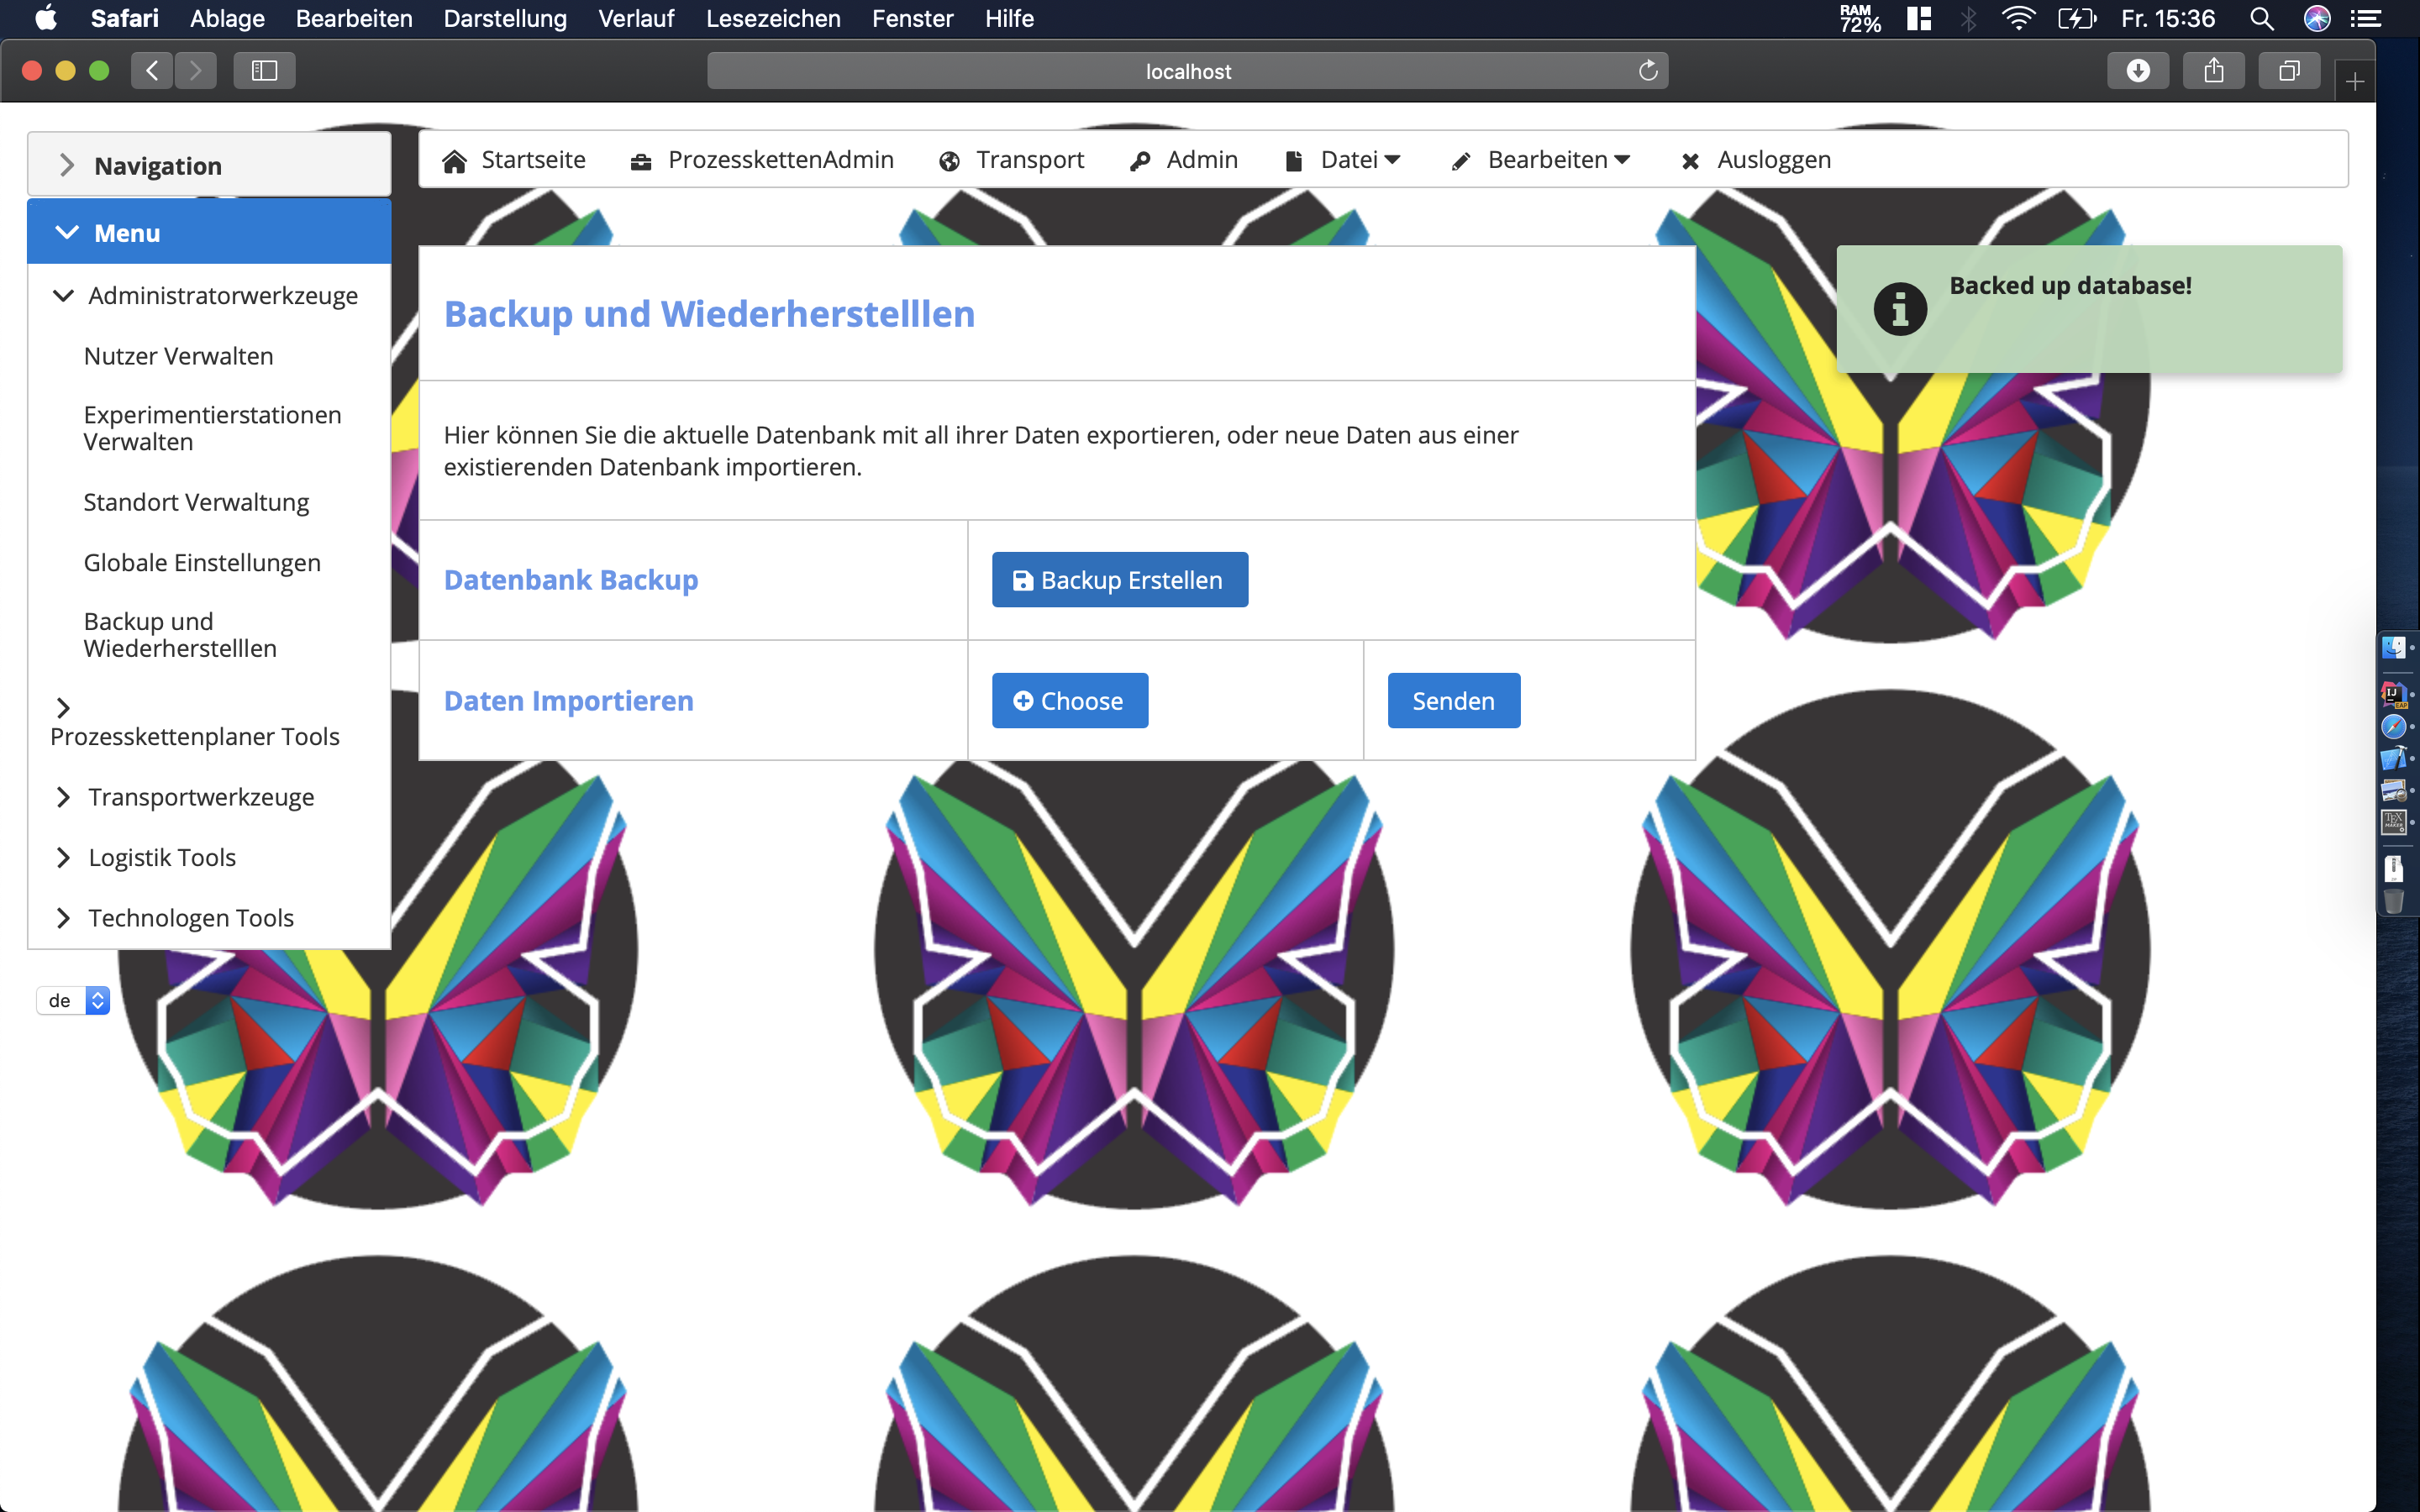
\includegraphics[width=1\textwidth]{Screenshots/5BackGenerated.png}
\textit{Abbildung 3.2.4.2: Standort Formular}
} \\

Die Generierung der Datei wurde getestet.\\

\hypertarget{sc3.1.5.3}{
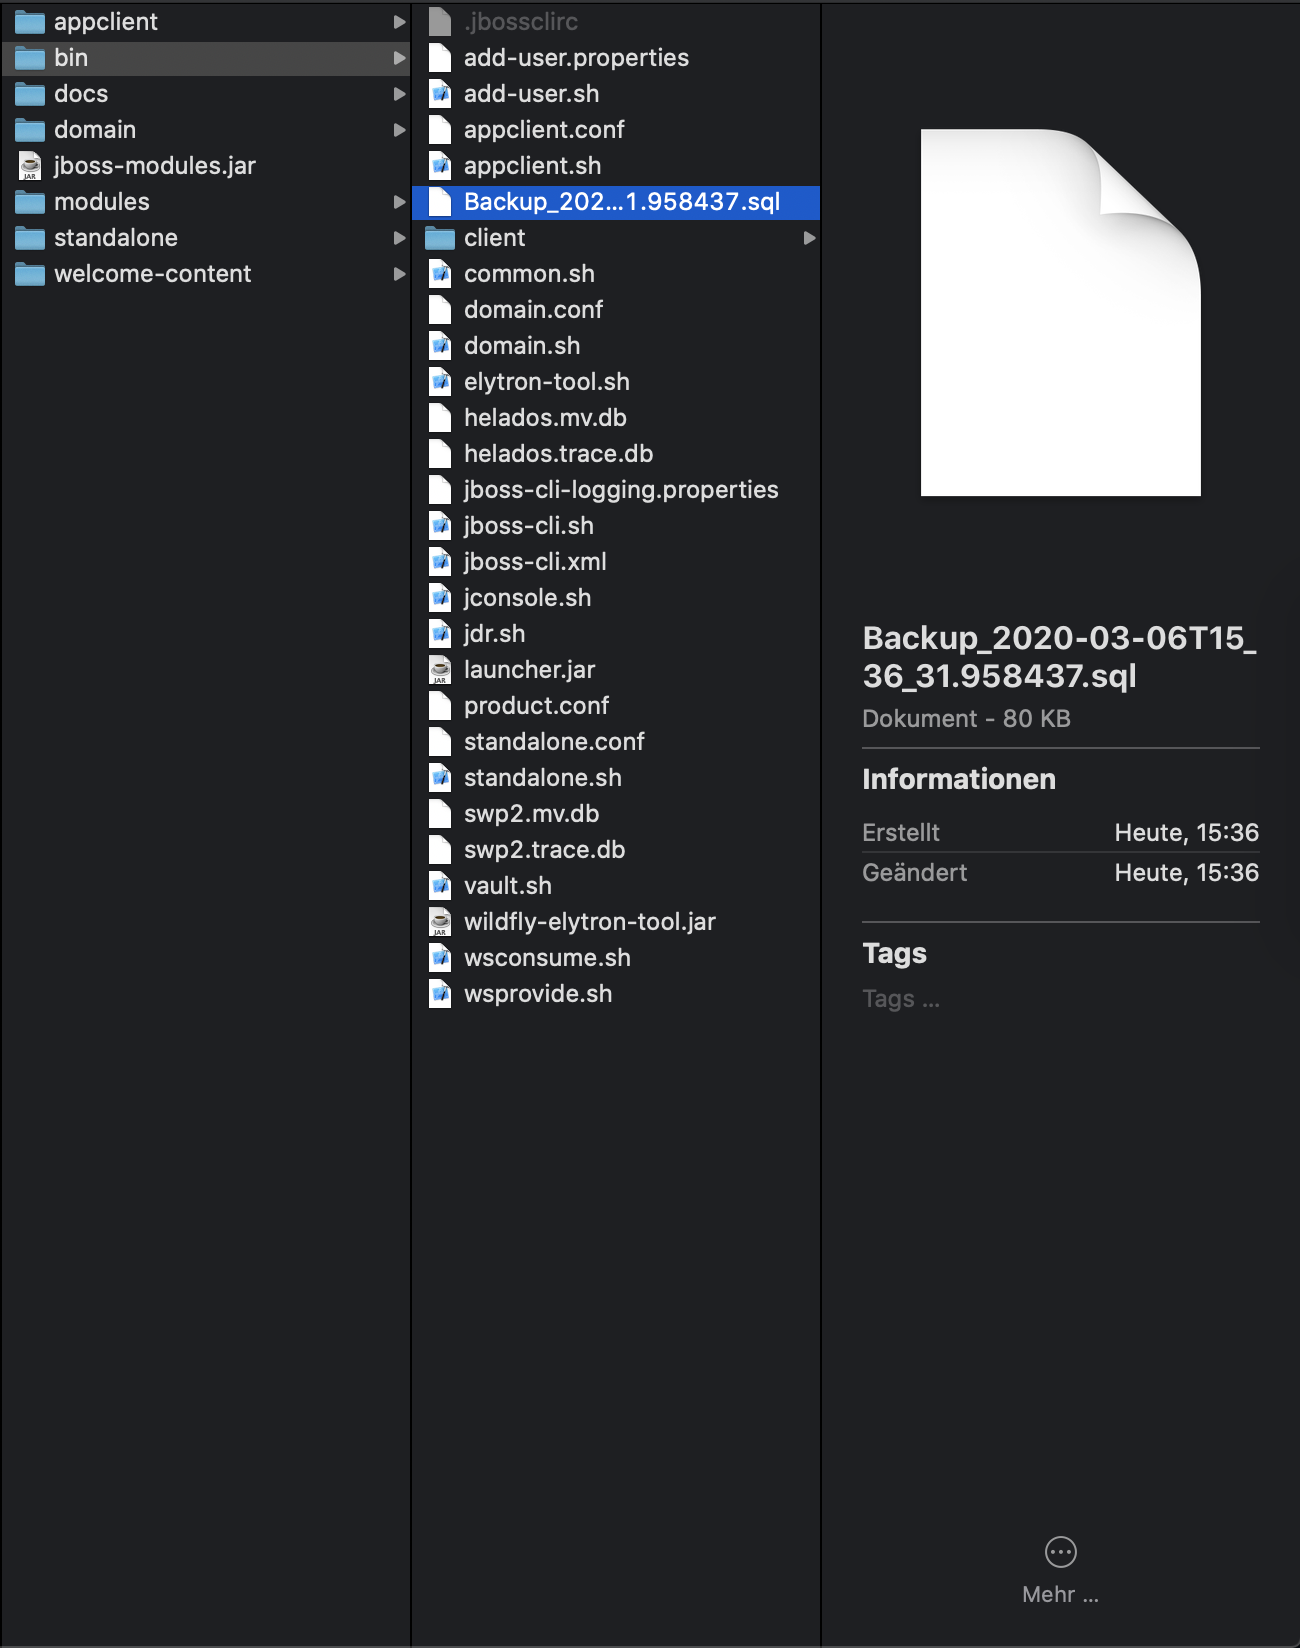
\includegraphics[width=1\textwidth]{Screenshots/5BackUpDatei.png}
\textit{Abbildung 3.2.4.3: Standort Formular}
} \\
Um den Import der Datenbanken zu testen, wurden alle Systembenutzer entfernt. Sobald eine Datendatei mit neuen Benutzern importiert wurde.\\
\hypertarget{sc3.1.5.4}{
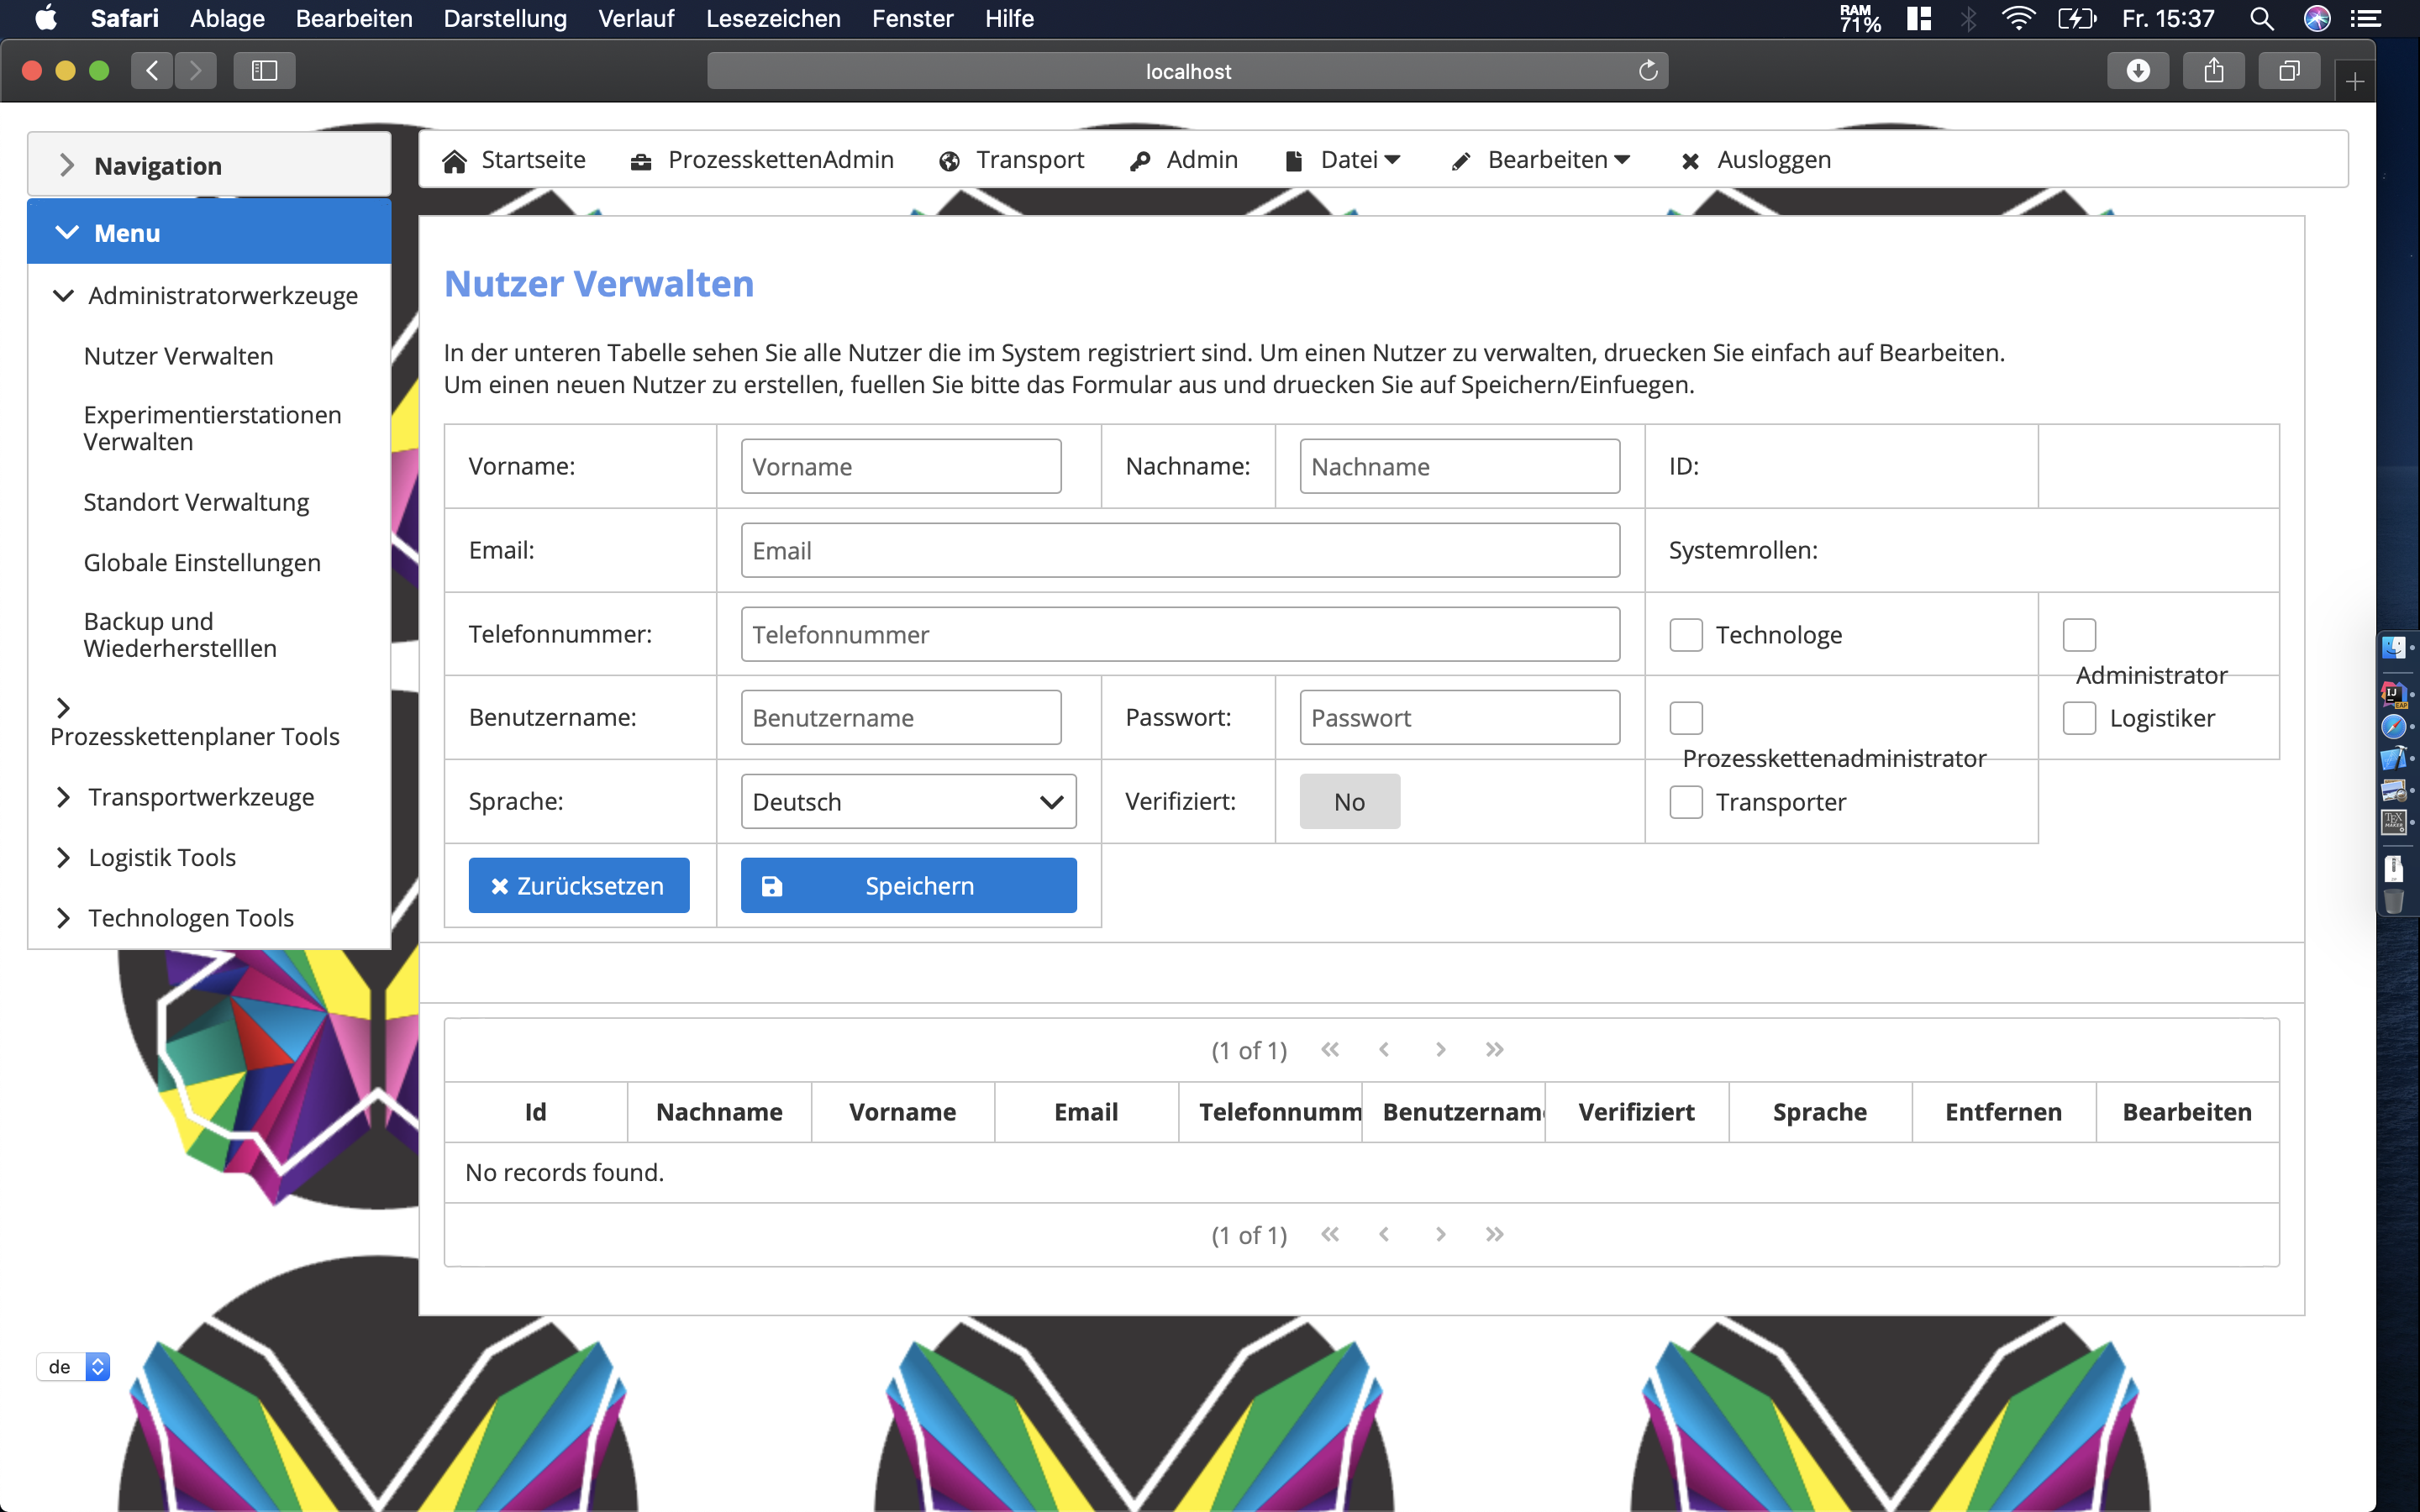
\includegraphics[width=1\textwidth]{Screenshots/5NotUsers.png}
\textit{Abbildung 3.2.4.4: Standort Formular}
} \\

\hypertarget{sc3.1.5.5}{
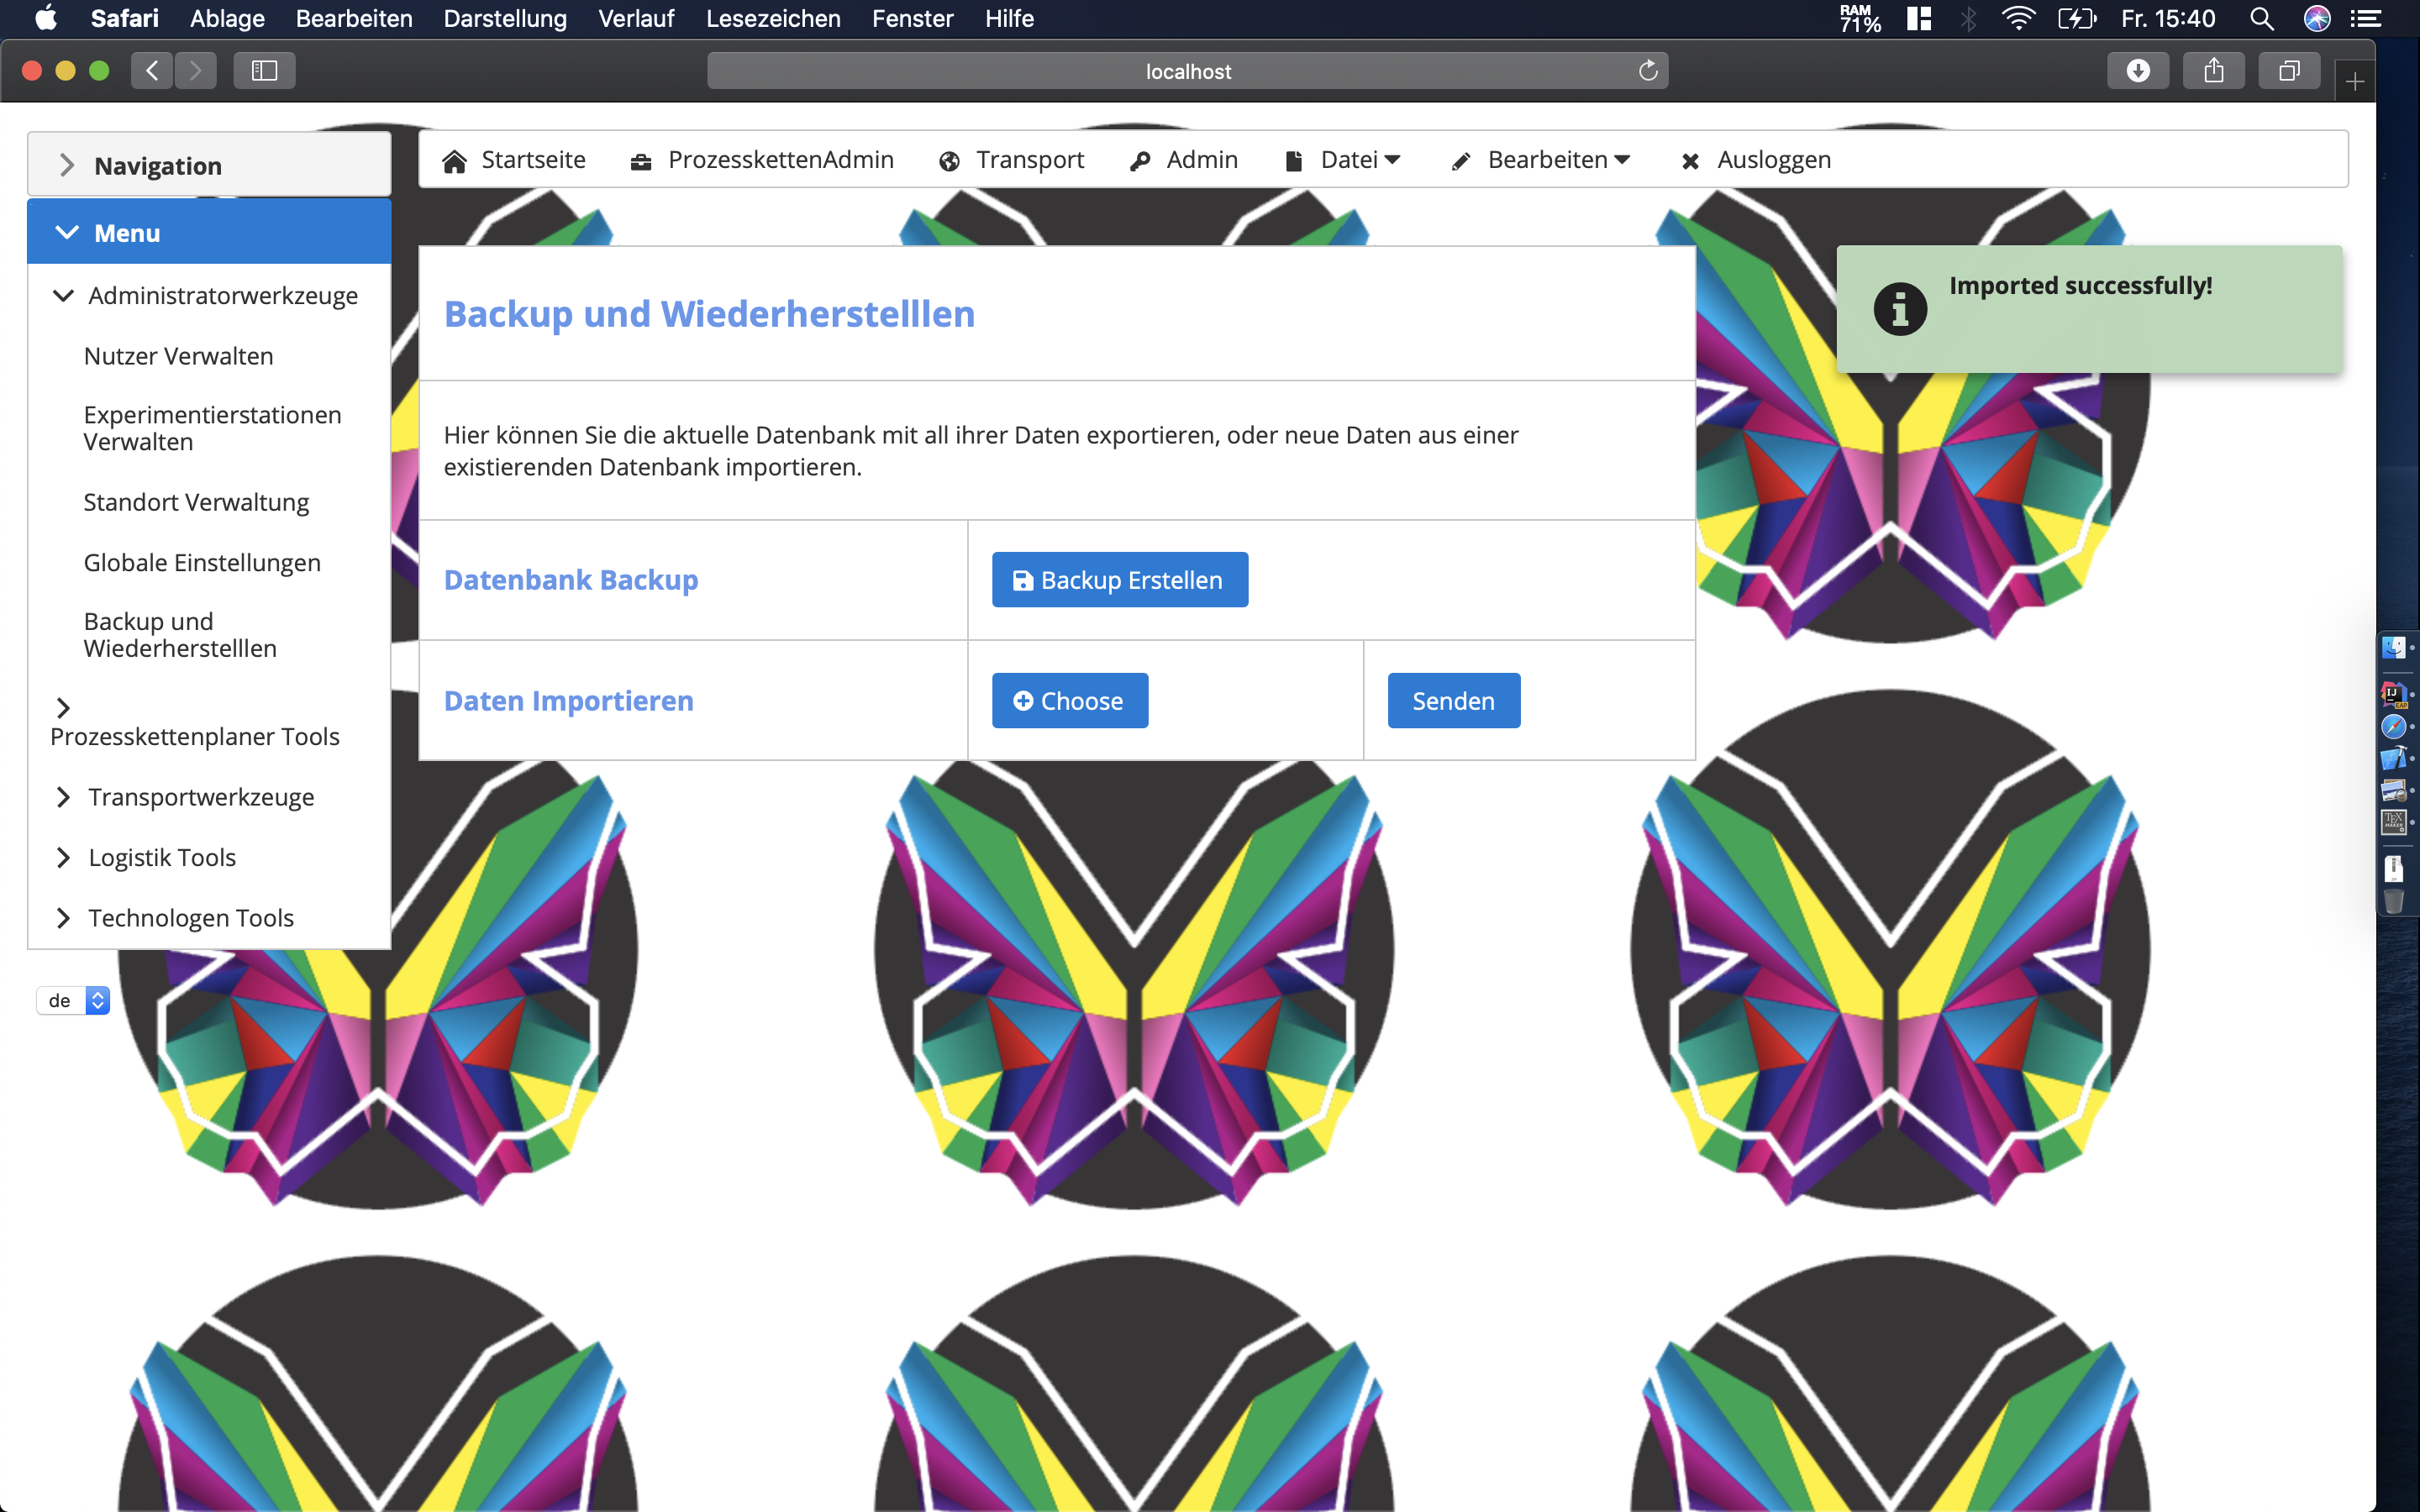
\includegraphics[width=1\textwidth]{Screenshots/5BackImported.png}
\textit{Abbildung 3.2.4.5: Standort Formular}
} \\
In der folgenden Grafik sehen Sie, dass die Benutzer erfolgreich aktualisiert wurden.\\

\hypertarget{sc3.1.5.6}{
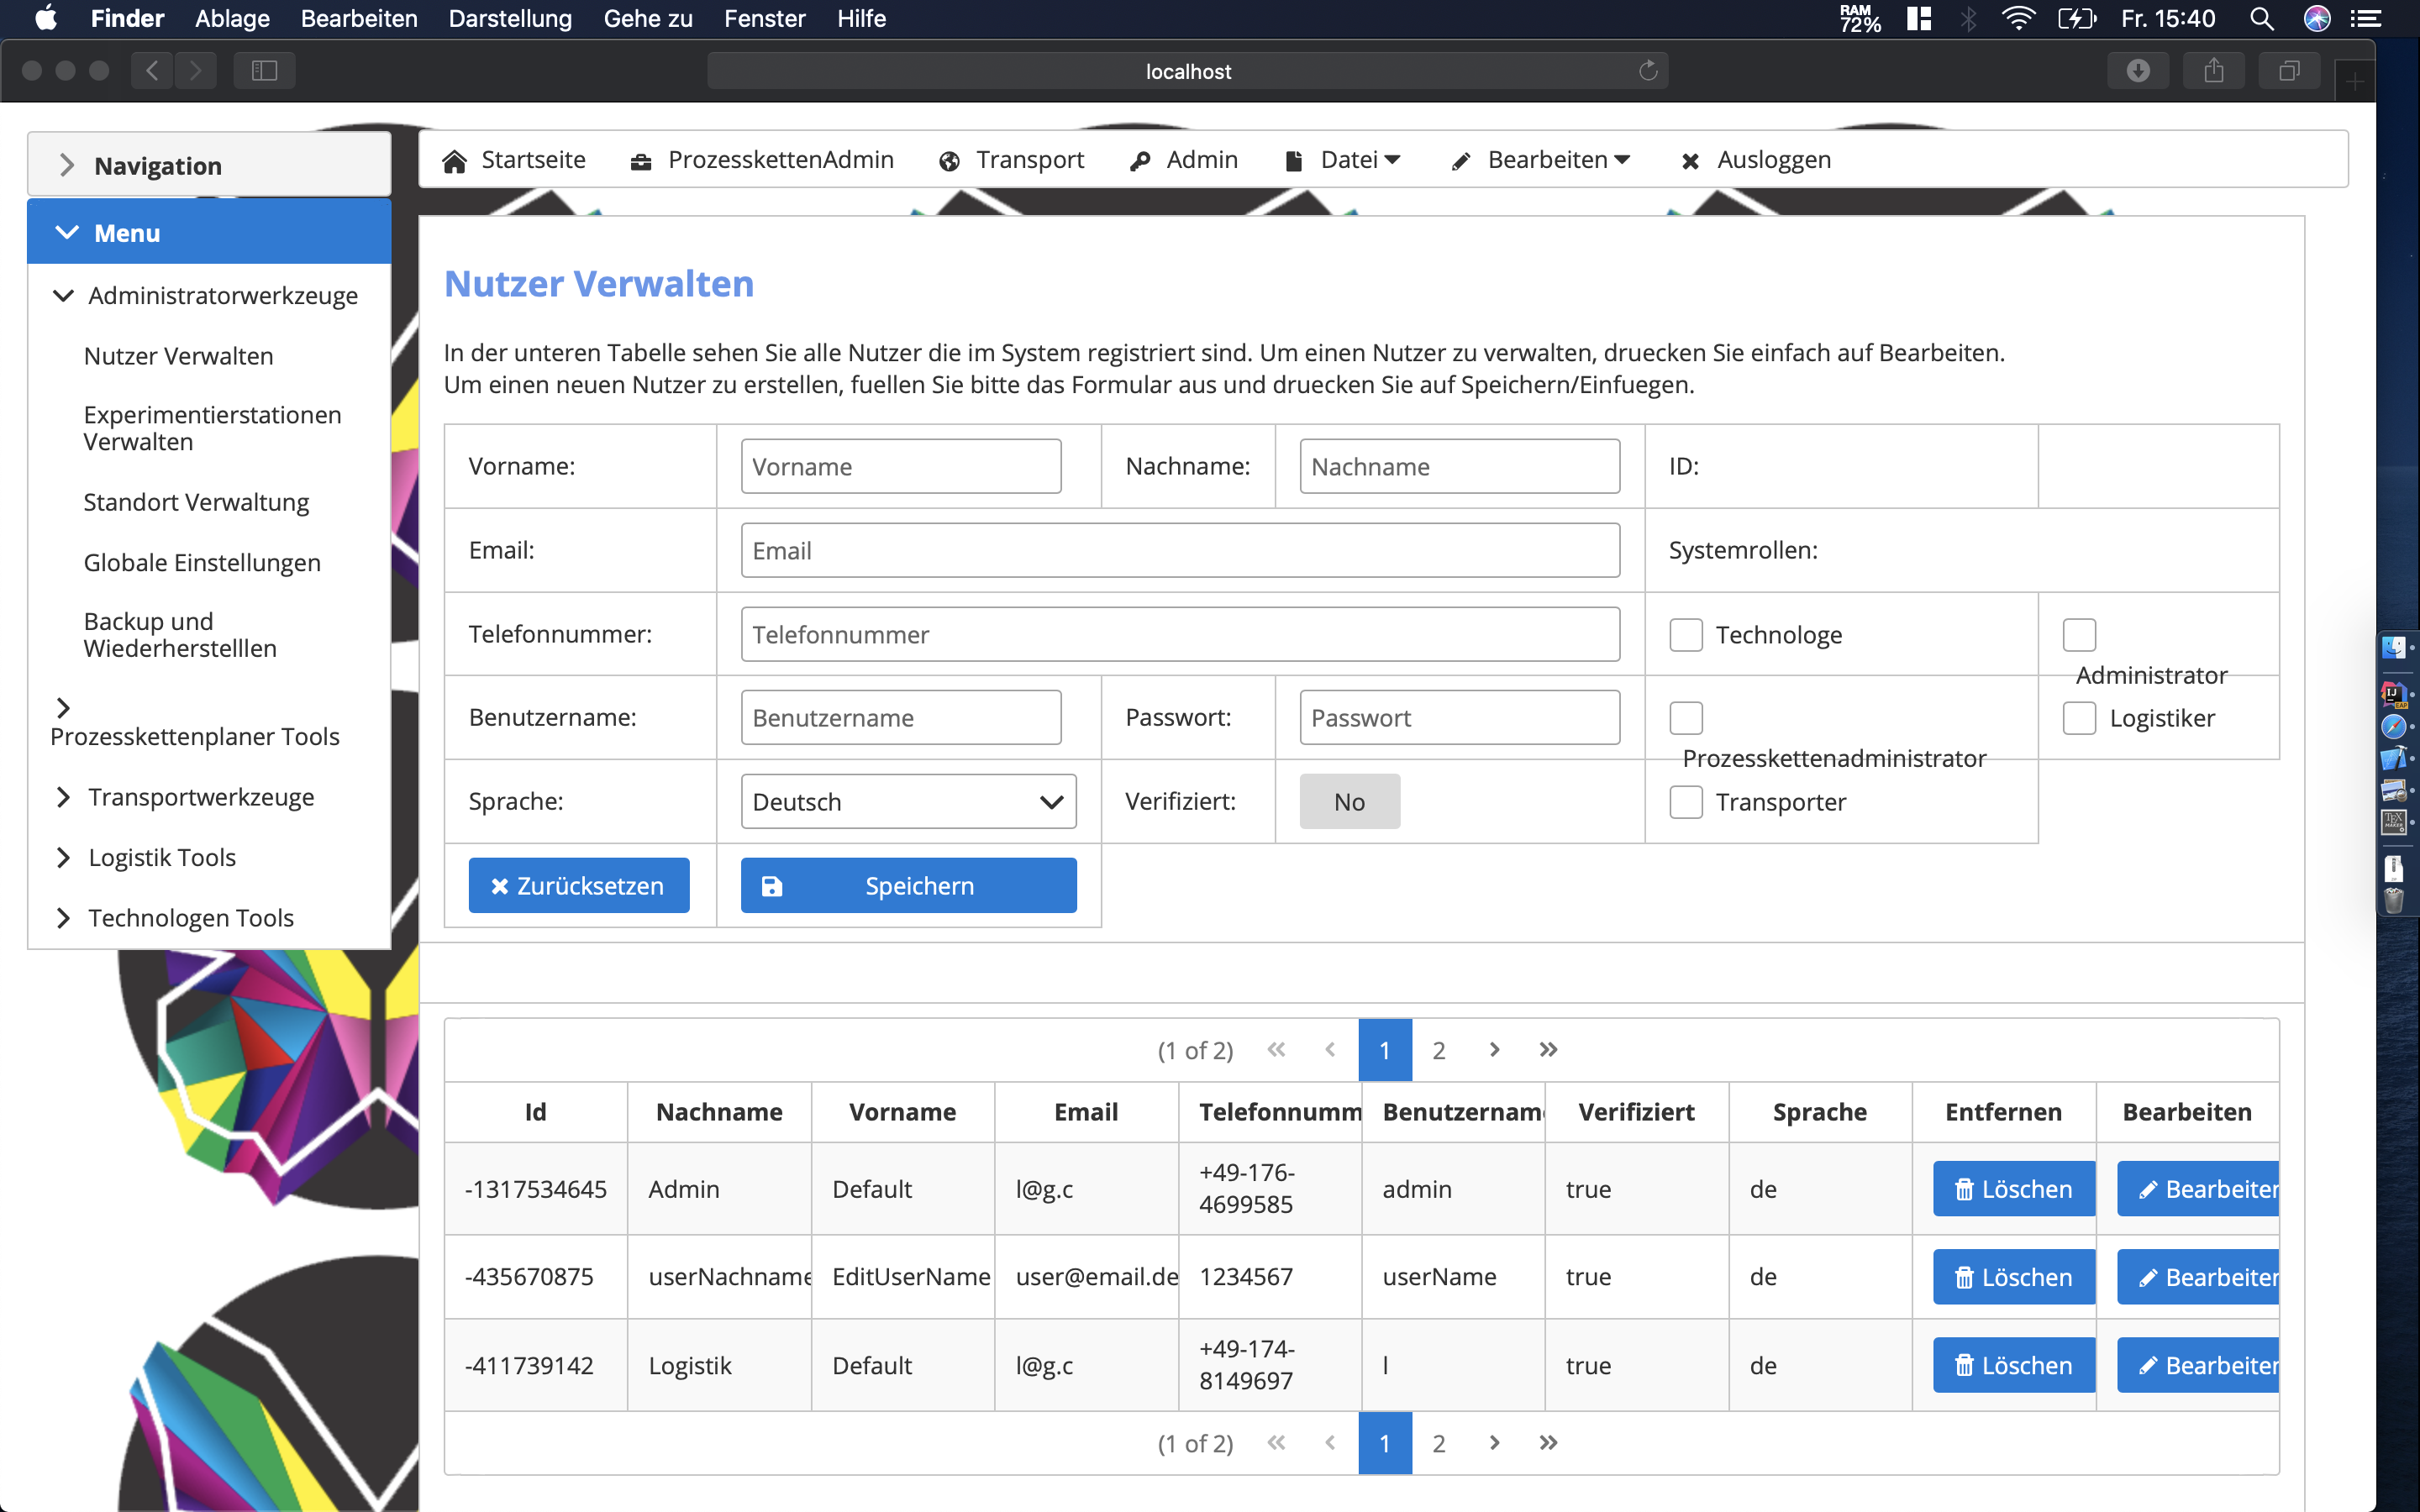
\includegraphics[width=1\textwidth]{Screenshots/5AddUsers.png}
\textit{Abbildung 3.2.4.6: Standort Formular}
} \\

%%

\subsection{Tests zum Prozesskettenadministrator}

\subsubsection{Anwendungsfall: Prozessschritte}
Zum Testen der Prozessschritt-Funktion verwenden wir die Administrator Sicht auf der entsprechenden Website. Hier gibt der Administrator die Daten in einem Formular ein, in dem die Instanz des Prozessschritts erstellt werden muss.\\

%%Formular
\hypertarget{sc3.3.1.1}{
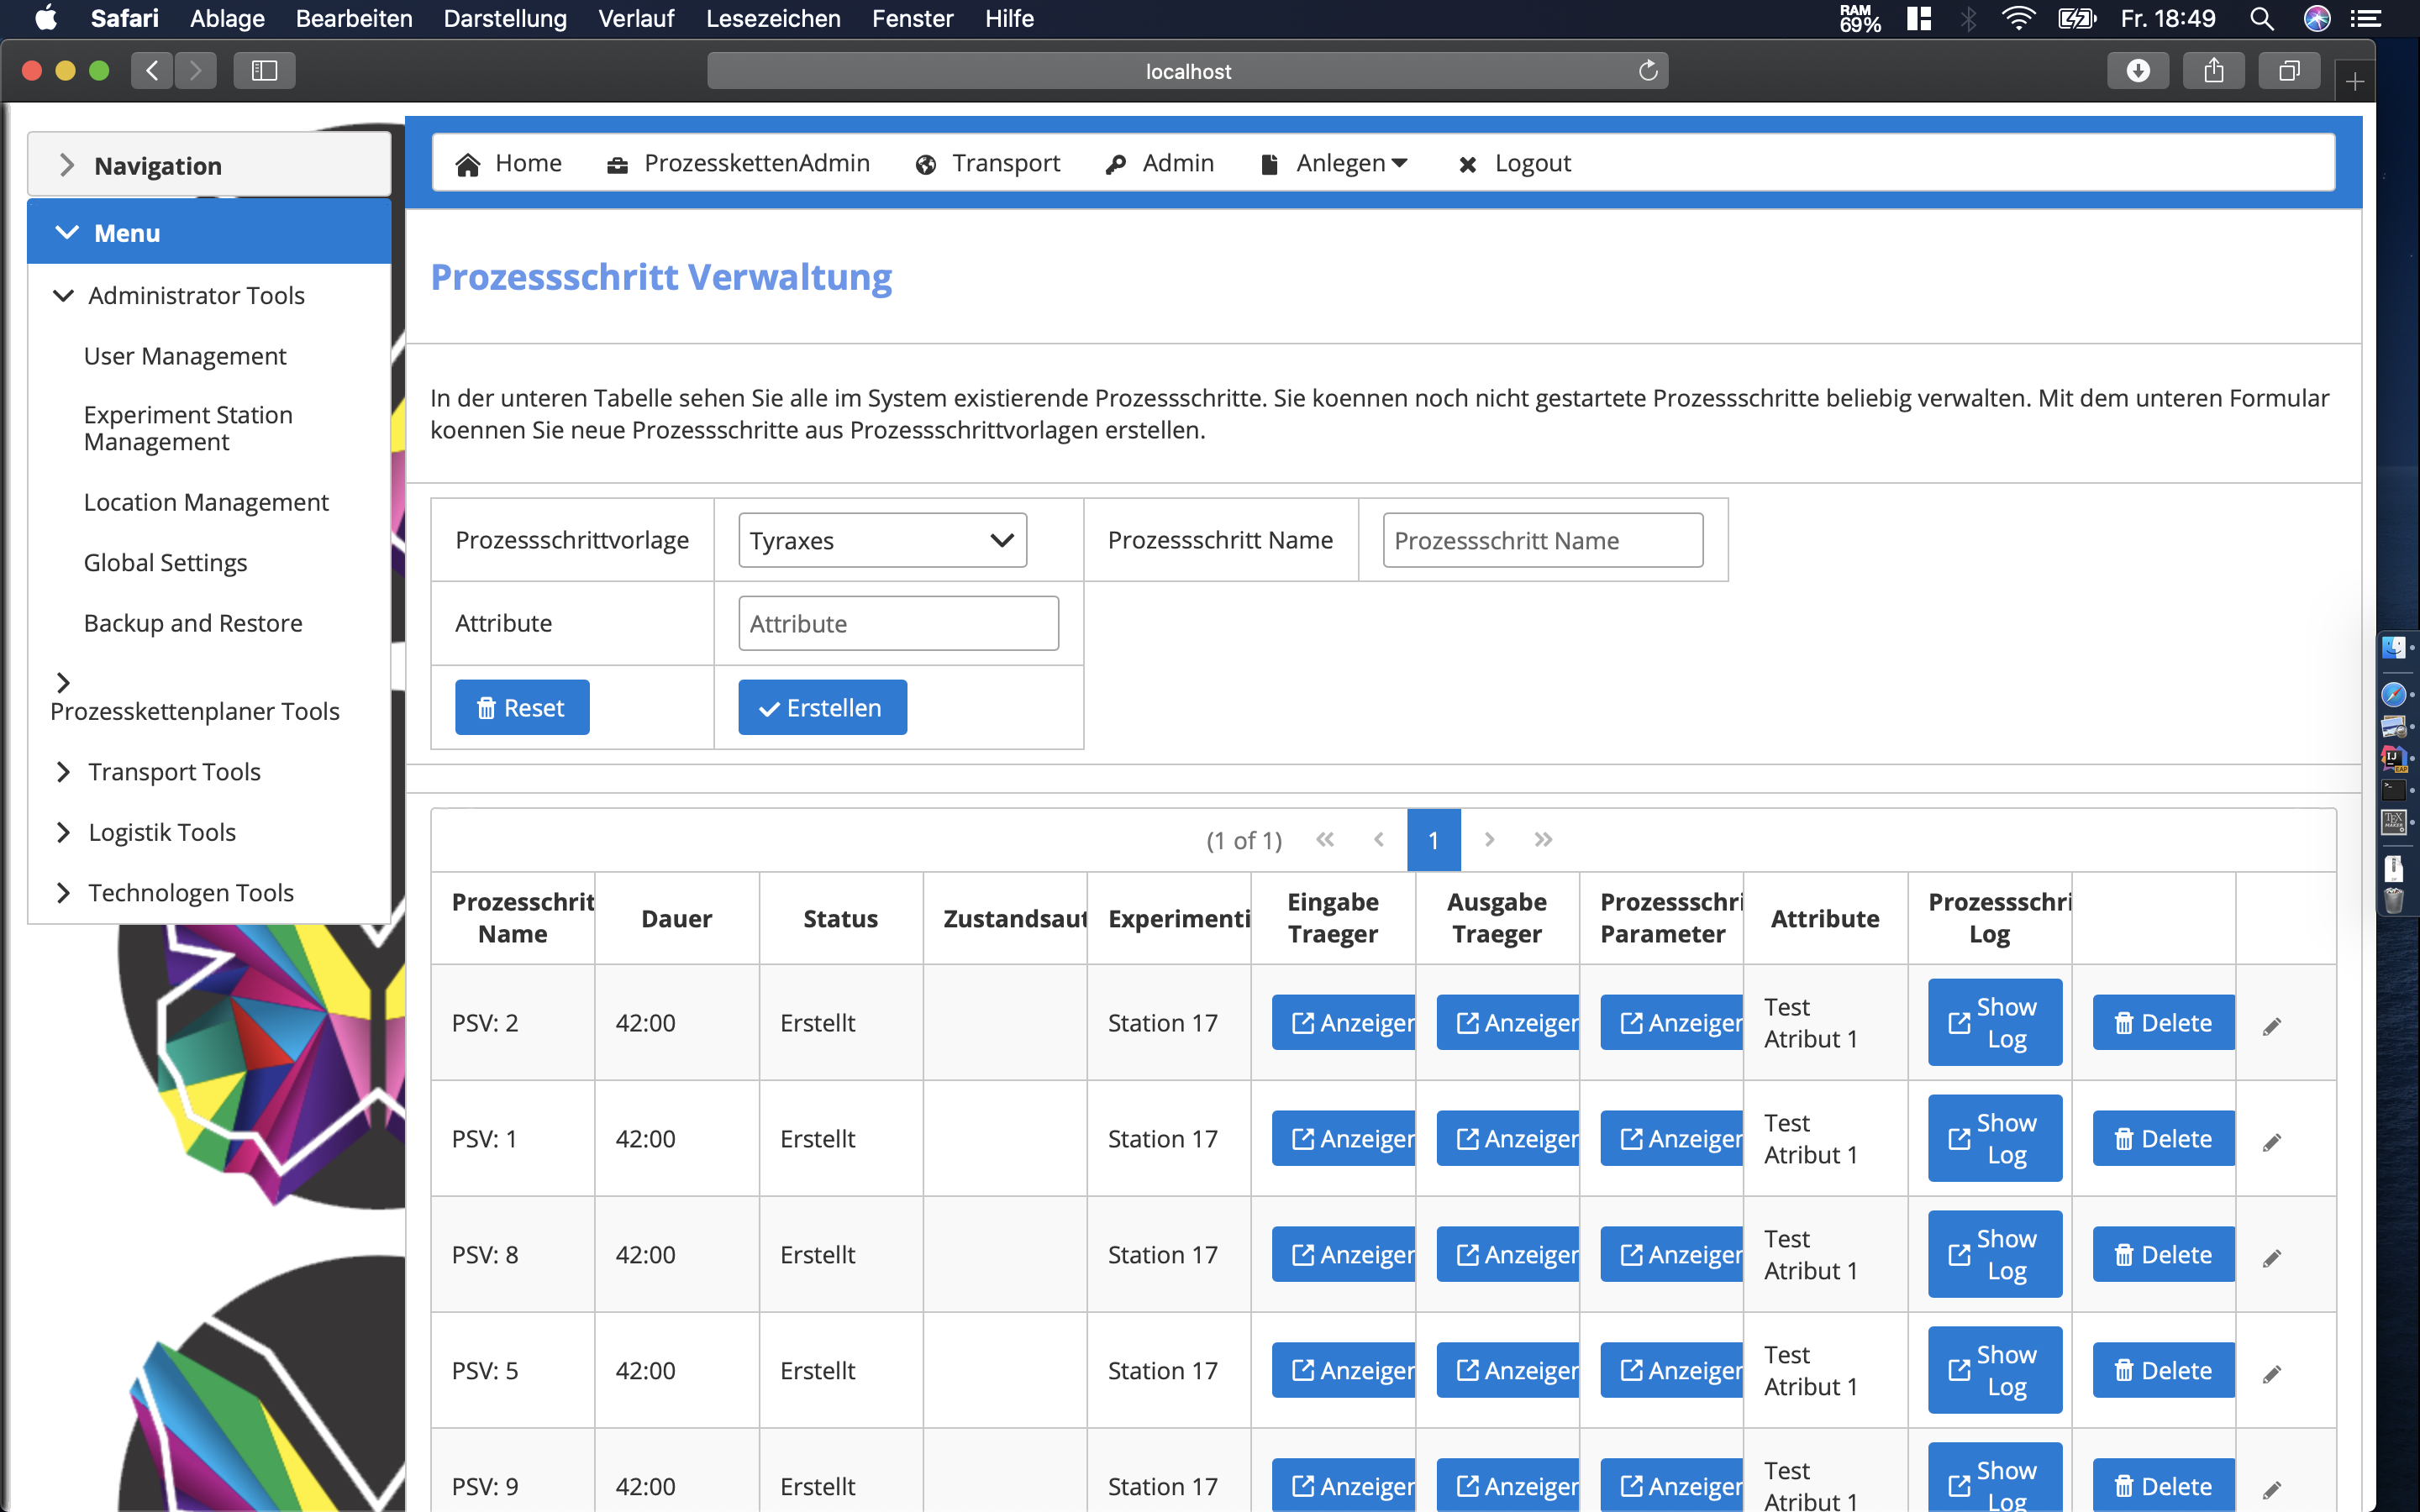
\includegraphics[width=1\textwidth]{Screenshots/33pspFormular.png}
\textit{Abbildung 3.3.1.1: Standort Formular}
} \\

Die folgenden Daten wurden für den Prozesstest zur Erstellung des Prozessschritts verwendet.\\

%%Data
\hypertarget{sc3.3.1.2}{
\includegraphics[width=1\textwidth]{Screenshots/33DataFakePsp.png}
\textit{Abbildung 3.3.1.2: Standort Formular}
} \\
Wenn die Knopf zum Erstellen gedrückt wird und der Erstellungsprozess erfolgreich war, sendet die Website eine Bestätigungsnachricht.\\

%%CreationMeldung
\hypertarget{sc3.3.1.3}{
\includegraphics[width=1\textwidth]{Screenshots/33creationMeldung.png}
\textit{Abbildung 3.3.1.3: Standort Formular}
} \\
Wenn der Prozessadministrator den Prozessschritt bearbeiten möchte, verwendet er die Funktion bearbeiten und füllt das Formular aus.
Wenn der Bearbeitungsprozess erfolgreich ist, erhält der Benutzer eine Bestätigungsnachricht über die Website.\\
%%Edit
\hypertarget{sc3.3.1.4}{
\includegraphics[width=1\textwidth]{Screenshots/33editView.png}
\textit{Abbildung 3.3.1.4: Standort Formular}
} \\
Im Bearbeitung View erhalten der Prozesskette Administrator eine Datenvisualisierung des Prozessschrittes durch die Nutzung der entsprechende Knöpfen. \\
%%LogsView
\hypertarget{sc3.3.1.5}{
\includegraphics[width=1\textwidth]{Screenshots/33log.png}
\textit{Abbildung 3.3.1.5: Standort Formular}
} \\
\hypertarget{sc3.3.1.6}{
\includegraphics[width=1\textwidth]{Screenshots/33log2.png}
\textit{Abbildung 3.3.1.6: Standort Formular}
} \\
Die Funktion der Schaltfläche Entfernen wurde ebenfalls getestet. Sie entfernt den Schritt-Prozess aus der Tabelle und sendet eine Nachricht an den Benutzer, wenn der Vorgang erfolgreich ist.\\
%%Remove
\hypertarget{sc3.3.1.7}{
\includegraphics[width=1\textwidth]{Screenshots/33removepsp.png}
\textit{Abbildung 3.3.1.7: Standort Formular}
} \\
\subsubsection{Anwendungsfall: Prozess Schritt Vorlage}

Die Funktionen der Erstellung, Bearbeitung, Visualisierung und Eliminierung von Prozess Schritt Vorlagen wurden getestet. Die Interaktion, die der Benutzer mit diesen Funktionen hat, erfolgt über das Formular auf der entsprechenden Seite.\\

\hypertarget{sc3.3.2.1}{
\includegraphics[width=1\textwidth]{Screenshots/332formularpzv.png}
\textit{Abbildung 3.3.2.1: Standort Formular}
} \\

Die folgenden Daten wurden für die Entwicklung des Testprozesses verwendet.\\

\hypertarget{sc3.3.2.2}{
\includegraphics[width=1\textwidth]{Screenshots/332DataPzv.png}
\textit{Abbildung 3.3.2.2: Standort Formular}
} \\

Sobald der Erstellungsprozess erfolgreich ist und die entsprechenden Daten eingegeben wurden, wird eine Bestätigungsnachricht von der Website zurückgegeben.\\

\hypertarget{sc3.3.2.3}{
\includegraphics[width=1\textwidth]{Screenshots/332MeldungCreation.png}
\textit{Abbildung 3.3.2.3: Standort Formular}
} \\
Wenn die Funktion Bearbeiten gedrückt wird, haben Sie die Möglichkeit, die Informationen des Prozess Schritt Parameters zu ändern.\\

\hypertarget{sc3.3.2.4}{
\includegraphics[width=1\textwidth]{Screenshots/332EditViewPsv.png}
\textit{Abbildung 3.3.2.4: Standort Formular}
} \\

In der Tabelle der Prozessschrittvorlagen finden Sie verschiedene Informationen zu den Prozessschrittvorlagen.\\

\hypertarget{sc3.3.2.5}{
\includegraphics[width=1\textwidth]{Screenshots/332log2psv.png}
\textit{Abbildung 3.3.2.5: Standort Formular}
} \\

\hypertarget{sc3.3.2.6}{
\includegraphics[width=1\textwidth]{Screenshots/332logpsv.png}
\textit{Abbildung 3.3.2.6: Standort Formular}
} \\

Wenn der Vorgang erfolgreich ist, wird nach der Ausgabe eine Bestätigungsnachricht von der Website abgerufen.\\

\hypertarget{sc3.3.2.7}{
\includegraphics[width=1\textwidth]{Screenshots/332updatepsv.png}\\
\textit{Abbildung 3.3.2.7: Standort Formular}
} \\

Die Funktion Entfernen wird getestet. Diese Funktion gibt eine Bestätigungsmeldung zurück, sobald der Entfernungsprozess erfolgreich war.\\

\hypertarget{sc3.3.2.8}{
\includegraphics[width=1\textwidth]{Screenshots/332removePsv.png}\\
\textit{Abbildung 3.3.2.8: Standort Formular}
} \\

Wenn eine der Daten nicht den erforderlichen Daten entspricht, gibt die Webseite eine Warnmeldung zurück, da der Vorgang nicht ausgeführt werden kann.\\

\hypertarget{sc3.3.2.9}{
\includegraphics[width=1\textwidth]{Screenshots/332regexpsv.png}\\
\textit{Abbildung 3.3.2.9: Standort Formular}
} \\
%%
\subsubsection{Anwendungsfall: Prozessschritt Vorlage}

Für die Funktionen der Prozess Schritt Vorlage wurde ein Testprozess durchgeführt. Die Optionen zum Erstellen, Bearbeiten und Entfernen von Instanzen wurden anhand des Formulars und der Tabelle getestet, mit denen der Benutzer interagiert.\\

\hypertarget{sc3.3.3.1}{
\includegraphics[width=1\textwidth]{Screenshots/333Formular.png}\\
\textit{Abbildung 3.3.3.1:  Prozessschritt Vorlage Formular}
} 
Wenn die Erstellung der Prozess Schritt Vorlage erfolgreich ist, wird eine Nachricht über die Website empfangen.\\

\hypertarget{sc3.3.3.2}{
\includegraphics[width=1\textwidth]{Screenshots/333Erzeugung.png}\\
\textit{Abbildung 3.3.3.2:  Prozessschritt Vorlage Meldung Data}
} 
Es wurde auch getestet, dass eine andere vom Benutzer gewählte Reihenfolge gewählt werden kann.\\

\hypertarget{sc3.3.3.3}{
\includegraphics[width=1\textwidth]{Screenshots/333Addmessage.png}
\textit{Abbildung 3.3.3.3:  Prozessschritt Vorlage Meldung Benachrichtigung }
} 

Für jede Prozessschritt-Vorlage können Informationen zu jeder Instanz angezeigt werden.\\

\hypertarget{sc3.3.3.4}{
\includegraphics[width=1\textwidth]{Screenshots/333Log.png}
\textit{Abbildung 3.3.3.4:  Prozessschritt Vorlage Log}
} 

Im Bearbeitungsmodus wurde auch getestet, dass die Anfangsdaten jeder Prozess Schrritt Vorlage geändert werden können.\\

\hypertarget{sc3.3.3.5}{
\includegraphics[width=1\textwidth]{Screenshots/333EditView.png}
\textit{Abbildung 3.3.3.5:  Prozessschritt Vorlage Edition Sicht}
} 

Sobald die Ausgabe erfolgreich war, wird eine Bestätigungsnachricht über die Website empfangen.\\

\hypertarget{sc3.3.3.6}{
\includegraphics[width=1\textwidth]{Screenshots/333EditErfolg.png}
\textit{Abbildung 3.3.2.6:  Prozessschritt Vorlage Bearbeitung Sicht}
} 

In ähnlicher Weise wird nach dem Entfernen einer Instanz eine Bestätigungsnachricht empfangen und die Instanz aus der Tabelle Prozess Schritt Vorlage entfernt.\\

\hypertarget{sc3.3.3.7}{
\includegraphics[width=1\textwidth]{Screenshots/333removemesage.png}
\textit{Abbildung 3.3.2.7: Prozessschritt Vorlage Entfernung Benachrichtigung}
} 

%%

\subsubsection{Anwendungsfall: Auftrag}

%%

\subsubsection{Anwendungsfall: Qualitativ und Quantitativ}
Die Erstellung- und Eliminierungsfunktion von Qualitative Eigenschaften wurde getestet. Der Benutzer muss mit einem Formular interagieren, um diese Funktionen ausführen zu können.\\
%%Formular
\hypertarget{sc3.3.3.7}{
\includegraphics[width=1\textwidth]{Screenshots/335Formular.png}
\textit{Abbildung 3.3.2.7: Prozessschritt Vorlage Entfernung Benachrichtigung}
}

%%EditView
\hypertarget{sc3.3.3.7}{
\includegraphics[width=1\textwidth]{Screenshots/336AddMeldung.png}
\textit{Abbildung 3.3.2.7: Prozessschritt Vorlage Entfernung Benachrichtigung}
} \\
wenn eine Instanz auf der entsprechenden Webseite bearbeitet wird. Wenn der Vorgang erfolgreich war, erhält der Benutzer eine Bestätigungsnachricht.\\
%%EditMeldung
\hypertarget{sc3.3.3.7}{
\includegraphics[width=1\textwidth]{Screenshots/336EditQuali.png}
\textit{Abbildung 3.3.2.7: Prozessschritt Vorlage Entfernung Benachrichtigung}
} \\
Sobald das Formular mit den entsprechenden Daten ausgefüllt und die Anforderung zur Erstellung der Instanz gesendet wurde, wird bei erfolgreichem Vorgang eine Bestätigungsnachricht von der Website empfangen.\\
In ähnlicher Weise wird für die Erstellung quantitativer Eigenschaften eine Bestätigungsnachricht empfangen, wenn der Instanzerstellungsprozess erfolgreich ist.\\
%%AddQuant
\hypertarget{sc3.3.3.7}{
\includegraphics[width=1\textwidth]{Screenshots/336AddQuantitativMeldung.png}
\textit{Abbildung 3.3.2.7: Prozessschritt Vorlage Entfernung Benachrichtigung}
} .\\
In der Ausgabe von Quantitative Einstellungen wurde es ebenfalls erfolgreich getestet.\\
%%EditView
\hypertarget{sc3.3.3.7}{
\includegraphics[width=1\textwidth]{Screenshots/336EditMeldungQuantDes.png}
\textit{Abbildung 3.3.2.7: Prozessschritt Vorlage Entfernung Benachrichtigung}
}  \\
In beiden Tabellen wird eine Bestätigungsmeldung angezeigt, sobald eine Instanz entfernt wurde und der Entfernungsprozess erfolgreich war.\\

%% remove
\hypertarget{sc3.3.3.7}{
\includegraphics[width=1\textwidth]{Screenshots/336RemoveMeldungqt.png}
\textit{Abbildung 3.3.2.7: Prozessschritt Vorlage Entfernung Benachrichtigung}
}  
 %% remove
\hypertarget{sc3.3.3.7}{
\includegraphics[width=1\textwidth]{Screenshots/336RemoveMledungql.png}
\textit{Abbildung 3.3.2.7: Prozessschritt Vorlage Entfernung Benachrichtigung}
}  
\subsubsection{Anwendungsfall: pk 6}

%%

\subsubsection{Anwendungsfall: pk 7}

%%

\subsubsection{Anwendungsfall: pk8 }

%%

\subsubsection{Anwendungsfall: pk9}

%%

\subsection{Tests zum Transporter}

\subsubsection{Anwendungsfall: Transporter möchte Transportieren}

Sobald man sich als Transporter anbeldet, gelangt man auf die \hyperlink{sc3.4.1.1}{Startseite} des Transporters. 

\hypertarget{sc3.4.1.1}{
\includegraphics[width=1\textwidth]{Screenshots/3411.png}
\textit{Abbildung 3.4.1.1: Startseite des Transporters}
} \\

Nun kann man im Hamburger Menü an der linken Seite auf \hyperlink{sc3.4.1.2}{Transportaufträge} gehen, um eine Übersicht über Transportaufträge zu bekommen.

\hypertarget{sc3.4.1.2}{
\includegraphics[width=1\textwidth]{Screenshots/3412.png}
\textit{Abbildung 3.4.1.2: Auftragsübersicht des Transporters}
} \\

Hier sieht man oben seine angenommenen Aufträge und in der unteren Tabelle verfügbare Aufträge. Anfangs hat der Benutzer keine Aufträge angenommen, weswegen die obere Tabelle leer ist. 

\paragraph{Verfügbare Aufträge annehmen:}

Man kann nun rechts den Annehmen Knopf drücken, um einen bestimmten Transportauftrag anzunehmen. Dieser wird aus der Liste der verfügbaren Aufträge für alle Benutzer gelöscht und wird in der Tabelle der angenommenen Aufträge angezeigt. Ich wähle den Transportauftrag mit der ID \textit{9} aus und drücke auf annehmen. 

\hypertarget{sc3.4.1.3}{
\includegraphics[width=1\textwidth]{Screenshots/3413.png}
\textit{Abbildung 3.4.1.3: Angenommener Auftrag}
} \\

Man sieht, dass der Auftrag mit der ID \textit{9} in der Tabelle für \hyperlink{sc3.4.1.3}{Angenommene Aufträge} ist. Der Zustand wurde auf Abgeholt gesetzt. Die restlichen Daten in der Tabelle ändern sich nicht. Wenn man nun in einen  \hyperlink{sc3.4.1.4}{anderen Transporter Benutzer} geht, sieht man, dass der Transportauftrag mit der ID \textit{9} nicht mehr auftaucht. Er ist dem User zugewiesen, der ihn annimmt. 

\hypertarget{sc3.4.1.4}{
\includegraphics[width=1\textwidth]{Screenshots/3414.png}
\textit{Abbildung 3.4.1.4: Ansicht eines Anderen Benutzers}
} \\

Der Test verlief erfolgreich. 

\paragraph{Angenommenen Auftrag abliefern:}

Der Transportauftrag mit der ID \textit{9} ist angenommen und auf dem Zustand abgeholt. Ich bin als Nutzer \textit{tr} eingeloggt. Wenn man nun den Button zum Abliefern in der Tabelle der angenommenen Aufträge drückt, verschwindet der Auftrag aus der Übersicht der angenommenen Aufträge. 

\hypertarget{sc3.4.1.5}{
\includegraphics[width=1\textwidth]{Screenshots/3415.png}
\textit{Abbildung 3.4.1.5: Übersicht über alle erledigten Aufträge}
} \\

In der \hyperlink{sc3.4.1.5}{Übersicht der erledigten Aufträge}, welche auch im Log gespeichert wird und dort vom Admin eingesehen werden kann, sieht man nun, dass Transportauftrag 9 den Zustand \textit{Abgeliefert} hat. Man kann außerdem sehen, wann welcher Zustandswechsel durchgeführt wurde und von wem der Transportauftrag durchgeführt wurde. Der Nutzer und die Zeiten sind ebenfalls richtig. 

Der Test verlief also erfolgreich. 

{
\color{red} Es muss getestet werden, ob die richtigen Träger angezeigt werden.
}
 

%%

\subsubsection{Anwendungsfall: Probenverlust melden}

Hierfür erstelle ich zunächst im Logister jeweils 100 Proben mit den IDs von \textit{A01.0101} bis \textit{A01.0105}. Diese Funktion wird in dem jeweiligen Abschnitt des Testprotokolls separat getestet. Hier sieht man den \hyperlink{sc3.4.2.1}{Ausgangszustand}. \\

\hypertarget{sc3.4.2.1}{
\includegraphics[width=1\textwidth]{Screenshots/3421.png}
\textit{Abbildung 3.4.2.1: Ausgangszustand nach dem Erstellen der Proben}
} \\

Nun melde ich von Probe \textit{A01.0101} eine Probe als Verloren, von \textit{A01.0102} 50 Proben als verloren, von \textit{A01.0103} zweimal 50, sodass alle 100 verloren sind und die Probe auf Verloren gesetzt wird, von \textit{A01.0104} werden 100 Proben als verloren gesetzt, und bei Probe \textit{A01.0105} werden erst 100 Proben auf verloren gesetzt, dann 100 neue erstellt, und diese 100 wieder als Verloren gemeldet. Also sind bei \textit{A01.0105} 200 Proben verloren. 

\hypertarget{sc3.4.2.2}{
\includegraphics[width=1\textwidth]{Screenshots/3422.png}
\textit{Abbildung 3.4.2.2: Probenverlust Melden Ansicht}
} \\

Im \hyperlink{sc3.4.2.3}{Endzustand} sieht man, dass alles so aufgetreten ist, wie gewollt. Der Test gilt als bestanden. Verlorene Proben werden rot markiert.

\hypertarget{sc3.4.2.3}{
\includegraphics[width=1\textwidth]{Screenshots/3423.png}
\textit{Abbildung 3.4.2.3: Endzustand der Proben}
} \\

\paragraph{Mehr Proben als Verloren melden als existieren:}

Wenn ich 100 Proben der ID \textit{A01.0106} erstelle und versuche zweimal 50 und anschließend eine Probe als Verloren zu melden, dann tritt ein Fehler auf und die Probe wird die Anzahl geht nicht ins negative. 

\hypertarget{sc3.4.2.4}{
\includegraphics[width=1\textwidth]{Screenshots/3424.png}
\textit{Abbildung 3.4.2.4: Fehlermeldung, wenn man zu mehr Proben eingibt, als existieren}
} \\

\hypertarget{sc3.4.2.5}{
\includegraphics[width=1\textwidth]{Screenshots/3425.png}
\textit{Abbildung 3.4.2.5: Endzustand der Proben}
} \\

%%

\subsection{Tests zum Logistiker}

\subsubsection{Anwendungsfall: Träger Management}

\paragraph{Logistiker legt einen Träger im Lager an:}

Der Logistiker legt einen Träger mit der Trägerart Glass im Lager an. Hierzu legt er die Bedingungen in den \hyperlink{sc3.5.1.1}{Feldern} fest und drückt auf erstellen. \\

\hypertarget{sc3.5.1.1}{
\includegraphics[width=1\textwidth]{Screenshots/3511.png}
\textit{Abbildung 3.5.1.1: Trägerübersicht}
} \\

In der \hyperlink{sc3.5.1.2}{Tabelle} wird der erstellte Auftrag angezeigt. \\

\hypertarget{sc3.5.1.2}{
\includegraphics[width=1\textwidth]{Screenshots/3512.png}
\textit{Abbildung 3.5.1.2: Trägerübersicht mit erstelltem Träger}
} \\

\paragraph{Bestehendem Träger Proben zuweisen}

Hierfür muss vorher ein Träger und Proben erstellt worden sein. Man geht auf den Bearbeitungsstift in der Tabelle und klappt dann das Auswahlmenü für ausgewählte Proben aus. Hier klickt man die Proben an, hier \textit{A01.0101} und diese wird dem Träger Hinzugefügt. 

 \hypertarget{sc3.5.1.3}{
\includegraphics[width=1\textwidth]{Screenshots/3513.png}
\textit{Abbildung 3.5.1.3: Träger bearbeiten}
} \\

Anschließend drückt man den Haken zum speichern. 
Jetzt bekommt man eine Meldung, dass der Träger erstellt wurde und er taucht in der \hyperlink{sc3.5.1.4}{Tabelle} auf. 

 \hypertarget{sc3.5.1.4}{
\includegraphics[width=1\textwidth]{Screenshots/3514.png}
\textit{Abbildung 3.5.1.4: Träger wurde bearbeitet}
} \\

\paragraph{Existierenden Träger löschen:}

Um einen existierenden Träger zu löschen, drückt man in der Tabelle einfach auf den \hyperlink{sc3.5.1.5}{Löschen Button}. 

 \hypertarget{sc3.5.1.5}{
\includegraphics[width=1\textwidth]{Screenshots/3515.png}
\textit{Abbildung 3.5.1.5: Träger Löschen Button}
} \\

Nachdem der Button gedrückt ist, verschwindet der Träger und wurde gelöscht. Auch nach einem Neu laden der Seite bleibt er in der \hyperlink{sc3.5.1.6}{Tabelle} verschwunden.

 \hypertarget{sc3.5.1.6}{
\includegraphics[width=1\textwidth]{Screenshots/3516.png}
\textit{Abbildung 3.5.1.6: Träger wurde bearbeitet}
} \\

Der Test ist bestanden. 

%%

\subsubsection{Anwendungsfall: Aufträge des Logistikers}

Vorbedingungen sind, dass ein Prozessschritt und ein Auftrag mit dem Prozessschritts im Prozesskettenadmin erstellt wurden. Anschließend wird der Auftrag vom Prozesskettenadmin freigegeben. Nun wird er in der \hyperlink{sc3.5.2.1}{Auftragsansicht des Logistikers} angezeigt. 

 \hypertarget{sc3.5.2.1}{
\includegraphics[width=1\textwidth]{Screenshots/3521.png}
\textit{Abbildung 3.5.2.1: Auftragsansicht des Logistikers}
} \\

Nun muss der Logistiker den Auftrag bearbeiten und ihm einen \hyperlink{sc3.5.2.2}{Träger zuweisen}. \\

 \hypertarget{sc3.5.2.2}{
\includegraphics[width=1\textwidth]{Screenshots/3522.png}
\textit{Abbildung 3.5.2.2: Träger einem Auftrag zuweisen}
} \\

Wenn man auf den Haken zum speichern drückt, wird der Träger dem Auftrag hinzugefügt. \\

 \hypertarget{sc3.5.2.3}{
\includegraphics[width=1\textwidth]{Screenshots/3523.png}
\textit{Abbildung 3.5.2.3: Träger einem Auftrag zugewiesen}
} \\

Anschließend muss der Logistiker den Auftrag annehmen. Der Auftrag wird auf Gestartet gesetzt und verschwindet dann aus der Sicht des Logistikers. \\ 

 \hypertarget{sc3.5.2.4}{
\includegraphics[width=1\textwidth]{Screenshots/3524.png}
\textit{Abbildung 3.5.2.4: Auftrag gestartet}
} \\

Der Transporter bekommt nun einen Transportauftrag vom Lager zum ersten Prozessschritt. \\

 \hypertarget{sc3.5.2.5}{
\includegraphics[width=1\textwidth]{Screenshots/3525.png}
\textit{Abbildung 3.5.2.5: Transportansicht mit dem Auftrag von dem Logistiker}
} \\

Der Test ist bestanden.

%%

\subsubsection{Anwendungsfall: Proben erstellen}

Wie man sieht, existiert bereits eine \hyperlink{sc3.5.3.1}{Probe} mit der ID A01.0101. 

 \hypertarget{sc3.5.3.1}{
\includegraphics[width=1\textwidth]{Screenshots/3531.png}
\textit{Abbildung 3.5.3.1: Probenübersicht Vorher}
} \\

Nun gehe ich auf die Proben Einfügen Seite und erstelle 5 Proben.   \\

 \hypertarget{sc3.5.3.2}{
\includegraphics[width=1\textwidth]{Screenshots/3532.png}
\textit{Abbildung 3.5.3.2: Proben erstellen}
} \\

Ich erstelle Jeweils 100 Proben mit den IDs A02.0101 bis A02.0104.  Anschließend erstelle ich mit der ID A02.0101 noch einmal 100 Proben, sodass am ende von A02.0101 200 Proben existieren.\\

 \hypertarget{sc3.5.3.3}{
\includegraphics[width=1\textwidth]{Screenshots/3533.png}
\textit{Abbildung 3.5.3.3: Probenübersicht Nachher}
} \\

Der Test ist bestanden.

%%

\subsubsection{Anwendungsfall: Probenstandort}

Um den Probenstandort zu verändern, muss eine Probe in einem Träger enthalten sein und einen Transportauftrag durchlaufen. 

 \hypertarget{sc3.5.4.1}{
\includegraphics[width=1\textwidth]{Screenshots/3541.png}
\textit{Abbildung 3.5.4.1: Probenstandortübersicht Vorher. Alle Proben befinden sich im Lager}
} \\

Nun lasse ich den Auftrag mit dem Träger mit der Probe A01.0103 vom Lager zu Station 0 transportieren. 

 \hypertarget{sc3.5.4.2}{
\includegraphics[width=1\textwidth]{Screenshots/3542.png}
\textit{Abbildung 3.5.4.2: Probenstandortübersicht Nachher}
} \\

Der Test ist erfolgreich.


%%

\subsubsection{Anwendungsfall: log 5}

%%

\subsubsection{Anwendungsfall: log 6}

%%

\subsubsection{Anwendungsfall: log 7}

%%

\subsection{Tests zum Technologen}

\subsubsection{Anwendungsfall: Beispiel 5}

%%

\subsubsection{Anwendungsfall: Beispiel 5}

%%%%%%%%%%%%

\section{Automatisierte Funktionstests}

\subsection{Einführung}

Projektklassen wurden unabhängig getestet. Das für die Tests verwendete Framework war Junit, Version 5. Das Mockito Framework für die automatischen Tests wurde ebenfalls verwendetet. Objectos.Mock wurden für die zu testenden Klassen geschrieben und in der geschätzten Zeit vor der Lieferung wurden so viele Tests wie möglich durchgeführt.

Für die meisten Klassen wurde ein unabhängiger Test durchgeführt, bei dem die Methoden separat getestet wurden. In der gewünschten  Lieferzeit wurden so viele Tests wie möglich durchgeführt. Zusätzlich zu einer breiteren Testabdeckung wurden Selenium Tests und manuelle Tests durchgeführt, um die Abdeckung der automatischen Tests zu erweitern und die Mindestanforderungen der zu kontrollieren Software.


\subsubsection{Anwendungsfall: Beispiel 1}

%%

\subsubsection{Anwendungsfall: Beispiel 2}

%%

\subsubsection{Anwendungsfall: Beispiel 3}

%%

\subsubsection{Anwendungsfall: Beispiel 4}

%%

\subsubsection{Anwendungsfall: Beispiel 5}

%%%%%%%%%%%%%%%%%%%%%%%%%%%%%%%%%%%%%%%%%%%%%%%%%%%%%%%%%%%%%%%%%%%%%%%%

\end{document}














